\documentclass[10pt,twoside,b5paper,final]{book}

\usepackage[utf8]{inputenc}

\usepackage[b5paper]{geometry}
\geometry{top=1in,bottom=0.875in,outer=0.75in,inner=1in}

\usepackage{afterpage} % The \afterpage command causes LaTeX to
                       % expand its argument after the current page
                       % is filled and output. Although you can
                       % specify any command in the \afterpage
                       % argument, using the \clearpage command is a
                       % particularly useful way to force the
                       % printing of any floating objects (graphics
                       % and long tables) that haven't yet been
                       % anchored to a position. LaTeX fills the page
                       % on which the \afterpage command occurs and
                       % then prints any unanchored floating objects
                       % before continuing with the text. Use the
                       % \afterpage command in an encapsulated TeX
                       % field. The package has no options.

\usepackage{amsmath}   % If you are going beyond the most basic level
                       % of displayed equations, you will benefit from
                       % using the amsmath package that plugs into
                       % LaTeX. This package has lots of useful
                       % features for multi-line equations, compound
                       % symbols, even commutative diagrams! Allows
                       % use \text in equations	

\usepackage{textcomp} % This package allows you to use the
                      % comprehensive symbol list with over 3000 symbols
                      % You need this to generate the promille sign 
                      % (\textperthousand)

\usepackage{booktabs}  % booktabs is to enable the easy production of
                       % tables such as should appear in published
                       % scientific books and journals. What
                       % distinguishes these from plain LaTeX tables
                       % is the default use of additional space above
                       % and below rules, and rules of
                       % varying`thickness'.booktabs is to enable the
                       % easy production of tables such as should
                       % appear in published scientific books and
                       % journals. What distinguishes these from plain
                       % LaTeX tables is the default use of additional
                       % space above and below rules, and rules of
                       % varying `thickness'.To have better tables
\usepackage{multirow}

\usepackage{longtable} % To create tables that span multiple pages

\usepackage{enumerate} % The enumerate environment produces a
                       % numbered list. Enumerations can be nested
                       % within one another, up to four levels
                       % deep. They can also be nested within other
                       % paragraph-making environments.

\usepackage{rotating}  % The rotating package implements three
                       % environments within which in-line figures,
                       % tables, and captions can be rotated by an
                       % arbitrary number of degrees. Two additional
                       % environments allow rotation of floating
                       % objects, which are typeset alone on separate
                       % pages.

\usepackage[binary,thickspace,thickqspace]{SIunits}   % Typeset physical units following the rules
                       % of the International System of Units (SI).

\usepackage{ragged2e}

\usepackage{float}

\usepackage{textgreek}

\usepackage{tgbonum}
\usepackage[T1]{fontenc}

\usepackage{graphicx}  % The graphicx package implements LaTeX
                       % support for including graphics files,
                       % rotating parts of a page, and scaling parts
                       % of a page. The package depends on having a
                       % DVI driver that can produce these effects.
                       
\usepackage{hyperref}  % For crossreferences in text 

% paragraph skip                       
% \setlength{\parskip}{0.2em}
\renewcommand{\baselinestretch}{1.33}

% package of reference
\usepackage[backend=biber,style=nature,natbib=true]{biblatex}
\addbibresource{library/bibliography.bib}
\renewcommand*{\bibfont}{\fontfamily{phv}\selectfont\small}

% ------------------------------- thumb index ------------------------
%%% Thumb indices consist of white text on a rectangular colored background. The
%%% font-size is 75% of the size of thumb height.
\newlength\thumbheight
\setlength\thumbheight{24pt}
\newlength\thumbedge
\setlength\thumbedge{2pt}
\newlength\thumbhspace
\setlength\thumbhspace{36pt}
\newlength\thumbvspace
\setlength\thumbvspace{3\thumbheight}

\newlength\thumbwidth
\setlength\thumbwidth{36pt}
\newlength\thumbspacing
\setlength\thumbspacing{2\thumbheight}

%% We need the TikZ library calc to calculate the coordinates of the thumb
%% indices.
\usepackage{tikz}
\usetikzlibrary{calc}
\usepackage{xcolor}

\definecolor{anthracite}{cmyk}{0,0,0,0.8}
\colorlet{thumb}{anthracite}

%% The lthumb command prints the current chapter number in a thumb index on the
%% left (even) page.
\newcommand*\lthumb{%
    % \ifthumb%
        \begin{tikzpicture}[remember picture,overlay]
            \coordinate (top margin) at (0pt,1.5in+\topmargin+\headheight+\headsep);
            \coordinate (left margin) at (1.1in+\evensidemargin,0pt);
            %% Calculate the corners of the thumb index based on the current
            %% chapter number.
            \coordinate (top left) at ($(current page.north west)-(top margin)-(0pt,\value{chapter}\thumbvspace-\thumbvspace)$);
            \coordinate (bottom right) at ($(top left)+(left margin)-(\thumbhspace,\thumbheight)$);
            %% Shift the left edge to prevent the rounded corner from showing.
            \coordinate (top left) at ($(top left)-(\thumbedge,0pt)$);
            %% Draw the thumb index.
            \fill[fill=thumb,rounded corners=\thumbedge](top left) rectangle (bottom right);
            %% Print the chapter number at the center right in the thumb index.
            \coordinate (center right) at ($(bottom right)+(0pt,0.5\thumbheight)$);
            \node at (center right)[anchor=east,inner sep=2\thumbedge]{
                \fontfamily{phv}\color{white}
                \fontsize{0.7\thumbheight}{0.7\thumbheight}\selectfont
                \thechapter
            };
        \end{tikzpicture}%
    % \fi%
}

%% rthumb draws a thumb index on the right (odd) page.
\newcommand*\rthumb{%
    \begin{tikzpicture}[remember picture,overlay]
        \coordinate (top margin) at (0pt,1in+\topmargin+\headheight+\headsep);
        \coordinate (right margin) at (1.1in+\evensidemargin,0pt);
        %% Calculate the corners of the thumb index based on the current
        %% chapter number.
        \coordinate (top right) at ($(current page.north east)-(top margin)-(0pt,\value{chapter}\thumbvspace-\thumbvspace)$);
        \coordinate (bottom left) at ($(top right)-(right margin)-(-\thumbhspace,\thumbheight)$);
        %% Shift the left right to prevent the rounded corner from showing.
        \coordinate (top right) at ($(top right)+(\thumbedge,0pt)$);
        %% Draw the thumb index.
        \fill[fill=thumb,rounded corners=\thumbedge](top right) rectangle (bottom left);
        %% Print the chapter number at the center right in the thumb index.
        \coordinate (center left) at ($(bottom left)+(0pt,0.5\thumbheight)$);
        \node at (center left)[anchor=west,inner sep=2\thumbedge]{
            \fontfamily{phv}\color{white}
            \fontsize{0.7\thumbheight}{0.7\thumbheight}\selectfont
            \thechapter
        };
    \end{tikzpicture}%
}
% ---------------------------------------------------------------------

% define Page style
\usepackage{fancyhdr}
% Defining the new page style
\pagestyle{fancy}
\fancypagestyle{MyStyle}{%
    \fancyhead{} %Clean headers
    \fancyhead[RO]{\rthumb\fontfamily{phv}\selectfont\small\leftmark}
    \fancyhead[LE]{\lthumb\fontfamily{phv}\selectfont\small\chaptername\ \thechapter}
    \fancyfoot{} % clear all footer fields
    \fancyfoot[LE,RO]{\fontfamily{phv}\selectfont\thepage}
    \renewcommand{\chaptermark}[1]{\markboth{##1}{}}
    \renewcommand{\headrulewidth}{0pt}% disable the underline of the header part
}

% Redefine the plain page style
\fancypagestyle{backmatter}{%
    \fancyhf{}%
    \fancyfoot{} % clear all footer fields
    \fancyfoot[LE,RO]{\fontfamily{phv}\selectfont\thepage}
    \renewcommand{\headrulewidth}{0pt}% Line at the header invisible
    \renewcommand{\footrulewidth}{0pt}% Line at the footer visible
}

\fancypagestyle{plain}{%
  \fancyhf{}%
  \fancyfoot[C]{\fontfamily{phv}\selectfont\thepage}%
  \renewcommand{\headrulewidth}{0pt}% Line at the header invisible
  \renewcommand{\footrulewidth}{0pt}% Line at the footer visible
}

% define the font and color of chapter/setion title
\usepackage{lmodern}
\usepackage{titlesec}
\titleformat{\chapter}[display]
  {\fontfamily{phv}\selectfont\fontsize{96}{1}\selectfont\RaggedLeft}
  {\thechapter}{40pt}{\LARGE\bfseries}
\titleformat{\section}
  {\normalfont\fontfamily{phv}\selectfont\Large\bfseries}
  {\thesection}{1em}{}
\titleformat{\subsection}
  {\normalfont\fontfamily{phv}\selectfont\large\bfseries}
  {\thesection}{1em}{}
\titleformat{\subsubsection}
  {\normalfont\fontfamily{phv}\selectfont\normalsize\itshape}
  {\thesection}{1em}{}
\titleformat{\paragraph}
  {\normalfont\fontfamily{phv}\selectfont\normalsize\itshape}
  {\thesection}{1em}{}
  
% define caption font
\usepackage{caption}
\DeclareCaptionFont{captionfont}{\fontfamily{phv}\selectfont\small}
\captionsetup{font=captionfont,labelfont=bf}

% table of content
\usepackage{tocloft}
% \renewcommand\cftchapafterpnum{\vskip6pt}
% \renewcommand\cftsecafterpnum{\vskip6pt}
% \renewcommand\cftsubsecafterpnum{\vskip6pt}
\renewcommand{\cfttoctitlefont}{\fontfamily{phv}\selectfont\LARGE\bfseries}
\renewcommand{\cftchapfont}{\fontfamily{phv}\selectfont\normalsize}
\renewcommand{\cftsecfont}{\fontfamily{phv}\selectfont\normalsize}
\renewcommand{\cftsubsecfont}{\fontfamily{phv}\selectfont\normalsize}
\renewcommand{\cftchappagefont}{\fontfamily{phv}\selectfont\normalsize}
\renewcommand{\cftsecpagefont}{\fontfamily{phv}\selectfont\normalsize}
\renewcommand{\cftsubsecpagefont}{\fontfamily{phv}\selectfont\normalsize}

% define statistics 
\newcommand{\pval}{\textit{p}\ }
\newcommand{\tval}{\textit{t}\ }
\newcommand{\rval}{\textit{r}\ }
\newcommand{\tvaldf}{\textit{t}}
\newcommand{\rvaldf}{\textit{r}}

% package of Chinese
\usepackage{CJKutf8}

% long caption
\makeatletter
\newenvironment{figurelongcaption}
{\def\@captype{figure}}
{}
\makeatletter

% If you are sending a PhD thesis to a professional printer, the
% statements below may be handy - uncomment them in this case

% \oddsidemargin=-3.4mm    % Margin to use for binding of the text 2.2 cm
% \evensidemargin=-5.4 mm  % Margin for cutting of for professional printing = 2.0 cm
% \textwidth=158mm         % Width of the text = 12.8 * 19.5 cm

% The \raggedbottom declaration makes all pages the height of the text
% on that page. No extra vertical space is added.
\raggedbottom

% Specify the title and subtitle...
\def\maintitle{Multiscale connectomics and disconnectivity in schizophrenia}
%\def\subtitle{No beer, no coffee, just hard work!!!}
% Specify the authors and date
\def\authors{Yongbin Wei}
\def\locationdate{Amsterdam, 22-11-2019}

% ----------------------------------------------------------------------

\begin{document}

\fontfamily{phv}\selectfont	

\frontmatter
% No page number on title pages
\pagestyle{empty}

%-- french title page (r) ------------------------------------------------
\begin{center}
  \vspace*{3cm}
  {\LARGE\bfseries\maintitle\par}
%  {\Large\bfseries\subtitle\par}
  \vspace{6em}%
  {\Large\authors\par}
  \vspace{3mm}%
  \begin{CJK*}{UTF8}{gbsn}
  \textbf{魏\ 永斌}
  \clearpage\end{CJK*} 
% uncomment below if you want a date on the front page
% {\locationdate\par}
\end{center}

\newpage
\vspace*{\fill}
\begin{flushleft}
\vspace{0.1cm}
\textbf{Copyright} © Yongbin Wei, Amsterdam 2019. \\
\vspace{0.1cm}
All rights reserved.   No part of this publication may be reproduced, stored in a retrieval system or transmitted in any form or by any means, electronic,mechanical,  photocopying,  recording  or  otherwise,  without  prior  written permission of the author.\\
\vspace{0.1cm}
\textbf{Cover page}: XXX XXX \\ %... image caption for cover page image here ...
\vspace{0.1cm}
\textbf{ISBN}: XXX XXX \\% details here, if needed here
\vspace{0.1cm}
\textbf{Printed by}: XXX XXX \\%... name of printer here if you like ...
\end{flushleft}

\newpage

\begin{center}
\vspace*{1cm}
VRIJE UNIVERSITEIT\\
\vspace{1cm}
  {\LARGE\bfseries\maintitle\par}
  \vspace{1cm}
ACADEMISCH PROEFSCHRIFT\\
\vspace{2cm}
ter verkrijging van de graad Doctor aan\\
de Vrije Universiteit Amsterdam,\\
op gezag van de rector magnificus\\
prof.dr. XXX XXX,\\
in het openbaar te verdedigen\\
ten overstaan van de promotiecommissie\\
van de Faculteit der Aard- en Levenswetenschappen\\
op XX-XX-2020 om xx:00\\
in XXX(de aula/het auditorium)XXX van de universiteit,\\
De Boelelaan 1105\\
\vspace{1.4cm}
door\\
\vspace{1.4cm}
\textbf{Yongbin Wei}\\
\vspace{0.4cm}
geboren te Zunyi, China P.R.\\  
\end{center}
\newpage

\begin{tabular}{ll}
promotor: & Prof. Dr. Martijn P. van den Heuvel\\
copromotor: & Prof. Dr. Danielle Posthuma
\end{tabular}
\newpage

\pagestyle{empty}
\begin{center}
    \normalsize
    \vspace*{7cm}
    \textit{To Ting}
\end{center}
\newpage


% Use roman capitals to number table of contents
\pagestyle{plain}
\pagenumbering{Roman}

% Include table of contents
\tableofcontents
\newpage

\mainmatter
% Use arabic pagenumbering for text 
\pagenumbering{arabic}

% Use page headers for chapters
% \pagestyle{headings}

\justifying
% Include the different chapters
\pagestyle{MyStyle}

\chapter[Introduction]{Introduction}
\label{ch:intro}

\vspace{3cm}

\begin{refsection}
\newpage
\section*{The brain connectome}
The brain is a supremely complex organ in the human body. The adult human brain consists of approximately 100 billion neurons and 150 trillion synapses \citep{HerculanoHouzel2012TheRY}. Through axonal projections and synapses, neurons are wired into neural circuits that interconnect to one another to form the large-scale brain network, namely the connectome \citep{sporns_human_2011}. Mapping the microscale connectome of the human brain is extremely challenging due to the huge amount of synapses and the extremely densely packed neuronal circuits, with the largest reconstruction of ~500,000 cubic micrometers of the mouse connectome available at present \citep{Motta2019DenseCR}. To achieve an overall view of the whole-brain connectome, the macroscale human brain connectome formed by brain regions and interregional brain connectivity has been reconstructed taking advantage of non-invasive brain imaging techniques such as magnetic resonance imaging (MRI) \citep{Bullmore2009ComplexBN,sporns_human_2011}. The macroscale brain connectivity usually describes anatomical white matter tracts that are reconstructed using diffusion weighted imaging (DWI) \citep{Hagmann2007MappingHW} or the temporal relationship of intrinsic neural activities measured by functional MRI (fMRI) \citep{Friston1994FunctionalAE}. The macroscale brain connectome has been claimed as an efficient network that enables both functional specialization and functional integration within the whole brain \citep{bullmore_economy_2012}. It supports a rich body of functional dynamics and interactions that underlie human cognition and behaviors, evidenced by associations between the connectome organization and cognitive processing in humans \citep{Heuvel2009EfficiencyOF, Baggio2015RichCO,barbey2018network} and brain dysconnectivity in mental disorders \citep{crossley2014hubs,Fornito2015ReconcilingAO}. Therefore, the macroscale brain connectome provides an invaluable model for understanding the neural basis of human cognition and the neuropathology of brain disorders.

\section*{Aim of this thesis}
One of the major challenges in the field of the connectomics is to understand the wiring principle of the human brain connectome. What shapes brain connectivity and the connectome architecture in the human brain? This thesis aims to address this question by integrating multiscale data, namely, data from different levels of nervous system organization, including brain transcriptomics, histology, and multi-modal MRI. Furthermore, this thesis aims to examine multiscale, multimodal connectome abnormalities in psychiatric disorders, in particular schizophrenia, to provide insights into the neuropathology of the disorder. We expect our integrative approaches to be useful in gaining a better knowledge of the wiring principle of the human brain connectome, and ultimately, to gain a deeper understanding of human cognition, behavior and brain disorders.

\section*{General background}
\subsection*{Topological characteristics of the connectome}
The macroscale brain connectome is a complex network composed of comprehensive sets of connections between brain areas. Mathematically, a network, or a graph, is defined as a set of nodes and edges. Concerning the human brain network, nodes are usually defined according to the parcellation of unique brain regions, which are established based on cortical cytoarchitecture \citep{brodmann1909vergleichende}, gyrification \citep{DESIKAN2006968}, connectivity profiles \citep{Fan2016TheHB}, or a combination of multiple modalities \citep{Glasser2016AMP}. Edges are defined as inter-areal structural and functional connectivity among brain regions. Structural connectivity in the human brain commonly reflects white matter bundles reconstructed using DWI \citep{Hagmann2008MappingTS}. The size of white matter bundles or the microscopic features such as myelination can be inferred and taken as the weight of structural connectivity. Functional connectivity in the human brain is characterized as the statistical dependency of brain activity between brain regions \citep{Friston2011FunctionalAE}, such as the synchrony of blood oxygenation level-dependent (BOLD) signals derived from resting-state fMRI. Recent studies on the human structural and functional connectome have revealed the most fundamental attribute of the connectome: the capability of promoting segregation and integration of neural information \citep{Sporns2013NetworkAF}.

Neural information segregation complies with the long-standing argument of brain functional specialization, with evidence from a wide range of anatomical, physiological, and neuroimaging studies showing different brain areas to be specialized for different cognitive domains \citep{Finger1994OriginsON}. Connectome analyses add to this by demonstrating the architecture of communities in the functional connectome \citep{Sporns2016ModularBN}. Brain regions within a community are way more densely connected to each other in contrast to being connected to nodes outside the community. The observed sets of communities coincide with the distributed “resting-state networks” (RSNs) that are derived by independent component analysis (ICA) on whole-brain resting-state fMRI data \citep{Beckmann2005InvestigationsIR}. The RSNs correspond to functional systems in distinct behavioral or cognitive domains \citep{smith2009correspondence,Laird2011BehavioralIO}, including the default-mode (DMN), frontoparietal control, dorsal-attention, ventral-attention, sensorimotor, and visual networks \citep{Power2011FunctionalNO,thomas2011organization}. These spatially-distributed functional systems have been found to be supported by underlying anatomical connections \citep{Heuvel2009FunctionallyLR} and to be globally integrated via pivotal “hub” regions to facilitates complex brain functions \citep{van_den_heuvel_network_2013}.

Neural information integration describes the integration of neural information among distributed functional systems and is served by a specific set of brain hub regions \citep{Heuvel2013AnAS}. Hub regions are mostly located in multimodal association areas, such as the precuneus, insular cortex, superior frontal cortex, temporal cortex, and lateral parietal cortex \citep{van_den_heuvel_network_2013}. Furthermore, these hub regions are not only highly connected to the rest of the brain, but also tightly connected with each other, forming a “rich club”  \citep{vanDenHeuvel2011RichclubOO,Griffa2018RichclubNF}. Rich-club areas and their connections enable short communication pathways among non-rich-club, peripheral areas, thus promote network efficiency with a trade-off against high wiring cost of connections among distant hub regions \citep{vanDenHeuvel2012HighcostHB}. These central regions are also flexible over time, indicative of the capability of dynamically switching brain states from more localized processing (i.e., segregation) to more globalized synchronization (i.e., integration) \citep{Zalesky2014TimeresolvedRB,Shine2015TheDO}. Such a flexibility enables the brain to adapt to changing demands \citep{Cole2013MultitaskCR} and facilitates faster and more accurate cognitive performance \citep{Shine2015TheDO}. 

Together, neural information segregation and integration are two fundamental features of the human brain connectome. These two features play a key role in complex brain dynamics underlying human's cognition and behavior. One major goal of the current thesis is to understand the origin and emergence of these important topological features of the human brain connectome.

\subsection*{Neurobiological basis of the connectome}
The above-mentioned features of the human human connectome are mostly discussed in the context of a computational perspective, leaving the question of the connectome's underlying biological basis open. In recent years, studies have bridged the microscale cellular and molecular brain structure to the macroscale connectome organization to uncover the neurobiological mechanisms of the connectome \citep{Scholtens2018MultimodalCI,Heuvel2019MultiscaleNO}. Brain regions are known to show a large variety of cellular composition \citep{brodmann1909vergleichende,von1925cytoarchitektonik}, for example, larger and more spinous pyramidal cells are observed in associative prefrontal cortex compared to primary visual cortex \citep{elston2001pyramidal,elston2003cortex}. Extending this cytoarchitectonic variation, studies have further proposed that the inter-regional cytoarchitectonic differentiation plays a critical role in shaping cortico-cortical connections \citep{barbas2015general}. Brain regions with similar cytoarchitecture are more likely to be connected both anatomically and functionally \citep{barbas2015general,beul2015predictive,beul2017predictive,goulas2017principles}. Moreover, cortical cytoarchitecture is also associated with functional segregation and integration in the brain. Paralimbic regions with an undifferentiated laminar structure, along with absent or disrupted cortical layer IV, are prominently involved in between-network connectivity across functional networks \citep{Wylie2015BetweennetworkCO}. Densely connected rich-club regions show the largest basal dendritic tree size, spine density, and neuron soma size of layer III pyramidal neurons \citep{scholtens2014linking,Heuvel2015BridgingCA,VANDENHEUVEL2016293}. These observations suggest a highly complex neuronal structure in rich-club regions, such that rich-club regions can deal with the costly neural information integration. 

Extending the association between the macroscale connectome and microscale brain cytoarchitecture, the connectome organization has been claimed to be related to the underlying genetic information. By combining gene expression and brain connectivity in the rodent brain, it has been shown that the existence of anatomical connectivity could be predicted by gene expression levels \citep{Wolf2011GeneEI}, and anatomically-connected regions tended to show more similar expression profiles \citep{French2011RelationshipsBG}. Genes that are mostly correlated with anatomical connectivity are enriched for gene sets involved in neuronal development and axon guidance \citep{French2011RelationshipsBG}. Moreover, the topology of macroscale functional networks in the human brain is related to the co-expression of genes that are enriched for ion channels \citep{richiardi2015correlated} and genes that are preferentially expressed in human supragranular cortical layers \citep{krienen2016transcriptional}. Rich-club regions also show a differentiated level of gene expression coupling for genes regulating the oxidative synthesis and metabolism of ATP, which provide the energetic substrate for neuronal communication \citep{Fulcher2016ATS}. These findings suggest a cross-scale association of the microscale transcriptomics and cytoarchitecture, and the macroscale connectome organization.

\begin{figure}[h]
    \centering
    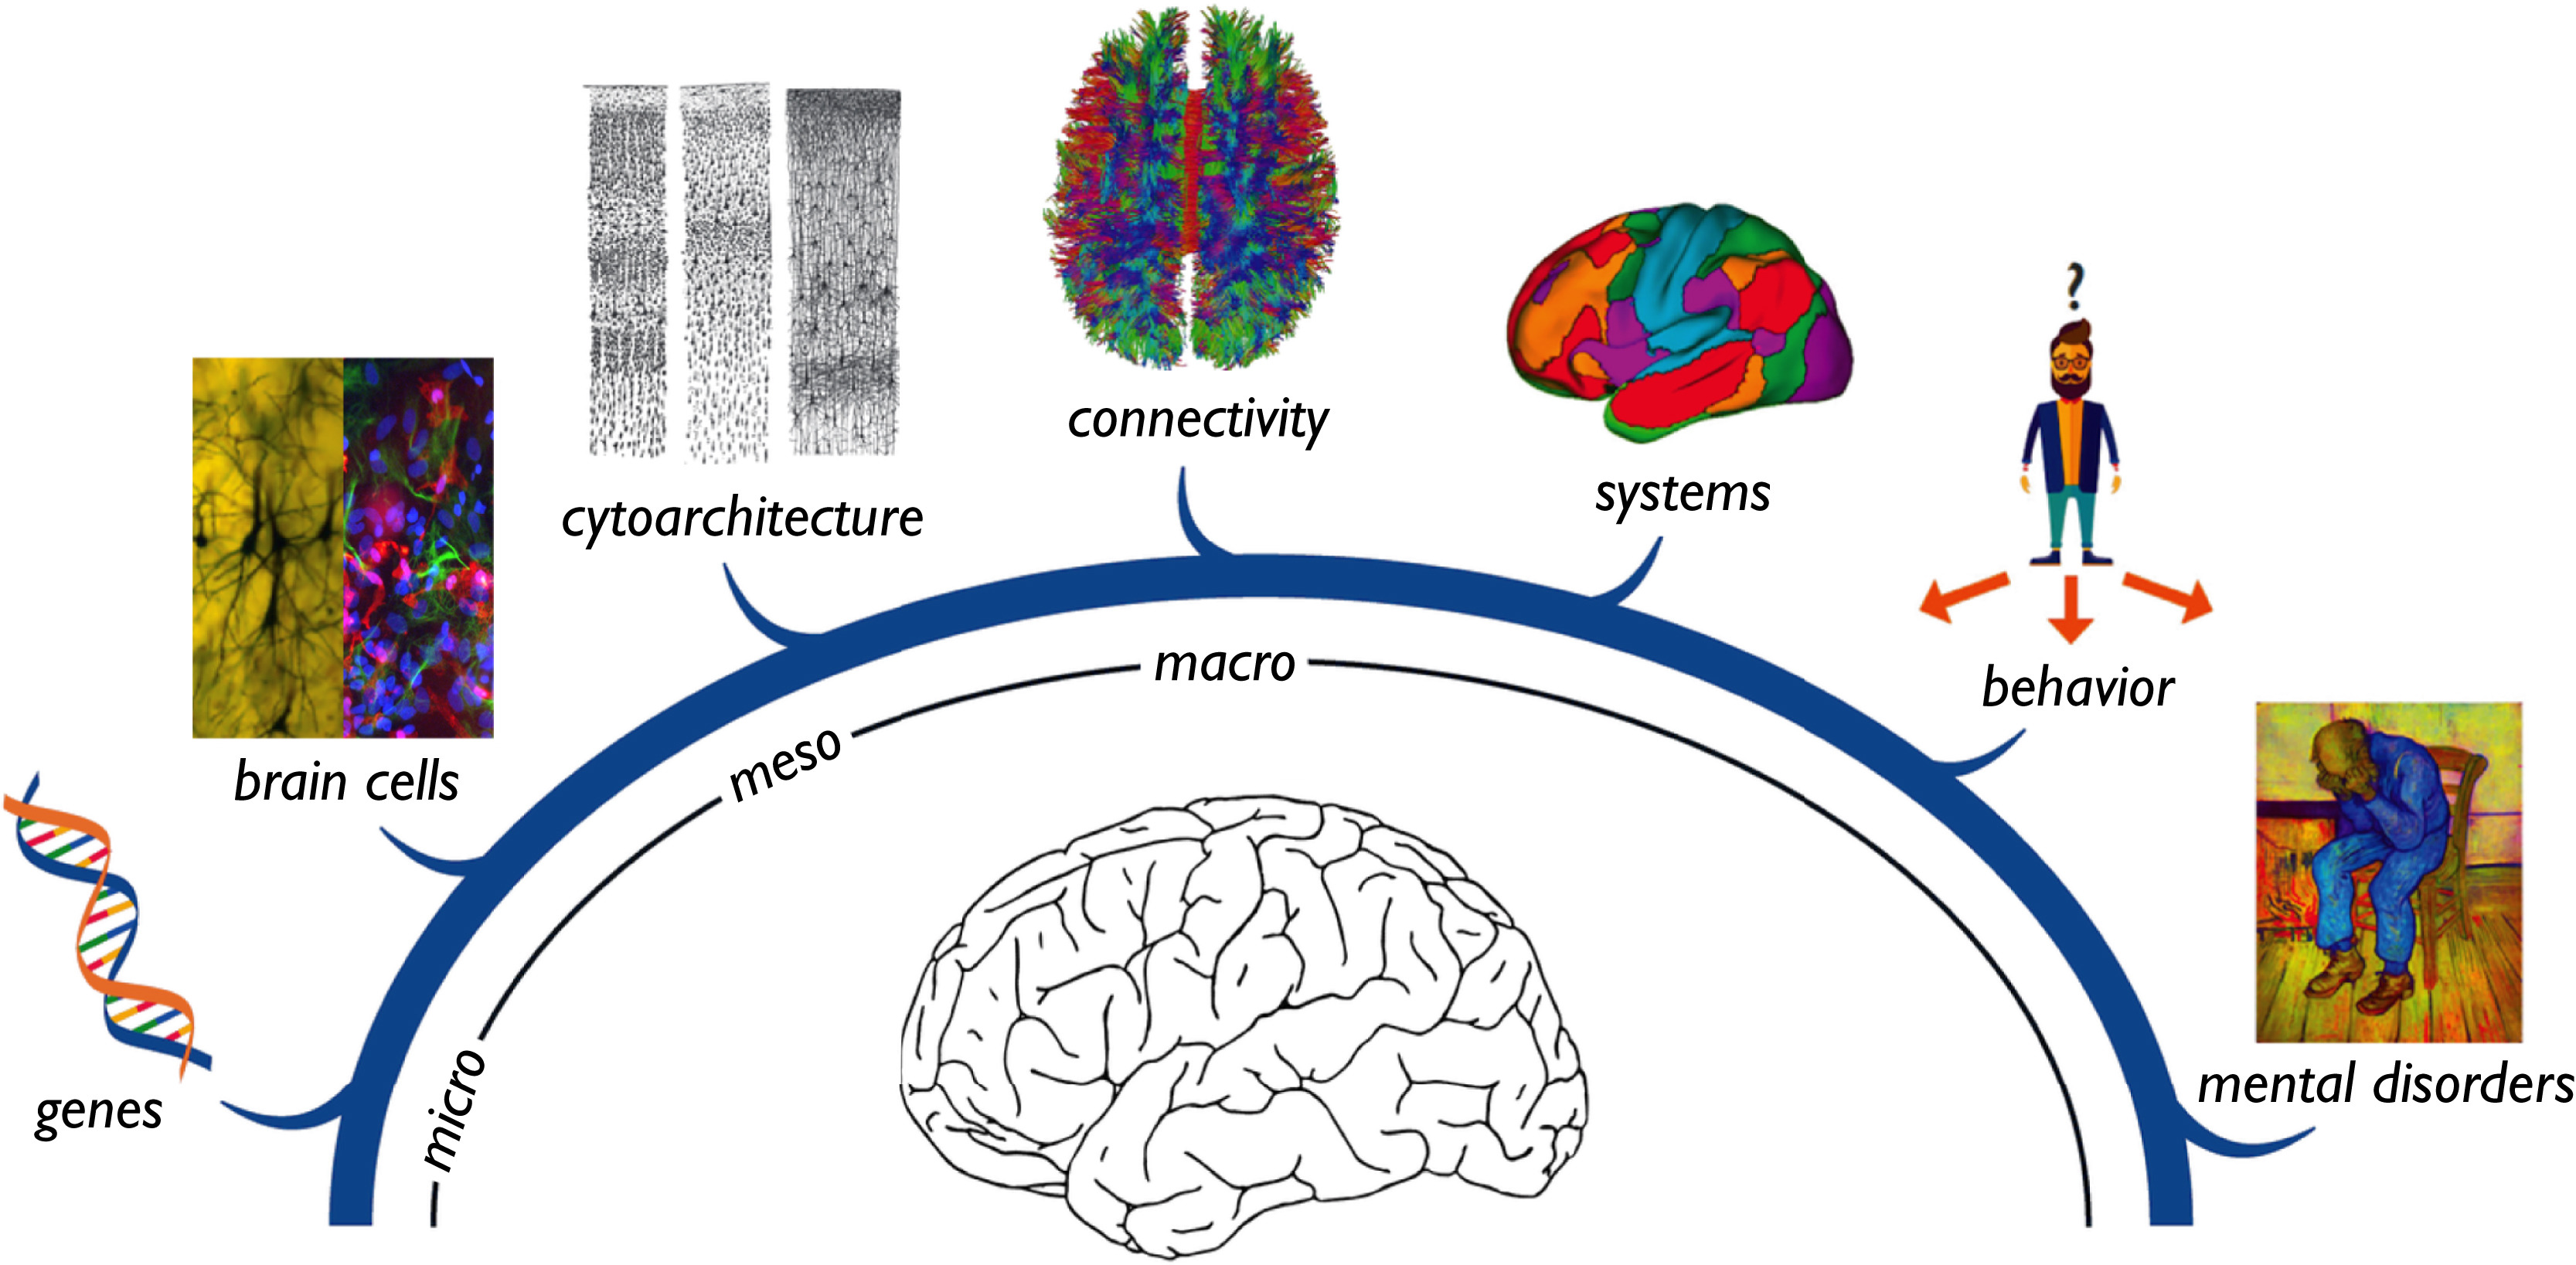
\includegraphics[width=\linewidth]{images/introFig1.jpg}
    \caption{An overview of multiscale neuroscience. The microscale, mesoscale, and macroscale human brain structure and function are integrated for an understanding of human behavior and mental disorders. Selected examples from left to right describe genes, brain cells, cytoarchitecture, connectivity, functional systems, behavior and mental disorders. Reprinted from “Multiscale Neuroscience of Psychiatric Disorders”, by Authors M.P. van den Heuvel et al., 2019, Biological Psychiatry, 86(7), 512-522. Copyright [2019] by the Society of Biological Psychiatry. Reprinted with permission.}
    \label{introFig1}
\end{figure}


\subsection*{Multiscale neuroscience and schizophrenia}
The association across different scales of brain organization can be noted not only in the healthy brain, but also in brains of patients with psychiatric disorders (Figure \ref{introFig1}). Schizophrenia is a psychiatric disorder characterized by hallucinations, delusions, a loss of initiative, cognitive dysfunction, as well as disruptions of brain connectivity \citep{Stephan2009DysconnectionIS}. Since around 100 years ago, pioneering psychiatrists Carl Wernicke (1848-1905) and Eugen Bleuler (1857-1939) hypothesized a loosening of association fibers in the brain of schizophrenia. Empirical MRI studies have provided further evidence for the widespread disruptions of interregional brain connectivity in schizophrenia \citep{EllisonWright2009MetaanalysisOD,Klauser2017WhiteMD,Fitzsimmons2013ReviewOF}, in particular disrupted connectivity between hub/rich-club regions of the brain \citep{vanDenHeuvel2013AbnormalRC,Klauser2017WhiteMD}. These alterations of hub/rich-club connectivity parallel with decreased brain network efficiency \citep{Zalesky2011DisruptedAF}, suggesting the disrupted neural information integration in schizophrenia.

A rich body of brain cytoarchitectonic studies has further shown alterations of microscale neuronal projections in schizophrenia \citep{Bakhshi2015TheNO}. For example, dendritic spines pathology has been observed in schizophrenia, in particular for layer III pyramidal neurons in prefrontal cortex, indicating disruptions of cortico-cortical and cortico-thalamus excitatory connections in schizophrenia \citep{Glausier2013DendriticSP}. Furthermore, a cross-scale study has revealed that brain regions with a more decreased spine density of pyramidal neurons showed more connectivity disruptions at the macroscale \citep{VANDENHEUVEL2016293}, confirming the macro-micro linkage in the neuropathology of schizophrenia. 

The micro-macro relationship in schizophrenia is further reflected by the underlying genetic signatures. Genome-wide association studies (GWAS) have shown that schizophrenia is a highly polygenic disorder \citep{Ripke2014BiologicalIF}, namely, a disorder led by multiple genes with additive small effects. The recent GWAS on 40,675 schizophrenia patients and 64,643 controls have identified >100 genomic risk loci and >300 risk genes \citep{Pardias2018CommonSA}. The identified genes have been shown to be associated with the formation of microscopic neuronal projection \citep{Pardias2018CommonSA}. More intriguingly, genetic variants related to risks in schizophrenia have been found to be enriched in interneuron-linked genes and can be predictive of functional activity of parvalbumin-biased brain regions \citep{Anderson2018TheTL}. Schizophrenia polygenic risk scores have shown to negatively correlate with macroscale functional connectivity in the visual network, default-mode network, and frontoparietal network \citep{Cao2020FunctionalCA}. Cortical transcriptions of schizophrenia-risk genes have also been noted to be associated with the macroscale disconnectivity pattern in schizophrenia, showing that brain regions with higher gene expression were more disconnected at the macroscale \citep{Romme2017ConnectomeDA}. 

Taken together, the genetic variants to the risk of schizophrenia, the differentiated gene expression of schizophrenia risk genes, the cellular pathological abnormalities, and the macroscale connectome alterations in schizophrenia may interactively influence each other rather than being independent. Integrating multiscale neuroscience data of schizophrenia enable us to gain a better understanding of the complex etiology of the disease.


\section*{Outline of the thesis}
This thesis aims to explore the neurobiological mechanisms underlying the human brain connectome and to scrutinize the multiscale neuropathology of schizophrenia. To do so, the following six chapters are included in this thesis. In \textbf{Chapter 2}, I use the state-of-the-art BigBrain histological dataset \citep{amunts2013bigbrain} and examine how cortical laminar cytoarchitecture relates to the organization of the macroscale brain connectome. In \textbf{Chapter 3}, I delve into the organizing principles of functional networks from the perspective of evolutionary genetics. I examine the expansion of cognitive functional networks in human evolution, and I investigate gene expression levels of human-accelerated genes (HAR genes) in those human-expanded cognitive functional networks. In addition, I demonstrate associations between human-accelerated genes and cognitive abilities and risks of psychiatric disorders in today's population based on recent GWAS results. \textbf{Chapter 4} further introduces a web-application, GAMBA, which can be used for annotating transcription-neuroimaging associations among a wide range of neuroimaging phenotypes of the healthy and diseased brain. In \textbf{Chapter 5}, I focus on schizophrenia and examine alterations of rich-club organization of the macroscale brain connectome and structural-functional connectivity coupling in first-episode, medication-naïve schizophrenia patients. In \textbf{Chapter 6}, I use magnetization transfer (MT) imaging data to provide an estimation of the microscale neuropathology in schizophrenia, and examine how microscale neuropathology correlate to macroscale dysconnectivity in schizophrenia. Finally, \textbf{Chapter 7} summarizes the findings in this thesis and discusses methodological considerations and future directions.

\printbibliography[heading=subbibliography]

\end{refsection}
% \pagestyle{MyStyle}

\chapter[Cytoarchitectonic Similarity and Brain Connectivity]{Multiscale Examination of Cytoarchitectonic Similarity and Human Brain Connectivity}
\label{ch:fourthpaper}

\begin{refsection}


\begin{FlushRight}
\textit{Yongbin Wei, Lianne H. Scholtens, Elise Turk, Martijn P. van den Heuvel}\\
Network Neuroscience, 2018; 3(1): 124-137

\end{FlushRight}
\vspace{20pt}

\newpage
\section*{Abstract}
The human brain comprises an efficient communication network, with its macro-scale connectome organization argued to be directly associated with the underlying microscale organization of the cortex. Here, we further examine this link in the human brain cortex by using the ultrahigh resolution BigBrain dataset. 11,660 BigBrain profiles of laminar cell structure were extracted from the BigBrain data and mapped to the MRI based Desikan-Killiany atlas used for macroscale connectome reconstruction. Macroscale brain connectivity was reconstructed based on the diffusion weighted imaging dataset from the Human Connectome Project and cross-correlated to the similarity of laminar profiles. We showed that the BigBrain profile similarity between interconnected cortical regions was significantly higher than those between non-connected regions. The pattern of BigBrain profile similarity across the entire cortex was also found to be strongly correlated with the pattern of cortico-cortical connectivity at the macroscale. Our findings suggest that cortical regions with higher similarity in the laminar cytoarchitectonic patterns have higher chance of being connected, extending the evidence for the linkage between macroscale connectome organization and microscale cytoarchitecture.

\section*{Introduction}
The human brain connectome is a comprehensive map comprising interconnections of neural elements at multiple scales \citep{sporns_human_2005,sporns_human_2011}. At the microscale, neuron-to-neuron connections are formed by axons, dendrites, and synapses, processing and transmitting neural information by means of electrical and chemical signals \citep{cossell_functional_2015,yuste_dendritic_2011,ullo_functional_2014}. In parallel, the macroscale connectome consists of cortical regions that are linked by large scale white matter tracts, providing a structural backbone supporting functional specialization and efficient information integration \citep{bullmore_economy_2012,van_den_heuvel_network_2013}.

In recent years, studies have aimed to bridge these two levels of brain organization, and have suggested that macroscale brain connectivity might be indeed associated with cortical cytoarchitecture patterns. The large variety in cytoarchitecture across the human cerebral cortex \citep{brodmann1909vergleichende,von1925cytoarchitektonik} has been suggested to yield a rich body of cortical circuit patterns for diverse functions, with, for example, larger and more spinous pyramidal cells observed in prefrontal cortex compared with primary regions (e.g., visual cortex; \citep{elston2003cortex,elston2001pyramidal}. Expanding the thoughts of cytoarchitectonic variation, studies have further proposed that the interareal cytoarchitectonic differentiation plays a pivotal role in shaping cortico-cortical connections \citep{barbas2015general}. Moreover, modern human and animal connectome studies have also provided quantitative evidence for the relation between brain connectivity and cortical cytoarchitecture. Highly connected cortical regions have layer III pyramidal cells with large basal dendritic tree size, a large number of spines per neuron in the macaque brain \citep{scholtens2014linking}, and large neuron soma size in the human brain \citep{van2015bridging}. The presence or absence of interregional connectivity has also been observed to be associated with the cortical cytoarchitectonic differentiation, showing that regions with more similar cytoarchitecture type had a greater chance to be connected \citep{beul2017predictive,beul2015predictive,goulas2016cytoarchitectonic,goulas2017principles,hilgetag2016primate}.

Recently, an ultrahigh-resolution three-dimensional model of a cell body–stained human brain was provided by \citet{amunts2013bigbrain}; 7,404 histological sections were collected from a complete paraffin-embedded brain at a nearly cellular resolution of 20 micrometers, resulting in the BigBrain dataset. The BigBrain provides higher sampling rate within the whole brain and allows direct mapping to the modern neuroimaging data. Therefore, it can serve as a good quantitative reference to link macroscale in vivo brain mapping findings to microscale cytoarchitecture in the human cerebral cortex. In the current study, we used the BigBrain dataset and sought to examine how the cortical cytoarchitecture shapes the large-scale connectivity in human brain. We combined the information on cortical layer composition extracted from the BigBrain images with the diffusion-weighted imaging (DWI) data from the Human Connectome Project \citep{VANESSEN201362}. Linking BigBrain profile similarity to the reconstructed macroscale connectome, we extend evidence for the association between microscale cytoarchitectonic similarity and macroscale connectome organization in the human brain.

\section*{Methods}
\subsection*{BigBrain Data}
As described in detail by \citet{amunts2013bigbrain}, the BigBrain data includes 7,404 histological sections with 20-$\mu$m thickness that were cut in coronal plane from a complete postmortem paraffin-embedded human brain of a 65-year-old man without any neurological or psychiatric diseases in clinical records. All sections were stained for cell bodies \citep{MERKER1983235} and were digitized into high-resolution images of 13,000 $\times$ 11,000 pixels (10 $\times$ 10 $\mu$m$^{2}$). The digitized images were downsampled to 20 $\times$ 20 $\mu$m$^{2}$ to obtain an isotropic resolution matching the slice thickness of 20 mm. Defects of histological artifacts, such as rips, tears, folds, missing and displaced pieces, distortion (shear), stain inhomogeneity, and crystallization, were repaired both manually and automatically to restore the integrity of all slices \citep{amunts2013bigbrain}. All preprocessed images were downloaded in PNG format from http://bigbrain.loris.ca/main.php.

\subsubsection*{BigBrain Profiles}
Using the BigBrain dataset, we extracted cortical profiles that delineate the laminar cell number and density of the cortex. Resulting BigBrain profiles were extracted according to the following steps. First, 11,660 pairs of points on the cortex boundaries were manually selected from BigBrain images. During the selection, random image sections were chosen and four pairs of points were selected with short intervals. For each pair of points, the first point was selected on the pial surface and the second on the white matter surface (Figure \ref{bigbrainFig1}), forming a line segment perpendicular to the two surfaces. Second, we searched the closest neighbor pair for each pair of points according to the Euclidean distance. Linking each pair of points and their nearest neighbor formed a quadrilateral in the image that covered a small cortical area. Inside the quadrilateral, we uniformly sampled 1,000 blocks from the pial surface to the white matter surface. The mean image intensity of each block was computed to reflect the level of cell size and density within the block (because images were cell body stained). A curve of image intensities was subsequently generated for each pair of points and named the BigBrain profile (Figure \ref{bigbrainFig1}). The resulting BigBrain profiles were found to be comparable with profiles based on the histological information derived from the von Economo and Koskinas atlas; see Supporting Information, \citet{WEI2019bigbrain}). All procedures were implemented in MATLAB.

\begin{figure}[h]
  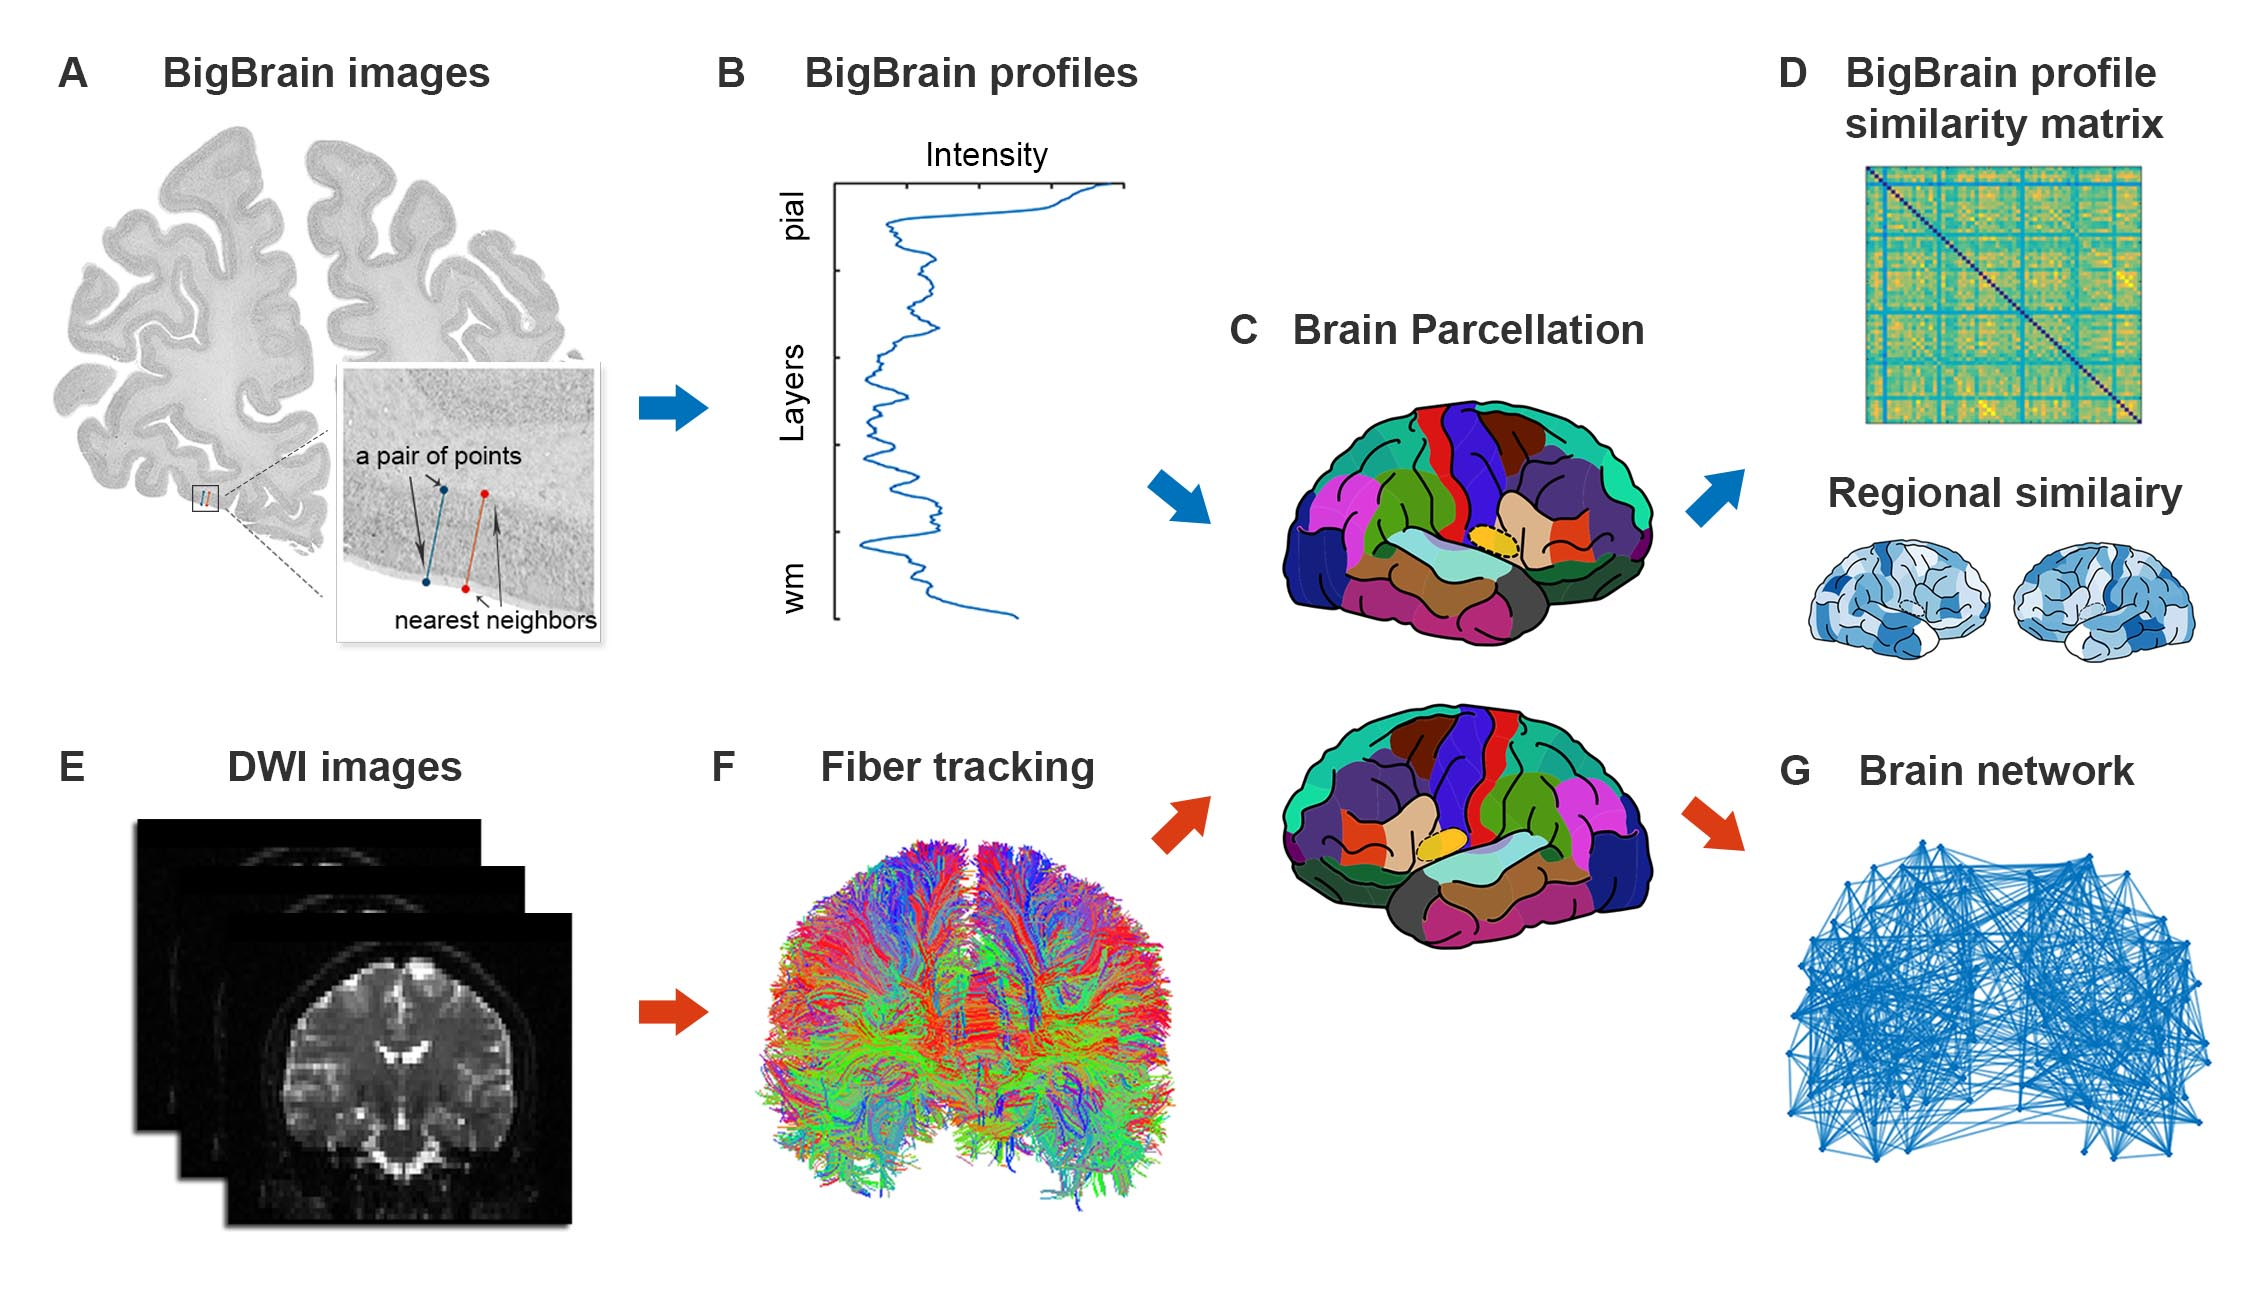
\includegraphics[width=\linewidth]{images/thesis_bb_fig1.jpg}
  \caption{Overview of the data processing steps. (A) An example of a BigBrain image, selected pair of points, and its closest neighbor pair. (B) A manual BigBrain profile was extracted from the BigBrain image according to randomly selected points. (C) BigBrain profile was registered to the Desikan–Killiany atlas and averaged within each cortical region. (D) The average BigBrain profiles were correlated between every two cortical regions to obtain a similarity matrix. In parallel, we used DWI data (E) and performed fiber tracking (F) to reconstruct the brain structural network (G). BigBrain profile similarity was linked to properties of the brain structural network.}
  \label{bigbrainFig1}
\end{figure}

\subsubsection*{Anatomical registration}
BigBrain profiles were registered to a common space of MRI data for further region-wise analyses. First, BigBrain images (i.e., PNG files) were transformed to NIfTI format, forming a customized BigBrain image, and resampled to a resolution of 400 $\mu$m to optimize computation time. Second, we registered the BigBrain image to the reference brain volume in the Montreal Neurological Institute (MNI) International Consortium of Brain Mapping (ICBM) 152 space (downloaded from https://bigbrain.loris.ca/), by applying the affine registration tool FLIRT \citep{JENKINSON2001143,JENKINSON2002825} followed by a nonlinear registration using FNIRT tools \citep{Andersson2007NonlinearOF}, employing a b-spline representation of the registration warp field (Supporting Information Figure S1, \citet{WEI2019bigbrain}). Third, brain parcellations in the FreeSurfer fsaverage template were affine registered to the MNI ICBM 152 space by using FLIRT, followed by warping to the customized BigBrain image by using the inversed registration warp field generated in the second step (Supporting Information Figure S1, \citep{WEI2019bigbrain}). Brain parcellations included (a) the 68-region Desikan-Killiany (DK) atlas \citep{DESIKAN2006968,Fischl2004parcellation}, which was used in the main results, and (b) the 114-region DK subdivision \citep{CAMMOUN2012386}, and (c) the von Economo–Koskinas (EK) atlas \citep{Scholtens2015ECONOMO,SCHOLTENS2018ECONOMO,von1925cytoarchitektonik} for validation purposes. Fourth, given the coordinates of the point pairs (which were used to extract BigBrain profiles) in the BigBrain images, we searched for their nearest voxels in the customized BigBrain image. This way, each BigBrain profile was assigned to the DK region that its nearest voxel belongs to, making it possible to obtain the regional BigBrain measurements in the original BigBrain space; 2,438 BigBrain profiles located too far from the nearest cortical voxel (>1.5 interquartile range [IQR] distance to the nearest cortical voxel) were excluded as outliers. Four hundred thirteen BigBrain profiles crossing DK region boundaries — with the nearest neighbor point-pair located in a different DK region — were further excluded to avoid samples at boundaries. As a result, 8,809 BigBrain profiles were included in further analyses.

\subsection*{BigBrain Profile Similarity}
A regional BigBrain profile was obtained per region by averaging BigBrain profiles within the region. A mean number of 133 profiles (standard deviation [SD]: 158) was included per DK region. Eight DK regions with fewer than 20 profiles were excluded from further analyses because of the possible bias resulting from an insufficient number of samples. We noted that adopting additional thresholds of 0 and 50 profiles to examine the possible effect of small regions revealed similar findings (see Supporting Information, \citet{WEI2019bigbrain}). Next, a matrix of interregional similarity of BigBrain profiles was obtained by calculating the Pearson’s correlation between the regional BigBrain profiles of every pair of DK cortical areas. The resulting profile similarities were observed to demonstrate a non-normal distribution and were transformed to a normal distribution with mean of 1 and SD of 0.2 by matching ranks. Using the raw similarity (i.e., non-redistributed data) showed similar results (see Supporting Information, \citet{WEI2019bigbrain}). For regional analysis, values of each column within the matrix were averaged, resulting in a vector representing the mean similarity level of a region to the rest of the brain.

\subsection*{MRI Data}
High-quality T1-weighted MRI data and diffusion-weighted MRI data from 215 subjects (age [mean $\pm$ SD]: 29.8 $\pm$ 3.4 years old) from the Q3 data release of the Human Connectome Project were used in the current study \citep{VANESSEN201362}. The FreeSurfer software package \citep{FISCHL2012Freesurfer} was used to obtain brain tissue segmentation and cortical mantle reconstruction from the T1-weighted data. The DK atlas was used for cortical parcellation \citep{DESIKAN2006968,Fischl2004parcellation}.

White matter tracts were reconstructed from DWI images by using the following procedure \citep{VANDENHEUVEL2016293}. First, the 18 sets of b = 0 volumes were averaged, and the 270 diffusion images were realigned and corrected for small head motions and common gradient-induced distortions \citep{ANDERSSON2002177}. Second, the diffusion profile within each voxel was reconstructed using generalized q-sampling imaging, allowing for reconstruction of crossing fibers \citep{YEH2010}. Third, deterministic tractography was performed to reconstruct white matter tracts, performing fiber assignment by using the Fiber Assignment by Continuous Tracking (FACT) algorithm \citep{MORI1999}. For each voxel, eight streamline seeds were started and tracking was stopped if the streamline reached a voxel of low preferred diffusion direction (fractional anisotropy < 0.1), exited the gray matter/white matter mask, or made a sharp turn (>45$^{\circ}$).

\subsection*{Connectome Construction}
A structural network was constructed from the set of reconstructed tractography streamlines and the cortical parcellation for each subject. Here, network nodes were defined as cortical regions, and edges were placed between nodes that were connected by reconstructed streamlines. The number of reconstructed streamlines (NOS) was used to weight network edges. NOS was transformed to a normal distribution (mean = 1, SD = 0.2). Moreover, streamline density of each edge was obtained by dividing NOS by the mean volume of the two connected regions, and also used as a connection weight. A group-averaged binary network was formed by placing an edge between two brain regions if those regions were connected in more than 50\% of the subjects. Alternative thresholds of >40\% and >60\% were used as validations (see Supporting Information, \citet{WEI2019bigbrain}). The weighted network was obtained by averaging nonzero weights (i.e., NOS and streamline density) of each edge in the group binary network across all subjects.

\subsection*{Connectome Analyses}
Graph theoretical analyses were conducted on the reconstructed structural network. Four nodal metrics were calculated on both the group binary and the group-weighted networks, including nodal degree/strength (for the binary/weighted network, respectively), betweenness centrality, clustering coefficient, and mean path length. First, degree was computed for each node as the number of edges connected to a node. Likewise, nodal strength was obtained by taking the sum of weights of edges connected to a node. Second, betweenness centrality was calculated as the fraction of all shortest paths in the network that traverse a given node, where the shortest path length was defined as the lowest number of edges that must be traversed to go from one node to the other. The obtained betweenness centrality values were found to be nonnormally distributed and were thus log transformed. Third, the clustering coefficient for each node was computed as the proportion of edges between the node’s neighbors divided by the number of edges that could possibly exist between these neighbors. Finally, the mean path length was obtained for each node by averaging the shortest path length between this node and the rest of the nodes in the network. Graph metrics were computed using the brain connectivity toolbox (https://sites.google.com/site/bctnet/; \citet{RUBINOV20101059}).


\subsection*{Statistical Analysis}
A two-tailed two-sample \textit{t} test was used to investigate the difference of BigBrain profile similarity between interconnected cortical regions and nonconnected cortical regions. Pearson’s correlation analysis was performed to estimate the association of BigBrain profile similarity with connection weights in the group-weighted structural network. Analyses were reperformed for connections within left and right hemisphere, and between hemispheres, separately. Moreover, regional BigBrain profile similarity was correlated to the nodal degree/strength, clustering coefficient, path length, and betweenness centrality of the group-averaged connectome map. We also conducted a partial correlation between the regional BigBrain profile similarity level and nodal graph metrics by taking the number of individual BigBrain profiles per region as covariates to investigate the influence of the sample size of BigBrain profiles. To examine the dependency among graph metrics, multiple linear regression was performed as:

\[\mathsf{Y=\beta_0+\beta_1X_1+\beta_2X_2+\beta_3X_3+\beta_4X_4+\epsilon}\]

with \textit{Y} indicating the BigBrain profile similarity and \textit{X}$_1$, …, \textit{X}$_4$ nodal strength, betweenness centrality, clustering coefficient, and shortest path length, respectively, and with $\beta_i$ representing coefficients and $\epsilon$ the residuals. For all above analyses, effects reaching a false discovery ratio (FDR) corrected \textit{q} < 0.05 (across all 28 tests done in the main result) were taken as significant.

\subsection*{Interregional Distance}
As discussed by recent studies \citep{beul2017predictive,beul2015predictive}, interregional distance may play an important role in the organization of brain connectivity. Here, we also examined whether the physical distance between brain regions influenced BigBrain profile similarity and its association with connectivity. First, we calculated the coordinates of centroids of each DK region in the FreeSurfer fsaverage template by averaging the (X, Y, Z) coordinates of all voxels within a region. Second, the Euclidean distance between centroids of DK regions was computed and taken as the interregional physical distance. Third, connections were divided into three categories according to the distance ranking, including short-range (top 25\% shortest connections), long-range (top 25\% longest connections), and mid-range connections (others). The BigBrain similarity difference across three connectivity categories was examined using one-way ANOVA analysis and post hoc two-sample t tests. Finally, interregional distance, together with the mean cortical volume and surface area (i.e., the mean volume and surface area between every cortical region pair), were regressed out from both BigBrain profile similarity and connectivity strength, separately, by using linear regression. Residuals were used to reevaluate the association of BigBrain profile similarity with connectivity.

\subsection*{Validation Analyses Using von Economo–Koskinas Data}
The EK data was used to examine the agreement of our BigBrain profiles with classical measurements. In 1925, Constantin von Economo and George Koskinas published a comprehensive brain atlas comprising 48 “most important” distinct cortical areas as well as detailed layer-specific histological information on neuronal count, neuron size, and cortical thickness \citep{von1925cytoarchitektonik}. A digital version of the EK atlas based on the FreeSurfer Software \citep{FISCHL2012Freesurfer} was used to link the historical histology data to modern anatomical imaging \citep{SCHOLTENS2018ECONOMO,Scholtens2015ECONOMO}. We mapped BigBrain profiles to the EK atlas and computed the regional averaged mean and SD of BigBrain profiles. Additionally, the length of the line segment formed by each pair of points was recorded as an assessment of cortical thickness. In parallel, EK profiles were generated for each EK area by sampling 1,000 steps from the pial to the white matter surface and for each step assigning the corresponding layers’ (neuron density $\times$ neuron size) value \citep{von1925cytoarchitektonik}. The mean and SD of the resulting EK profiles were also computed. Pearson’s correlation was used to estimate the similarity of BigBrain profile with EK profiles and the agreements of properties (i.e., mean and SD) of the two types of profiles (see Supporting Information, \citet{WEI2019bigbrain}).

\section*{Results}
BigBrain profile similarity between interconnected cortical regions was observed to be significantly higher than between nonconnected regions (\tvaldf(1,709) = 9.36, \pval < 0.0001, FDR corrected; Figure \ref{bigbrainFig2}C), suggesting that regions with higher cytoarchitectonic similarity were more likely to be connected. With respect to all connected regions, BigBrain profile similarity was significantly correlated with connection strength of the group structural network (NOS: \rval = 0.28, 
\pval < 0.0001; streamline density: \rval = 0.17, \pval = 0.0003, FDR corrected; Figure \ref{bigbrainFig2}D), which indicates that cortical regions showing higher cytoarchitectonic similarity have a higher probability of being linked by stronger white matter connections.

\begin{figure}[h]
    \centering
    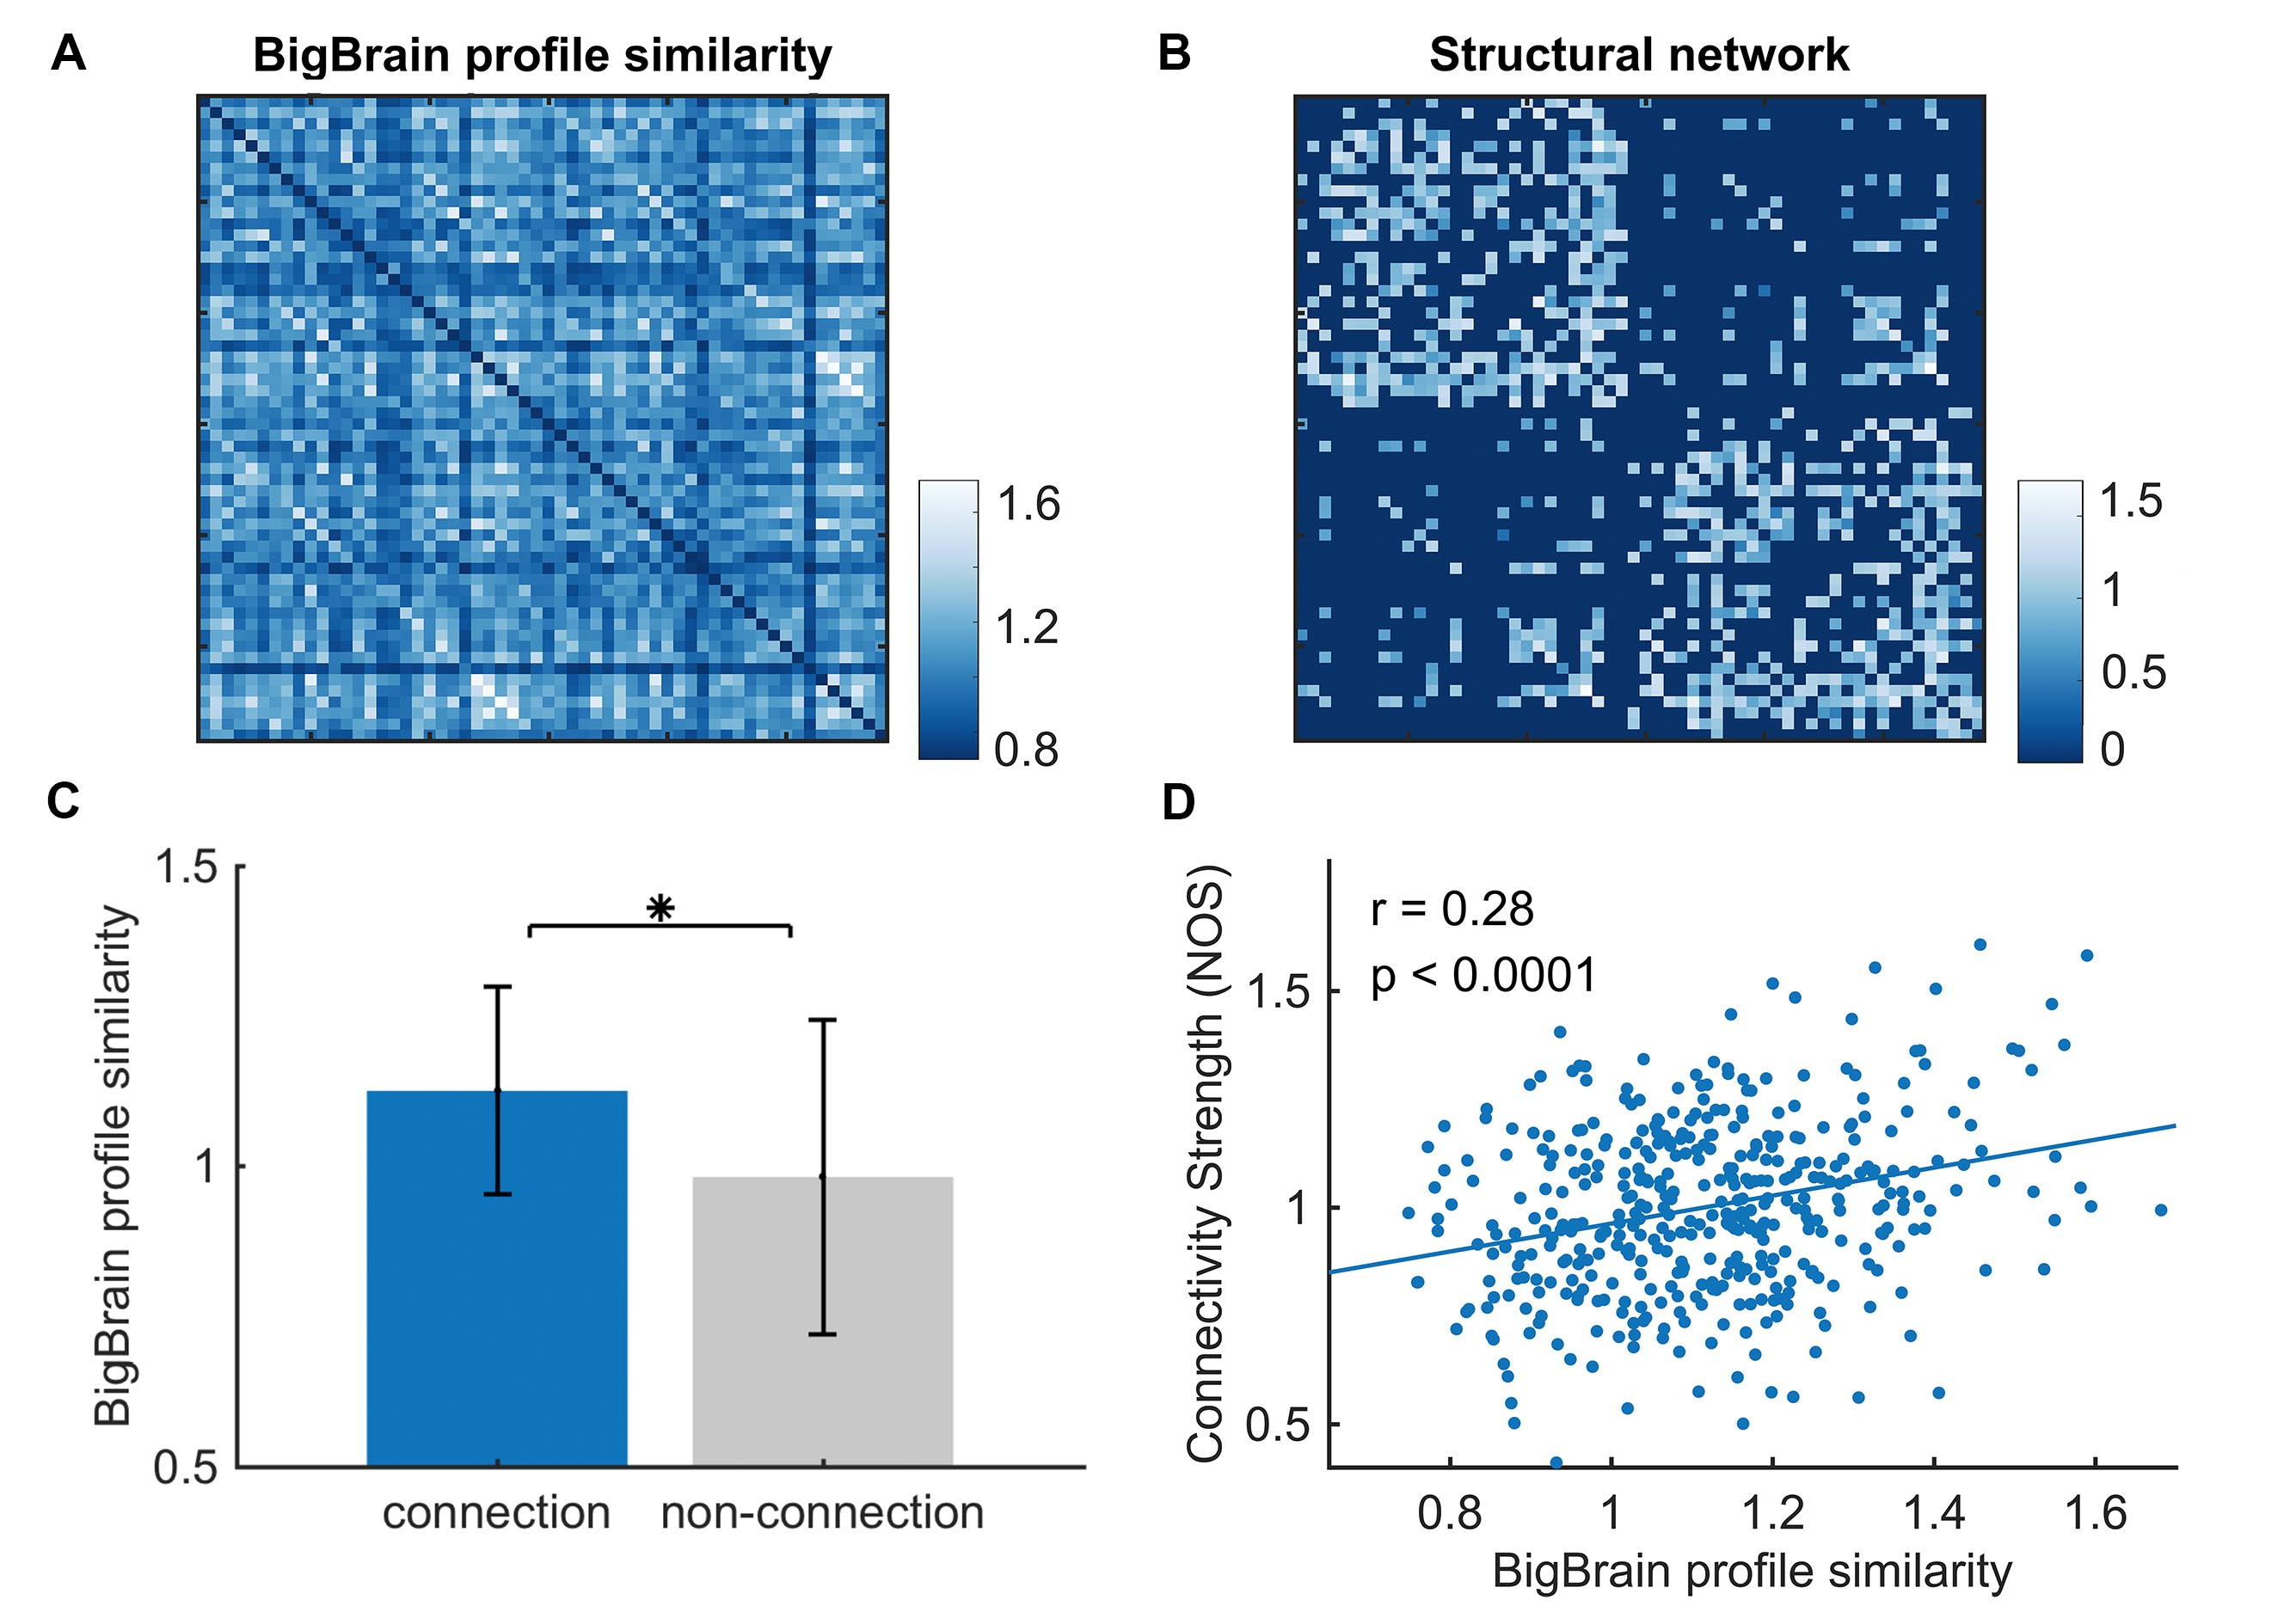
\includegraphics[width=\linewidth]{images/thesis_bb_fig2.jpg}
    \caption{Association of BigBrain profile similarity with structural connectivity at the edge-level. (A) BigBrain profile similarity matrix. (B) Group-weighted structural connectivity matrix. (C) BigBrain profile similarity between interconnected regions was significantly higher than between nonconnected regions (\tvaldf(1,709) = 9.36, \pval < 0.0001). (D) BigBrain profile similarity was positively correlated with connection weight (NOS) of the structural network (\rval = 0.28, \pval < 0.0001).}
    \label{bigbrainFig2}
\end{figure}

Considering the interregional distance, we observed a significant difference for BigBrain profile similarity across short-, mid-, and long-range connections (\textit{F}(389) = 9.75, \pval < 0.0001, FDR corrected), showing the highest similarity for short-range connections and the lowest for long-range connections (Figure \ref{bigbrainFig3}A). Notably, BigBrain profile similarity showed correlations with connectivity strength for each subset of connections: short-range (\rval = 0.30, \pval = 0.0032), mid-range (\rval = 0.16, \pval = 0.0245), and long-range connectivity (\rval = 0.32, \pval = 0.0014, all FDR corrected). We further regressed out this effect, together with the effect of cortical area size, from the BigBrain profile similarity and reevaluated the observed association of profile similarity to cortico-cortical connectivity. Residuals of BigBrain profile similarity remained to be larger between interconnected regions than nonconnected regions (\tvaldf(1,709) = 10.14, \pval < 0.0001, FDR corrected). The correlation between profile similarity and connectivity strength also persisted (\rval = 0.27, \pval < 0.0001, FDR corrected; Figure \ref{bigbrainFig3}B).

\begin{figure}[h]
    \centering
    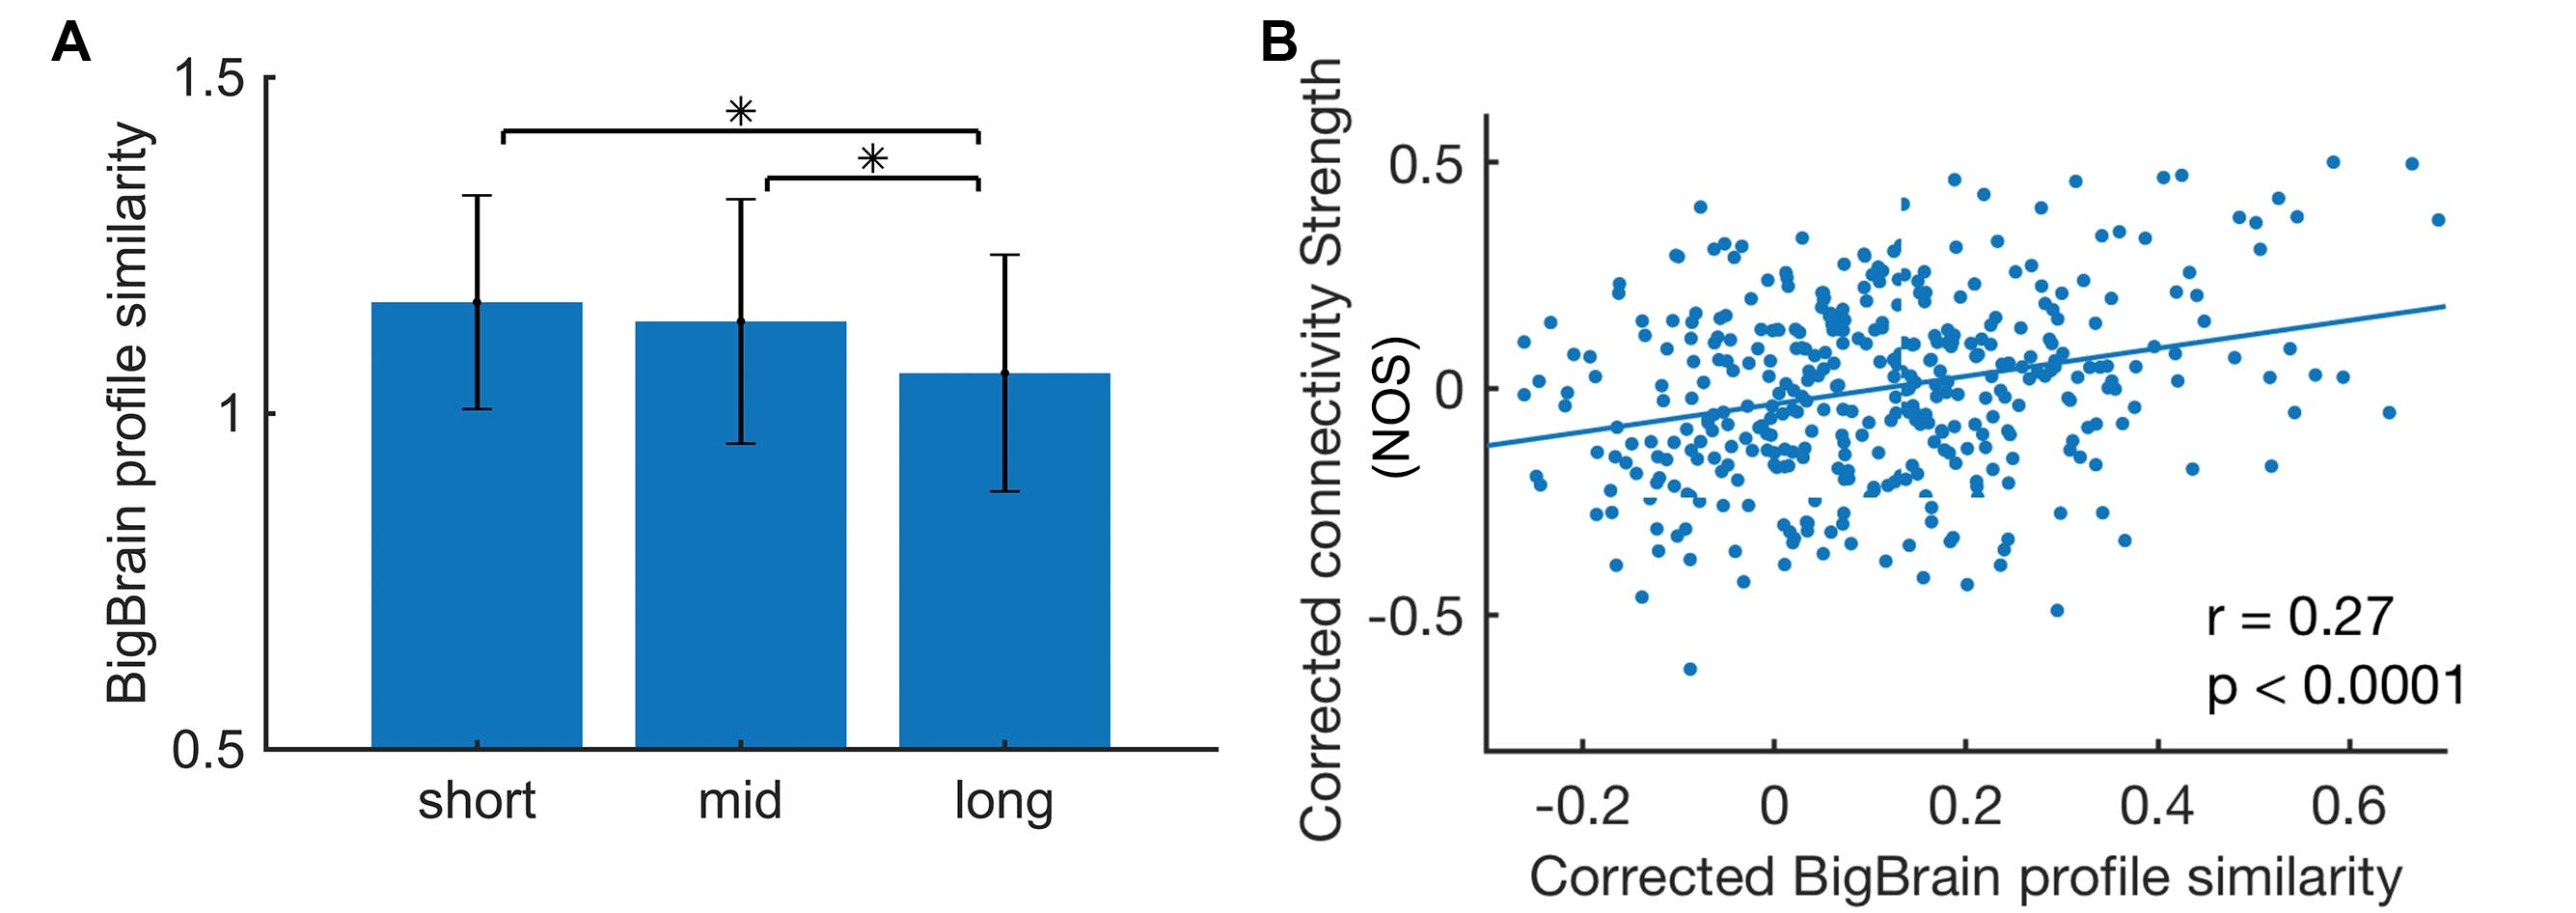
\includegraphics[width=\linewidth]{images/thesis_bb_fig3.jpg}
    \caption{BigBrain profile similarity and interregional distance. (A) BigBrain profile similarity was different among short-, mid-, and long-range connections (\textit{F}(389) = 9.75, \pval < 0.0001). Short-range connections showed significantly higher profile similarity than mid- (\tval = 3.42, \pval = 0.0007) and long-range connections (\tval = 4.34, \pval < 0.0001). (B) Regressing out interregional distance and the mean regional volume and surface area, BigBrain profile similarity still correlated with the connectivity strength (\rval = 0.27, \pval < 0.0001).}
    \label{bigbrainFig3}
\end{figure}

The association between BigBrain profile similarity and connectivity was further examined in context of intra- and interhemispheric connections. BigBrain profile similarity was found to be higher in connected regions than nonconnected regions within the left hemisphere (\tvaldf(376) = 5.37, \pval < 0.0001, FDR corrected) and right hemisphere (\tvaldf(433) = 7.19, \pval < 0.0001, FDR corrected), as well as between interhemisphere connected and nonconnected regions (\tvaldf(838) = 7.54, \pval < 0.0001, FDR corrected; Figure \ref{bigbrainFig4}A). Taking within-hemisphere and interhemisphere connections separately, BigBrain profile similarity consistently showed a significant correlation with the connection strength (\rval = 0.32 and $0.23$ for connections in left and right hemisphere, and \rval = 0.47 for interhemispheric connections, all \pval < 0.0001, FDR corrected; Figure \ref{bigbrainFig4}B).

\begin{figure}[h]
    \centering
    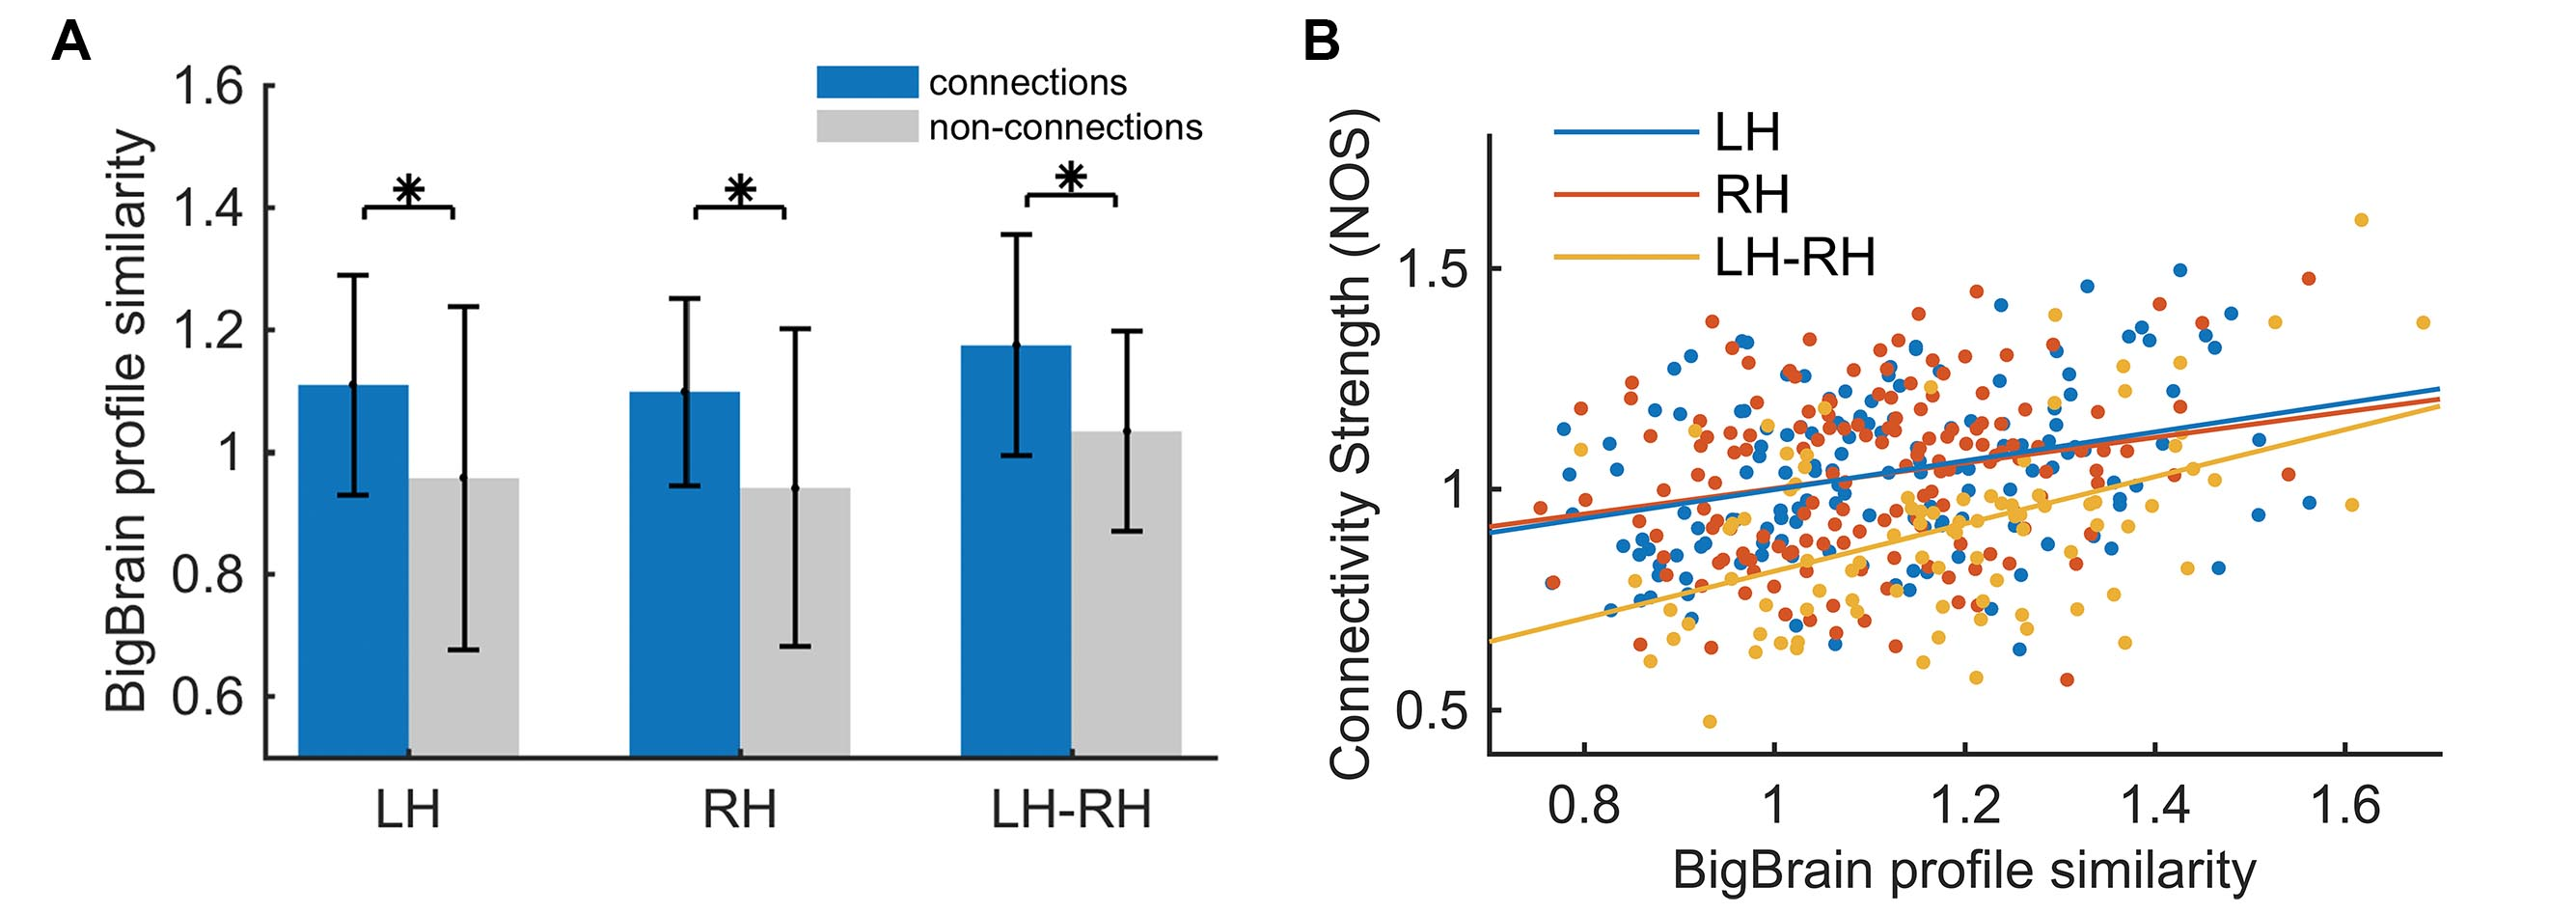
\includegraphics[width=\linewidth]{images/thesis_bb_fig4.jpg}
    \caption{BigBrain profile similarity and inter-/intra-hemispheric connections. (A) Both intra- and interhemispheric BigBrain profile similarity was higher between connected regions compared with nonconnected regions (Left hemisphere [LH]: \tvaldf(376) = 5.37, \pval < 0.0001; right hemisphere [RH]: \tvaldf(433) = 7.19, \pval < 0.0001; interhemisphere [LH-RH]: \tvaldf(838) = 7.54, \pval < 0.0001). (B) Taking LH, RH, and LH-RH connections separately, BigBrain profile similarity consistently showed correlations with connection strength (\rval = 0.32, 0.23, and 0.47, separately, all \pval < 0.0001; *significant differences).}
    \label{bigbrainFig4}
\end{figure}

Correlating the pattern of regional BigBrain profile similarity to nodal strength of the group structural network showed a significant correlation (NOS: \rval = 0.56, \pval < 0.0001; streamline density: \rval = 0.37, \pval = 0.0042, FDR corrected; Figure \ref{bigbrainFig5}), confirming that regions with higher BigBrain profile similarity to the rest of regions tend to be connected by stronger connections at the macroscale level. Correlation analysis between regional BigBrain profile similarity and nodal degree of the group binary network demonstrated similar results (\rval = 0.52, \pval < 0.0001, FDR corrected). Findings persisted when we examined the partial correlation between BigBrain profile similarity and macroscale nodal degree/strength by taking the number of BigBrain profiles of each cortical region as covariates (\(\rho\) = 0.45, \pval = 0.0004 for the strength; \(\rho\) = 0.38, \pval = 0.0035 for the degree, FDR corrected). Regressing out the interregional distance from BigBrain profile similarity and connectivity strength (NOS) revealed a similar correlation (\rval = 0.41, \pval = 0.0014, FDR corrected).

\begin{figure}[h]
    \centering
    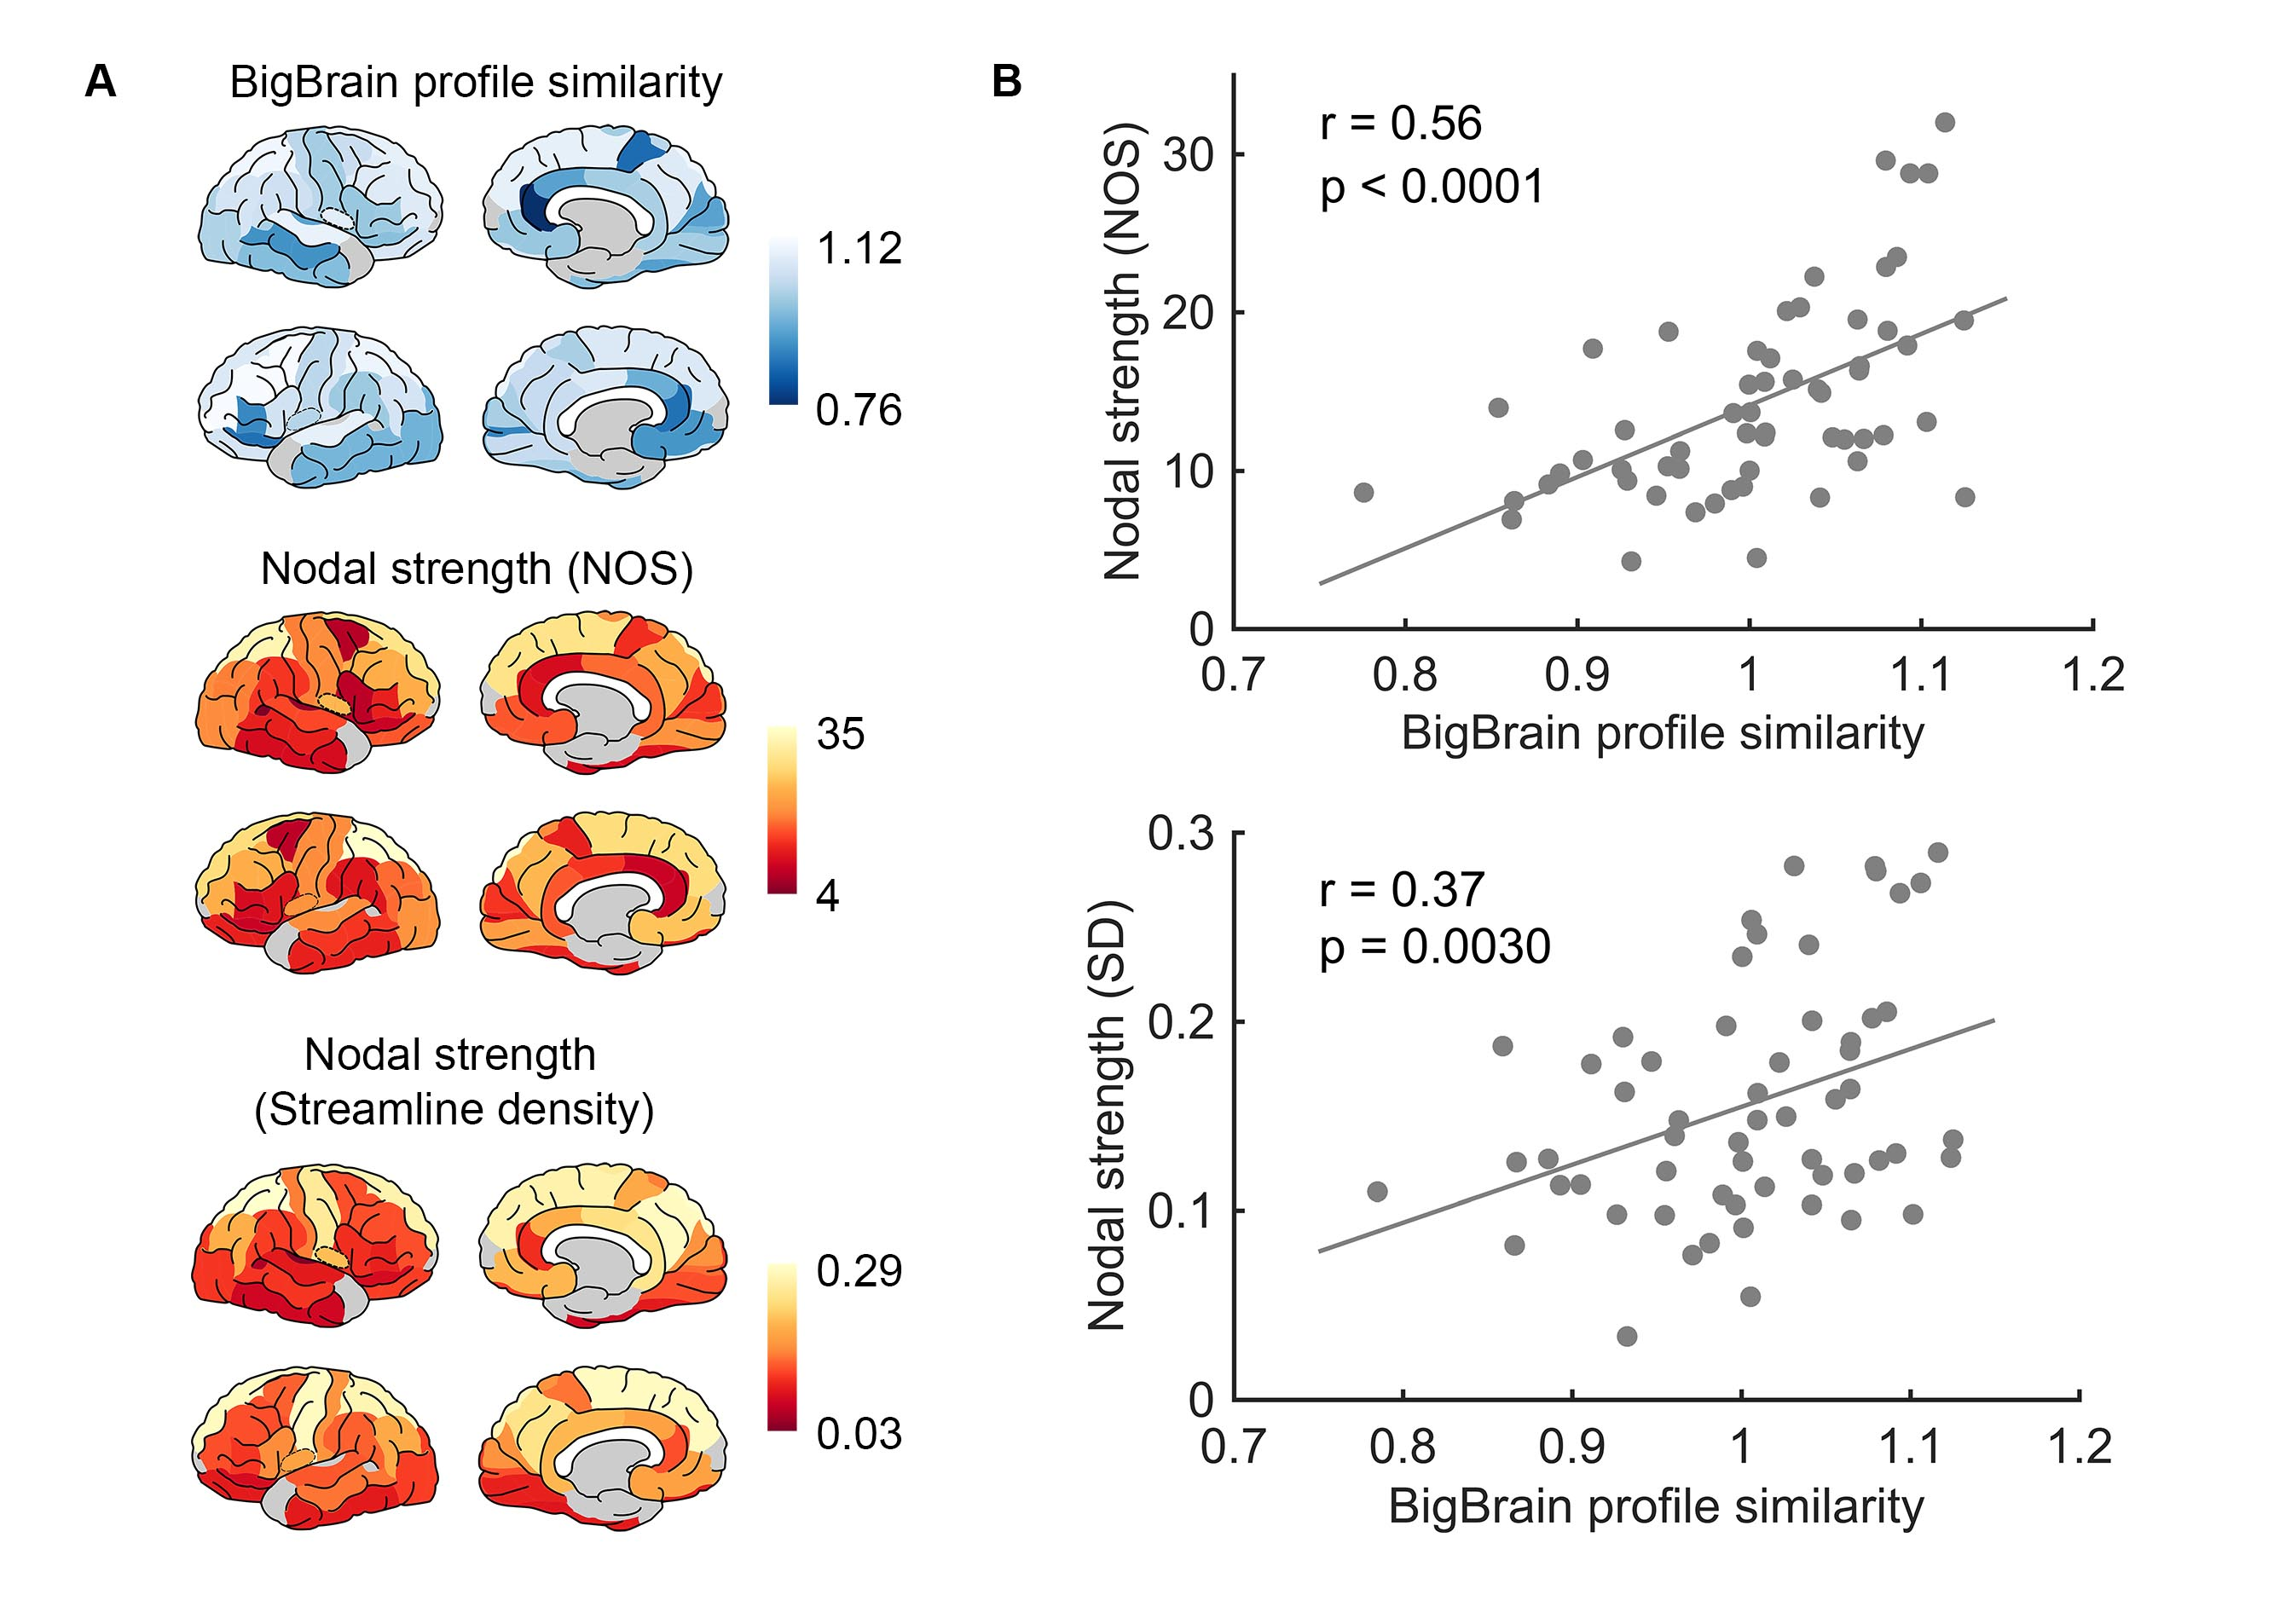
\includegraphics[width=\linewidth]{images/thesis_bb_fig5.jpg}
    \caption{BigBrain profile similarity and connectivity at the nodal-level. (A) The pattern of regional BigBrain profile similarity (top) and nodal strength (middle: NOS weights; bottom: streamline density weights). (B) Regional BigBrain profile similarity showed significant correlation with nodal strength (top: NOS, \rval = 0.56, \pval < 0.0001; bottom: streamline density, \rval = 0.37, \pval = 0.0030).}
    \label{bigbrainFig5}
\end{figure}

Regional BigBrain profile similarity was significantly correlated with betweenness centrality (NOS,\rval = 0.44, \pval = 0.0033, FDR corrected; Figure \ref{figure4:graph}). Meanwhile, negative associations were found with clustering coefficient (\rval = -0.35, \pval = 0.0070, FDR corrected) and mean shortest path length (\rval = -0.50, \pval = 0.0001, FDR corrected; Figure \ref{figure4:graph}), indicating that regions with more similar cytoarchitectonic patterns with the rest of brain were less locally clustered and more globally connected to the rest of the network. Analyzing all metrics together in a multiple linear regression showed a significant effect for nodal strength (\pval = 0.0182, FDR corrected), but not for other graph metrics (\pval = 0.2578, 0.1103, and 0.7363 for betweenness centrality, clustering coefficient, and mean shortest path length, respectively), indicating that the effect of the other graph metrics is largely dependent on the effect of nodal strength.

\begin{figure}[h]
    \centering
    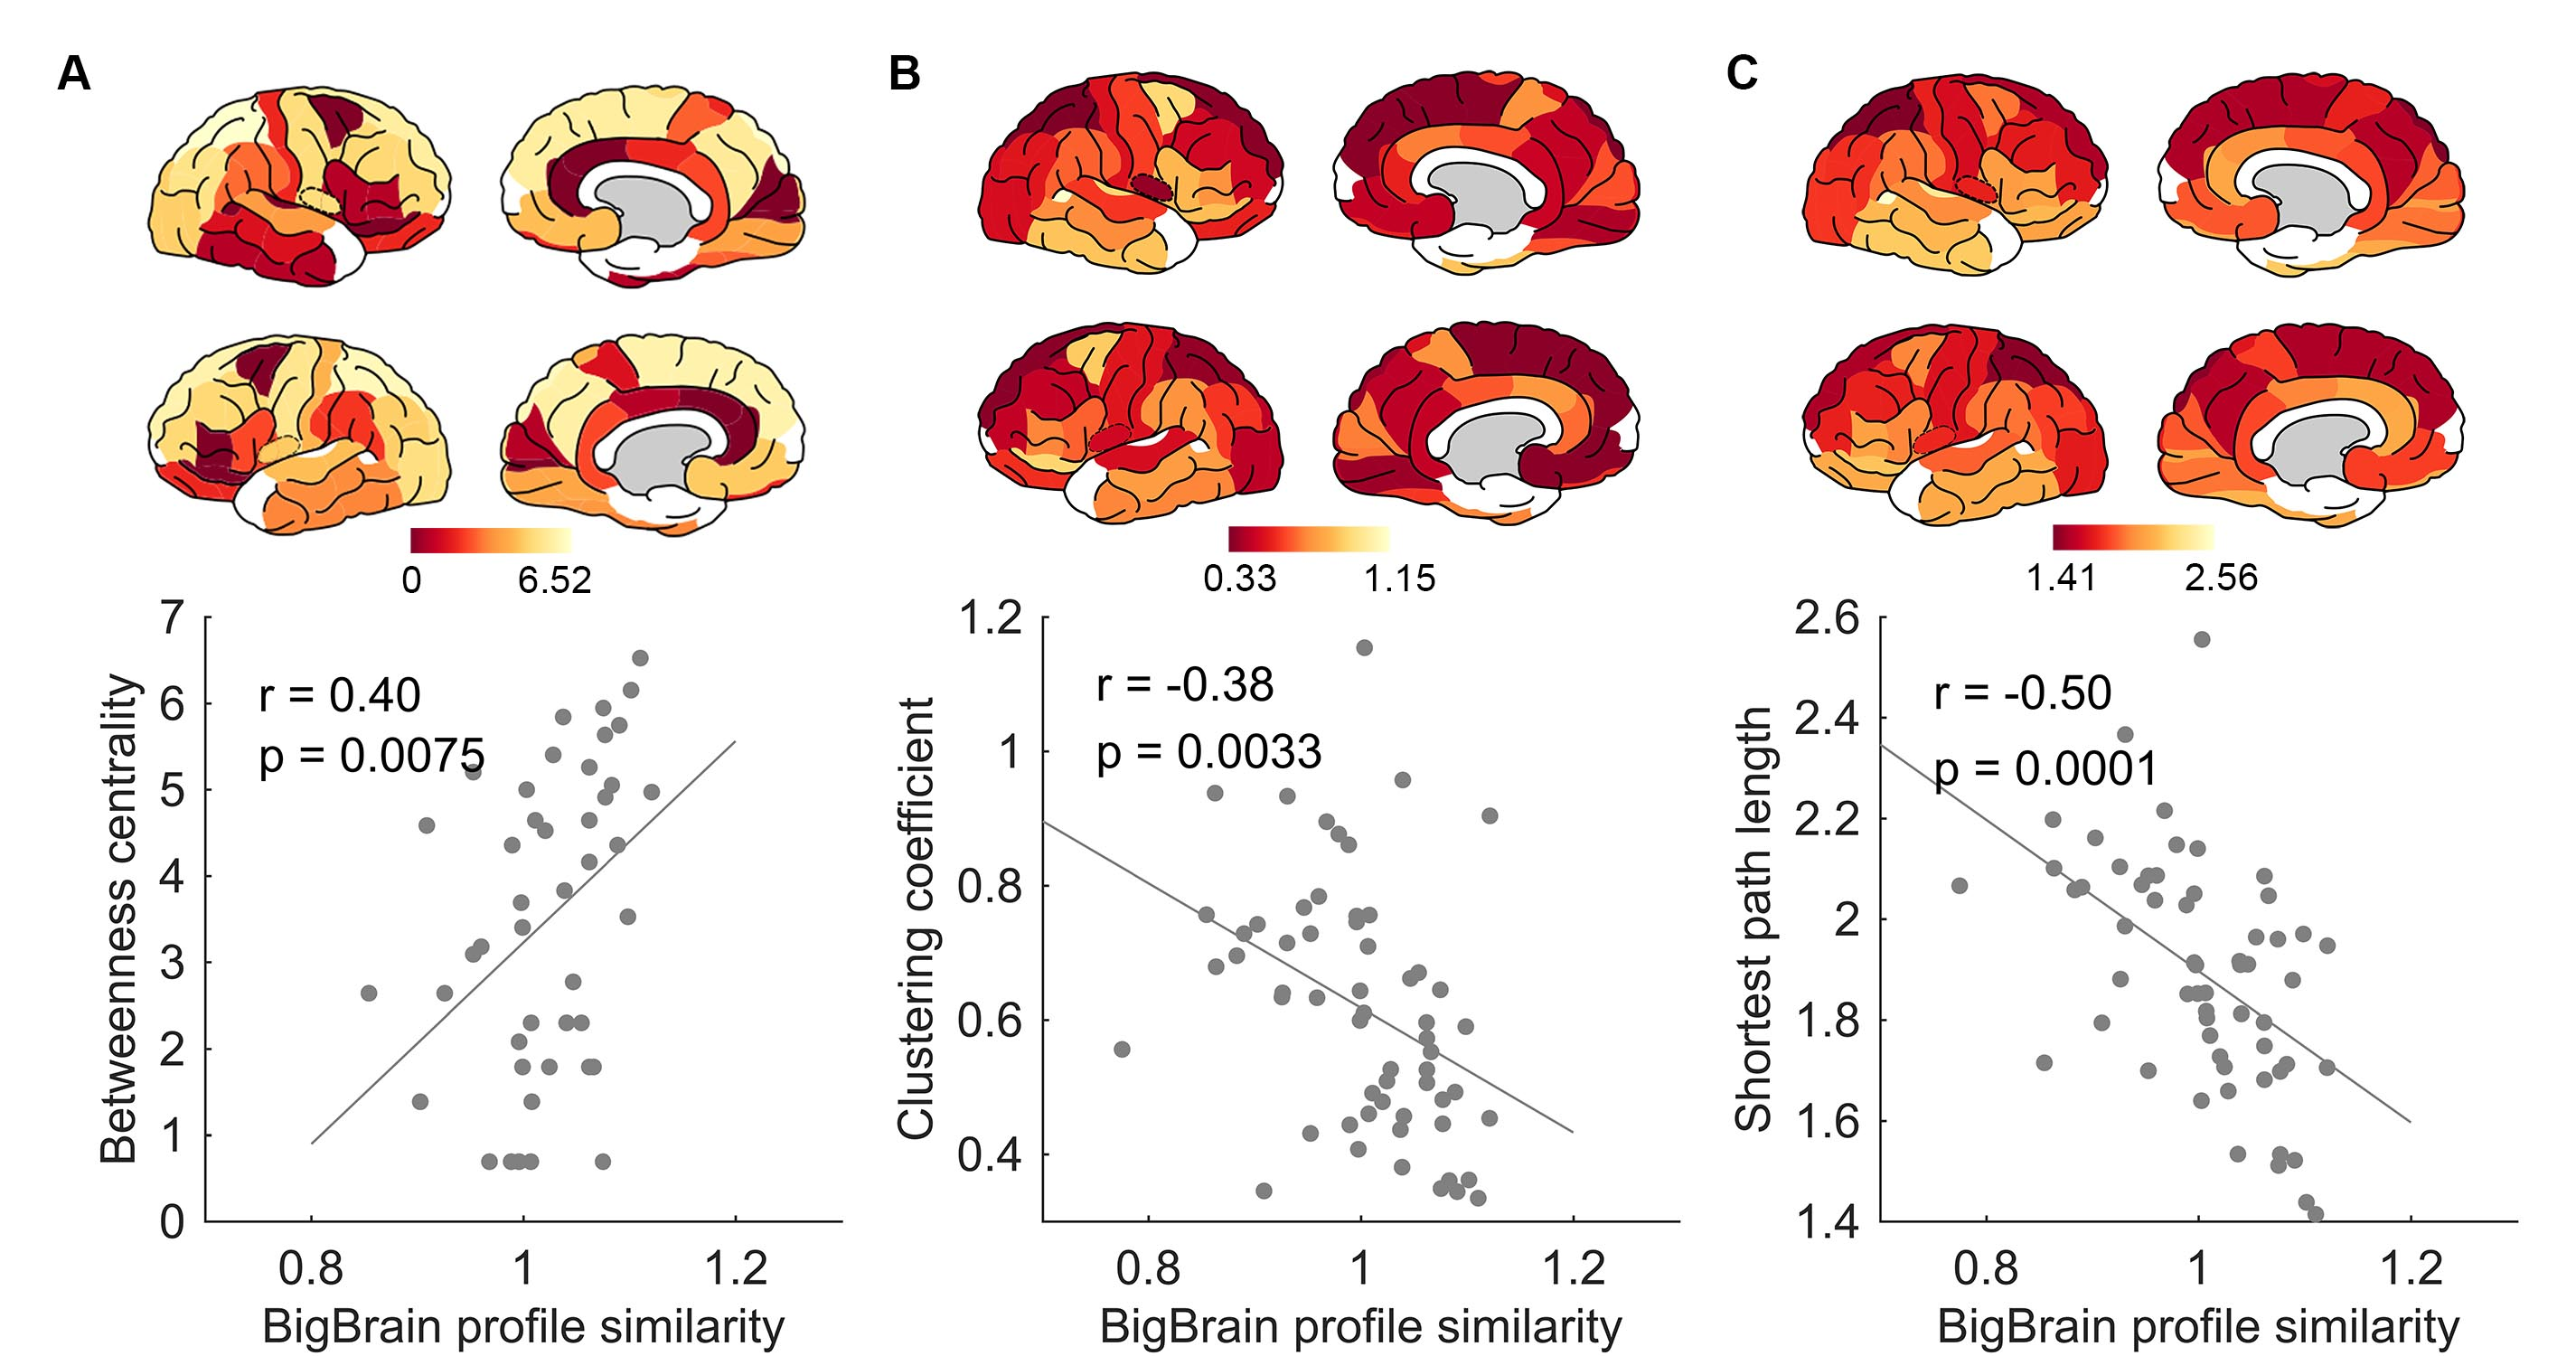
\includegraphics[width=\linewidth]{images/thesis_bb_fig6.jpg}
    \caption{The association of regional BigBrain profile similarity with (A) betweenness centrality (\rval = 0.40, \pval = 0.0075), (B) clustering coefficient (\rval = -0.38, \pval = 0.0033), and (C) mean shortest path length (\rval = -0.50, \pval = 0.0001) of the group-weighted network (NOS weights).}
    \label{bigbrainFig6}
\end{figure}


\section*{Discussion}
In this study, we investigated how cortical cytoarchitecture differentiation was associated with macroscale connectome organization. Data from the BigBrain project was used to extract laminar cytoarchitecture profiles across the entire cerebral cortex. BigBrain profile similarity for cortico-cortical connections was found to be significantly higher than for nonconnections, indicating that regions with higher similarity in laminar cytoarchitectonic patterns are more likely to be connected. Furthermore, the pattern of regional BigBrain profile similarity was strongly correlated with the pattern of nodal strength, clustering coefficient, and shortest path length of the structural network, suggesting that cortical regions with higher cytoarchitectonic similarity tend to be linked by stronger white matter connections and to be more involved in global integration. Taken together, our findings suggest that microscale cortical cytoarchitecture similarity is closely associated with macroscale brain connectome organization.\\

The use of cytoarchitecture profiles to quantify variation in human cerebral cortical architecture has a long history \citep{HAUG1956,MACKEY20091089,SCHLEICHER1986221,Schleicher2009,WREE198229}. In addition to classical histological methods, cytoarchitectonic profiles as provided by the BigBrain dataset allow for investigation of gradual changes in the volume fraction of cell bodies from pial surface to white matter surface, rather than concentrating on a particular cell type of a single layer \citep{Amunts2015ArchitectonicMO}. A rich body of literature examining the difference in profile shape between adjacent blocks within the cortical ribbon has provided strong evidence for the position of interareal borders \citep{Caspers2012CytoarchitectonicalAA,Schleicher2009,Schleicher1999ObserverIndependentMF,Schleicher2000ASA,Kujovic2012CytoarchitectonicMO}. Moreover, findings have also shown that vertically oriented cortical columns have similar laminar patterns of cell types and cell densities \citep{Zilles2010CentenaryOB}. Here, we used regional averaged BigBrain profiles to represent the intra-area laminar cytoarchitectonic pattern. Our validations revealed that the regional BigBrain profile features were associated with the areal characteristics of neuronal size and density proposed by von Economo and Koskinas (see Supporting Information, \citet{WEI2019bigbrain}), further indicating BigBrain profiles as a good representation of the microscale cytoarchitectonic features.\\

It has been eloquently reported that the presence of long-range cortico-cortical connection is associated with the cortical cytoarchitectonic patterning of the human and animal cortex. Cortical regions with more similar cytoarchitecture types have been suggested to have a larger chance to be connected, leading to the predictive structural model of cortico-cortical connections \citep{barbas2015general}. The structural model has been broadly verified in human prefrontal regions \citep{Barbas2005ParallelOO}, visual system of the cat \citep{Hilgetag2010CytoarchitecturalDA}, as well as the macaque \citep{beul2017predictive}, cat \citep{beul2015predictive}, mouse \citep{goulas2017principles}, and human cortex \citep{goulas2016cytoarchitectonic}. Further zooming in on neuronal morphology, macroscale highly connected cortical regions have been found to show a large pyramidal complexity in layer III, quantified among other things by a large basal dendritic tree size and a large number of spines per neuron in the macaque brain \citep{scholtens2014linking}, and a large neuronal soma size in the human brain \citep{van2015bridging}. Disruption in connectivity in brain disorders, such as schizophrenia, has also been observed to be associated to alterations in layer III pyramidal spine density \citep{VANDENHEUVEL2016293} and in vivo cortical cytoarchitectonic disruptions \citep{Wei2018CorticalMT}. Here, our findings demonstrate that strongly connected cortical regions show higher BigBrain profile similarity in the human brain cortex than regions with no connections. Compared with a prior study of the human brain that examined cytoarchitectonic similarity and connectivity \citep{goulas2016cytoarchitectonic}, the current study extends investigations by using the comprehensive BigBrain data with high spatial sampling rates and continuous descriptions of profiles from the pial to the white matter surface. Consistent findings across studies together support the structural model hypothesis of associated microscale cortical cytoarchitectonic organization and macroscale cortico-cortical connectivity in the mammalian brain \citep{barbas2015general,Barbas2005ParallelOO,beul2017predictive,beul2015predictive,goulas2016cytoarchitectonic,goulas2017principles,Hilgetag2010CytoarchitecturalDA}.\\

The neurobiological mechanism underlying the observed association between cytoarchitectonic similarity and cortico-cortical connectivity remains to be determined. A probable explanation has been provided in the context of brain ontogenesis, which argues that the development of cortical cytoarchitecture is associated with the establishment of connections \citep{barbas2015general,beul2017predictive,beul2015predictive,goulas2016cytoarchitectonic,goulas2017principles}. According to this hypothesis, the variation of laminar structure within the cerebral cortex arises during development, differentiating limbic areas with a relatively short developmental path combined with a poorly defined cortical layers from the longer developing association areas with well-delineated layer structures \citep{Barbas2016HowTP}. Cortical regions with similar laminar cytoarchi tecture patterns may thus develop during a similar time window \citep{barbas2015general,beul2017predictive,beul2015predictive,goulas2016cytoarchitectonic,goulas2017principles}. Furthermore, the formation of cortico-cortical connections has been argued to be shaped by the cortical cytoarchitecture development. Evidence has shown that connections originating from neurons in the early developed limbic cortices terminated in layer I of other areas \citep{barbas2015general}, known to be one of the earliest formed layers of the neocortex \citep{MarnPadilla1970PrenatalAE}. Together, the revealed association between cortical cytoarchitecture similarity and cortico-cortical connectivity may reflect the overlap in time windows of their development.\\

A number of remarks have to be made when interpreting the findings of our study. First, it is noted that regional difference in cortical volume could be of influence on the here reported association. We therefore performed additional analyses using streamline density as connection weight to correct for regional cortical volume, as well as a partial correlation analysis taking the number of BigBrain profiles per region as covariates (because larger regions will have more profiles). Both analyses showed results similar to the main analysis. Additionally, changing the region exclusion threshold to 0 or 50 BigBrain profiles revealed similar correlations, further suggesting that small regions with relative few profile samples had no specific effect on the results. Second, the BigBrain data was obtained from a single 65-year-old male donor. As a result, our analysis did not take into account possible individual variability, gender differences, and aging effects on profile similarity \citep{Shaw2008NeurodevelopmentalTO,Zilles1997QuantitativeAO}. Studies constructing a microscale reference brain based on a larger dataset would be of particular interest. Third, reconstruction of the macroscale connectome was limited by the current techniques of in vivo MRI. Diffusion imaging relies on water diffusion as an indirect probe of axon geometry, which has well-known limitations with respect to the reconstruction of complicated pathways \citep{Jbabdi2011TractographyWD}. High-field imaging, acquisition of more diffusion directions, and application of advanced white matter pathway reconstruction protocols may result in better detection of complicated fibers.\\

This study uses the state-of-the-art BigBrain dataset to obtain comprehensive cortical cytoarchitecture profiles of the human brain and shows an association of laminar profile similarity with anatomical network organization. Findings provide new evidence for a potential interplay between microscale cortical cytoarchitecture organization and macroscale cortico-cortical connectivity, which provide insights into the neurobiological mechanisms underlying the macroscale brain connectome. Understanding the cross-modal interaction between the micro- and macroscale of human brain organization may pave a new avenue for unraveling neuropathology in neurological and psychiatric disorders involving disruptions on both ends of the scale.

\section*{Acknowledgements}
We thank Marcel A. de Reus for his help with data processing. We appreciate Maurits Ridder for his contribution in collecting data. Diffusion weighted imaging data were kindly provided in part by the Human Connectome Project, WU-Minn Consortium (Principal Investigators: David van Essen and Kamil Ugurbil; 1U54MH091657) funded by the NIH Institutes and Centers that support the NIH Blueprint for Neuroscience Research; and by the McDonnell Center for Systems Neuroscience at Washington University.

\section*{Author Contributions}
Yongbin Wei: Investigation; Methodology; Writing – original draft; Writing – review \& editing. Lianne H. Scholtens: Writing – original draft; Writing – review \& editing. Elise Turk: Data curation; Writing – original draft; Writing – review \& editing. Martijn P. van den Heuvel: Conceptualization; Funding acquisition; Investigation; Project administration; Supervision; Writing – review \& editing.

\section*{Funding Information}
Martijn P. van den Heuvel, Nederlandse Organisatie voor Wetenschappelijk Onderzoek (http://dx.doi.org/10.13039/501100003246), Award ID: VIDI-452-16-015; Nederlandse Organisatie voor Wetenschappelijk Onderzoek, Award ID: ALWOP.179, and a Fellowship of MQ. Yongbin Wei, China Scholarship Council, Award ID: 201506040039.

\printbibliography[heading=subbibliography]

\end{refsection}

% SI
\begin{refsection}
\newpage
\section*{Supplementary Information}
\subsection*{Validations using alternative processing strategies}
Results were validated by adopting different processing strategies, including applying the 114-region subdivision DK atlas, setting the region inclusion threshold to 0 and 50 profiles, and generating the group average network at a threshold of 40\% and 60\% prevalence.

First, using the 114-region subdivision DK atlas, the BigBrain profile similarity between inter-connected cortical regions was found to be consistently higher than between non-connected regions (\tval = 12.5, \pval = 3 $\times$ 10\textsuperscript{-35}). The pattern of regional BigBrain profile similarity was also reliably correlated with both the pattern of nodal strength of the group weighted network (NOS: \rval = 0.38, \pval = 0.0001) and nodal degree of the group binary network (\rval = 0.35, \pval = 0.0004). These findings suggested that our main results were not driven by the selection of cortical parcellations. 

Second, setting the region inclusion threshold to 0 (meaning that all regions were included) and 50 profiles (meaning that only regions with more than 50 profiles were included), BigBrain profile similarity for connections was significantly higher than for non-connections (\tval = 12.2, \pval = 3 $\times$ 10\textsuperscript{-33} for regions with >0 profile, \tval = 8.9, \pval = 3 $\times$ 10\textsuperscript{-18} for regions with >50 profiles). Significant correlations were also found between the pattern of regional BigBrain profile similarity and nodal strength (\rval = 0.55, \pval < 0.0001 for regions with >0 profile, \rval = 0.54, \pval = 0.0001 for regions with >50 profiles) and degree (\rval = 0.52, \pval < 0.0001 for regions with >0 profile, \rval = 0.48, \pval = 0.0008 for regions with >50 profiles), indicating the exclusion of small regions did not change the nature of our results. 

Third, thresholding the group structural network at 40\% or 60\% revealed similar findings: a significantly higher BigBrain profile similarity was found for connections as compared to non-connections (40\%: \tval = 10.6, \pval = 1 $\times$ 10\textsuperscript{-25}, 60\%: \tval = 10.2, \pval = 6 $\times$ 10\textsuperscript{-24}), and a significant correlation was found between the pattern of BigBrain profile similarity and nodal strength (40\%: \rval = 0.56, \pval < 0.0001, 60\%: \rval = 0.55, \pval < 0.0001) and degree (40\%: \rval = 0.52, \pval < 0.0001, 60\%:  \rval = 0.51, \pval < 0.0001). These results indicated that different structural network density did not alter our main results.

\subsection*{Validations using the raw correlation coefficients}
The raw correlation coefficient between BigBrain profiles was taken as the measurement of similarity to examine the influence of the performed normal-distribution transformation. We consistently found significant differences of BigBrain profile similarity between interconnected cortical regions and non-connected regions (\tvaldf(1,709) = 7.64, \pval < 0.0001), as well as the significant correlation of profile similarity with connection strength (NOS: \rval = 0.22, \pval < 0.0001). Moreover, the pattern of regional BigBrain profile similarity was also associated with the nodal degree (\rval = 0.41, \pval = 0.0013) and strength (\rval = 0.45, \pval = 0.0003, NOS weighted), confirming that our main results were not affected by the normal-distribution transform.

\subsection*{Validating BigBrain profiles using von Economo-Koskinas data}
We assessed the agreement of BigBrain profiles with the cytoarchitectonic data derived from von Economo and Koskinas (EK) atlas \citep{von1925cytoarchitektonik}. BigBrain profiles were registered to the FreeSurfer-based EK atlas \citep{Scholtens2015ECONOMO} and averaged within each EK region. In parallel, information of laminar layer thickness, neuron cell size, and neuron density of each area were taken from the EK atlas to generate EK profiles describing the level of [cell size $\times$ density] from pial surface to white matter surface. EK profiles were additionally resampled to 1000 discrete steps to match the BigBrain profiles (Fig. S2). We correlated BigBrain profiles with the EK profiles for each EK region and observed significant associations between the two types of profiles (\rval = 0.52 $\pm$ 0.17, ranging from 0.24 to 0.83 for all EK areas), indicating the BigBrain profiles to be comparable with the laminar cytoarchitecture in classic EK atlas.

Furthermore, cortical thickness estimates derived from BigBrain profiles were also found to be significantly correlated to Von Economo-Koskinas’s measures of thickness across cortical regions (\rval = 0.61, \pval = 0.0005, FDR corrected) (Fig. S2), indicating that the co-registration process of BigBrain profiles in the current study yielded output which provided consistent measurement of cortical morphology. The regional averaged mean and SD of BigBrain profiles showed significant correlations with the regional mean and SD of EK profiles across all cortical regions (\rval = 0.51, \pval = 0.0082 and \rval = 0.57, \pval = 0.0024, for the mean and SD, respectively, FDR corrected) (Fig. S3), suggestive of the consistency in cortical cytoarchitectonic patterns.

\subsection*{Examining effects of DK area size}
In order to examine the effects of DK area size on our results, we first obtained the mean cortical volume and surface area for each DK region, by averaging across all subjects in the HCP dataset. The cortical volume and surface area were observed to be correlated with the regional BigBrain profile similarity (volume: \rval = 0.50; surface area: \rval = 0.53; both \pval < 0.0001) and connectivity degree (volume: \rval = 0.69; surface area: \rval = 0.74; both \pval < 0.0001)/strength (volume: \rval = 0.75; surface area: \rval = 0.80; both \pval < 0.0001). Next, we regressed out the cortical volume and surface area, separately, from both the regional BigBrain profile similarity and nodal degree/strength using the linear regression. Residuals after the regression were used to re-perform the correlation. We observed a decreased effect of correlations between regional profile similarity and nodal degree/strength, but the significance still held mostly (volume: \rval = 0.29, \pval = 0.0165, for degree; \rval = 0.31, \pval = 0.0106, for strength; surface area: \rval = 0.23, \pval = 0.0592, for degree; \rval = 0.25, \pval = 0.0423, for strength). These findings suggested that the association of BigBrain profile similarity pattern with nodal degree/strength was not entirely driven by the DK area size.

\subsection*{Within-region profile heterogeneity}
In the current study, distinct numbers of BigBrain profiles were extracted from cortical regions and averaged within the same region, resulting in the consideration of potential effects of within-region profile heterogeneity and “smoothness” caused by averaging profiles. We thus performed three additional analyses to examine whether these effects played a role in our main findings.

First, we calculated the Kendall's coefficient of concordance (KCC) for profiles of each cortical region to represent the within-region profile homogeneity. KCC was computed as follows:
\[
W = \frac{\sum (R_{i})^{2} - N\overline{R}}{\frac{1}{12} K^{2}(N^{3} - N)} \]
where \textit{W} is the KCC within each cortical region, ranged from 0 to 1; \textit{R}\textsubscript{i} the sum rank of the \textit{i}\textsubscript{th} depth level; $\mathsf{\overline{R}}$ the mean of \textit{R}\textsubscript{i}; \textit{K} the number of profiles within a cortical region; and N the number of ranks (i.e., depth levels; here, \textit{N} = 1000). The resultant regional KCC ranged from 0.22 to 0.67 with mean $\pm$ SD of 0.51 $\pm$ 0.09 (Fig. S4A). The pattern of KCC did not correlate with the pattern of BigBrain profile similarity across the cortex (\rval = -0.07, \pval = 0.55), nor with the pattern of regional connectivity strength (\rval = 0.06, \pval = 0.63) (Fig. S4B), suggesting that variations of within-region profile heterogeneity did not drive the observed association between BigBrain profile similarity and cortico-cortical connectivity.

Second, we performed a permutation test to examine whether within-region profile homogeneity is higher than the homogeneity of randomly selected profiles. We randomly shuffled the DK region label for all profiles and computed KCC within the randomly assigned regions. The average KCC of all regions was recorded. The computation was permutated 10,000 times to generate a null distribution of KCC. Comparing the original averaged KCC (i.e., 0.51) to the null distribution revealed a significance level of \pval < 0.0001 (Fig. S4C), indicating that within-region profile heterogeneity is significantly higher than within randomly selected profiles.

Third, we randomly chose 20 BigBrain profiles from profiles of each cortical region and averaged these profiles to obtain a region-wise BigBrain profile. Selecting 50 profiles showed similar results (data not shown). In this manner, the same number of BigBrain profiles was included to generate the regional profile, ruling out the potential effect of different sizes of profile samples. We repeated the randomization 10,000 times and consistently found a higher BigBrain similarity between connected regions than non-connected regions (T ranged from 7.18 ~ 12.16, mean $\pm$ SD = 9.88 $\pm$ 0.55, all \pval < 0.0001) (Fig. S4D). Furthermore, the pattern of regional BigBrain profile similarity reliably showed correlations with the pattern of connectivity degree (\rval ranged from 0.17 - 0.57, mean $\pm$ SD = 0.38 $\pm$ 0.05, more than 99.1\% randomizations showed \pval < 0.05) and strength (\rval ranged from 0.21 – 0.61, mean $\pm$ SD = 0.42 $\pm$ 0.05, more than 99.9\% randomizations showed \pval < 0.05) (Fig. S4E), suggesting that these findings were not affected by the distinct “smoothness” levels derived from different profile sample sizes.

\subsection*{Supplementary References}
\printbibliography[heading=none]

\end{refsection}



\pagestyle{MyStyle}

\chapter{Genetic mapping and evolutionary analysis of human-expanded cognitive networks}
\label{ch:HAR}


\begin{flushright}
\textit{Yongbin Wei, Siemon C. de Lange, Lianne H. Scholtens, Kyoko Watanabe, Dirk Jan Ardesch, Philip R. Jansen, Jeanne E. Savage, Longchuan Li, Todd M. Preuss, James K. Rilling, Danielle Posthuma, Martijn P. van den Heuvel}\\
Nature Communications, 2019; 10: 4839
\vspace{7 mm}

\end{flushright}

\begin{refsection}
\newpage
\section*{Abstract}
Cognitive brain networks such as the default-mode network (DMN), frontoparietal network, and salience network, are key functional networks of the human brain. Here we show that the rapid evolutionary cortical expansion of cognitive networks in the human brain, and most pronounced the DMN, runs parallel with high expression of human-accelerated genes (HAR genes). Using comparative transcriptomics analysis, we present that HAR genes are differentially more expressed in higher-order cognitive networks in humans compared to chimpanzees and macaques and that genes with high expression in the DMN are involved in synapse and dendrite formation. Moreover, HAR and DMN genes show significant associations with individual variations in DMN functional activity, intelligence, sociability, and mental conditions such as schizophrenia and autism. Our results suggest that the expansion of higher-order functional networks subserving increasing cognitive properties has been an important locus of genetic changes in recent human brain evolution.

\section*{Introduction}
The human brain is capable of supporting a wide range of complex cognitive abilities, more so than other highly developed and intelligent great apes, such as the chimpanzee, one of our closest living evolutionary relatives with which we share the majority of our genetic material \citep{britten2002divergence}. This distinction in cognitive abilities is commonly believed to be associated with the rapid expansion of multimodal association areas and their structural and functional connections in the human brain \citep{buckner2013evolution,preuss2017chapter,ardesch2019evolutionary}, with cognitive functional networks, such as the frontoparietal network, salience network, and default-mode network (DMN), playing an essential role in higher-order brain functions \citep{buckner2008brain,raichle2015brain,uddin2015salience}. These cognitive functional networks are highly heritable \citep{glahn2010genetic,ge2017heritability} and relate to genetic effects associated with neuron growth and metabolism \citep{wang2015correspondence}. Uncovering the evolutionary genetic underpinnings of cognitive functional networks, and in particular, to what extent cognitive functional networks have developed in recent human evolution, is crucial for our understanding of the high cognitive complexity of human brain function.

The DMN in particular has been identified as a central network in human cognition, consisting of densely connected areas such as the posterior cingulate, precuneus, inferior parietal, middle temporal, and medial prefrontal cortices \citep{buckner2008brain,raichle2015brain}. Comparative neuroimaging studies have shown default-mode activity in chimpanzees \citep{barks2013default} and macaques \citep{mantini2011default}, but with potential subtle differences in both the spatial and topological layout of this central network \citep{miranda2014bridging}-changes that may relate to enhancement of cognitive functions in humans compared to other primate species. The DMN is central to social cognition, including aspects of mental self-projection \citep{buckner2007self}, mental rehearsal of future actions \citep{tulving2005episodic}, and understanding of another person’s mental perspective. These advanced social abilities are likely to have been highly adaptive during recent human evolution \citep{tomasello2010ape}, potentially enabling humans to make more complex social inferences \citep{buckner2007self}.

Here, we studied the expansion and evolutionary genetics of higher-order cognitive networks in recent human brain evolution, with a particular focus on the evolutionarily genetic drive of the DMN. Recent genome-wide studies comparing the human genome with that of the chimpanzee have identified a unique set of loci that displayed accelerated divergence in the human lineage \citep{pollard2006rna,pollard2006forces}. Genes associated with these so-called human accelerated regions (HAR) have been linked to neuron development, but also the development of brain disorders such as autism spectrum disorder (ASD) \citep{doan2016mutations}. We integrate genetic data with comparative neuroimaging and present that regions of higher-order cognitive networks are highly expanded in recent human brain evolution. We show that HAR genes likely have played a crucial role in this, being highly expressed in expanded cognitive networks (and in particular the DMN) and being differentially expressed in the human brain compared to chimpanzees and macaques. We provide further evidence of HAR and DMN genes to be important in human cognitive functioning, social behavior, and mental disorders, such as autism and schizophrenia.

\begin{figure}[h]
    \centering
    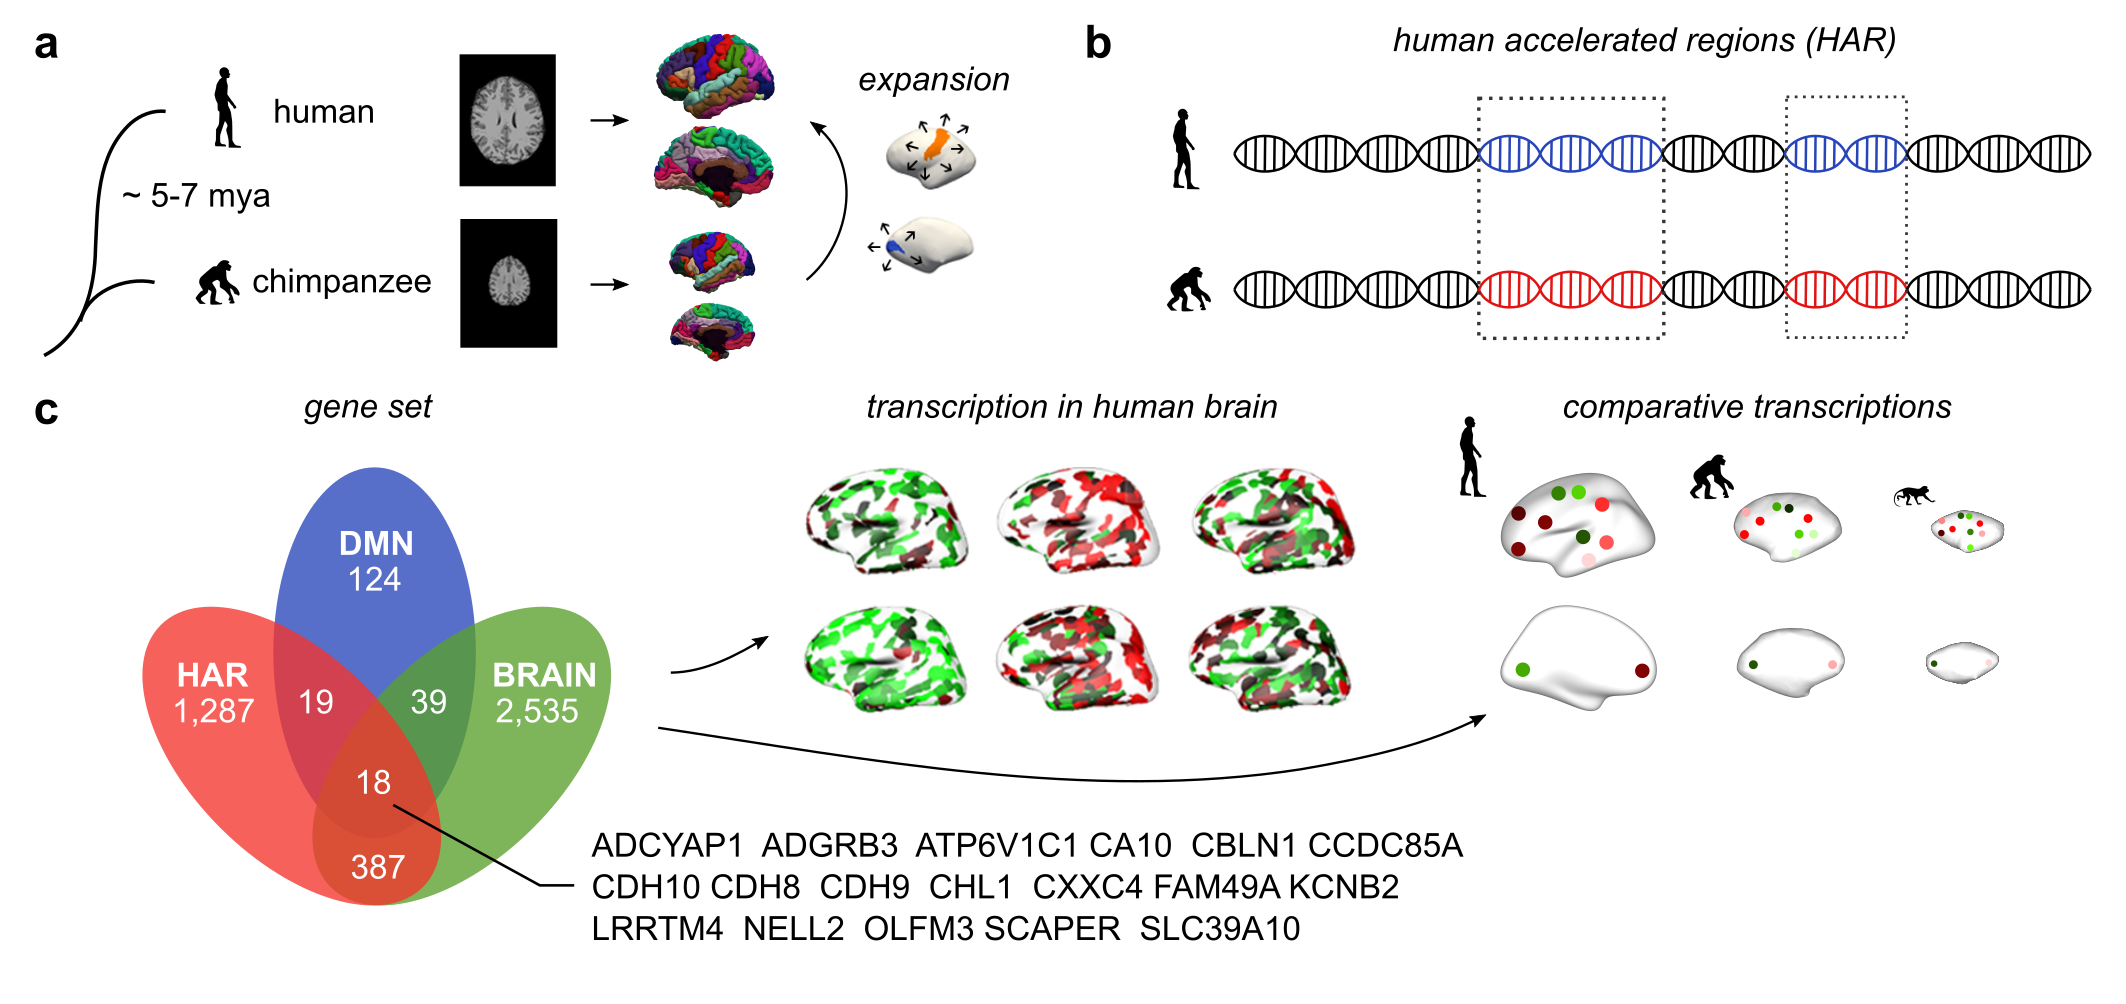
\includegraphics[width=\linewidth]{images/harFig1.png}
    \caption{Methods overview. a The human and chimpanzee cortex were constructed using MRI data, with chimpanzee-to-human cortical expansion computed based on the reconstructed cortical maps. b Genes associated with human accelerated regions (HAR), which represent genomic loci with accelerated divergence in humans, were examined. c Cortical gene expression of HAR genes and HAR-BRAIN genes were examined using human transcription data from the Allen Human Brain Atlas (AHBA) and comparative transcription data of the human, chimpanzee, and macaque from the PsychENCODE database}
    \label{harFig1}
\end{figure}

\section*{Results}
\subsection*{Human cortical expansion}
We started by mapping the expansion of the human cortex (\textit{Homo sapiens}) compared to the cortex of the chimpanzee (\textit{Pan troglodytes}), one of our closest living evolutionary relatives along with the bonobo (\textit{Pan paniscus}). Cortical morphometry of the chimpanzee and human cortex was assessed using a surface-to-surface mapping of 3D reconstructions of the cortical mantle across both species, based on in vivo T1-weighted MRI (29 chimpanzees, 30 humans; Fig. 1a). The largest expansion of the human cortex was found in areas of bilateral orbital inferior frontal gyrus ($\times$4.0 expansion), rostral middle frontal lobe ($\times$3.8 expansion), inferior/middle temporal lobe ($\times$3.0/2.9 expansion), lingual gyrus ($\times$2.9 expansion), right inferior parietal lobe ($\times$3.7 expansion), and left precuneus ($\times$2.7 expansion; two-sample t-test on the normalized expansion, \textit{q} < 0.001, false discovery rate [FDR] corrected; Cohens'\textit{d} > 0.989; Fig. 2a). The lowest expansion was found in primary areas, including bilateral precentral gyrus ($\times$1.3 expansion), postcentral gyrus ($\times$1.4 expansion), and paracentral lobe ($\times$1.2 expansion; \textit{q} < 0.001, FDR corrected; Cohens'\textit{d} < -1.047; Fig. 2a and Supplementary Data 1).

We next grouped cortical areas into the visual (VN), somatomotor (SMN), dorsal-attention (DAN), limbic (LN), ventral-attention (VAN, also commonly referred to as the salience network), frontoparietal (FPN), and default-mode network (DMN) (Fig. 2b and Supplementary Methods)\citep{thomas2011organization}. Higher-order cognitive networks (i.e., DMN, FPN, VAN) displayed particularly high levels of cortical expansion as compared to the SMN/VN ($\times$1.2 larger expansion in regions of higher-order cognitive networks combined compared to the regions of the SMN/VN combined, two-sample t-test, \tvaldf(86) = 3.257, \pval = 0.002; Fig. 2d). FPN showed the largest expansion (mean: $\times$2.9 expansion), with the DMN in second place (mean: $\times$2.4 expansion), showing both significantly higher expansion when comparing each of them with the rest of the brain (FPN: \tvaldf(108) = 3.360, \pval = 0.001; DMN: \tvaldf(108) = 2.621, \pval = 0.010; FDR corrected; Supplementary Table 1). In contrast, separately examining the other five networks did not show significant increases in the expansion of these networks compared to the rest of the cortex.

\begin{figure}[h]
    \centering
    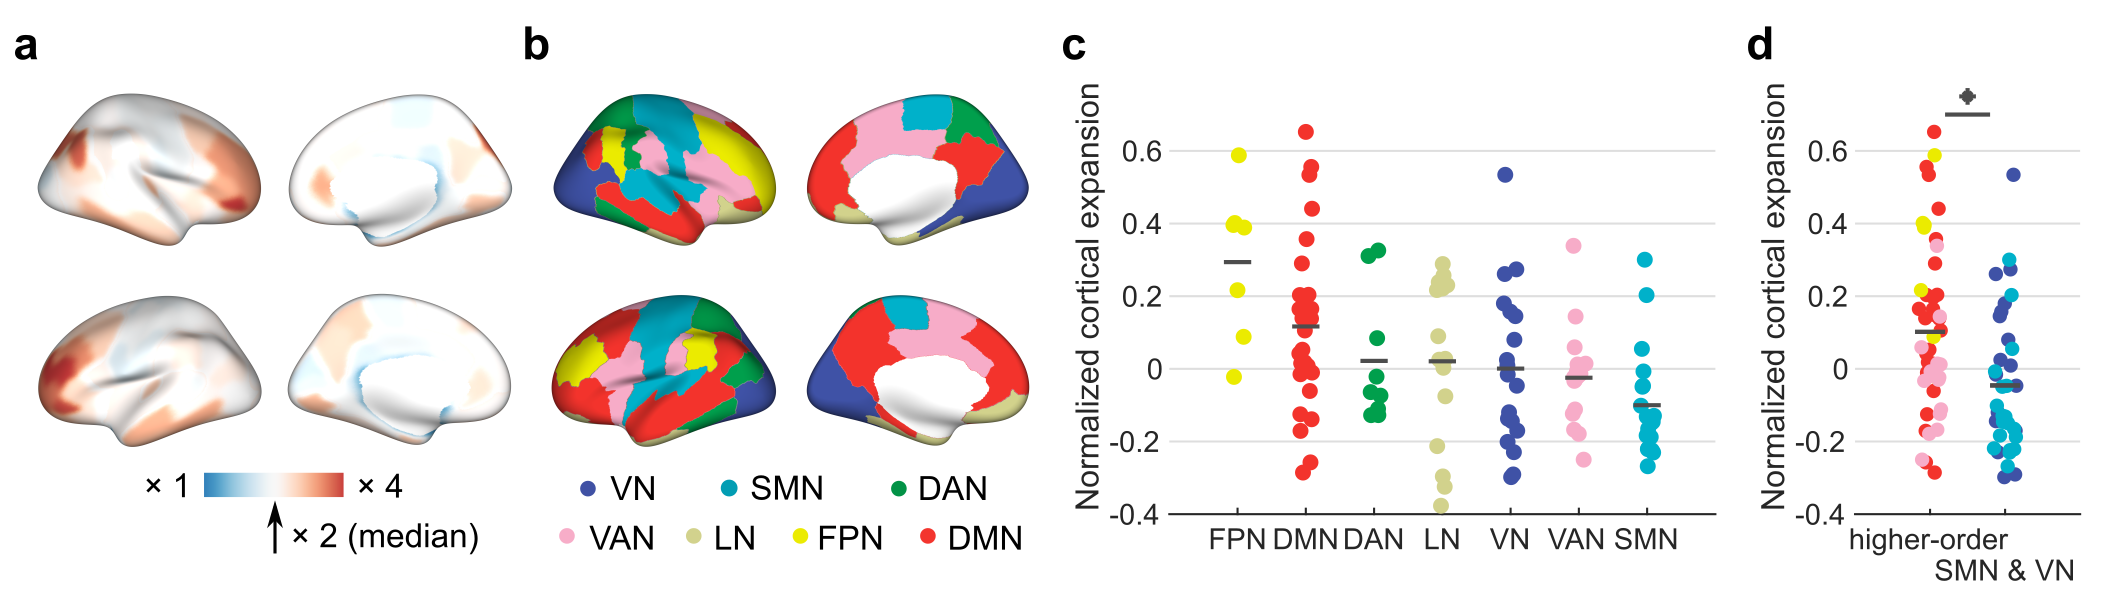
\includegraphics[width=\linewidth]{images/harFig2.png}
    \caption{Cortical expansion. a Cortical expansion from chimpanzees to humans. Blue: below-median human expansion (i.e., < $\times$2 expansion compared to chimpanzee); red: above-median expansion (i.e., > $\times$2). b Brain maps of the seven resting-state functional networks according to the DK-114 atlas, describing the visual (VN), somatomotor (SMN), dorsal-attention (DAN), limbic (LN), ventral-attention (VAN), frontal-parietal (FPN), and default-mode network (DMN). c Levels of normalized cortical expansion per functional network in descending order of mean expansion. d Levels of normalized cortical expansion in higher-order cognitive networks (DMN, FPN, VAN) versus the SMN and VN. Dots depict cortical regions. Colors represent functional networks, as in panel b. Central marks are mean expansions. \* indicates a two-sided p-value < 0.05, FDR corrected, two-sample t-test. Source data provided as Source Data file}
    \label{harFig2}
\end{figure}

\subsection*{HAR gene expression}
We then examined this distinct pattern of human cortical expansion across the seven resting-state functional networks in relation to cortical gene expression patterns relevant to human evolution. Microarray data on gene expression across cortical regions were obtained from the Allen Human Brain Atlas (AHBA) (http://human.brain-map.org/), containing transcriptional profiles of 20,734 genes across 57 areas of the left cortical mantle (Fig. 1c). Genes relevant to human evolution were taken as the list of 2143 genes associated with HAR as presented previously by Doan and colleagues \citep{doan2016mutations}, selected based on positional mapping. Alternative selection and allocation of HAR-associated genes are possible (e.g., using chromatin interactions) and we examined such alternatives to validate our results (Supplementary Note 1).

Transcription data of 1711 HAR-associated genes were present in AHBA (referred to as HAR genes; Supplementary Data 2), and we further examined their cortical gene expression levels in comparison to the cortical expansion. The expression profile of HAR genes was positively correlated to the pattern of human cortical expansion (Pearson's \rvaldf(53) = 0.360, \pval = 0.007; Supplementary Fig. 1a), indicating the highest HAR gene expression in highly expanded areas of the human cortex. This association significantly exceeded the null condition of correlations between cortical expansion and expression of random gene sets (i.e., 1711 random genes) selected from a pool of 8686 genes related to general evolutionarily conserved genetic elements (ECE genes \citep{lindblad2011high}; \pval < 0.001, permutation test, 10,000 permutations; Supplementary Fig. 1a). Cortical regions of cognitive networks also showed significantly higher expression of HAR genes compared to regions of the SMN/VN (\tvaldf(44) = 2.742, \pval = 0.009; FDR corrected; Supplementary Fig. 1b), with regions of the DMN showing the highest HAR gene expression (\tvaldf(55) = 2.274, \pval = 0.027, uncorrected, comparing the DMN to all other networks combined; Supplementary Fig. 1c). These effects again significantly exceeded the null conditions of effects of random ECE genes (all \pval < 0.001, 10,000 permutations). Furthermore, examining the other six functional networks separately did not show a significant enhancement of HAR gene expression (Supplementary Table 2).

\subsection*{HAR-BRAIN gene expression}
With the set of HAR genes describing genes involved in all sorts of functions across the entire human body (and thus not specific to 'brain'), we continued by examining whether HAR genes related to brain processes may have played a specific role in the large cortical expansion of cognitive functional networks in human evolution. We identified genes commonly expressed in brain areas using the GTEx database (https://www.gtexportal.org/), selecting 2979 genes significantly more expressed in brain tissues compared to other available body sites (\textit{q} < 0.05, FDR corrected; one-sided two-sample t-test; referred to as BRAIN genes); 415 genes (24.3\%) out of the full set of 1711 HAR genes were observed to be significantly more expressed in brain tissues, a set from now on referred to as HAR-BRAIN genes (in contrast to HAR-nonBRAIN genes; Supplementary Data 2).

We then aimed to examine (1) whether HAR-BRAIN genes were more expressed particularly in regions of higher-order cognitive networks compared to the total set of HAR genes, and (2) to what extent HAR-BRAIN genes were more expressed in regions of higher-order cognitive networks, more than an average set of genes related to general brain processes (i.e., BRAIN genes). First, the cortical expression pattern of HAR-BRAIN genes was significantly correlated with the pattern of human cortical expansion (\rvaldf(53) = 0.488, \pval < 0.001; Fig. 3c). Furthermore, HAR-BRAIN genes showed significantly higher expression in regions of cognitive networks as compared to the SMN/VN (\tvaldf(44) = 5.136, \pval < 0.001, FDR corrected; Fig. 3e), with the highest expression levels again observed in the DMN (\tvaldf(55) = 3.267, \pval = 0.002, FDR corrected, DMN versus the rest of the cortex; Fig. 3f). These effects were, respectively, $\times$3.2 and $\times$2.7 larger than the effect obtained by HAR-nonBRAIN genes (\tval(55) = 1.028, \pval = 0.309 and \tvaldf(55) = 1.212, \pval = 0.232, separately, Supplementary Fig. 2). Notably, examining the other six functional networks separately did not show any significant elevations of HAR-BRAIN gene expression (Supplementary Table 3), suggesting the highest expression level in the DMN.

\begin{figure}[h]
    \centering
    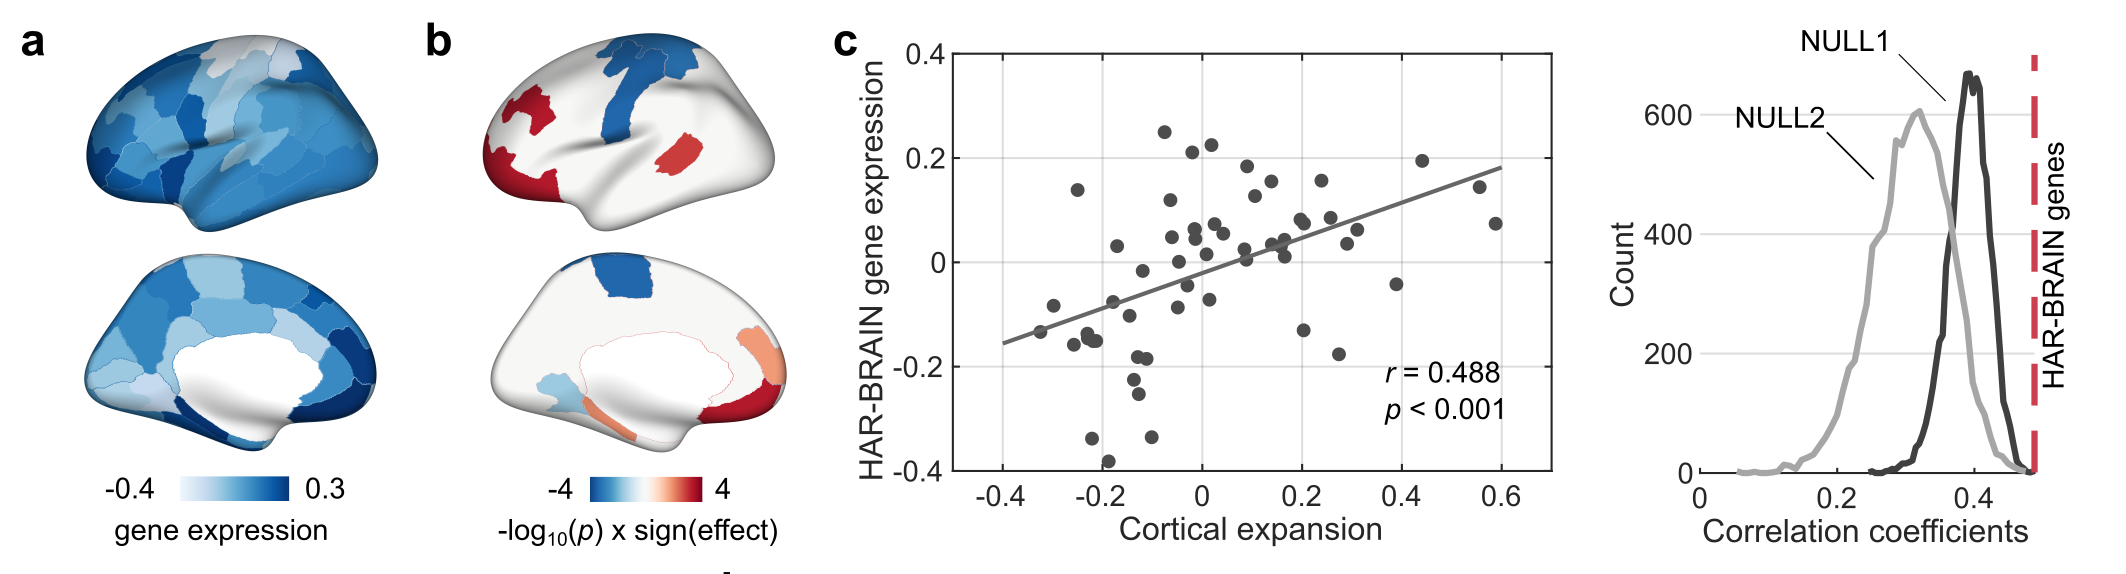
\includegraphics[width=\linewidth]{images/harFig3.png}
    \caption{HAR-BRAIN gene expression. a Cortical gene expression of HAR-BRAIN genes. b Cortical maps of the significance level obtained by permutation tests, comparing expressions of HAR-BRAIN genes to equally sized random gene-sets taken from BRAIN (NULL1) and ECE genes (NULL2). c Association between the gene expression profile of HAR-BRAIN genes and normalized cortical expansion between human and chimpanzee (left). The correlation coefficient is significantly higher than NULL1 and NULL2 (both p < 0.001, two-sided, permutation test; right).}
    \label{harFig3}
\end{figure}

Second, we compared HAR-BRAIN gene expression with two types of null-distributions of expression differences generated by randomly selecting the same number of genes (i.e., 415) from the pool of 2979 BRAIN genes (referred to as NULL1) and 8686 ECE genes (referred to as NULL2). The elevated expression of HAR-BRAIN genes in regions of higher-order cognitive networks was significantly larger than both null distributions (\pval = 0.006 and \pval < 0.001 for NULL1 and NULL2, respectively; 10,000 permutations; Fig. 3e). The same result was observed when examining DMN regions specifically (\pval < 0.001 for both NULL1 and NULL2; 10,000 permutations; Fig. 3f), suggesting a specific role of HAR-BRAIN genes in differentiating DMN regions from the rest of the brain. Permutation testing based on randomly shuffling cortical areas showed similar results (Supplementary Fig. 3). An exploratory examination on gene expression in each individual further demonstrated that the differentiation of HAR-BRAIN gene expression between the DMN and the rest of the cortex significantly correlated with the ratio of brain volume of the DMN regions (\rvaldf(4) = 0.839, \pval = 0.037; Supplementary Fig. 4).

\begin{figure}[h]
    \centering
    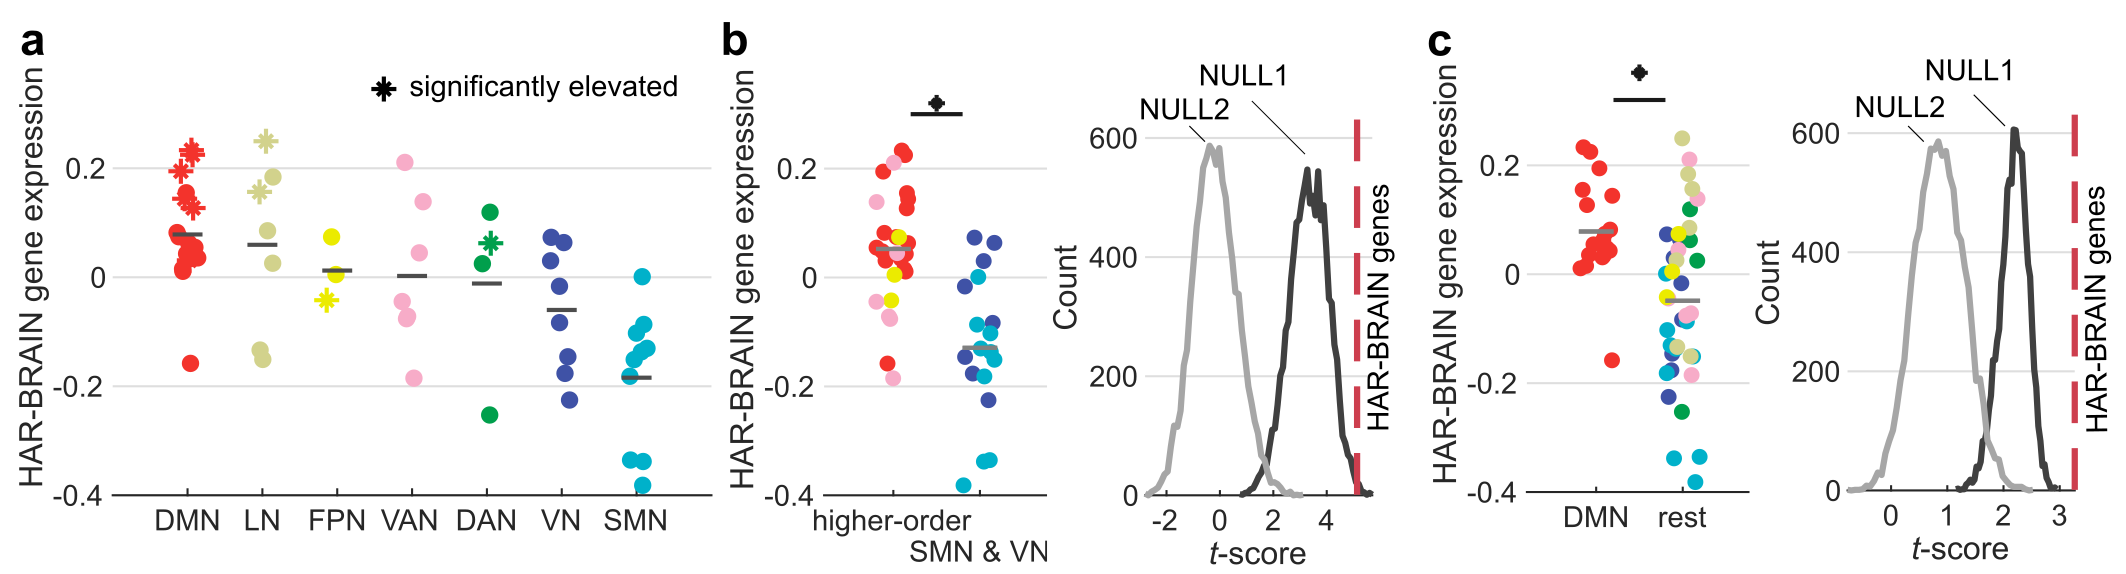
\includegraphics[width=\linewidth]{images/harFig4.png}
    \caption{d HAR-BRAIN gene expression within each of the seven functional networks ranked in descending order of the mean expression. Asterisks (*) indicates significantly upregulated regions as in panel b. e HAR-BRAIN gene expression in cognitive networks (DMN, FPN, and VAN) versus the SMN and VN (left), with permutation results demonstrated in the right panel (two-sided p = 0.003 and p < 0.001 for NULL1 and NULL2, respectively). f HAR-BRAIN gene expression in the DMN versus the rest of the cortex (left), with permutation results demonstrated in the right panel (two-sided p < 0.001 for both NULL1 and NULL2).}
    \label{harFig4}
\end{figure}

We then examined HAR-BRAIN expression for each of the cortical regions of the 7 functional networks separately; 10 cortical areas showed significantly high expression of HAR-BRAIN genes compared to a random selection of genes out of both BRAIN (NULL1) and ECE genes (NULL2) (FDR corrected, \textit{q} < 0.05; 10,000 permutations; Fig. 3b). Importantly, 7 out of these 10 regions described regions of the higher cognitive networks and 6 out of these 7 regions described DMN regions (\pval = 0.034 and 0.008, respectively; hypergeometric test). These findings together suggest a specific role of HAR-BRAIN genes in the architecture of cognitive functional brain networks, beyond effects of general evolutionary conserved genes and general BRAIN genes.

\subsection*{Chimpanzee-human comparative gene expression}
Our analyses so far suggested that HAR-BRAIN genes were more expressed in highly expanded regions of higher-order cognitive networks, but did not yet provide direct information on whether HAR-BRAIN gene expression is upregulated in the human brain compared to that of other primate species. To examine this, we used gene expression data from the PsychENCODE database (http://evolution.psychencode.org/) \citep{sousa2017molecular}, which describes gene expression of 11 comparable cortical regions across the human, chimpanzee, and macaque. Due to the lower spatial sampling of cortical regions (data of 3 DMN regions available, Fig. 3g), we limited our examination to a comparison between cognitive networks and the SMN/VN. First, we replicated the observation of high expression of HAR-BRAIN genes in regions of higher-order cognitive networks compared to regions of the SMN/VN in humans (\tvaldf(8) = 7.135, \pval < 0.001; Fig. 3h), with this effect significantly exceeding both NULL1 and NULL2 (both \pval < 0.001, 10,000 permutations). This confirmed our AHBA-based findings of high HAR-BRAIN gene expression in cognitive networks in the human brain. Second, the differentiating level of HAR-BRAIN gene expression between cognitive and primary areas observed in humans (Cohen's \textit{d} = 4.605) was found to be $\times$2.7 larger than the effects found in chimpanzees (Cohen's \textit{d} = 1.695) and $\times$2.8 larger compared to macaques (Cohen's \textit{d} = 1.616). Chimpanzees and macaques showed only marginally higher HAR-BRAIN gene expression in regions of higher-order cognitive networks as compared to the SMN/VN (chimpanzees: \tvaldf(8) = 2.626, \pval = 0.030; macaques: \tvaldf(8) = 2.504, \pval = 0.037). Furthermore, the difference in effect size between humans and chimpanzees was larger than expected based on NULL1 and NULL2 (both \pval < 0.001; human-macaque: NULL1, \pval = 0.026 and NULL 2, \pval = 0.090, only trend-level, not significant [n.s.]; 10,000 permutations; Supplementary Fig. 5).

\begin{figure}[h]
    \centering
    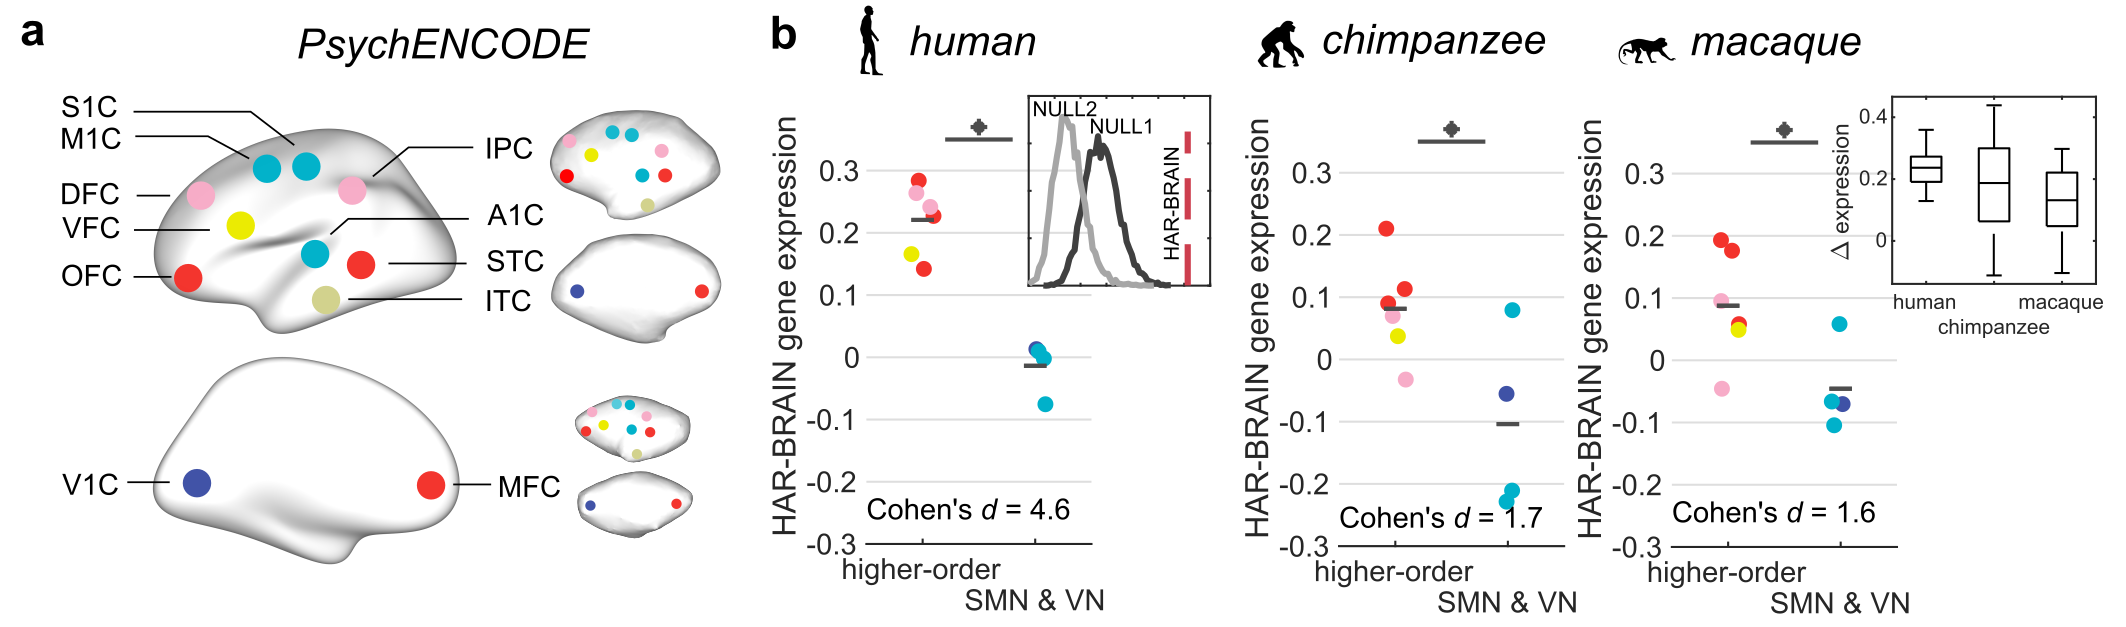
\includegraphics[width=\linewidth]{images/harFig5.png}
    \caption{g Species-homologous brain areas as presented in the PsychENCODE dataset for the human (left), chimpanzee (upper right), and macaque (lower right). h Normalized expression levels of HAR-BRAIN genes in regions of higher-order networks compared to areas of the SMN/VN in humans (p < 0.001, two-sample t test). Largest differences in gene expression are found in humans, with chimpanzees in second place, followed by macaques (p = 0.002, Jonckheere-Terpstra test). Asterisks (*) indicates two-sided p < 0.05, FDR corrected. Central marks denote the mean gene expression. Boxplot center, median; box = 1st-3rd quartiles (Q); lower whisker, Q1 - 1.5 $\times$ interquartile range (IQR); upper whisker, Q3 + 1.5 $\times$ IQR. Colors indicate the assignment of functional networks, as in Fig. 2b. M1C primary motor cortex, S1C primary sensory cortex, IPC inferior parietal cortex, STC superior temporal cortex, ITC inferior temporal cortex, A1C primary auditory cortex, OFC orbital frontal cortex, VFC ventral frontal cortex, DFC dorsal frontal cortex, V1C primary visual cortex, MFC medial frontal cortex. Source data provided as Source Data file}
    \label{harFig5}
\end{figure}


Further evaluation of this cross-species effect showed a significantly decreasing step-wise relationship of differences in HAR-BRAIN gene expression between regions of higher-order networks and the SMN/VN from humans (highest) to chimpanzees and macaques (lowest differentiating expression, Jonckheere-Terpstra test, \pval = 0.002). To reduce the influence of a relatively large variance of expression levels within chimpanzees and macaques (Fig. 3h), we performed a leave-one-out analysis (iteratively leaving out one region at a time) and confirmed a larger mean gene expression difference between cognitive network regions and primary regions in humans in comparison to chimpanzees and macaques (Supplementary Fig. 6). These findings thus suggest that humans display upregulated expression of HAR-BRAIN genes in brain areas involved in cognitive brain function as compared to other primates.

\subsection*{Top strongest differentiating DMN genes}
We continued by investigating the biological properties of genes showing the highest levels of expression in DMN regions out of all genes. For each gene in AHBA, we computed the upregulated level of gene expression in regions of the DMN by calculating the t-score for expressions of the selected gene in regions of the DMN against the rest of the brain. The top 200 highly expressed genes (i.e., genes showing the highest positive t-scores, referred to as DMN genes; all \pval < 0.004) were taken as the DMN’s most differentiating genes (Supplementary Data 3). Out of the top 200 DMN genes, we identified 37 to be HAR genes, particularly including 18 HAR-BRAIN genes, which greatly exceeded the chance level of randomly selecting 37 or 18 out of 20,734 genes (both \pval < 0.001, hypergeometric test). We also examined the top 53 genes with \pval < 0.0014 (partial Bonferroni corrected, see Supplementary Methods) and top 469 genes with \pval < 0.01 (uncorrected), which revealed comparable findings (Supplementary Note 2).

To investigate whether the observed effect was restricted to the DMN, an additional permutation analysis was performed by shuffling region labels and re-computing the top genes for each of these random network assignments. We found the ratio of HAR genes in the set of top DMN genes to be significantly higher than the null condition (\pval < 0.001, 10,000 permutations), which confirmed a dominant role of HAR genes in DMN organization. To further examine potential DMN specificity, we also selected the top 200 genes showing the largest differentiating gene expression in each of the other functional networks compared to the SMN/VN. In contrast to the DMN (revealing 18 overlapping genes with the set of HAR-BRAIN genes), the top 200 gene sets identified by the VAN, DAN, FPN, and LN, comprised, respectively, only 12,8,7 and 7 HAR-BRAIN genes.

Gene-set enrichment analysis on the set of DMN genes using hypergeometric testing in the web-based platform FUMA \citep{watanabe2017functional} showed significant over-representation of DMN genes in Gene Ontology (GO) terms related to cellular components of dendrite (\pval = 2.60 $\times$ 10\textsuperscript{-5}), somatodendritic compartment (\pval = 4.49 $\times$ 10\textsuperscript{-5}), synapse (\pval = 2.15 $\times$ 10\textsuperscript{-4}), perikaryon (\pval = 7.45 $\times$ 10\textsuperscript{-5}) and neuron projection terminus (\pval = 2.26 $\times$ 10\textsuperscript{-4}), as well as molecular functions of neuropeptide hormone activity and calcium activated potassium/cation channel activity (\pval = 1.66 $\times$ 10\textsuperscript{-5} and 1.32 $\times$ 10\textsuperscript{-4}; FDR corrected; Supplementary Table 4).

\subsection*{GWAS on DMN functional activity}
We then wanted to examine whether HAR/HAR-BRAIN genes played a role in inter-subject variation in default-mode functional activity in today's human population. We performed a GWAS on 6,899 participants from the UK Biobank \citep{sudlow2015uk} (see Supplementary Methods) with the amplitude of fMRI time series of the independent component analysis (ICA)-based resting-state networks ("NETMAT amplitudes 25"\citep{elliott2018genome} as described in https://www.fmrib.ox.ac.uk/ukbiobank/) as the phenotypes of interest. Particularly, we focused on the amplitude of the ICA component No.1 that resembles the DMN (referred to as DMN amplitude, Fig. 4a). GWAS results for all single-nucleotide polymorphisms (SNP) with minor allele frequency (MAF) > 0.005 were assessed (Fig. 4b). The quantile-quantile plot showed a linkage disequilibrium score regression [LDSC] intercept of 0.999 (standard error [s.e.] = 0.006), with an inflation level of $\lambda$\textsubscript{GC} = 1.005 and mean $\chi$\textsuperscript{2} statistic = 1.012. LDSC-based SNP heritability [\textit{h}\textsuperscript{2}\textsubscript{SNP}] was 0.09 [s.e. = 0.06]. We observed 3 independent (\textit{r}\textsuperscript{2} < 0.1) genome-wide significant SNPs (\pval < 5 $\times$ 10\textsuperscript{-8}; using linear regression model; Fig. 4b) across 2 genomic loci (Fig. 4c). Furthermore, we annotated 19 significant SNPs (\pval < 5 $\times$ 10\textsuperscript{-8}) with high LD (\textit{r}\textsuperscript{2} $\geq$ 0.6) to the 3 independent SNPs using gene-mapping functions in FUMA \citep{watanabe2017functional} (see Methods section), which resulted in a set of 12 genes (Supplementary Table 5; three genes [\textit{PLCE1}, \textit{NOC3L}, and \textit{SLC35G1}] annotated using brain-related eQTL and Hi-C mappings). Hypergeometric testing \citep{watanabe2017functional} showed significant enrichment of the 12 genes in the GWAS catalog \citep{buniello2018nhgri} reported gene-set "plasma clozapine-norclozapine ratio in treatment-resistant schizophrenia" (\pval = 1.26 $\times$ 10\textsuperscript{-12}; Supplementary Table 6). None of the genes overlapped with HAR-BRAIN genes or the top 200 DMN. One gene (\textit{INPP5A}) denoted as a HAR gene.

We further investigated the potential association of HAR/HAR-BRAIN genes with variations in DMN amplitude using MAGMA linear-regression-based gene-set analysis\citep{de2015magma}. We found HAR-BRAIN genes to be significantly associated with the phenotypic variation in DMN amplitude ($\beta$ = 0.015, \pval  = 0.016, FDR corrected). No significant effect was found for the set of HAR genes ($\beta$ = 0.011, \pval = 0.051; Supplementary Table 7) or DMN genes ($\beta$ = 0.005, \pval = 0.219). An additional conditional gene-set analysis \citep{de2018conditional} including the set of BRAIN genes as a covariate, further showed a significant association of HAR-BRAIN genes with variations in DMN amplitude ($\beta$ = 0.014, \pval = 0.022; HAR genes: $\beta$ = 0.011, \pval = 0.055; Fig. 4e). Furthermore, no significant effect was observed when we examined the association between HAR-BRAIN genes and amplitude of other ICA components resembling the rest of the functional networks (\pval > 0.09; Fig. 4f and Supplementary Table 8), implicating a specific role of HAR-BRAIN genes in genetic variations of DMN functional activity. Using the normalized DMN amplitude (corrected for the mean amplitude across all networks) as the phenotype of interest showed similar results (HAR genes: $\beta$ = 0.018, \pval = 0.003; HAR-BRAIN genes: $\beta$ = 0.020, \pval = 0.002; Supplementary Fig. 7).

Stratified LDSC analysis\citep{finucane2015partitioning} did not result in findings of significant enrichment of genetic variance of DMN functional activity explained by SNPs overlapping with HAR regions. This is likely related to HARs occupying relatively small regions in the whole genome with a mean length of only 256 base pairs (Supplementary Fig. 8), which limits statistical power to perform such post-hoc analyses. The relatively large s.e. of the SNP heritability might be related to the limited sample size.

\begin{figure}[H]
    \centering
    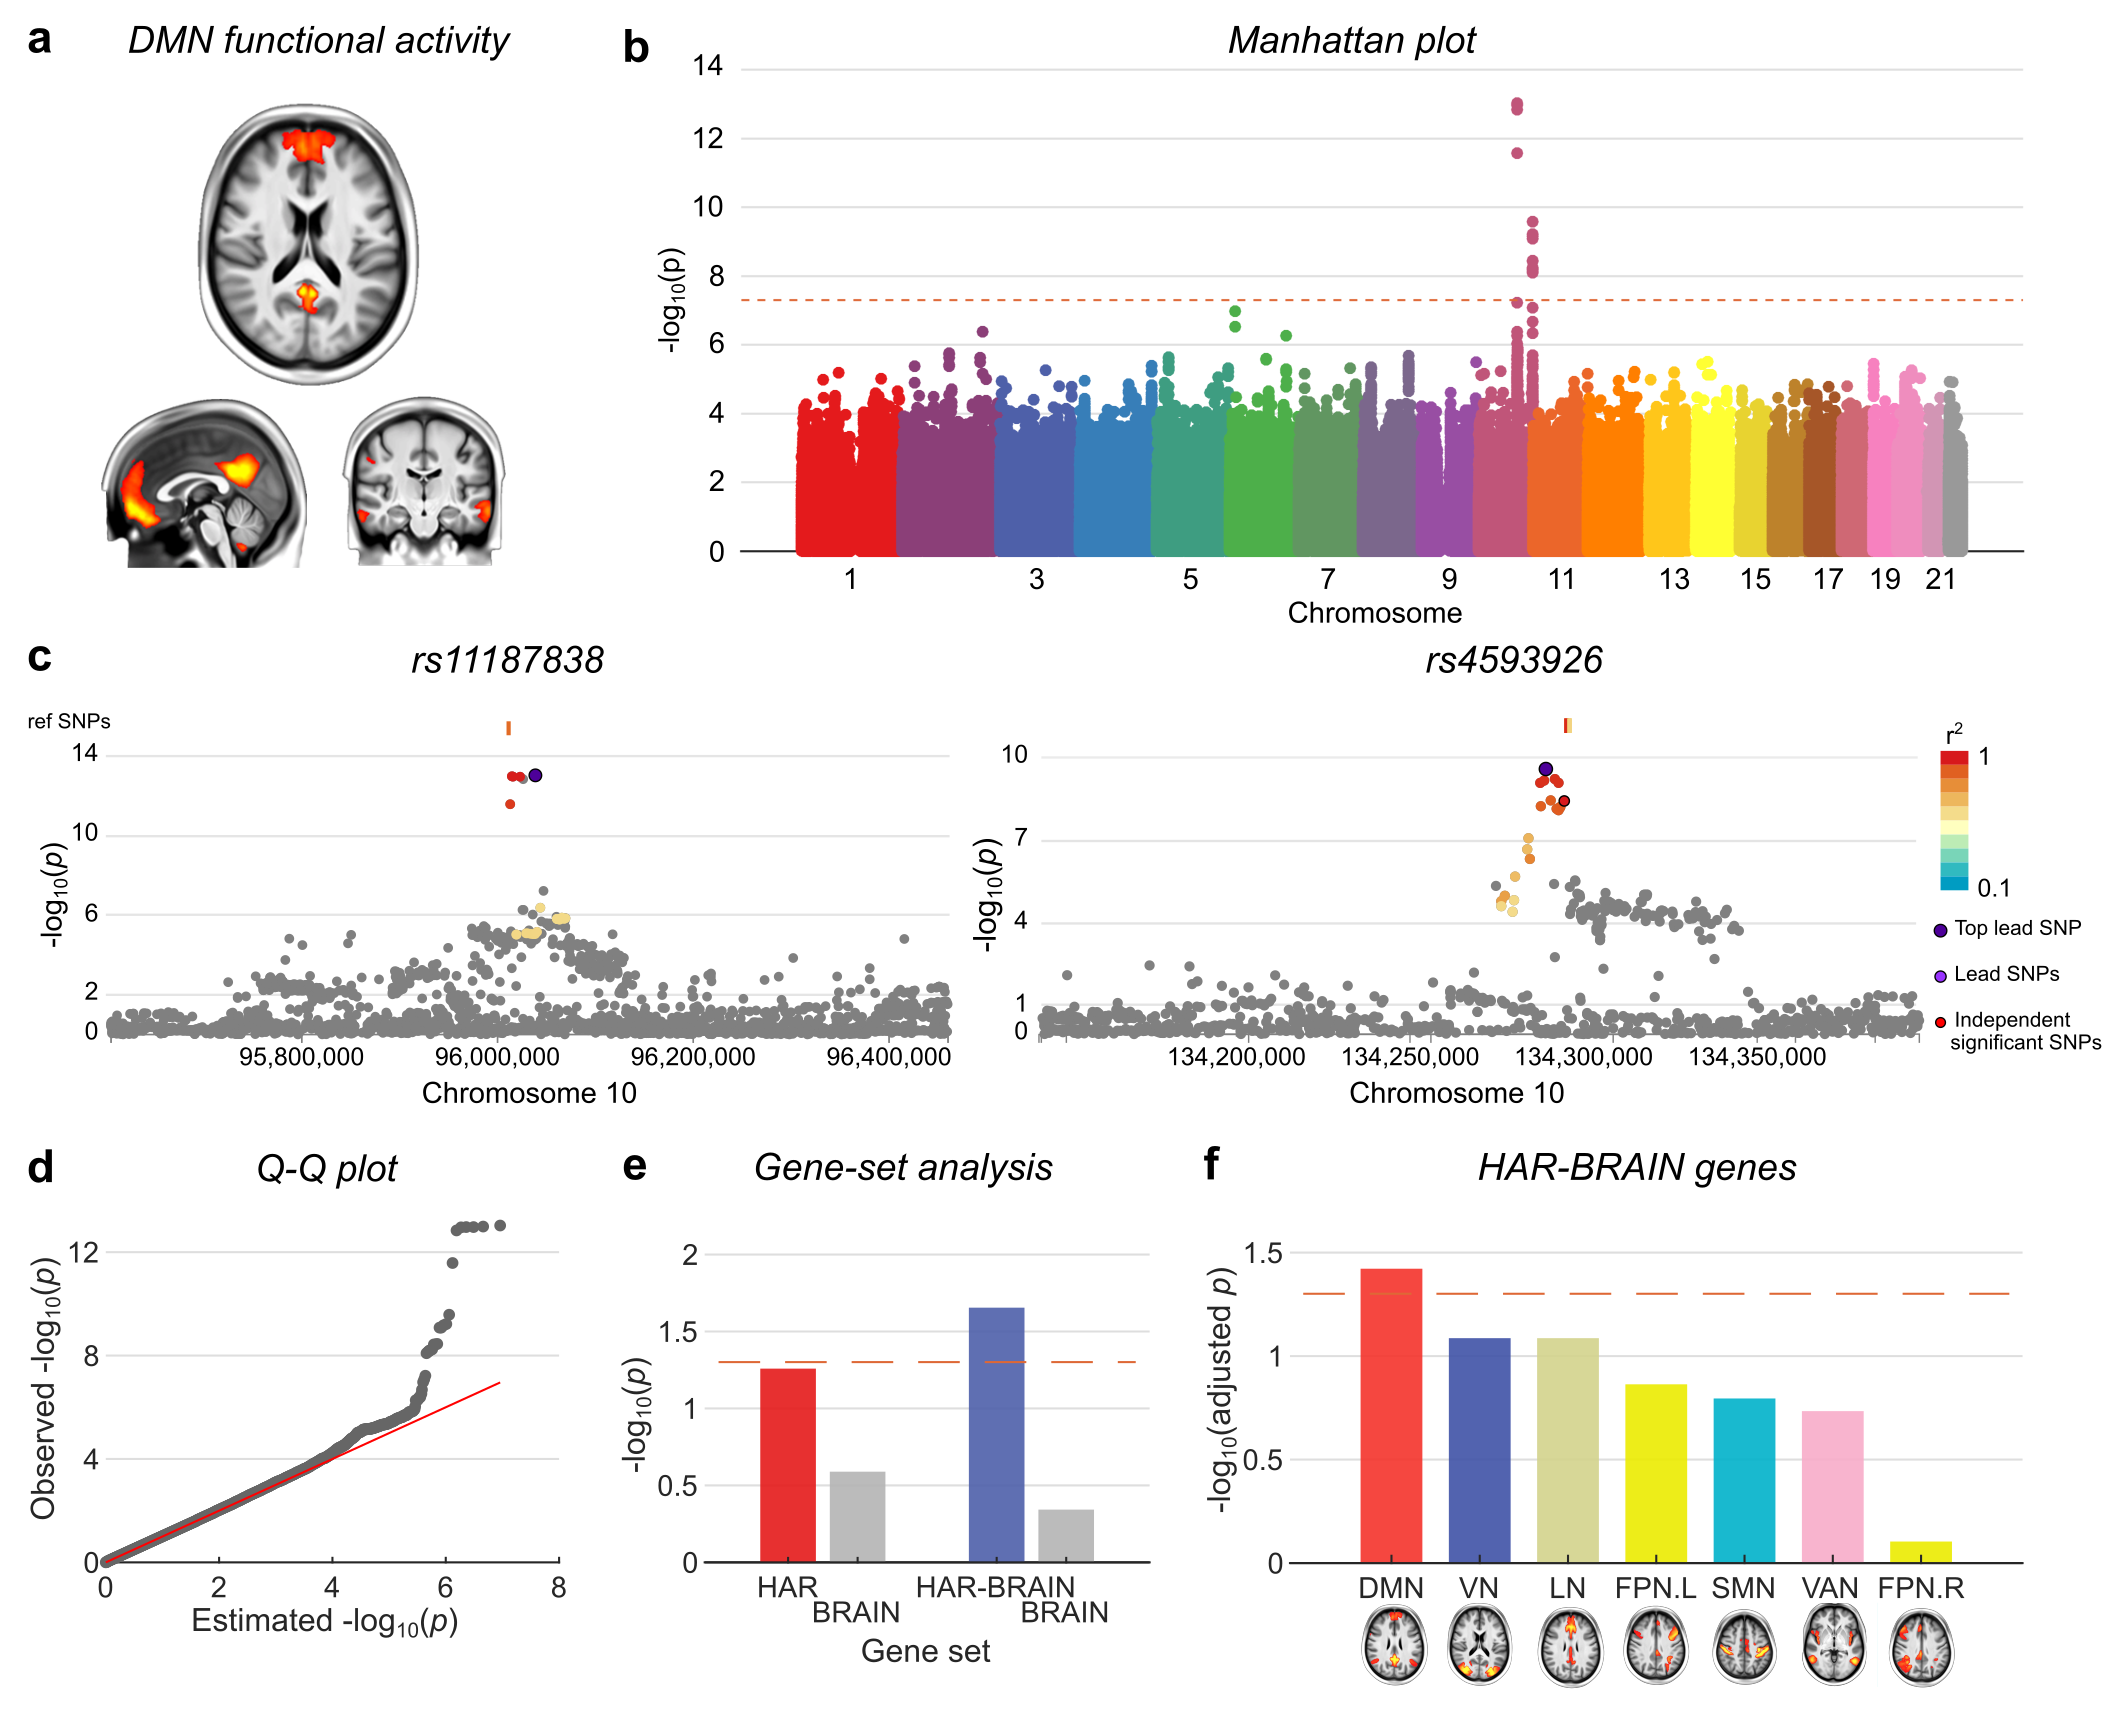
\includegraphics[width=\linewidth]{images/harFig6.png}
    \caption{GWAS on DMN activity. a DMN component. b GWAS Manhattan plot showing -log10-transformed two-tailed p-value for all SNP (y-axis) and base-pair positions along the chromosomes (x-axis). Dotted red line indicates Bonferroni-corrected genome-wide significance (p-value < 5 $\times$ 10-8). c Regional plots of the two genomic loci (left, lead SNP: rs11187838 and right, lead SNP: rs4593926). d Q-Q plot of SNP-based p-value in panel b. Observed -log10 transformed two-tailed p-values of associations with DMN functional activity are plotted against expected null p-values for all SNPs in the GWAS. e MAGMA conditional gene-set analysis. -log10-transformed p-values of the associations between HAR/HAR-BRAIN genes and DMN functional activity conditional upon BRAIN genes. Dashed line indicates p = 0.05. f MAGMA gene-set analysis on HAR-BRAIN genes and other "NETMAT amplitude 25" phenotypes representing functional activity in the other functional networks (-log10-transformed adjusted p-values, FDR corrected). Colors indicate the assignment of functional networks, as in Fig. 2b. Dashed line indicates adjusted p = 0.05}
    \label{harFig6}
\end{figure}

\subsection*{HAR genes, cognitive abilities, and psychiatric disorders}

We then examined the potential role of HAR/HAR-BRAIN and DMN genes in human cognition by cross-referencing these genes with a recent GWAS meta-analysis on intelligence (\textit{h}\textsuperscript{2}\textsubscript{SNP} = 0.184 [s.e. = 0.008]) performed on 269,867 individuals \citep{Savage2018GenomewideAM}. Gene-set analysis \citep{de2015magma} revealed both sets of HAR and HAR-BRAIN genes to be significantly associated with individual variations in intelligence (HAR: $\beta$ = 0.058, \pval = 5.43 $\times$ 10\textsuperscript{-10}; HAR-BRAIN: $\beta$ = 0.075, \pval = 1.22 $\times$ 10\textsuperscript{-15}; Supplementary Table 7). Conditional gene-set analysis \citep{de2018conditional} including BRAIN genes as a covariate further confirmed a significant association of both HAR and HAR-BRAIN genes with intelligence (HAR: $\beta$ = 0.056, \pval = 1.60 $\times$ 10\textsuperscript{-9}; HAR-BRAIN: $\beta$ = 0.060, \pval = 6.34 $\times$ 10\textsuperscript{-10}). Intelligence was not found to be specifically associated with the total set of DMN genes ($\beta$ = 0.012, \pval = 0.061), but a significant effect was observed for the subset of 37 intersected HAR-DMN genes ($\beta$ = 0.022, \pval = 0.009, FDR corrected).

We next linked HAR/HAR-BRAIN and DMN genes to genetic effects on social behavior, which is thought to be more advanced in humans than in other primate species \citep{tomasello2010ape}. Summary statistics of the trait “Frequency of friend/family visits” (\textit{h}\textsuperscript{2}\textsubscript{SNP} = 0.035 [s.e. = 0.002]) based on a GWAS analysis on 383,941 individuals in the UK Biobank were obtained from the GWAS ATLAS web tool \citep{Watanabe2019AGO} (http://atlas.ctglab.nl, ID 3216). HAR/HAR-BRAIN genes were found to be significantly associated with this trait (HAR: $\beta$ = 0.037, \pval = 1.24 $\times$ 10\textsuperscript{-7}; HAR-BRAIN: $\beta$ = 0.039, \pval = 1.01 $\times$ 10\textsuperscript{-7}; Supplementary Table 7), with effects unrelated to the set of BRAIN genes (HAR: $\beta$ = 0.037, \pval = 1.73 $\times$ 10\textsuperscript{-7}; HAR-BRAIN: $\beta$ = 0.036, \pval = 2.63 $\times$ 10\textsuperscript{-6}). Furthermore, DMN genes were also significantly associated with individual variation in sociability ($\beta$ = 0.012, \pval = 0.024; HAR-DMN genes: $\beta$ = 0.014, \pval = 0.022, FDR corrected).

We also examined the potential association of HAR/HAR-BRAIN and DMN genes with schizophrenia, a disorder hypothesized to relate to human brain evolution \citep{crow1997schizophrenia,Heuvel2019EvolutionaryMI}. We used the summary statistics of a GWAS in 33,426 schizophrenia patients and 54,065 healthy controls (\textit{h}\textsuperscript{2}\textsubscript{SNP} = 0.187 [0.008])34 provided by the Psychiatric Genomics Consortium (http://www.med.unc.edu/pgc/). We observed HAR/HAR-BRAIN genes to be significantly associated with genetic variants in schizophrenia (HAR: $\beta$ = 0.019, \pval = 0.013; HAR-BRAIN: $\beta$ = 0.043, \pval = 5.06 $\times$ 10\textsuperscript{-7}; Supplementary Table 7). These results remained significant in the conditional gene-set analysis with BRAIN genes taken as a covariate (HAR: $\beta$ = 0.017, \pval = 0.023; HAR-BRAIN: $\beta$ = 0.028, \pval = 0.001). DMN genes were not found to be significantly associated with schizophrenia ($\beta$ = 0.011, \pval = 0.067; HAR-DMN genes: $\beta$ = 0.005, \pval = 0.261). In addition to common variations indicated by GWAS, we further examined the enrichment of HAR/HAR-BRAIN and DMN genes in rare variants of brain disorders using the NPdenovo database (http://www.wzgenomics.cn/NPdenovo/) \citep{li2016genes}. Hypergeometric testing showed HAR and HAR-BRAIN genes to be significantly enriched in risk genes of ASD (\pval  < 0.001 and \pval = 0.005, separately) and schizophrenia (\pval < 0.001 and \pval = 0.008, separately; FDR corrected). DMN genes also showed significant enrichment in risk genes of ASD (\pval = 0.004), but not schizophrenia (\pval = 0.264; Supplementary Fig. 9).

We also examined a potential association of HAR-BRAIN genes with brain changes related to psychiatric disorders. We used data from voxel-based morphometry (VBM) studies in five psychiatric brain disorders (schizophrenia, bipolar disorder, ASD, major depressive disorder [MDD] and obsessive-compulsive disorder [OCD]) and created a cortical map describing the distribution of cortical volume changes of these five psychiatric disorders (including in total of 260 VBM studies). The spatial pattern of disorder involvement across the cortex was significantly associated with the gene expression pattern of HAR-BRAIN genes (\rvaldf(55) = 0.437, \pval < 0.001, with the cortical volume controlled; Fig. 5; \rvaldf(55) = 0.221, \pval = 0.098 for HAR genes), an effect significantly exceeding the effect obtained by BRAIN genes (\pval = 0.022) and ECE genes (\pval < 0.001, 10,000 permutations). For an out-group analysis, the cortical pattern of HAR-BRAIN gene expression did not correlate to the disease map of five alternative, non-psychiatric disorders (amyotrophic lateral sclerosis, stroke, alcoholism, insomnia, fibromyalgia; \rvaldf = 0.141, \pval = 0.302).

\begin{figure}[h]
    \centering
    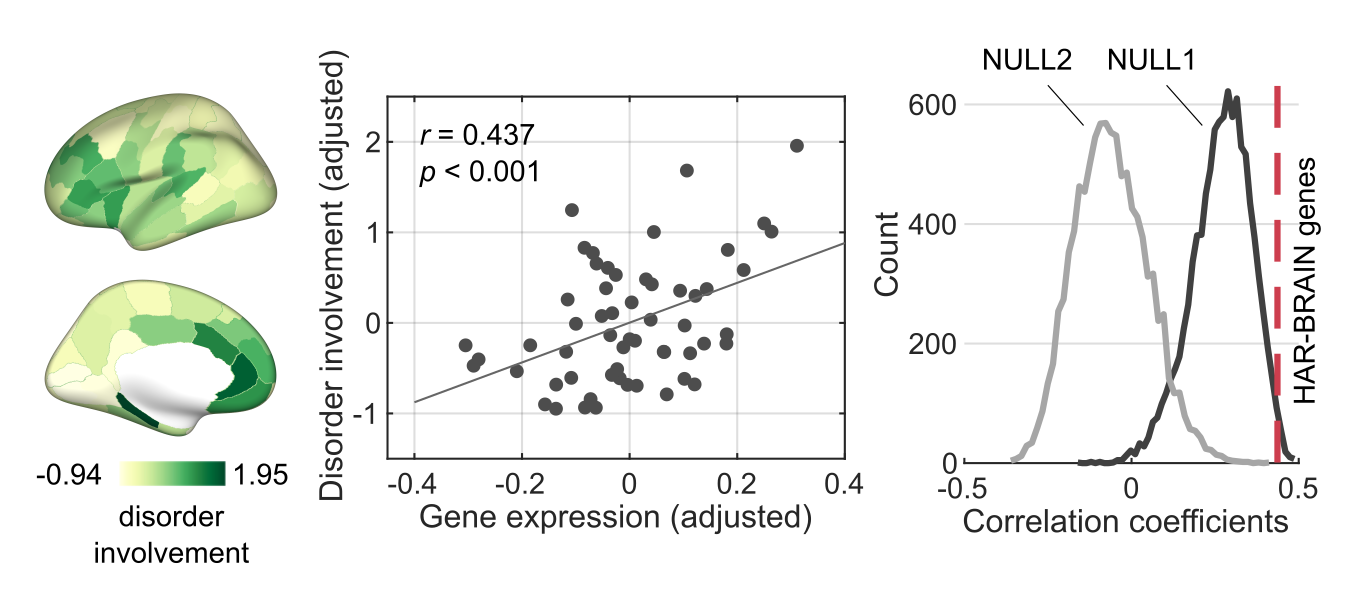
\includegraphics[width=\linewidth]{images/harFig7.png}
    \caption{Cortical disorder involvement and HAR-BRAIN gene expression. Left panel shows brain maps of cortical involvement across five major psychiatric disorders (e.g., schizophrenia, bipolar disorder, autism spectrum disorder, major depression, and obsessive-compulsive disorder). Middle panel shows correlation between HAR-BRAIN gene expression and disorder involvement (Pearson's r = 0.437, p < 0.001; corrected for cortical volume), and right panel shows the comparison of the correlation coefficient to null distributions generated by random BRAIN (NULL1; p = 0.022) and ECE genes (NULL2; p < 0.001, permutation test, 10,000 permutations). Source data provided as Source Data file}
    \label{harFig7}
\end{figure}

\section*{Discussion}
Our combined comparative neuroimaging and genetic findings provide evidence of evolutionary changes in the human genome to have played a central function in the expansion and cortical organization of cognitive functional networks in the human brain, potentially in service of specialization of higher-order cognitive function in human evolution.

Our results show high levels of cortical expansion in regions of both the FPN and DMN in humans. This is compatible with prior observations of cortical expansion between macaque and human \citep{hill2010similar}, showing large expansion of associative prefrontal, temporal, and parietal areas in the human brain \citep{hill2010similar,donahue2018quantitative}. This evolutionary expansion pattern has been suggested to overlap with the pattern of cortical variation in today’s human population \citep{reardon2018normative}, suggesting larger brains to display relatively larger multi-modal associative areas, variation further linked to inter-subject variation in cognitive abilities \citep{Ryu256313}. Our observations of high expression of HAR genes in these brain areas now suggest that genes linked to hominization may have had a special role in the process of cortical development of these multimodal association areas.

Our comparative analyses further show that genes associated with human brain evolution (HAR-BRAIN genes) are not equally expressed in all cortical areas but rather are more expressed in areas related to higher-order cognitive processing. HAR genes, representing conserved loci with elevated divergence in humans \citep{pollard2006rna,doan2016mutations}, have been argued to function as important neuronal enhancers \citep{Ryu256313} and to be key players in biological processes of nervous system development and neurogenesis, amongst others (Supplementary Table 9). HAR genes are enriched in human-evolved elements that converge on specific cell types and laminae involved in brain development and cerebral cortical expansion in the primate lineage \citep{won2019human} and are suggested to be particularly expressed in supragranular cortical layers important for forming cortico-cortical connectivity \citep{won2019human}. Our findings of high expression of HAR genes in central cognitive networks, and most pronounced in the DMN, may thus reflect enhanced complexity of cognitive cortical areas and circuits in human brain evolution \citep{elston2001pyramidal,jacobs2001regional}.

Our results corroborate previous observations of a strong link between aspects of cellular and macroscale connectivity \citep{vandenheuvel2019multi,scholtens2014linking}. Association areas show transcriptional profiles enriched for genes specific to the organization of supragranular layers \citep{vertes2016gene}, with the spatial layout of functional networks captured by coupled transcription profiles of genes enriched in supragranular layers \citep{krienen2016transcriptional} and genes related to ion channel activity and synaptic function \citep{richiardi2015correlated}. These observations are further in line with the notion of genes related to the resting-state brain activity of the DMN to display greater expression in neurons \citep{wang2015correspondence}. Moreover, our observation of upregulated HAR-BRAIN gene expression in cognitive networks in humans implicates an evolutionarily enhanced complexity of neuronal connectivity in cognitive networks. This might be potentially further related to humans having a longer period of neuronal progenitor expansion compared with chimpanzees and macaques contributing to a differentiated neuronal number and cortical size \citep{otani20162d}.

Some of the genes found at the intersection of HAR, BRAIN, and DMN genes directly relate to the development of the human central nervous system. For example, CDH8, CDH9, and CDH10 are involved in synaptic adhesion, axon outgrowth, and guidance49, and play a role in ASD \citep{redies2012cadherins}. CBLN1 is important for synapse integrity and synaptic plasticity together with NRXN1 and GRID2 \citep{hirai2005cbln1}. CA10 is believed to be central in the development of the central neural system by coordinating neurexins, which are presynaptic cell-adhesion molecules that bind to diverse postsynaptic ligands and who are linked to several neuropsychiatric disorders \citep{sterky2017carbonic}. KCNB2 is known to be essential in regulating neurotransmitter release and neuronal excitability \citep{coetzee1999molecular}.

Our findings show that genes highly expressed in the DMN contain genetic variants related to human intellectual ability and sociability. This is compatible with twin studies showing a genetic correlation between IQ and gray matter morphology of DMN regions like the medial frontal cortex and parahippocampal gyrus \citep{hulshoff2006van}. The DMN has been argued to be important for human self-projection abilities that include planning the future \citep{suddendorf2009mental}, theory of mind, and navigation \citep{buckner2007self}, of which humans show a higher complexity compared to chimpanzees \citep{corballis2013mental}. This central cognitive system comprises highly connected network hubs like the precuneus and inferior parietal lobule \citep{van_den_heuvel_network_2013}, regions involved in multimodal information integration \citep{barbey2018network}, a key aspect of higher-order cognitive brain function. The observation of an association between the spatial pattern of HAR expression and cortical expansion on the one hand, and a significant involvement of HAR genes in genetic variation related to intelligence and social behavior on the other, suggests that the expansion of highly connected hub areas in support of higher-order brain function has been an important driving factor of human brain evolution.

Evolutionary pressure on cognitive networks subserving higher-order brain functions may have been accompanied by an increased risk of brain dysfunction \citep{crow1997schizophrenia,Heuvel2019EvolutionaryMI}. Our comparative findings provide evidence for this hypothesis, with genes important for human brain evolution found to play a role in the development of psychiatric disorders. The pattern of cortical expression of HAR-BRAIN genes shows significant overlap with the pattern of cortical involvement across mental disorders, with particular involvement of lateral and medial prefrontal cortices. These are key 'brain hubs' and components of higher-order networks identified to be generally implicated in the anatomy of a wide range of brain disorders58. Our findings further suggest HAR and DMN genes to significantly relate to the genetic architecture for schizophrenia and autism, disorders that are often reported to involve disturbed DMN functional connectivity \citep{padmanabhan2017default,Lange2019SharedVF}. These findings are consistent with reported genetic associations between the DMN and psychiatric disorders \citep{meda2014multivariate} and support the notion of genes related to evolutionary adaptations and brain development to potentially contribute to default-mode network involvement in brain disorders \citep{meda2014multivariate}.

Several methodological points have to be discussed. We used predefined functional networks to link data from distinct modalities. Network divisions may overlook functional heterogeneity across cortical regions and participation of brain regions in multiple networks, and several other spatial variations of networks are equally viable \citep{smith2009correspondence} (see Supplementary Note 5 for alternative definitions of networks, Supplementary Fig. 10-11). Second, the set of HAR genes as used in this study was selected 'as-is' from the study of Doan et al. \citep{doan2016mutations}. HAR-associated genes were labeled as those where HARs are within the introns, within or near (less than 1 kb) 5' and 3' UTRs, or are the closest flanking gene that was less than 2.1 mb away (with 70\% being less than 500 kb away) \citep{doan2016mutations}. Other mapping approaches can be used to identify and further specify HAR gene sets linked to specific functions. We examined alternative sets of 196 genes mapped from HAR using brain-related Hi-C and eQTL datasets from the PsychENCODE Consortium \citep{wang2018comprehensive}, and a set of 396 genes related to ASD-linked HAR mutations identified using massively parallel reporter assays \citep{doan2016mutations}. These alternative selections and allocations of HAR genes revealed highly consistent findings (data presented in detail in Supplementary Note 1).

Our comparative study shows that recent changes in our genome have played a central role in the expansion and function of higher-order cognitive networks in the human brain. Our findings suggest that expansion of higher-order functional networks and their cognitive properties have potentially been an important locus of change in recent human brain evolution.

\section*{Methods}
\subsection*{Cortical expansion}
In vivo MRI data from 29 adult chimpanzees and 50 adult human subjects were analyzed (see Supplementary Methods for details). Data of chimpanzees were acquired under protocols approved by the YNPRC and the Emory University Institutional Animal Care and Use Committee (IACUC, approval \#: YER2001206) (see also Ethics statement). MRI data of humans were obtained from the Human Connectome Project (https://www.humanconnectome.org). T1-weighted scans of chimpanzees and humans were processed using FreeSurfer (v5.3.0; https://surfer.nmr.mgh.harvard.edu/) for tissue classification, cortical ribbon reconstruction, and brain parcellation. Pial surface reconstructions were used for vertex-to-vertex mapping across chimpanzee and humans and subsequent computation of vertex-wise and region-wise expansion (114-region subdivision of the Desikan-Killiany atlas [DK-114] \citep{DESIKAN2006968,CAMMOUN2012386}, 57 per hemisphere; see Supplementary Methods and Supplementary Figs. 12-13). Vertex-wise and region-wise expansion maps are available at https://www.connectomelab.nl/downloads. Validation analysis was performed using the chimpanzee-human BB38 atlas that describes homologous cortical regions between two species \citep{Heuvel2019EvolutionaryMI} (Supplementary Fig. 14).

\subsection*{Gene expression}
\subsubsection*{AHBA}
Cortical gene expression patterns were taken from the transcriptomic data of the Allen Human Brain Atlas (AHBA, http://human.brain-map.org/static/download), including a detailed dataset of microarray gene expression data from brain samples of six human donors (all without a history of neuropsychiatric or neuropathological disorders, demographics tabulated in Supplementary Table 10). Data included expression levels of 20,734 genes represented by 58,692 probes for each cortical region of the left hemisphere \citep{Romme2017ConnectomeDA}. Tissue samples were spatially mapped to each of the cortical regions of the FreeSurfer DK-114 atlas \citep{DESIKAN2006968,CAMMOUN2012386}, based on their distance to the nearest voxel within the cortical ribbon of MNI 152 template (and BB38 atlas for validation, see Supplementary Note 4). Samples were normalized to Z scores and averaged across regions (see Supplementary Methods), resulting in a subject $\times$ region $\times$ gene (6 $\times$ 57 $\times$ 20,734) data matrix. Normalized gene expression data was averaged across individual datasets to obtain a group level gene expression matrix of the size of 57 $\times$ 20,734.

\subsubsection*{PsychENCODE}
Comparative cortical transcription data were obtained from the PsychENCODE database (http://evolution.psychencode.org/) \citep{sousa2017molecular}, describing batch-corrected, normalized expression levels of 16,463 genes for 11 comparable cortical areas of the human (6 subjects), chimpanzee (5 subjects), and macaque brain (5 subjects, all age and gender controlled and corrected for batch effects22, see Supplementary Methods, Supplementary Table 11, and ref. \citep{sousa2017molecular} for details). Gene expression data were normalized to Z scores across cortical regions within each dataset, resulting in three gene expression matrices (one for each species) of the size of n $\times$ 11 $\times$ 16,463 (n = 6/5/5 for human/chimpanzee/macaque). Data were averaged across individual datasets to obtain a group level gene expression matrix of the size of 11 $\times$ 16,463 for each species.

\subsubsection*{HAR genes}
Genes located in human accelerated regions (HARs) of the genome were taken as presented by comparative genome analysis representing genomic loci with accelerated divergence in humans \citep{doan2016mutations}. A total number of 2737 human accelerated regions were identified, representing 2143 HAR-associated genes \citep{doan2016mutations}. One thousand seven hundred and eleven HAR-associated genes were described in the AHBA dataset and used in our analyses, referred to as HAR genes.

\subsubsection*{BRAIN genes}
BRAIN genes were selected as the set of genes commonly expressed in human brain tissue using the Genotype-Tissue Expression (GTEx) database (data source: GTEx Analysis Release V6p; https://www.gtexportal.org/). The GTEx portal contains 56,238 gene expression profiles in 53 body sites collected from 7333 postmortem samples in 449 individuals. From these 56,238 genes, a total number of 2823 genes were identified as BRAIN genes showing significantly higher expressions in brain sites than non-brain sites (one-sided t-test and an FDR corrected \textit{q} < 0.05 were used). Four hundred and five of these 2823 genes overlapped with the set of HAR genes, referred to as HAR-BRAIN genes.

\subsection*{DMN genes}
For each of the 20,734 AHBA genes, a two-sided two-sample t-test was performed between expression levels of regions of the DMN and regions of the other resting-state networks. Genes showing the top 200 largest t-scores (showing \pval < 0.004, uncorrected) were selected and referred to as DMN genes (consistent results were obtained for the set of genes reaching \pval < 0.05, corrected for multiple comparisons and alternatively the set of genes reaching \pval < 0.01 without correction; see Supplementary Note 2 and Supplementary Tables 12-13). Enrichment of HAR genes in top DMN genes was statistically evaluated using hypergeometric test. Gene-set analysis was performed for the set of DMN genes by means of the hypergeometric test implemented in the GENE2FUNC function in FUMA (http://fuma.ctglab.nl) \citep{watanabe2017functional} (see Supplementary Methods).

\subsection*{DMN GWAS}
GWAS was performed on 6899 participants from the UK Biobank (July 2017 release; http://www.ukbiobank.ac.uk; including individuals of European ancestry, relatives excluded). fMRI amplitude of seven ICA-based resting-state networks (described as "NETMAT amplitudes 25" in http://big.stats.ox.ac.uk/; UK Biobank field ID: 25754; for a detailed description, see refs. \citep{Miller2016MultimodalPB,elliott2018genome} and https://www.fmrib.ox.ac.uk/ukbiobank) were taken as phenotypes of interest. We focused on the phenotype "NETMAT amplitudes 25(01)", describing ICA component \#1 resembling the DMN. In addition, ICA component \#2, \#3, \#5, \#6, \#10, and \#14 were examined, respectively, reflecting the VN, VAN, FPN.R, FPN.L, SMN, and LN. GWAS was conducted in PLINK v2.00 \citep{Purcell2007PLINKAT}, using an additive linear regression model controlling for covariates of age, sex, twenty European-based ancestry principal components, genotyping array, and total brain volume (derived from the T1 image, linearly transformed to mean zero and variance one). Stringent quality control measures were applied to the summary statistics of the GWAS (see Supplementary Methods and ref. \citep{Savage2018GenomewideAM} for a detailed description of the used procedures). SNP-based results were mapped and annotated using positional mapping, eQTL mapping, and chromatin interaction mapping as implemented in the SNP2GENE function in FUMA \citep{watanabe2017functional}. MAGMA gene-set analysis was used to examine the association of HAR/HAR-BRAIN/DMN genes with phenotypic variations \citep{watanabe2017functional,de2015magma}.

\subsection*{Gene-set analysis}
SNP-based summary statistics of three GWAS were obtained, including (1) a recent GWAS meta-analysis on intelligence in 269,867 individuals \citep{Savage2018GenomewideAM}; (2) a GWAS of a social interaction related trait, "Frequency of friend/family visits", in 383,941 individuals in the UK Biobank \citep{Watanabe2019AGO} (field ID: 1031; GWAS ATLAS web tool, http://atlas.ctglab.nl/traitDB/3216); (3) a GWAS in 33,426 schizophrenia patients and 54,065 healthy controls34 as provided by the Psychiatric Genomics Consortium (http://www.med.unc.edu/pgc/). Gene annotation was performed using MAGMA \citep{de2015magma}, providing gene-based p-values and effect sizes that are non-directional and reflect both positive and negative direction given phenotypic variants. Gene-set analysis was performed based on a linear regression model implemented in MAGMA \citep{de2015magma} to examine to what extent HAR/HAR-BRAIN and DMN genes are associated with phenotypic variation. Results reaching an FDR corrected \textit{q} < 0.05 were taken as statistically significant (corrected for all 20 tested associations). Conditional gene-set analysis \citep{de2018conditional} was used to control for the effect of BRAIN genes.

\subsection*{Cortical involvement in psychiatric disorders}
The BrainMap database was used to assess cortical involvement across five major psychiatric disorders (schizophrenia, bipolar disorder, ASD, MDD, and OCD, including in total of 260 studies) (http://www.brainmap.org). Disease voxel-based morphometry (VBM) data of 260 case-control studies present in BrainMap were extracted using the Sleuth toolbox \citep{Fox2002MappingCA} and meta-analyses were conducted for each disorder using the GingerALE toolbox \citep{Eickhoff2009CoordinatebasedAL}. Resulting brain maps of activation likelihood estimation (ALE) were registered to the MNI 152 template and regional ALE was computed by averaging ALEs of all voxels within each cortical region of the DK-114 atlas. Regional averaged ALE scores were transformed to Z scores and averaged into a cross-disorder cortical involvement map describing per region the level of involvement across five major psychiatric disorders (see Supplementary Methods).

\subsection*{Statistical analysis}
Pearson's correlation was used to examine the association of the profile of cortical gene expression with the pattern of chimpanzee-to-human cortical expansion. Two-sided two-sample t-test was used to statistically test the difference in evolutionary cortical expansion and mean gene expression of HAR and HAR-BRAIN genes between regions of higher-order cognitive networks (e.g., the DMN, FPN, and VAN) and regions of the SMN/VN. Similar analysis was conducted between each of the functional networks and the rest of the brain. Results reaching an FDR corrected \textit{q} < 0.05 were taken as statistically significant (corrected for eight tests in each analysis). Cohen's d was computed, as the difference between two means divided by a standard deviation, to indicate the effect size. Permutation testing (10,000 permutations) was used to differentiate effects of HAR-BRAIN genes from effects of general BRAIN genes (referred to as NULL1) and genes associated with evolutionarily conserved elements of the human genome (ECE genes, referred to as NULL2). ECE genes were obtained from evolutionarily conserved elements in the human genome with length larger than 200 base pairs as described in ref. \citep{lindblad2011high} and were mapped to genes when they fall inside the genomic location provided by the gene \citep{de2015magma}, resulting in a set of 9125 genes. For each permutation (for NULL1 and NULL2), 415 genes (the same size as the number of HAR-BRAIN genes) were randomly selected from the pool of 2979 BRAIN genes or 9125 ECE genes, separately, and the same statistics (e.g., Pearson's correlation or t-test) were computed for this random set to generate an empirical null-distribution (i.e., noted as the NULL1 distribution for BRAIN genes and NULL2 distribution for ECE genes). The original effects were assigned a two-sided p-value by comparing to the null-distributions, according to the proportion (P) of random permutations that exceeded the original statistics of HAR-BRAIN genes (p = P $\times$ 2 if P < 0.5, otherwise p = (1 - P) $\times$ 2).

\printbibliography[heading=subbibliography]
\end{refsection}

\begin{refsection}
\newpage
\section*{Supplementary Information}
\subsection*{Supplementary Methods}
\subsubsection*{MRI data}
We calculated cortical expansion using in vivo MRI data from 29 chimpanzees (Pan troglodytes; age: 30.2 $\pm$ 12.6, all female) and 30 humans (Homo sapiens; age: 29.8 $\pm$ 3.2 years; all female). Chimpanzees were accommodated at the Yerkes National Primate Research Center (YNPRC) in Atlanta, Georgia. All procedures were implemented under protocols approved by the YNPRC and the Emory University Institutional Animal Care and Use Committee (IACUC, approval \#: YER-2001206). No new MRI data was acquired for this study. All chimpanzee MRIs were obtained from a data archive of scans obtained prior to the 2015 implementation of U.S. Fish and Wildlife Service and National Institutes of Health regulations governing research with chimpanzees. All the scans reported in this publication were completed by the end of 2012. All MRI scans are part of the National Chimpanzee Brain Resource (http://www.chimpanzeebrain.org).

Chimpanzee MRI scans were collected from chimpanzees under anesthesia with isoflurane (1\%) (protocols described in detail in 1). Chimpanzees were immobilized with ketamine (2-6 mg/kg). Constant observation was given by veterinary staff for chimpanzees before, during, and after scanning. Head motion was minimized using foam cushion and elastic straps. A standard circularly polarized (CP) birdcage coil was used because they did not fit the standard phase-array coil designed for humans. T1-weighted MPRAGE imaging of all chimpanzees was obtained on two Siemens 3T Trio Tim Scanners (Siemens Medical System, Malvern, PA) with the following parameters: slice thickness = 0.8 mm, voxel size = 0.8 $\times$ 0.8 $\times$ 0.8 mm, TR = 2,600 ms, TE = 3.06 ms, matrix size = 256 $\times$ 256 $\times$ 192, FOV = 224 $\times$ 224, flip angle = 8 degree, scanning time = 16 min.

Data of human subjects were randomly selected from the Q3 data release of the Human Connectome Project (HCP, http://www.humanconnectomeproject.org/)2. Human MRI scans were acquired on a Siemens Skyra 3T scanner (Siemens Medical System, Malvern, PA) with a customized SC72 gradient insert2. T1-weighted MPRAGE images were collected with following scanning parameters: voxel size = 0.7 $\times$ 0.7 $\times$ 0.7 mm, TR = 2400 ms, TE = 2.14 ms, matrix = 320, 256 sagittal slices, slice thickness = 0.7 mm, FOV = 224 $\times$ 224, flip angle = 8 degree, scanning time = 7:40 min.

\subsubsection*{MRI processing}
Chimpanzee and human T1-weighted MRI data were processed in the FreeSurfer software\textsuperscript{3, 4} for brain tissue segmentation and cortical mantle reconstruction. Inspired by a recent human-chimpanzee morphological comparison based on FreeSurfer\textsuperscript{5}, chimpanzee-to-human cortical expansion was computed as follows. Individual reconstructed pial surfaces of both chimpanzees and humans were re-meshed to an identical number of vertices. FreeSurfer inflated the white matter - gray matter surface of each subject to a sphere, and registered the sphere to the standard reference ($\$$ FS\_HOME/average/?h.average.curvature.filled.buckner40.tif) by aligning the curvature data, resulting in a surface file of the registered sphere. Next, for each vertex \textit{i} (the target vertex) on the registered sphere of the fsaverage, we extracted the face (i.e., a triangle formed by three vertices) comprising the location of vertex \textit{i} on the registered sphere of each subject. To do this, we used Barycentric coordinates:

\[ P_{i}= [x_{i}, y_{i}, z_{i}] \ \ [1] \]

\[  \left[ \begin{matrix}
u\\
v\\
w\\
\end{matrix}
 \right]  \times  \left[ \begin{matrix}
P_{1}\text{, 1}\\
P_{2},1\\
P_{3},1\\
\end{matrix}
 \right] = \left[ P_{t}\text{, 1} \right] \ \ [2] \] \\

where \textbf{P}\textit{\textsubscript{i}} is a vector of coordinates of a vertex \textit{i}, \textbf{P}\textsubscript{1}, \textbf{P}\textit{\textsubscript{2}}, \textbf{P}\textsubscript{3} are coordinates of three vertices forming a face, \textbf{P}\textit{\textsubscript{t}}\textsubscript{ }contains coordinates of the target vertex, and \textit{u}, \textit{v}, and \textit{w} are numbers following \textit{u} + \textit{v} + \textit{w} = 1. Given a target vertex\textit{\textsubscript{ }}on the registered sphere of the fsaverage template, we calculated \textit{u}, \textit{v}, \textit{w }for each face on subjects’ registered sphere and selected the face when all \textit{u}, \textit{v}, \textit{w} > 0, which indicates that the location of the target vertex is comprised in the selected face. Using the calculated \textit{u}, \textit{v}, \textit{w}, we generated coordinates of a new vertex within the selected face on subject’s pial surface according to equation [2]. This way, pial surfaces of all chimpanzee and human subjects were re-meshed, resulting in spatially matched vertices across all subjects.

The re-meshed pial surfaces of all subjects were examined manually for both chimpanzee and human parcellations (i.e., 114- or 219-region subdivision of the Desikan Killiany atlas\textsuperscript{6, 7}). An inconsistency of parcellation of the cuneus in the chimpanzees was noticed due to an inaccuracy in the registration process. Therefore, the corresponding annotation files were manually corrected for the parcellation of the cuneus lobe for all chimpanzees (according to the criteria that cuneus is bounded anteriorly by the parieto-occipital sulcus and inferiorly by the calcarine sulcus\textsuperscript{8}). As FreeSurfer failed to properly parcellate the parahippocampal gyrus and entorhinal cortex in five of the 29 chimpanzees, we excluded these two regions in all cortical expansion-relevant analyses. Note that we further validated the expansion and gene expression results by using the BB-38 homologous chimpanzee-human cortical atlas\textsuperscript{9} (see below).

\subsubsection*{Cortical expansion}
Cortical expansion was computed based on the reconstructed pial surfaces of both chimpanzees and humans. First, the area was calculated for each face within the re-meshed pial surface of each subject. A regional-level cortical surface area (\textit{S\textsubscript{i}}) was computed by summing up face areas within each cortical region, for all regions of the atlas (DK-114\textsuperscript{6, 7}; also 219-region subdivision [DK-219] and the chimpanzee-human cytoarchitectonic cortical atlas [BB-38] for validation purposes, see below). Normalized cortical area was then obtained by dividing the regional area by the area of the whole cortex. Two-sided two-sample \textit{t}-test was used to examine the between-species difference of the normalized surface area. Then, cortical expansion between every pair of chimpanzee and human subjects was calculated based on both the raw and normalized cortical surface area by

\[ E_{i,j}=\frac{S_{human,i}-S_{chimp,j}}{S_{chimp,j}} \ \ [3] \]

with \textit{E\textsubscript{i,j} }denoting the expansion from chimpanzee \textit{j} to human \textit{i}. They yielded a total of 870 (i.e., 29 $ \times $  30) chimpanzee-to-human expansion maps. Finally, a group-level region-wise cortical expansion map was made by averaging among the 870 chimpanzee-to-human comparisons.

\subsubsection*{BB-38 chimpanzee-human atlas}
Results regarding the chimpanzee-human cortical expansion were validated using the BB-38 atlas that describes homologous cortical areas across the two species. In 1950, von Bonin and Bailey reported this cortical atlas\textsuperscript{10}, assessing cytoarchitectural homologies of the chimpanzee cortex based on the human cortical atlas of von Economo and Koskinas\textsuperscript{11}. They provided detailed descriptions of 44 cytoarchitecturally distinct cortical regions of the chimpanzee brain, and how these regions relate to the human brain in terms of cytoarchitectural properties such as cortical layer thickness, neuronal cell type, size, and density\textsuperscript{10}. Using a FreeSurfer version of the Von Economo - Koskinas atlas\textsuperscript{8}, we created the BB-38 chimpanzee-specific and homologous BB-38 human-specific cortical atlas, with 6 of the original 44 regions (PCop, FCop, FDgamma, PA, PD, and TC) excluded because they could not be properly segmented in FreeSurfer (as they were too narrow, located within a sulcus, or embedded within another cortical region). Segmentation and atlas building followed the same procedures as described in prior literatures\textsuperscript{8}.

\subsubsection*{Human transcription data from AHBA}
Microarray gene expression dataset was collected from postmortem brains of six human donors and downloaded from the Allen Human Brain Atlas (AHBA) (\url{http://human.brain-map.org/static/download}). Subjects had no history of neuropsychiatric or neuropathological disorders (demographics are tabulated in Supplementary Table 10). Tissue samples were collected for microarray analysis by either manual macrodissection for large regions (cortical and subcortical structures) or by laser-based microdissection for smaller regions (subcortical and brainstem areas)\textsuperscript{12}. An average of 466 samples (left hemisphere) were obtained from four donor brains (466 $ \pm $  72.6 samples from H0351.1009, H0351.1012, H0351.1015, and H0351.1016). The remaining two donor brains (H0351.2001 and H0351.2002) supplied 946 and 893 samples, respectively, covering both hemispheres. Cortical samples from the left hemisphere were included in the current study\textsuperscript{13}. For each sample, RNA isolation, quantification, normalization, and quality control were performed. Microarray analysis was conducted by Beckman Coulter Genomics company (for details, see $``$Technical White Paper: Microarray Survey$"$  in http://help.brain-map.org/display/humanbrain/Documentation). The normalized expression levels of 58,692 probes representing 20,737 genes were subsequently obtained. We updated gene symbols by replacing the previous and alias gene symbols by the approved symbols from the HUGO Gene Nomenclature Committee (HGNC) database (http://biomart.genenames.org/). For each donor brain, expressions of probes corresponding to the same gene symbol were averaged, resulting in an array containing 20,734 expression levels for each sample. Gene expression levels were further normalized within each sample by dividing expression values by the mean expression of the sample.

Next, tissue samples were spatially mapped to FreeSurfer cortical regions in order to obtain region-wise gene expression profiles, using an approach similar to the method proposed in a prior study\textsuperscript{14}. First, the sample annotation data, including the Montreal Neurological Institute (MNI) coordinates and the structure type of each sample, was extracted in the dataset downloaded from AHBA website. Samples annotated outside the left hemisphere of cerebral cortex were excluded. Second, FreeSurfer software was applied to process the MNI-152 template for brain tissue segmentation and cortical mantle reconstruction\textsuperscript{3}. The reconstructed cortical mantle was parcellated into the distinct cortical regions of the atlas used (i.e., DK-114 with 57 regions per hemisphere based on the Cammoun subdivision of the Desikan-Killiany atlas\textsuperscript{4, 6, 7}). A finer subdivision of the Desikan-Killiany atlas containing 219 regions (111 regions on the left hemisphere) was used for a validation, as well as the cytoarchitectonic chimpanzee-human homologous BB-38 atlas (see below). Third, for each sample in the AHBA data, the nearest voxel in the MNI 152 template was searched, according to the Euclidean distance computed between MNI coordinates of the AHBA sample and all gray matter voxels in the MNI 152 template. Each sample was assigned to a cortical region based on the nearest gray matter voxel. A distance threshold of 2 mm was used to exclude inaccurate assignments of cortical regions (also 1 mm and 3 mm were examined for validation). The assignment was manually verified to ensure that no subcortical sample was included. Finally, for each donor brain, gene expression profiles of samples belonging to the same cortical region were averaged, resulting in a 6 $ \times $  57 $ \times $  20,734 data matrix (i.e., donors $ \times $  cortical regions $ \times $  genes). Within each donor, gene expressions were normalized to \textit{Z} scores across all cortical regions per gene. The normalized gene expression profiles were averaged across 6 donor brains to obtain a group-level gene expression matrix of a size of 57 $ \times $  20,734.

\subsubsection*{Transcription data of the human, chimpanzee, and macaque}
Cortical transcription data of the human (Homo sapiens), chimpanzee (Pan troglodytes), and macaque (Macaca mulatta) were obtained from the PsychENCODE database (http://evolution.psychencode.org/)\textsuperscript{15}. The PsychENCODE database provides expression levels of 16,463 genes for 16 homologous brain locations (10 cortical, 5 subcortical, 1 limbic) in humans (6 subjects), chimpanzees (5 subjects), and macaques (5 subjects; Supplementary Table 11)\textsuperscript{15}. The age of specimens of all three species were in their respective young to early middle adulthood, and sex was matched across species. No signs of neuropathological abnormalities were reported in any of the specimens from the three species, as reported by Sousa et al\textsuperscript{15}. The expression levels of genes were quantified by RPKM (reads per kilobase of exon model per million mapped reads). Batch effects were corrected using R package ComBat\textsuperscript{16} to normalize the expression values. We additionally performed \textit{Z} score transformation across brain areas within each individual to quantify gene expressions within the same scale, as suggested by \textsuperscript{17}. We used the data from the ten cortical regions out of the total 16 brain regions, which included six regions of the higher-order cognitive networks (e.g., dorsolateral prefrontal, inferior parietal, middle frontal, orbital frontal, superior temporal, and ventral lateral prefrontal cortex) and four regions of the primary networks (e.g., primary auditory, primary visual, primary somatosensory, and primary motor cortex). Normalized gene expression data was averaged across individual brains to obtain a group-level gene expression matrix of size of 11 $ \times $  16,463 for each of the three species.

\subsubsection*{HAR identification using brain-related Hi-C and eQTL}
The set of HAR genes as used in the main text was obtained from the study of Doan et al.\textsuperscript{18}, as those where HARs locate within the introns, within or near (less than 1kb) 5' and 3' UTRs, or are the closest flanking gene that was less than 2.1mb away, (with 70$\%$  being less than 500kb away)\textsuperscript{18}. An alternative approach to identify HAR genes can be gene mapping based on brain related chromatin interaction or eQTL. PsychENCODE provides variety of functional genomic datasets (\href{http://resource.psychencode.org/}{http://resource.psychencode.org/})\textsuperscript{19}. We obtained significant eQTLs and enhancer-promoter (gene) linkages based on HiC in prefrontal cortex from \href{http://resource.psychencode.org/}{http://resource.psychencode.org/}. In both dataset, genes were provided by ensemble gene ID. We filtered on protein coding genes based on Ensembl v92 GRCh37. HAR regions that overlapped with significant eQTLs were mapped to the genes whose expression is potentially affected by the SNPs in the HAR region. Similarly, enhancer regions were overlapped with HAR regions and mapped to genes whose promoter is interacting with the potential enhancer.

\subsubsection*{Functional networks}
Resting-state functional networks were obtained from the Yeo 7-network atlas\textsuperscript{20}. The Yeo atlas contains a parcellation map of 7 large-scale functional resting-state networks, including the visual, somatomotor, dorsal attention, ventral attention (VAN; also referred to as salience), limbic, frontoparietal (FPN; also referred to as central executive), and default mode network (DMN). An annotation file of the 7 functional networks was included for the fsaverage subject in the FreeSurfer Software package (https://surfer.nmr.mgh.harvard.edu/fswiki/CorticalParcellation\_Yeo2011). We assigned each cortical region in the Desikan-Killiany atlas\textsuperscript{6, 7} (BB-38 atlas for validation purposes) to one of the 7 functional networks. For this, the surface-based annotation was translated to a 3D brain volume in volumetric space, in which each gray matter voxel was assigned a network label. Next, for each region in the Desikan-Killiany atlas, we computed the ratio of voxels that belonged to each of the 7 functional networks. Using majority vote, the label of the functional network corresponding to the majority of voxels was then assigned to that region. The regional mapped functional network assignment is shown in Fig. 2b in the main text. In a validation analysis, DMN regions were additionally cross-referenced to the definition of the DMN by Raichle et al for a validation\textsuperscript{21}, resulting in 14 regions forming the DMN (Supplementary Figure 10). A finer parcellation of the Yeo atlas in 17 networks\textsuperscript{20} was also used for validation purposes (Supplementary Figure 11).

\subsubsection*{Top genes differentiating genes of the default-mode network}
Two-sided two-sample \textit{t} tests were performed for each of 20,734 AHBA genes to examine the difference in gene expression between regions of the DMN and the rest of the brain. Genes showing the top 200 largest \textit{t} scores were selected as the DMN genes. We alternatively examined the top 53 (\textit{p} < 0.05, partial Bonferroni corrected) and 469 genes (\textit{p} < 0.01, not corrected) for validation purposes. Notably, because expression levels of genes were not independent, partial Bonferroni correction\textsuperscript{22, 23, 24} was used in the current study, with the threshold determined based on the number of principle components (\textit{n} = 36) explaining 95$\%$  of the total variance of the gene expression of all genes using principal component analysis (PCA), resulting in an \textit{\textalpha}-threshold < 0.05/36 = 0.0014.

We calculated the ratio of genes within the DMN genes overlapping with the 1,711 HAR genes. For statistical evaluation, we tested the enrichment of HAR genes for DMN genes using hypergeometric test. To examine whether HAR genes were specifically enriched for DMN genes, a permutation analysis was performed. In each of the 10,000 permutations, functional network labels were shuffled and top 200 genes showing the largest expression differences between the reshuffled DMN and other regions were selected. The proportion of HAR genes in these top genes was computed to generate a null distribution. The original ratio was then compared to the null distribution to obtain the proportion of random permutations that exceeded the original ratio, and a \textit{p} value was generated accordingly.

Gene-enrichment analysis was performed for the set of top DMN genes by means of hypergeometric test to examine whether DMN genes were enriched for the predefined gene sets in three functional categories, including biological process, molecular function, and cellular component, based on the Gene Ontology (GO)\textsuperscript{25}. For each of the predefined gene sets, a \textit{p}-value was calculated based on the number of genes present in both the predefined set and the DMN gene set. The resulting \textit{p}-values were corrected for multiple testing through FDR with \textit{q} < 0.05. 

\subsubsection*{UK Biobank GWAS on DMN functional activity}
The UK Biobank study protocol was approved by the National Research Ethics Service Committee North West Haydock (reference 11/NW/0382), and all procedures were conducted in accordance with the ethical principles for medical research declared in the World Medical Association Declaration of Helsinki. Access to the UK Biobank data was obtained under the UK Biobank application number 16406. All participants were recruited by invitation letters that were sent out to approximately 9.2 million individuals between 37 - 72 years living within 25 miles distance from one of the 22 study assessment centers and were registered with the National Health Service (NHS). Data collected included genotype data ascertained from blood samples and a wide array of phenotypic data, such as registry-based phenotypic information, extensive self-reported baseline data collected by questionnaire and brain imaging, among others.\\

\noindent
\textit{Genetic data and processing.} Genome-wide association study (GWAS) was performed based on a cohort of 6,899 participants from UK Biobank (\url{http://www.ukbiobank.ac.uk})\textsuperscript{26}. Details on all subsequently described genetic procedures and quality control are described previously (Savage et al.\textsuperscript{27}) and include the following steps:

Imputed genotype data were obtained from the second release by UK Biobank (July 2017), including 92,693,895 genetic variants in 487,442 individuals\textsuperscript{28}. Genotyping was divided over 106 batches using two custom Affymetrix genotyping platforms (UK BiLEVE Axiom array \textit{n} $ \sim $ = 50,000; UK Biobank Axiom array \textit{n} $ \sim $ = 450,000). Quality control of the genotype data was performed locally by the UK Biobank (details available at \textsuperscript{26}). Genotypes were imputed using a combination of two reference panels: 1) a merged reference panel that included the UK10K haplotype panel and 2) the 1000 Genomes reference panel. In addition, the genotype data was imputed using the Haplotype Reference Consortium (HRC) reference panel\textsuperscript{29}. If variants were imputed in both panels, the HRC imputation was retained.

In the current GWAS, only individuals of European ancestry were included, defined by projecting ancestry principal components from the 1000 Genomes reference populations\textsuperscript{30} onto the called genotypes available in UK Biobank, and classifying individuals into their closest ancestral population according to the minimum Mahalanobis distance from the projected principal component scores\textsuperscript{31}. We excluded subjects with a Mahalanobis distance > 6 standard deviation (SD) from their empirically assigned population. Additional filtering of individuals was based on UKB-provided information on genomic relatedness (subjects with most inferred relatives, 3rd degree or closer, were removed until no related subjects were present), discordant sex, sex aneuploidy, missing phenotype or covariate data, and withdrawn consent.

Imputed variants were converted to hard calls at a certainty threshold of 0.9, filtering by an imputation INFO threshold of < 0.9 and excluding multi-allelic SNPs, indels, SNPs without a unique rsID, and SNPs with minor allele frequency (MAF) < 0.005, resulting in a total of 9,213,044 remaining SNPs for analysis. To correct for population stratification, we computed European-specific principal components based on a set of 145,432 independent (\textit{r}\textsuperscript{2 }< 0.1) autosomal SNPs with MAF > 0.01 and INFO = 1 using FlashPCA2\textsuperscript{32}.

Genome-wide analysis was performed on the amplitude of fMRI time series of the 25 spatial maps identified using independent component analysis (ICA; referred to as $``$NETMAT amplitudes 25$"$  in https://www.fmrib.ox.ac.uk/ukbiobank/; for a detailed description, see \textsuperscript{33, 34}). We specifically selected 7 ICA-based brain maps that resemble the functional networks used in the current study, including maps derived from the component $\#$ 1 (DMN), $\#$ 2 (VN), $\#$ 3 (VAN), $\#$ 5 (FPN.R), $\#$ 6 (FPN.L), $\#$ 10 (SMN), and $\#$ 14 (LN), with particular interests in the DMN (referred to as $``$NETMAT amplitude 25 (01)$"$  in http://big.stats.ox.ac.uk/). Moreover, to correct for the whole-brain effect, we divided the amplitude of the component $\#$ 1 by the sum of the amplitudes of all available ICA components and performed an additional GWAS on this phenotype. GWAS was conducted in PLINK v2.0\textsuperscript{35} using an additive linear regression model and controlling for covariates of age, sex, twenty European-based ancestry principal components, and total brain volume (computed for each individual as the sum of volume of grey and white matter provided by FreeSurfer\textsuperscript{3}).

Details on all subsequently described genetic procedures and quality control were taken from the study of Savage and colleagues\textsuperscript{27}: all files were checked for data integrity and accuracy. SNPs were filtered from further analysis if they met any of the following criteria: imputation quality (INFO/R\textsuperscript{2}) score < 0.6, Hardy-Weinberg equilibrium \textit{p} < 5 $ \times $  10\textsuperscript{$-$ 6}, and mismatch of alleles or allele frequency difference greater than 20$\%$  from the Haplotype HRC genome reference panel\textsuperscript{29}. Indels and SNPs that were duplicated, multiallelic, monomorphic, or ambiguous (A/T or C/G with MAF > 0.4) were also excluded. Visual inspection of the distribution of the summary statistics was performed, and Manhattan plots and quantile-quantile plots were created for the cleaned summary statistics.\\

\noindent
\textit{Genomic locus definition. }Independently associated loci resulting from the GWAS were further examined using FUMA\textsuperscript{36}. Independent significant SNPs, which were identified by a Bonferroni-corrected genome-wide significant two-tailed \textit{p} value (\textit{p} < 5 $ \times $ 10\textsuperscript{-8}), represented signals that were independent from each other at linkage equilibrium \textit{r}\textsuperscript{2} < 0.6. A subset of the independent significant SNPs that showed approximate linkage equilibrium with each other at \textit{r}\textsuperscript{2} < 0.1 were defined as ‘lead SNPs’. We then defined associated ‘genomic loci’ by merging any physically overlapping lead SNPs (LD blocks < 250 kb apart). Borders of the associated genomic loci were defined by identifying all SNPs in LD (\textit{r}\textsuperscript{2} $ \geq $  0.6) with one of the independent significant SNPs in the locus, and the region containing all of these ‘candidate SNPs’ was considered to be a single independent genomic locus. LD information was calculated from UKB genotype data \textsuperscript{27}.\\

\noindent
\textit{Functional annotation of SNPs.} Functional annotation of identified DMN-FC SNPs was examined using FUMA\textsuperscript{36}. We selected all candidate SNPs in the associated genomic loci having \textit{r}\textsuperscript{2} $ \geq $  0.6 with one of the independent significant SNPs, a suggestive \textit{p} value (\textit{p} < 1 $ \times $  10\textsuperscript{$-$ 8}), and MAF > 0.005 for annotations. Predicted functional consequences for these SNPs were obtained by matching SNPs’ chromosome, base-pair position, and reference and alternate alleles to ANNOVAR databases\textsuperscript{37}, obtaining ANNOVAR categories that identify the SNP’s genic position (for example, intron, exon, intergenic) and associated function.\\

\noindent
\textit{Gene mapping.} Genome-wide significant loci obtained by the GWAS analysis were mapped to genes using FUMA\textsuperscript{36} according to three strategies: (1) Positional mapping projects SNPs to genes based on physical distance (within a 10-kb window) from known protein-coding genes in the human reference assembly (GRCh37/hg19); (2) eQTL mapping projects SNPs to genes with which they show a significant eQTL association (i.e., allelic variation at the SNP is associated with the expression level of that gene). eQTL mapping uses information from 45 tissue types in 4 data repositories (GTEx\textsuperscript{38}, Blood eQTL browser\textsuperscript{39}, BIOS QTL browser\textsuperscript{40}, psychENCODE\textsuperscript{41}) and is based on cis-eQTLs that can map SNPs to genes up to 1 Mb away. We used an FDR of \textit{q} < 0.05 to define significant eQTL associations; (3) Chromatin interaction mapping was performed to map SNPs to genes when there was a 3D DNA-DNA interaction between the SNP region and a gene region. Chromatin interaction mapping can involve long-range interactions, as it does not have a distance boundary. FUMA contained Hi-C data for 14 tissue types from the study of Schmitt et al.\textsuperscript{42} and one-way EP data from the psychENCODE\textsuperscript{41}. Because chromatin interactions are often defined in a certain resolution, such as 40 kb, an interacting region can span multiple genes. If a SNP is located in a region that interacts with a region containing multiple genes, it will be mapped to each of those genes. To further prioritize candidate genes, we selected only interaction-mapped genes in which one region involved in the interaction overlapped with a predicted enhancer region in any of the 111 tissue/cell types from the Roadmap Epigenomics project\textsuperscript{43} and the other region was located in a gene promoter region (from 250 bp upstream to 500 bp downstream of the TSS and also predicted by Roadmap to be a promoter region). This reduced the number of genes mapped but increased the likelihood that those identified would have a plausible biological function. We used an FDR of \textit{q} < 1 $ \times $  10\textsuperscript{$-$ 5} to define significant interactions, based on previous recommendations\textsuperscript{42} modified to account for the differences in cell lines used here.\\

\noindent
\textit{GWAS catalog lookup.} We used FUMA GENE2FUNC\textsuperscript{36} to identify SNPs with previously reported (\textit{p} < 5 $ \times $  10\textsuperscript{$-$ 5}) phenotypic associations in 56 published GWAS listed in the NHGRI-EBI Catalog\textsuperscript{44} that overlapped with the genomic risk loci identified in the current GWAS analysis. The enrichment was tested using a hypergeometric test with a background set of 19,283 genomic protein-coding genes as in FUMA. \\

\noindent
\textit{Gene-set analysis. }MAGMA (v1.07)\textsuperscript{45} was used to perform gene-set analysis, which is based on the linear regression model, testing for associations of HAR genes with phenotypes. Conditional gene-set analyses were performed as a follow-up using MAGMA to correct for the effect of BRAIN genes. MAGMA-based gene-set analysis expands hypergeometric enrichment testing in FUMA\textsuperscript{36} in the sense that MAGMA weighs the contribution of genes based on the association \textit{p}-value with the trait, whereas in hypergeometric enrichment genes are denoted as ‘implicated’ and then tested for overlap with a gene-set. 

\subsubsection*{Cortical vulnerability in psychiatric disorders}
We examined the potential role of evolutionary genes in brain morphology related to psychiatric disorders. A cortical map of disorder involvement was derived from the BrainMap database (http://www.brainmap.org/), describing a large collation of standardized data from voxel-based morphometry (VBM) studies on cortical volume changes in a wide range of brain disorders (994 studies in total)\textsuperscript{46, 47, 48}. Five psychiatric disorders were selected (260 studies), including autism spectrum disorder, bipolar disorder, major depressive disorder, obsessive compulsive disorder, and schizophrenia, for which 519, 547, 751, 215, and 2840 disorder-hit voxels (with MNI coordinates) were included. Meta-analyses were conducted for each disorder using the GingerALE toolbox\textsuperscript{49, 50}. Resulting brain maps of activation likelihood estimation (ALE) were registered to the MNI 152 template in the FreeSurfer space and regional ALE was computed by averaging ALEs of all voxels within each cortical region of the DK-114 atlas. Regional averaged ALE was transformed to \textit{Z}-score and then averaged into a cross-disorder cortical involvement map describing per region the level of involvement across the five major psychiatric disorders.

\subsection*{Supplementary Note 1. Alternative identifications of HAR genes}
\subsubsection{HAR genes identified by brain-related Hi-C and eQTL}
The genomic HAR segments as described by Doan et al.\textsuperscript{18} were mapped to 184 genes using the eQTL mapping and chromatin interaction mapping defined in brain tissues from the PsychENCODE database\textsuperscript{19}. Using these 184 HAR genes, we found that the mean cortical gene expression profile was significantly correlated to the cortical expansion from chimpanzees to humans (\textit{r}(53) = 0.321, \textit{p} = 0.017), but the correlation did not exceed the null distribution of correlation coefficients between gene expression of random ECE genes and cortical expansion (\textit{p} = 0.184, 10,000 permutations). Furthermore, cortical gene expression of regions in higher-order cognitive networks (i.e., DMN, FPN, and VAN) were significantly higher than regions of SMN/VN (\textit{t}(44) = 2.883, \textit{p} = 0.010), with the DMN showing significantly higher gene expression compared to the rest of the cortex (\textit{t}(55) = 2.157, \textit{p} = 0.035). These effects significantly exceeded null distributions of effects obtained by randomly selecting the same sized sets of ECE genes (\textit{p} = 0.009 and 0.019, respectively; 10,000 permutations).

We further examined a subset of genes (32 out of the 184 HAR genes) that overlapped with the 2,979 BRAIN genes. First, cortical gene expression of these 32 HAR-BRAIN genes showed a significant correlation to the cortical expansion from chimpanzees to humans (\textit{r}(53) = 0.405, \textit{p} = 0.002), but this correlation again did not exceed null distributions generated by either random BRAIN genes (NULL1, \textit{p} = 0.187) or random ECE genes (NULL2, \textit{p} = 0.052). Moreover, regions of higher-order cognitive networks showed elevated gene expression as compared to regions of the SMN/VN (\textit{t}(44) = 4.026, \textit{p} < 0.001), with the effect exceeding NULL2 (\textit{p} = 0.030, 10,000 permutations), but not NULL1 (\textit{p} = 0.255, 10,000 permutations). Examining the potential elevation of gene expression in the DMN regions compared to the rest of the cortex also showed a significant effect (\textit{t}(55) = 3.240, \textit{p} = 0.002), exceeding effects from both NULL1 (\textit{p} = 0.009, 10,000 permutations) and NULL2 (\textit{p} = 0.003, 10,000 permutations). These findings suggested that the 32 HAR-BRAIN genes identified according to brain eQTL and Hi-C might play a specific role in differentiating the DMN from other functional networks.

\subsubsection{HAR genes identified by MPRA}
Using massively parallel reporter assays (MPRA), Doan et al.,\textsuperscript{18} identified biallelic HAR mutations related to autism spectrum disorder and mapped these genomic loci to 238 genes according to genomic locations (here further referred to as HAR-ASD genes). In the current study, we used the original list of 238 genes in Doan et al., and did not combine the MPRA results with brain Hi-C/eQTL as it only resulted in 4 genes, which unable to provide enough statistical power to pick up any effects. First, cortical gene expression profile of these HAR-ASD genes was found to be correlated to cortical expansion from chimpanzees to humans (\textit{r}(53) = 0.410, \textit{p} = 0.002), with the correlation coefficient significantly larger than the null distribution of correlations between cortical expansion and gene expression of random ECE genes (\textit{p} = 0.011, 10,000 permutations). Concerning the seven functional networks, higher-order cognitive networks showed enhanced gene expression of HAR-ASD genes as compared to regions of the SMN/VN (\textit{t}(44) = 3.701, \textit{p} < 0.001), with the DMN regions showing significantly higher gene expression comparing to the rest of the cortex (\textit{t}(55) = 2.539, \textit{p} = 0.014). These effects significantly exceeded effects obtained from random ECE genes (both \textit{p} < 0.001, 10,000 permutations).

 Within the 238 HAR-ASD genes, 63 genes were observed to be also described as BRAIN genes (referred to as HAR-ASD-BRAIN genes). The mean cortical gene expression of these 63 genes were significantly correlated to cortical expansion from chimpanzees to humans (\textit{r}(53) = 0.484, \textit{p} < 0.001), exceeding correlations from both NULL1 (i.e., BRAIN genes; \textit{p} = 0.021, 10,000 permutations) and NULL2 (i.e., ECE genes; \textit{p} = 0.004, 10,000 permutations). Furthermore, regions of the higher-order cognitive networks showed an elevated gene expression of HAR-ASD-BRAIN genes as compared to regions of the SMN/VN (\textit{t}(44) = 5.871, \textit{p} < 0.001), an effect significantly larger than effects from NULL1 (\textit{p} = 0.031, 10,000 permutations) and NULL2 (\textit{p} = 0.002, 10,000 permutations). The DMN regions also showed higher gene expression of HAR-ASD-BRAIN genes compared to the rest of the cortex (\textit{t}(55) = 3.234, \textit{p} = 0.002), again, showing a larger effect compared to effects of NULL1 (\textit{p} = 0.002, 10,000 permutations) and NULL2 (\textit{p} = 0.004, 10,000 permutations). These findings suggested that the subset of HAR genes associated with ASD de novo variants might be involved in the process differentiating regions of cognitive systems, in particular the DMN.

\subsection*{Supplementary Note 2. Alternative identifications of DMN genes}
In the main text the analysis of the top 200 DMN genes is presented. For validation, the top 53 and 469 genes were examined, showing respectively the highest positive \textit{t} scores (with \textit{p} < 0.05, partial Bonferroni corrected, and \textit{p} < 0.01, not corrected) between the expression level in regions of the DMN and the rest of the cortex. Out of the top 53 and 469 genes (from now on referred to as 53$ \vert $ 469), 15$ \vert $ 68 were observed in HAR genes (both \textit{p} < 0.001, hypergeometric test), with 6$ \vert $ 32 genes found in the subset of HAR-BRAIN genes (both \textit{p} < 0.001, hypergeometric test). Permutation analysis by shuffling region labels across the seven functional networks revealed a significant enrichment of HAR genes in the top DMN genes (\textit{p} < 0.001, for both top 53 and 469 DMN genes; 10,000 permutations). Using the the hypergeometric test\textsuperscript{36}, we again observed neuron-related GO annotations for the top 53$ \vert $ 469 DMN genes, with results tabulated in Supplementary Table 12 and 13.

We further examined to what extent the top 53$ \vert $ 469 DMN genes were associated with the genetic variants of intelligence, social behaviour, and schizophrenia. As a result, the top 53 DMN genes were found to be significantly associated with genetic variants of Frequency of friend/family visits (\textit{$ \beta $  }= 0.013, \textit{p} = 0.022) and schizophrenia (\textit{$ \beta $  }= 0.017, \textit{p} = 0.014); no clear significant effect for intelligence could be observed (\textit{$ \beta $  }= -0.001, \textit{p} = 0.568). The top 469 DMN genes showed significant associations with all three phenotypes (intelligence: \textit{$ \beta $  }= 0.022, \textit{p} = 0.004; Frequency of friend/family visits: \textit{$ \beta $  }= 0.015, \textit{p} = 0.008; schizophrenia: \textit{$ \beta $  }= 0.015, \textit{p} = 0.026).

\subsection*{Supplementary Note 3. Examination of the potential effects of tissue sample number}
In the AHBA dataset used in the principal analysis, a distinct number of tissue samples was obtained within each of the 114 DK regions (mean [SD] = 3.3 [2.5], ranging from 1 $ \sim $  13). Gene expression profiles of tissue samples were averaged within brain regions across different numbers of tissue samples. Here we verified our key results of HAR-BRAIN gene expression considering the potential effects of variations in the number of tissue samples in each cortical region.

First, we regressed out the number of tissue samples from the gene expression profile using the linear regression model and found similar results using the residuals of gene expression. We found that the HAR-BRAIN gene expression was significantly correlated with cortical expansion (\textit{r}(55) = 0.491 , \textit{p} < 0.001; \textit{p} < 0.001 for both NULL1 and NULL2, 10,000 permutations). Moreover, regions in higher-order cognitive networks (i.e., DMN, FPN, and VAN combined) showed higher HAR-BRAIN gene expression as compared to the SMN/VN (t(44) = 4.657, \textit{p} < 0.001; \textit{p} = 0.013 and \textit{p} < 0.001 for NULL1 and NULL2, respectively, 10,000 permutations), with the DMN regions showing the highest gene expression compared to the rest of the cortex (\textit{t}(55) = 3.154, \textit{p} = 0.003; \textit{p} < 0.001 for both NULL1 and NULL2, 10,000 permutations).

Second, we performed 1,000 randomizations, in which a single tissue sample was randomly selected per region, and the gene expression profile of the selected sample was used to represent the profile of the corresponding DK region. Across 1,000 randomizations, we observed an averaged \textit{t}(44) = 4.401 (\textit{p} < 0.001) when comparing gene expressions of the 415 HAR-BRAIN genes between regions in higher-order cognitive networks and SMN/VN, as well as an averaged \textit{t}(55) = 2.436 (\textit{p} = 0.018) between regions of the DMN and the rest of the cortex. Furthermore, the pattern of HAR-BRAIN gene expression was correlated to the pattern of chimpanzee-to-human cortical expansion, with an averaged correlation coefficient of \textit{r} = 0.369 (\textit{p} = 0.005). These findings confirmed the high-level HAR-BRAIN gene expression in cognitive functional networks and its association with evolutionary cortical expansion.

\subsection*{Supplementary Note 4. Alternative cortical parcellation atlases}
\subsubsection*{BB-38 atlas for chimpanzee-human comparison}
We validated the association between cortical evolutionary expansion and HAR gene expression using the BB-38 atlas that describes homologous cortical areas across the two species. Cortical expansion of the seven resting-state functional networks are displayed in Supplementary Figure 14a, showing the largest expansion in the FPN and the second largest in the DMN. Regions of the higher-order cognitive networks demonstrated larger expansion compared to the SMN/VN (\textit{t}(28) = 3.632, \textit{p} < 0.001; Supplementary Figure 14b). Furthermore, we found higher gene expression levels for the set of HAR-BRAIN genes in regions of cognitive networks comparing to the SMN/VN (\textit{t}(28) = 2.572; \textit{p} = 0.016; Supplementary Figure 14c). Cortical gene expression of HAR-BRAIN genes was significantly correlated with cortical evolutionary expansion (\textit{r}(28) = 0.400, \textit{p} = 0.014, Supplementary Figure 14d), suggesting consistent findings between the BB-38 atlas and DK atlas.

\subsubsection*{DK-219 atlas}
Results were further validated using a finer subdivision of DK atlas consisting of 219 cortical regions (111 regions in left hemisphere)\textsuperscript{6, 7}. Regions of the DMN, FPN, and VAN consistently showed larger cortical surface area expansion as compared to regions of the SMN/VN (\textit{t}(\textit{171}) = 3.671, \textit{p} < 0.001). A similar effect was also observed when we compared regions of the DMN with the SMN/VN (\textit{t}(124) = 2.895, \textit{p} = 0.005). The pattern of chimpanzee-to-human cortical expansion consistently correlated with the pattern of gene expression of HAR-BRAIN genes (\textit{r}(109) = 0.390, \textit{p} < 0.001), again, significantly exceeding null conditions in which similar sized set of BRAIN genes were randomly selected (\textit{p} < 0.001 for HAR-BRAIN genes; 10,000 permutations). Significantly enhanced HAR-BRAIN gene expression remained in cognitive network regions as compared to the SMN/VN regions (\textit{t}(84) = 5.293, \textit{p} < 0.001), as well in the DMN regions compared to the rest of the cortex (\textit{t}(109) = 2.247, \textit{p} = 0.027), with effects remaining significant in permutation testing conditional to BRAIN genes (\textit{p} = 0.016 and \textit{p} < 0.001, separately, 10,000 permutations).

\subsection*{Supplementary Note 5. Alternative functional network divisions}
\subsubsection*{Yeo-2011 17 functional networks}
We validated our results using a finer functional network division that consists of 17 functional networks\textsuperscript{20}. Four out of 17 functional networks (labeled as 11, 15, 16, and 17 in \textsuperscript{20}) were identified as components of the DMN, as shown in Supplementary Figure 11. A group of these DMN components and networks labeled as 7, 8, 12, and 13 was defined as higher-order cognitive networks, and networks labeled as 1, 2, 3, and 4 were defined as SMN/VN. Using this functional network division, a significantly larger cortical expansion in regions of higher-order cognitive networks as compared to SMN/VN was validated (\textit{t}(82) = 2.185, \textit{p} = 0.032). Regions in cognitive networks consistently exhibited higher gene expression for HAR-BRAIN genes (\textit{t}(40) = 5.182, \textit{p} < 0.001), as compared to regions of the SMN/VN. Comparing the DMN regions to the rest of the cortex showed similar results (\textit{t}(55) = 2.306, \textit{p} = 0.025). These effects remained significant in permutation testing conditional to BRAIN genes (\textit{p} = 0.009 and \textit{p} = 0.003, separately, 10,000 permutations).

\subsubsection*{Raichle’s default-mode network}
We additionally validated our findings by using a refined DMN division according to Raichle\textsuperscript{21}. We manually identified 14 cortical regions in DK atlas as default-mode network regions, including regions located in precuneus, middle temporal lobe, inferior parietal lobe, and medial frontal lobe (Supplementary Figure 11). Under this division, we consistently observed significantly enhanced HAR-BRAIN gene expression in the DMN regions as compared to the rest of the cortex (\textit{t}(55) = 2.476, \textit{p} = 0.016). Permutation analysis by randomly selecting the similar sized set of BRAIN genes or ECE genes also showed consistent results (\textit{p} = 0.003 and \textit{p} < 0.001, 10,000 permutations; Supplementary Figure 10).

\subsection*{Supplementary Note 6. Directly mapping AHBA tissue samples to functional networks}
We validated our findings by directly mapping the $ \sim $ 400 tissue samples of each donor in AHBA dataset to the functional networks, without the intermediate step of mapping both sets to the DK-114 atlas. Gene expression profiles of tissue samples within the same functional network were averaged, resulting in a 7 $ \times $  20,734 matrix representing the mean gene expression for each gene per functional network. A 7 $ \times $  1,711 sub-matrix of gene expressions of HAR genes was further selected. We then examined whether HAR genes showed the highest expression level in the default-mode network by performing two-sided paired-sample \textit{t} tests across HAR genes between the DMN and each of 6 other functional networks. This analysis showed the highest HAR gene expressions in the DMN, as compared with the visual (\textit{t}(1,710) = 2.517, \textit{p} = 0.012), somatomotor (\textit{t}(1,710) = 10.369, \textit{p} < 0.001), dorsal-attention (\textit{t}(1,710) = 2.294, \textit{p} = 0.021), ventral-attention (\textit{t}(1,710) = 11.267, \textit{p} < 0.001), limbic (\textit{t}(1,710) = 2.392, \textit{p} = 0.017, and frontoparietal networks (\textit{t}(1,710) = 7.844, \textit{p} < 0.001). Similar findings were observed when we considered the subset of 415 HAR-BRAIN genes (\textit{t}(414) = 3.682, \textit{p} < 0.001, visual; \textit{t}(414) = 10.323, \textit{p} < 0.001, somatomotor; \textit{t}(414) = 2.394, \textit{p} = 0.017, dorsal-attention; \textit{t}(414) = 7.463, \textit{p} < 0.001, ventral-attention; \textit{t}(414) = 5.873, \textit{p} < 0.001, frontoparietal, except for the limbic network, \textit{t}(414) = -0.419, \textit{p} = 0.676).

Given the 7 $ \times $  415 (function networks $ \times $  HAR-BRAIN genes) expression matrix, we next averaged gene expression levels across the default-mode, frontoparietal, and ventral-attention networks, resulting in a 1 $ \times $  415 vector of expression levels of HAR-BRAIN genes in higher-order cognitive functional networks. Similarly, gene expressions were averaged across primary visual and somatomotor networks. Paired-sample \textit{t}-test was performed between the two resulting gene expression profiles and showed that HAR-BRAIN gene expression was significantly higher in cognitive networks as compared with regions of the SMN/VN (\textit{t}(414) = 5.345, \textit{p} < 0.001). Also, comparing the gene expression profile of the DMN with the mean profile of the other 6 functional networks showed significantly higher HAR-BRAIN gene expression in the DMN (\textit{t}(414) = 8.922, \textit{p} < 0.001). We further performed a permutation test by selecting similar sized set of random BRAIN genes from the original 7 $ \times $  20,734 expression matrix and recomputing the paired-sample \textit{t} test between the mean expression profiles of higher-order cognitive and primary networks, as well as between the default-mode network and others, for 10,000 times. The original \textit{t} scores significantly exceeded 10,000 permutations for both conditions (\textit{p} = 0.003 for the comparison between cognitive and primary networks; \textit{p} < 0.001 for the comparison between the DMN and others). Taking together, this validation analysis confirmed that cognitive functional networks, in particular the DMN showed the highest level of HAR/HAR-BRAIN gene expression.

\subsection*{Supplementary Note 7. Alternative parameters in processing}
\subsubsection*{Distance threshold for tissue sample inclusion}
In the main analysis, a distance threshold of 2 mm was used to map tissue samples in the AHBA data to the gray matter. We alternatively used thresholds of 3 mm and 1 mm to validate our findings. For both thresholds, regions in higher-order DMN, FPN, and VAN consistently showed higher HAR-BRAIN gene expression as compared to the SMN/VN regions (\textit{t}(44) = 3.911, \textit{p} < 0.001, and \textit{t}(44) = 5.522, \textit{p} < 0.001, for 1mm and 3mm, respectively). Comparing the DMN regions to the rest of the cortex showed similar results (\textit{t}(44) = 2.897, \textit{p} = 0.054, and \textit{t}(55) = 2.790, \textit{p} = 0.072, for 1mm and 3mm, respectively). Permutation analyses by selecting similar sized sets of random BRAIN genes consistently showed significance (\textit{p} = 0.014 and 0.009, for threshold 1mm and 3 mm, separately, in the comparison between cognitive and the SMN/VN regions; \textit{p} < 0.001 for both thresholds in the comparison between default-mode network regions and others; 10,000 permutations). Furthermore, the cortical expression pattern of HAR-BRAIN genes was also significantly correlated with chimpanzee-to-human cortical expansion (\textit{r}(55) = 0.334 and 0.363, \textit{p} = 0.011 and 0.006, for 1mm and 3 mm, respectively), with consistent results observed when performing permutation testing (\textit{p} < 0.001 for both thresholds, 10,000 permutations). In addition, the cortical expression pattern of HAR-BRAIN genes were consistently associated with the pattern of cortical vulnerability to psychiatric disorders for both settings (\textit{r}(55) = 0.300, \textit{p} = 0.026, and \textit{r}(55) = 0.319, \textit{p} = 0.018, for 1 mm and 3mm, respectively). Effects were significantly larger than seen in the null condition of randomly selected BRAIN genes (\textit{p} = 0.006 and \textit{p} = 0.030, for 1mm and 3 mm, respectively; 10,000 permutations).

\subsubsection*{FDR correction in BRAIN genes selection}
In addition to setting FDR \textit{q} < 0.05 for selecting GTEx BRAIN genes in the main text,\textit{ }we alternatively applied FDR \textit{q} < 0.01 and \textit{q} < 0.001 to identify BRAIN genes from the GTEx dataset. At these two thresholds, respectively 2,544 and 2,102 genes were identified as BRAIN genes, from which 368 and 305 genes could be denoted as HAR-BRAIN genes. For both thresholds, higher-order cognitive network regions remained to show higher HAR-BRAIN gene expression as compared to the SMN/VN regions (\textit{t}(44) = 5.155, \textit{p} < 0.001 and \textit{t}(44) = 5.317, \textit{p} < 0.001, for FDR \textit{q} < 0.01 and \textit{q} < 0.001, respectively), with similar effects found when we compared regions of the DMN to the rest of the cortex (\textit{t}(55) = 3.269, \textit{p} = 0.002 and \textit{t}(55) = 3.330, \textit{p} = 0.002, for FDR \textit{q} < 0.01 and \textit{q} < 0.001, respectively). These effects remained significant in permutation testing in which random BRAIN genes were selected (\textit{p} = 0.008 and 0.013, for FDR \textit{q} < 0.01 and 0.001, respectively, in the comparison between cognitive and primary networks; \textit{p} < 0.001, for both thresholds, in the comparison between the DMN and others). Correlating the pattern of HAR-BRAIN gene expression to the pattern of cortical expansion consistently showed significant correlations (\textit{r}(55) = 0.392, \textit{p} = 0.003 and \textit{r}(55) = 0.382, \textit{p} = 0.003, for FDR q < 0.01 and 0.001, respectively), with both effects significant in permutation testing conditional to BRAIN genes (\textit{p} = 0.001 for both thresholds, 10,000 permutations). Furthermore, cortical HAR-BRAIN gene expression was significantly associated with the cortical pattern of disorder vulnerability (\textit{r}(55) = 0.354, \textit{p} = 0.008 and \textit{r}(55) = 0.327, \textit{p} = 0.015 for FDR q < 0.01 and 0.001, respectively), effects again exceeding effects of randomly selected BRAIN genes (\textit{p} = 0.016 and 0.049 for \textit{q} < 0.01 and 0.001, respectively).

\subsection*{Supplementary Note 8. HAR-BRAIN gene expression in subcortical regions}
In the main text, we demonstrated differentiated gene expression of HAR-BRAIN genes in cortical regions of higher-order cognitive networks. Here we additionally examined whether HAR-BRAIN genes showed differentiated gene expression in cortical regions as compared to subcortical regions. To this end, we mapped subcortical AHBA tissue samples to seven subcortical regions delineated in the DK atlas, including thalamus, caudate, putamen, pallidum, hippocampus, amygdala, and nucleus accumbens. We noticed that subcortical regions showed a significantly lower HAR-BRAIN gene expression as compared to cortical regions (\textit{t}(62) = 3.427, \textit{p} = 0.001). This effect exceeded null distribution of effects obtained by random ECE genes (NULL1, \textit{p} < 0.001, 10,000 permutations), but did not exceed null distribution of effects obtained by random BRAIN genes (NULL2, \textit{p} = 0.712, 10,000 permutations). This suggested that HAR-BRAIN genes contributed to differentiating cortical regions from subcortical regions to a similar extent as genes generally involved in brain processes.

\subsection*{Supplementary Note 9. Discussion on evolutionarily cortical expansion}
Our results showed high levels of cortical expansion in regions of both the FPN and DMN in humans. To identify cortical regions with significantly large expansion, permutation testing was performed by comparing the observed cortical expansion from chimpanzees to humans to null distributions of expansions computed by randomly shuffling the brain regions in the two species. This analysis showed significantly larger expansion in bilateral rostral middle frontal lobe, orbital inferior frontal gyrus, and right inferior/superior parietal lobe, anterior cingulate gyrus, and triangular part of inferior frontal gyrus (all uncorrected \textit{p} < 0.001; FDR correction, q < 0.05; 10,000 permutations; Supplementary Figure 13), which are compatible with prior observations of cortical variation between macaque and human\textsuperscript{51, 52}. The discrepancy between our findings and prior studies\textsuperscript{51, 52} was a relatively low expansion found in the middle/posterior cingulate cortex ($ \times $ 1.5 expansion, adjusted \textit{p} < 0.001), potentially attributable to the involvement of cingulate cortex in the paleomammalian brain that arose early in mammalian evolution\textsuperscript{53}. Our chimpanzee-human comparison also demonstrated a relatively large expansion of the lingual gyrus in humans, which might attribute to humans’ largely evolved functions of word processing and language compared to chimpanzees\textsuperscript{54}. Furthermore, our study used MRI data of 29 adult chimpanzees with a mean (SD) age of 30.2 (12.6) and 30 adult humans with a mean (SD) age of 30.2 (3.1). We examined the potential age and sex effect on our main cortical expansion results as follows.

First, we normalized the age within each species, separately, by dividing the age of humans by 80 (an approximately mean age of human lifespan) and dividing the age of chimpanzees by 40 (an approximately mean age of captive chimpanzees). Then we regressed out the age from the surface area of each region using the linear regression model and computed cortical expansion between the two species. We found that cortical expansion of regions of higher-order cognitive networks remained to be significantly higher than the SMN/VN regions (\textit{t}(86) = 2.667, \textit{p} = 0.009). The FPN still showed the highest expansion (FPN versus the rest of the cortex: \textit{t}(108) = 3.092, \textit{p} = 0.003; FDR corrected), with the DMN ranked in the second place (DMN versus the rest of the cortex: \textit{t}(108) = 2.105, \textit{p} = 0.038; not corrected). Moreover, the cortical expansion significantly correlated with HAR-BRAIN gene expression (\textit{r}(53) = 0.440, \textit{p} < 0.001), with the correlation coefficient exceeding both NULL1 (\textit{p} = 0.012) and NULL2 (\textit{p} = 0.002). These findings suggest that the age effect did not drive our cortical expansion results.

We exclusively included MRI data of female chimpanzee and female human subjects, due to the practical reason for greater availability of female chimpanzees. Female human subjects were randomly selected from the HCP database to match the chimpanzee sample. Although it was not within the scope of the current study, it is possible that there are potential sex effects in the pattern of cortical expansion between humans and chimpanzees. Future work including sufficiently large chimpanzee samples of both male and female subjects may help to elucidate potential sex differences in cross-species cortical expansion.

\subsection*{Supplementary Tables}

\begin{table}[H]
% \renewcommand{\arraystretch}{0.8}
\small
\fontfamily{phv}\selectfont
\captionof{table}{Cortical expansion in each functional network} \label{table3S1} 
\begin{tabular}{llllll}
\hline
\multirow{2}{*}{functional network} & \multicolumn{2}{l}{normalized expansion} & \multirow{2}{*}{t score} & \multirow{2}{*}{effect size (cohen's d)} & \multirow{2}{*}{adjusted p} \\ \cline{2-3}
                                    & mean                     & std                    &                          &                                          &                                   \\ \hline 
VN                                  & 0.0007                   & 0.2192                 & -0.6858                  & -0.1724                                  & 0.6919                            \\
SMN                                 & -0.1                     & 0.15                   & -29.843                  & -0.75                                    & 0.0122                            \\
DAN                                 & 0.0219                   & 0.1803                 & -0.1469                  & -0.051                                   & 0.8835                            \\
VAN                                 & -0.0244                  & 0.1374                 & -11.175                  & -0.3013                                  & 0.4658                            \\
LN                                  & 0.0209                   & 0.2306                 & -0.215                   & -0.0596                                  & 0.8835                            \\
FPN                                 & 0.2938                   & 0.2104                 & 34.144                   & 13.321                                   & 0.0062                            \\
DMN                                 & 0.1167                   & 0.2314                 & 24.604                   & 0.5291                                   & 0.0359                            \\ \hline
\end{tabular}\\
{\scriptsize BOLD: significant}
\end{table}


\begin{table}[H]
% \renewcommand{\arraystretch}{0.8}
\small
\fontfamily{phv}\selectfont
\captionof{table}{HAR gene expression in each functional network} \label{table3S2} 
\begin{tabular}{@{}llllll@{}}
\toprule
\multirow{2}{*}{functional network} & \multicolumn{2}{l}{gene expression} & \multirow{2}{*}{t score} & \multirow{2}{*}{effect size (cohen's d)} & \multirow{2}{*}{adjusted p} \\ \cmidrule(lr){2-3}
                                    & mean              & std             &                          &                                          &                                   \\ \hline 
VN                                  & 0.0027            & 0.0621          & 0.2403                   & 0.0916                                   & 0.811                             \\
SMN                                 & -0.0765           & 0.0775          & -37.018                  & -12.891                                  & 0.004                             \\
DAN                                 & -0.0174           & 0.0925          & -0.38                    & -0.197                                   & 0.811                             \\
VAN                                 & 0.0051            & 0.0737          & 0.3114                   & 0.1257                                   & 0.811                             \\
LN                                  & 0.0165            & 0.072           & 0.733                    & 0.2958                                   & 0.811                             \\
FPN                                 & -0.0186           & 0.0609          & -0.3532                  & -0.2095                                  & 0.811                             \\
DMN                                 & 0.0292            & 0.0639          & 22.737                   & 0.6479                                   & 0.0718                            \\ \bottomrule
\end{tabular}\\
{\scriptsize BOLD: significant}
\end{table}


\begin{table}[H]
% \renewcommand{\arraystretch}{0.8}
\small
\fontfamily{phv}\selectfont
\captionof{table}{HAR-BRAIN gene expression in each functional network} \label{table3S3} 
\centering
\begin{tabular}{@{}llllll@{}}
\hline
\multirow{2}{*}{functional network} & \multicolumn{2}{l}{gene expression} & \multirow{2}{*}{t score} & \multirow{2}{*}{effect size (cohen's d)} & \multirow{2}{*}{adjusted p} \\ \cmidrule(lr){2-3}
                                    & mean              & std             &                          &                                          &                                   \\ \hline 
VN                                  & -0.0600           & 0.1145          & -10.632                  & -0.4054                                  & 0.4385                            \\
SMN                                 & -0.1843           & 0.1257          & -49.206                  & -17.136                                  & 8.21E-06                          \\
DAN                                 & -0.0115           & 0.1654          & -0.0417                  & -0.0216                                  & 0.9669                            \\
VAN                                 & 0.0024            & 0.1371          & 0.2064                   & 0.0833                                   & 0.9419                            \\
LN                                  & 0.0596            & 0.1551          & 13.078                   & 0.5278                                   & 0.3535                            \\
FPN                                 & 0.0123            & 0.0584          & 0.2483                   & 0.1473                                   & 0.9419                            \\
DMN                                 & 0.0785            & 0.0923          & 32.673                   & 0.9310                                   & 0.0042                            \\ \hline
\end{tabular}\\
{\scriptsize BOLD: significant}
\end{table}



\begin{table}[H]
% \renewcommand{\arraystretch}{0.8}
\small
\fontfamily{phv}\selectfont
\captionof{table}{Over-representation of the top 200 DMN genes} \label{table3S4} 
\centering
\begin{tabular}{@{}lllll@{}}
\hline
Gene ontology term         & N   & n  & adjusted p & gene symbol                        \\ \hline
Cellular Components        &     &    &            &                                    \\
Dendrite                   & 451 & 14 & 2.60E-05   & FAS, NELL2, ITPKA, KCNJ12, SLC8A2, \\
                           &     &    &            & CHL1,GLRA3, KCNN2, PNOC, KCNB2,    \\
                           &     &    &            & CALB1, NOV, NTRK2, SLC9A6          \\
Somatodendritic            & 649 & 17 & 4.49E-05   & KNCN, FAS, NELL2, ITPKA, KCNJ12,   \\
Compartment                &     &    &            & SLC8A2, CHL1, GLRA3, KCNN2, VIP,   \\
                           &     &    &            & CRH, KCNB2, CALB1, NOV, NTRK2,     \\
                           &     &    &            & PNOC, SLC9A6                       \\
Cell Body                  & 493 & 14 & 7.15E-05   & KNCN, FAS, NELL2, KCNJ12, SLC8A2,  \\
                           &     &    &            & KCNN2,VIP, PNOC, CRH, KCNB2,       \\
                           &     &    &            & NOV, NTRK2, GLRA3, CALB1           \\
Perikaryon                 & 108 & 6  & 7.45E-05   & NELL2, SLC8A2, GLRA3, CRH, KCNB2,  \\
                           &     &    &            & NTRK2                              \\
Rnai Effector Complex      & 11  & 2  & 1.29E-04   & DCP2, SND1                         \\
Synapse Part               & 607 & 15 & 2.15E-04   & SVOP, ITPKA, BAIAP3, NETO2, CBLN1, \\
                           &     &    &            & CDH8, ADCYAP1, SLC8A2, SEMA4F,     \\
                           &     &    &            & GLRA3, KCNN2, STX1A, CALB1,        \\
                           &     &    &            & LRRTM4, NTRK2                      \\
Neuron Projection Terminus & 129 & 6  & 2.26E-04   & CDH8, ADCYAP1, PNOC, CALB1,        \\
                           &     &    &            & NTRK2, SLC9A6                      \\
Synapse                    & 751 & 17 & 2.78E-04   & OLFM3, SVOP, ITPKA, BAIAP3, NETO2, \\
                           &     &    &            & CDH8, ADCYAP1, SLC8A2, SEMA4F,     \\
                           &     &    &            & GLRA3, KCNN2, STX1A, CALB1,        \\
                           &     &    &            & CBLN1, LRRTM4, NTRK2, SLC9A6       \\
Cullin Ring Ubiquitin      & 148 & 6  & 5.20E-04   & FBXO6, KLHL12, CDC16, DCAF11,      \\
Ligase Complex             &     &    &            & DCAF4, FBXL2                       \\
T Tubule                   & 45  & 3  & 8.47E-04   & CACNB2, KCNJ12, KCNN2              \\
                           &     &    &            &                                    \\
Molecular Functions        &     &    &            &                                    \\
Neuropeptide Hormone       & 28  & 4  & 5.85E-06   & ADCYAP1, VIP, PNOC, CRH            \\
Activity                   &     &    &            &                                    \\
Calcium Activated          & 17  & 3  & 1.66E-05   & KCNT2, PKD2L1, KCNN2               \\
Potassium Channel Activity &     &    &            &                                    \\
Calcium Activated Cation   & 28  & 3  & 1.32E-04   & KCNT2, PKD2L1, KCNN2               \\ 
Channel Activity           &     &    &            &                                    \\ \hline
\end{tabular}\\
{\scriptsize N: Gene set size; n: number of contained candidates}
\end{table}


\begin{table}[H]
% \renewcommand{\arraystretch}{0.8}
\small
\fontfamily{phv}\selectfont
\captionof{table}{Genes annotated from the GWAS on DMN functional activity} \label{table3S5} 
\centering
\begin{tabular}{@{}lllll@{}}
\hline
gene symbols & chr & start     & end       & min GWAS p-value \\ \hline
FFAR4        & 10  & 95326422  & 95364237  & 9.25E-14         \\
LGI1         & 10  & 95517566  & 95557916  & 9.25E-14         \\
SLC35G1      & 10  & 95653730  & 95715819  & 9.25E-14         \\
PLCE1        & 10  & 95753746  & 96092580  & 9.25E-14         \\
NOC3L        & 10  & 96075004  & 96122716  & 9.25E-14         \\
TBC1D12      & 10  & 96162261  & 96295687  & 9.25E-14         \\
HELLS        & 10  & 96305547  & 96373662  & 9.25E-14         \\
DPYSL4       & 10  & 134000404 & 134019280 & 8.29E-10         \\
STK32C       & 10  & 134020996 & 134145351 & 2.61E-10         \\
LRRC27       & 10  & 134145614 & 134195010 & 8.27E-10         \\
PWWP2B       & 10  & 134210672 & 134231367 & 2.61E-10         \\
INPP5A       & 10  & 134351324 & 134596979 & 2.61E-10         \\ \hline
\end{tabular}
\end{table}


\begin{table}[H]
% \renewcommand{\arraystretch}{0.8}
\small
\fontfamily{phv}\selectfont
\captionof{table}{Over-representation of DMN functional activity associated genes in GWAS catalog reported gene-sets} \label{table3S6} 
\centering
\begin{tabular}{@{}lllll@{}}
\hline
gene set                              & N  & n & adjusted p & gene symbols                 \\ \hline
Plasma clozapine-norclozapine ratio   & 16 & 5 & 2.63E-07   & PLCE1, NOC3L, TBC1D12, HELLS \\
in treatment-resistant schizophrenia &    &   &            &                              \\
Thiopurine-induced alopecia in        & 11 & 2 & 1.64E-02   & TBC1D12, HELLS               \\
inflammatory bowel disease            &    &   &            &                              \\ \hline
\end{tabular}
N: Gene set size; n: number of contained candidates
\end{table}


\begin{table}[H]
% \renewcommand{\arraystretch}{0.8}
\small
\fontfamily{phv}\selectfont
\captionof{table}{Enrichment of HAR, HAR-BRAIN, BRAIN, and DMN genes in GWAS results} \label{table3S7} 
\centering
\begin{tabular}{@{}lllllll@{}}
\hline
Gene set                          & N    & b      & β      & SE    & p-value  & adjusted p \\ \hline
DMN functional activity           &      &        &        &       &          &            \\
HAR                               & 1522 & 0.039  & 0.011  & 0.024 & 5.04E-02 & 8.19E-02   \\
HAR-BRAIN                         & 379  & 0.103  & 0.015  & 0.048 & 1.60E-02 & 3.78E-02   \\
BRAIN                             & 2638 & 0.012  & 0.004  & 0.016 & 2.26E-01 & 2.56E-01   \\
DMN (200)                         & 177  & 0.061  & 0.006  & 0.060 & 1.56E-01 & 1.84E-01   \\
DMN-HAR-BRAIN (37)                & 37   & -0.040 & -0.002 & 0.145 & 6.08E-01 & 6.32E-01   \\
                                  &      &        &        &       &          &            \\
Intelligence                      &      &        &        &       &          &            \\
HAR                               & 1509 & 0.218  & 0.058  & 0.036 & 5.43E-10 & 3.53E-09   \\
HAR-BRAIN                         & 377  & 0.546  & 0.075  & 0.069 & 1.22E-15 & 3.18E-14   \\
BRAIN                             & 2624 & 0.177  & 0.060  & 0.024 & 2.35E-13 & 3.06E-12   \\
DMN (200)                         & 176  & 0.133  & 0.012  & 0.086 & 6.15E-02 & 9.41E-02   \\
DMN-HAR-BRAIN (37)                & 36   & 0.514  & 0.022  & 0.216 & 8.81E-03 & 2.55E-02   \\
                                  &      &        &        &       &          &            \\
Frequency of friend/family visits &      &        &        &       &          &            \\
HAR                               & 1508 & 0.139  & 0.037  & 0.027 & 1.2E-07  & 5.36E-07   \\
HAR-BRAIN                         & 377  & 0.28   & 0.039  & 0.054 & 1.0E-07  & 5.25E-07   \\
BRAIN                             & 2623 & 0.052  & 0.018  & 0.018 & 1.7E-03  & 5.61E-03   \\
DMN (200)                         & 176  & 0.126  & 0.012  & 0.063 & 2.4E-02  & 4.70E-02   \\
DMN-HAR-BRAIN (37)                & 36   & 0.32   & 0.014  & 0.159 & 2.2E-02  & 4.70E-02   \\
                                  &      &        &        &       &          &            \\
Schizophrenia                     &      &        &        &       &          &            \\
HAR                               & 1508 & 0.072  & 0.019  & 0.032 & 1.33E-02 & 3.46E-02   \\
HAR-BRAIN                         & 376  & 0.308  & 0.043  & 0.063 & 5.06E-07 & 1.88E-06   \\
BRAIN                             & 2622 & 0.146  & 0.050  & 0.022 & 1.69E-11 & 1.46E-10   \\
DMN (200)                         & 176  & 0.115  & 0.011  & 0.077 & 6.66E-02 & 9.61E-02   \\
DMN-HAR-BRAIN (37)                & 36   & 0.127  & 0.005  & 0.199 & 2.61E-01 & 2.83E-01   \\ \hline
\end{tabular}
N: Number of genes; b: regression coefficient; β: standardized regression coefficient; SE: standard error; p values adjusted for FDR. BOLD: significant.
\end{table}


\begin{table}[H]
% \renewcommand{\arraystretch}{0.8}
\small
\fontfamily{phv}\selectfont
\captionof{table}{Enrichment of HAR-BRAIN genes in GWAS results of "NETMAT amplitude" } \label{table3S8} 
\centering
\begin{tabular}{@{}lllllll@{}}
\hline
phenotype               & RSN & b       & β       & SE     & p & adjusted p \\ \hline
NETMAT amplitude 25(01) & DMN                & 0.1027  & 0.0147  & 0.0479 & 0.0160  & 0.0378           \\
NETMAT amplitude 25(02) & VN                 & 0.0916  & 0.0131  & 0.0474 & 0.0267  & 0.0819           \\
NETMAT amplitude 25(03) & VAN                & 0.0495  & 0.0071  & 0.0478 & 0.1504  & 0.1844           \\
NETMAT amplitude 25(05) & FPN.R              & -0.0378 & -0.0054 & 0.0476 & 0.7869  & 0.7869           \\
NETMAT amplitude 25(06) & FPN.L              & 0.0611  & 0.0087  & 0.0477 & 0.1000  & 0.1369           \\
NETMAT amplitude 25(10) & SMN                & 0.0549  & 0.0079  & 0.0474 & 0.1233  & 0.1602           \\
NETMAT amplitude 25(14) & LN                 & 0.0784  & 0.0112  & 0.0477 & 0.0502  & 0.0819           \\ \hline
\end{tabular}
N: Number of genes; b: regression coefficient; β: standardized regression coefficient; SE: standard error; p values adjusted for FDR. BOLD: significant.
\end{table}


\begin{table}[H]
% \renewcommand{\arraystretch}{0.8}
\small
\fontfamily{phv}\selectfont
\captionof{table}{Over-representation of HAR genes} \label{table3S9} 
\centering
\begin{tabular}{@{}llll@{}}
\hline
Gene ontology term          & N    & n   & adjusted p-value \\ \hline
Neuron Part                 & 1261 & 525 & 1.73E-138        \\
Synapse                     & 751  & 378 & 2.49E-130        \\
Synapse Part                & 607  & 325 & 1.52E-121        \\
Neuron Projection           & 940  & 406 & 1.02E-111        \\
Postsynapse                 & 376  & 202 & 1.50E-75         \\
Cell Projection             & 1778 & 528 & 1.35E-72         \\
Somatodendritic Compartment & 649  & 274 & 7.64E-72         \\
Axon                        & 417  & 210 & 9.12E-72         \\
Synaptic Membrane           & 259  & 158 & 3.72E-70         \\
Presynapse                  & 282  & 157 & 7.77E-62         \\
Dendrite                    & 451  & 203 & 7.81E-59         \\
Cell Projection Part        & 944  & 320 & 6.80E-57         \\
Postsynaptic Membrane       & 203  & 124 & 1.71E-55         \\
Axon Part                   & 218  & 128 & 2.24E-54         \\
Excitatory Synapse          & 196  & 117 & 6.16E-51         \\
Cell Body                   & 493  & 195 & 5.88E-46         \\
Transporter Complex         & 318  & 147 & 1.17E-44         \\
Plasma Membrane Region      & 926  & 272 & 1.91E-35         \\
Membrane Region             & 1129 & 310 & 3.17E-34         \\
Cell Junction               & 1146 & 311 & 2.65E-33         \\ \hline
\end{tabular}\\
N: Gene set size; n: number of contained candidates; Note: only top 20 cellular components tabu-lated
\end{table}


\begin{table}[H]
% \renewcommand{\arraystretch}{0.8}
\small
\fontfamily{phv}\selectfont
\captionof{table}{Demographics of human donors included in the AHBA } \label{table3S10} 
\centering
\begin{tabular}{@{}lllll@{}}
\hline
donor ID   & number of samples & sex    & age (years) & race/ethnicity   \\ \hline
H0351.2001 & 946               & Male   & 24          & African American \\
H0351.2002 & 893               & Male   & 39          & African American \\
H0351.1009 & 363               & Male   & 57          & Caucasian        \\
H0351.1012 & 529               & Male   & 31          & Caucasian        \\
H0351.1015 & 470               & Female & 49          & Hispanic         \\
H0351.1016 & 501               & Male   & 55          & Caucasian        \\ \hline
\end{tabular}
\end{table}


\begin{table}[H]
% \renewcommand{\arraystretch}{0.8}
\small
\fontfamily{phv}\selectfont
\captionof{table}{Demographics of human, chimpanzee, and macaque specimens included in the PsychENCODE dataset} \label{table3S11}
\centering
\begin{tabular}{@{}llllll@{}}
\hline
number & species         & sex    & age  & stage     & hemisphere \\ \hline
HSB123 & Homo sapiens    & Male   & 37   & Adulthood & Right      \\
HSB126 & Homo sapiens    & Female & 30   & Adulthood & Right      \\
HSB130 & Homo sapiens    & Female & 21   & Adulthood & Left       \\
HSB145 & Homo sapiens    & Male   & 36   & Adulthood & Right      \\
HSB135 & Homo sapiens    & Female & 40   & Adulthood & Right      \\
HSB136 & Homo sapiens    & Male   & 23   & Adulthood & Right      \\
PTB162 & Pan troglodytes & Female & 22.5 & Adulthood & Left       \\
PTB164 & Pan troglodytes & Female & 30.8 & Adulthood & Right      \\
PTB165 & Pan troglodytes & Male   & 31.2 & Adulthood & Right      \\
PTB166 & Pan troglodytes & Male   & 26.4 & Adulthood & Right      \\
PTB167 & Pan troglodytes & Male   & 29.8 & Adulthood & Right      \\
RMB160 & Macaca mulatta  & Female & 10.7 & Adulthood & Left       \\
RMB161 & Macaca mulatta  & Male   & 11   & Adulthood & Left       \\
RMB196 & Macaca mulatta  & Female & 11   & Adulthood & Right      \\
RMB218 & Macaca mulatta  & Male   & 7    & Adulthood & Left       \\
RMB219 & Macaca mulatta  & Male   & 7    & Adulthood & Left       \\ \hline
\end{tabular}
\end{table}


% Please add the following required packages to your document preamble:
% \usepackage{booktabs}
\begin{table}[H]
% \renewcommand{\arraystretch}{0.8}
\small
\fontfamily{phv}\selectfont
\captionof{table}{Over-representation of the top 53 DMN genes} \label{table3S12}
\centering
\begin{tabular}{@{}llll@{}}
\hline
gene ontology term                                  & N   & n & adjusted p \\ \hline
Biological Processes                                &     &   &                  \\
Negative Regulation of Leukocyte Chemotaxis         & 13  & 2 & 3.12E-06         \\
Regulation of Monocyte Chemotaxis                   & 20  & 2 & 1.23E-05         \\
Regulation of System Process                        & 506 & 7 & 1.65E-05         \\
Adherens Junction Organization                      & 70  & 3 & 1.94E-05         \\
Adenylate Cyclase Activating G Protein              & 72  & 3 & 2.17E-05         \\
Coupled Receptor Signaling Pathway                  &     &   &                  \\
Positive Regulation of Camp Metabolic Process       & 89  & 3 & 5.00E-05         \\
Negative Regulation of Leukocyte Migration          & 32  & 2 & 5.25E-05         \\
Negative Regulation of Potassium Ion Transport      & 32  & 2 & 5.25E-05         \\
Positive Regulation of Vasodilation                 & 32  & 2 & 5.25E-05         \\
Regulation of Sensory Perception                    & 36  & 2 & 7.52E-05         \\
Negative Regulation of Inflammatory Response        & 99  & 3 & 7.59E-05         \\
Negative Regulation of Transcription                & 39  & 2 & 9.57E-05         \\
Factor Import Into Nucleus                          &     &   &                  \\
Positive Regulation of Cyclic Nucleotide            & 109 & 3 & 1.10E-04         \\
Metabolic Process                                   &     &   &                  \\
Positive Regulation of Adenylate Cyclase Activity   & 48  & 2 & 1.79E-04         \\
Regulation of Vasodilation                          & 48  & 2 & 1.79E-04         \\
Negative Regulation of Chemotaxis                   & 50  & 2 & 2.02E-04         \\
Regulation of Camp Metabolic Process                & 129 & 3 & 2.11E-04         \\
Positive Regulation of Nucleotide Metabolic Process & 132 & 3 & 2.31E-04         \\
Regulation of Myotube Differentiation               & 55  & 2 & 2.68E-04         \\
Neuron Neuron Synaptic Transmission                 & 56  & 2 & 2.83E-04         \\
Negative Regulation of Defense Response             & 143 & 3 & 3.13E-04         \\
Adenylate Cyclase Modulating G Protein              & 144 & 3 & 3.21E-04         \\
Coupled Receptor Signaling Pathway                  &     &   &                  \\
Positive Regulation of Lyase Activity               & 61  & 2 & 3.64E-04         \\
Homophilic Cell Adhesion Via Plasma                 & 149 & 3 & 3.66E-04         \\
Membrane Adhesion Molecules                         &     &   &                  \\
Negative Regulation of Response To                  & 272 & 4 & 3.73E-04         \\
External Stimulus                                   &     &   &                  \\
Cell Cell Adhesion                                  & 600 & 6 & 3.85E-04         \\
Negative Regulation of Response To Wounding         & 155 & 3 & 4.25E-04         \\
Regulation of Cyclic Nucleotide Metabolic Process   & 155 & 3 & 4.25E-04         \\
\hline
\end{tabular}
\end{table}


\begin{table}[H]
% \renewcommand{\arraystretch}{0.8}
\small
\fontfamily{phv}\selectfont
\label{table3S12v1}
\centering
\begin{tabular}{@{}llll@{}}
\hline
Regulation of Neurological System Process           & 68  & 2 & 5.01E-04         \\
Regulation of Blood Circulation                     & 295 & 4 & 5.40E-04         \\
Regulation of Adenylate Cyclase Activity            & 70  & 2 & 5.46E-04         \\
Single Organism Cell Adhesion                       & 455 & 5 & 5.52E-04         \\
Negative Regulation of Transport                    & 455 & 5 & 5.52E-04         \\
Negative Regulation of Nucleocytoplasmic Transport  & 71  & 2 & 5.69E-04         \\
Smoothened Signaling Pathway                        & 72  & 2 & 5.93E-04         \\
G Protein Coupled Receptor Signaling Pathway        & 171 & 3 & 6.15E-04         \\
Coupled to Cyclic Nucleotide Second Messenger       &     &   &                  \\
Actin Mediated Cell Contraction                     & 73  & 2 & 6.17E-04         \\
Negative Regulation of Hormone Secretion            & 74  & 2 & 6.42E-04         \\
Cell Junction Organization                          & 183 & 3 & 7.93E-04         \\
Cardiac Conduction                                  & 82  & 2 & 8.66E-04         \\
Regulation of Potassium Ion Transport               & 83  & 2 & 8.97E-04         \\
Cellular Components                                 &     &   &                  \\
Transporter Complex                                 & 318 & 5 & 8.00E-05         \\
T Tubule                                            & 45  & 2 & 1.47E-04         \\
Ionotropic Glutamate Receptor Complex               & 47  & 2 & 1.68E-04         \\
Calcium Channel Complex                             & 62  & 2 & 3.82E-04         \\
Molecular functions                                 &     &   &                  \\
Neuropeptide Hormone Activity                       & 28  & 2 & 3.49E-05         \\ \hline
\end{tabular}\\
N: Gene set size; n: number of contained candidates
\end{table}


\begin{table}[H]
% \renewcommand{\arraystretch}{0.8}
\small
\fontfamily{phv}\selectfont
\captionof{table}{Over-representation of the top 469 DMN genes} \label{table3S13}
\centering
\begin{tabular}{@{}llll@{}}
\hline
gene ontology term                     & N    & n  & adjusted p \\ \hline
Cellular Components                    &      &    &                  \\
Synapse Part                           & 607  & 31 & 2.93E-06         \\
Perikaryon                             & 108  & 11 & 3.48E-06         \\
Somatodendritic Compartment            & 649  & 32 & 4.42E-06         \\
Dendrite                               & 451  & 25 & 5.32E-06         \\
Neuron Projection                      & 940  & 40 & 1.32E-05         \\
Synapse                                & 751  & 34 & 1.49E-05         \\
Axon Part                              & 218  & 15 & 2.02E-05         \\
Neuron Projection Terminus             & 129  & 11 & 2.18E-05         \\
Postsynapse                            & 376  & 21 & 2.25E-05         \\
Terminal Bouton                        & 64   & 7  & 6.43E-05         \\
Cell Body                              & 493  & 24 & 6.78E-05         \\
Neuron Part                            & 1261 & 47 & 7.80E-05         \\
Axon                                   & 417  & 21 & 1.05E-04         \\
Neuron Spine                           & 121  & 9  & 2.79E-04         \\
Cullin Ring Ubiquitin Ligase Complex   & 148  & 10 & 3.54E-04         \\
Postsynaptic Membrane                  & 203  & 12 & 4.55E-04         \\
Ubiquitin Ligase Complex               & 260  & 14 & 5.18E-04         \\
Cell Projection Part                   & 944  & 35 & 6.12E-04         \\
Myosin Filament                        & 22   & 3  & 1.12E-03         \\
Nuclear Replication Fork               & 39   & 4  & 1.39E-03         \\
Rnai Effector Complex                  & 11   & 2  & 1.42E-03         \\
Filopodium Tip                         & 11   & 2  & 1.42E-03         \\
Cul4 Ring E3 Ubiquitin Ligase Complex  & 25   & 3  & 1.84E-03         \\
                                       &      &    &                  \\
Molecular functions                    &      &    &                  \\
Ubiquitin Like Protein Ligase Activity & 197  & 14 & 2.38E-05         \\ \hline
\end{tabular}
N: Gene set size; n: number of contained candidates
\end{table}


\printbibliography[heading=subbibliography]
\end{refsection}


%%%% \pagestyle{MyStyle}

\chapter[First paper...]{Evolutionarily genetic drive of human cognitive networks}
\label{ch:firstpaper}

\section{Introduction}
\label{sec:intro1}
 Intro

\section{Site description}
 text here

\section{Material and methods}
 text here

\section{Results}

\section{Discussion}

\section{Conclusions}



% \pagestyle{MyStyle}

\chapter[Connectome-based patterns of first-episode medication-naïve patients with schizophrenia]{Connectome-based patterns of first-episode medication-naïve patients with \\schizophrenia}

\chaptermark{Connectome in first-episode medication-naïve schizophrenia}

\label{ch:rcscz}

\begin{refsection}

\begin{flushright}
\textit{Long-Biao Cui \textsuperscript{1}, Yongbin Wei \textsuperscript{1}, Yi-Bin Xi, Alessandra Griffa, Siemon C. de Lange, René S. Kahn, Hong Yin, Martijn P. van den Heuvel}\\
Schizophrenia Bulletin, 2019, sbz014

\vspace{5 mm}

\textsuperscript{1} these authors contributed equally to this work\\

\vspace{7 mm}

\end{flushright}

\newpage
\section*{Abstract}
Emerging evidence indicates that a disruption in brain network organization may play an important role in the pathophysiology of schizophrenia. The neuroimaging fingerprint reflecting the pathophysiology of first-episode schizophrenia remains to be identified. Here, we aimed at characterizing the connectome organization of first-episode medication-na\"{i}ve patients with schizophrenia. A cross-sectional structural and functional neuroimaging study using two independent samples (principal dataset including 42 medication-na\"{i}ve, previously untreated patients and 48 healthy controls; replication dataset including 39 first-episode patients [10 untreated patients] and 66 healthy controls) was performed. Brain network architecture was assessed by means of white matter fiber integrity measures derived from diffusion-weighted imaging (DWI) and by means of structural-functional (SC-FC) coupling measured by combining DWI and resting-state functional magnetic resonance imaging. Connectome rich club organization was found to be significantly disrupted in medication-na\"{i}ve patients as compared with healthy controls (\pval = 0.012, uncorrected), with rich club connection strength (\pval = 0.032, uncorrected) and SC-FC coupling (\pval < 0.001, corrected for false discovery rate) decreased in patients. Similar results were found in the replication dataset. Our findings suggest that a disruption of rich club organization and functional dynamics may reflect an early feature of schizophrenia pathophysiology. These findings add to our understanding of the neuropathological mechanisms of schizophrenia and provide new insights into the early stages of the disorder.

\section*{Introduction}
Recent analyses of brain structure \citep{Brugger2017HeterogeneityAH,Dietsche2017StructuralBC} and function \citep{Dong2018DysfunctionOL} have indicated that disruptions in brain network organization may play an important role in schizophrenia. These findings suggest that the disorder may involve a deficit of neural communication efficacy and information integration in the brain's connectivity network \citep{vanDenHeuvel2010AberrantFA}.

A network attribute of particular interest in the investigation of schizophrenia is the brain's "rich club" \citep{vanDenHeuvel2011RichclubOO}.  The rich club describes a set of densely connected hub regions, suggested to provide an anatomical backbone for functional information communication and integration \citep{Abraham2017DerivingRB,vanDenHeuvel2012HighcostHB}. Network studies have suggested that chronic schizophrenia is characterized by an abnormal rich club organization, with reduced brain connectivity among hub regions \citep{vanDenHeuvel2013AbnormalRC}. Studies have reported rich club abnormalities in schizophrenia and psychosis patients \citep{Yeo2016GraphMO,Klauser2017WhiteMD,Crossley2017ConnectomicCO}, as well as in subjects at high risk for the disorder \citep{Collin2014ImpairedRC} and general psychosis \citep{Schmidt2017StructuralND}, suggesting that rich club disorganization may be a central aspect of the neurobiological background of psychotic disorders.

One of the obstacles in identifying neuroimaging markers of schizophrenia pathophysiology is the clinical heterogeneity inherent to the nature of the disorder \citep{Millan2016AlteringTC}, underscoring the importance of minimizing confounding factors such as prior therapeutic exposure and the potential influence of chronicity. An important step in the investigation of neuroimaging signatures of schizophrenia is thus to study first-episode, medication-na\"{i}ve patients whose medical history is short and therapy is absent. Here, we examined the connectome structure in first-episode (with the majority medication-na\"{i}ve) schizophrenia patients using diffusion-weighted imaging (DWI) and resting-state functional magnetic resonance imaging (rs-fMRI).

\section*{Methods}
\subsection*{Participants}
Two independent datasets of first-episode schizophrenia patients were recruited at the Department of Psychiatry, Xijing Hospital. This study was approved by the local ethics committee and all participants (or their parents for those under age of 18 years) gave written informed consent after a full description of the aims and design of the study. Table 1 and the Supplementary Methods provide further details on the two datasets.

The resulting principal dataset included 42 patients with first-episode schizophrenia (all untreated, medication-na\"{i}ve patients, table 1) and 48 controls \citep{Cui2017AberrantPA,Cui2018DiseaseDF}. The structural clinical interview for Diagnostic and Statistical Manual of Mental Disorders, Fourth Edition, Text Revision (DSM-IV-TR) was used, and consensus diagnoses were made using the available data by 2 senior psychiatrists. Each patient was assessed at the time of scanning using the Positive and Negative Syndrome Scale (PANSS).

The replication dataset included 39 first-episode patients with schizophrenia. This set included 10 untreated, medication-na\"{i}ve patients, 29 patients with no more than 2 weeks of cumulative exposure to antipsychotics (see Table \ref{table1:demongraphics}), and 66 age- and gender-matched controls. Neuroimaging data of the control subjects have been investigated in a prior study \citep{Cui2018DiseaseDF}. Patients were diagnosed according to the DSM, Fifth Edition (DSM-5) and assessed at the time of imaging using the PANSS. In the main text, we report results obtained for the 10 untreated, medication na\"{i}ve patients. Results relative to the whole replication dataset of 39 patients are reported in the supplementary results.

\begin{sidewaystable}
\renewcommand{\arraystretch}{0.8}
\centering
\small
\fontfamily{phv}\selectfont
\captionof{table}{Demographical and Clinical Data of Participants}
\begin{tabular}{@{}llllclllclll@{}}\toprule
& \multicolumn{3}{c}{Principal Dataset} & \phantom{abc}& \multicolumn{3}{c}{Replication Dataset} \\
\cmidrule{2-4} \cmidrule{6-8}
& Patients & HCs &  && Patients & HCs &  \\
& (\textit{n}=42) & (\textit{n}=48) & \pval-values && (\textit{n}=39) & (\textit{n}=66) & \pval-values \\
\midrule
Sociodemographic\\
Age, years & 25.0 $\pm$ 6.4 & 26.3 $\pm$ 4.1 & 0.24\textsuperscript{a} && 24.6 $\pm$ 6.6 & 26.7 $\pm$ 5.6 & 0.09\textsuperscript{a} \\
Gender, male/female & 24/18 & 22/26 & 0.28\textsuperscript{b} && 21/18 & 39/27 & 0.60\textsuperscript{b} \\
Ethnicity, Han/others & 42/0 & 48/0 &  && 39/0 & 66/0 &  \\
Education level, year & 13.3 $\pm$ 1.7 & 14.5 $\pm$ 2.0 & 0.004\textsuperscript{c} && 11.9 $\pm$ 3.3 & 16.0 $\pm$ 3.4 & <0.001\textsuperscript{c} \\
Clinical\\
Inpatients/outpatients & 41/1 & - & && 37/2 & - & \\
Duration of illness, month\textsuperscript{d} & 11.3 $\pm$ 14.6 & - & && 13.7 $\pm$ 23.8 & - & \\
PANSS total score & 97.0 $\pm$ 18.5 & - & && 84.1 $\pm$ 12.0 & - & \\
PANSS positive score & 24.1 $\pm$ 8.3 & - & && 22.0 $\pm$ 4.7 & - & \\
PANSS negative score & 23.5 $\pm$ 8.3 & - & && 19.2 $\pm$ 6.1 & - & \\
PANSS general psychopathology score & 49.5 $\pm$ 8.9 & - & && 42.8 $\pm$ 7.3 & - & \\
Medical \\
Medication, no/yes & 42/0 & - & && 10/29 & - & \\
Risperidone & - & - & && 16 & - & \\
Risperidone and paliperidone & - & - & && 1 & - & \\
Risperidone and haloperidol & - & - & && 1 & - &\\
Risperidone adn clozapine & - & - & && 1 & - & \\
Olanzapine & - & - & && 7 & - & \\
Paliperidone & - & - & && 2 & - & \\
Amisulpride & - & - & && 1 & - & \\
Duration of treatment, day & - & - & && 4.3 $\pm$ 4.5 & - & \\
Dose equivalent, mg/day\textsuperscript{e} & - & - & && 5.5 $\pm$ 5.0 & - & \\
\bottomrule
\end{tabular}
\begin{flushleft}
\footnotesize
Note: HCs, healthy controls; NA, not applicable; PANSS, Positive and Negative Syndrome Scale. \textsuperscript{a} Two sample t-test. \textsuperscript{b} Chi-square test. \textsuperscript{c} Wilcoxon Rank Sum test was performed due to the non-normal distribution of samples. The medians of education years were statistically different between two groups. \textsuperscript{d} Duration of illness was determined from onset of disease until first meeting diagnosis. \textsuperscript{e} Antipsychotic dose equivalent to olanzapine based on defined daily doses method (WHO Collaborating Centre for Drug Statistics Methodology, 2014).
\end{flushleft}
\label{table1:demongraphics}
\end{sidewaystable}

\subsection*{Image acquisition and preprocessing}
High-resolution T1-weighted MRI, DWI, and rs-fMRI data were obtained for both cohorts. Specific scanning parameters are shown in supplementary tables. Data preprocessing steps \citep{vanDenHeuvel2013AbnormalRC} included parcellation of the cortex into 68 regions according to the Desikan-Killiany atlas \citep{DESIKAN2006968} by applying the FreeSurfer (version 5.3.0) pipeline (https://surfer.nmr.mgh.harvard.edu) on the T1-weighted images. Analyses based on 114 and 219 region parcellations \citep{CAMMOUN2012386} showed similar results (see supplementary results). White matter fiber tracts were reconstructed from DWI images using the following procedure \citep{VANDENHEUVEL2016293}. The 64 diffusion-weighted volumes (b = 1000 s/mm$^{2}$) and the obtained b = 0 volume were realigned and corrected for small head movements and gradient-induced distortions \citep{ANDERSSON2002177}. The diffusion profile within each voxel was reconstructed using generalized q-sampling imaging (GQI) \citep{YEH2010}, and fractional anisotropy (FA) maps were computed from fitting a single tensor \citep{Chang2005RESTORERE}. White matter tracts were reconstructed using deterministic tractography using Fiber Assignment by Continuous Tracking (FACT) \citep{Mori2002FiberTP}. Deterministic tractography has been shown to be a suitable method for reconstructing the connectome by means of the use of simulated connectome phantoms \citep{Sarwar2019MappingCW} and by means of comparison to animal tract-tracing data \citep{vanDenHeuvel2015ComparisonOD,Shen2019ExploringTL}. Eight streamline seeds were started within each white matter voxel and tracking continued until the streamline reached a voxel of low FA (<0.1), exited the white matter mask, or made a sharp turn (>45$^{\circ}$).

rs-fMRI processing included volumes' realignment, coregistration to T1-weighted image, detrending, regression for nuisance signals (including 6 head motion parameters, ventricle, and white matter signals), motion scrubbing (framewise displacement [FD] > 0.25, dynamic variability [DVARS] > 1.5) \citep{Power2012SpuriousBS}, and band-pass filtering (0.01-0.1 Hz). Results obtained from rs-fMRI data including global signal regression are reported in supplementary results. Further details on data preprocessing procedures are described in the Supplementary Methods.

\subsection*{Brain network construction}
\subsubsection*{Structural Networks}
Structural networks were constructed for each subject by combining the collection of the reconstructed tractography streamlines with the cortical parcellation (see Supplementary Methods). Network nodes were defined as the parcellated 68 cortical regions and connected by network edges when linked by reconstructed streamlines, with the number of streamlines (NOS) taken as connection weight of the connecting edge. Streamline volume density (SD) obtained by dividing the NOS by the average cortical volume of the connected regions was also examined to correct for potential effects of changes in cortical volume \citep{vanDenHeuvel2011RichclubOO,Hagmann2008MappingTS}. FA was also examined, providing information on microstructural organization of white matter connections (supplementary results). The reconstructed network was not thresholded and all analyses were performed based on the weighted networks as advised \citep{vanWijk2010ComparingBN,vanDenHeuvel2017ProportionalTI}.

\subsubsection*{Functional networks}
Regional time series were extracted from the preprocessed fMRI data by averaging the time series of all voxels within a cortical region. Interregional functional connectivity was calculated as the Pearson's correlation coefficient between the regional time series of all the 68 cortical regions (see Supplementary Methods for details). Structural and functional connectivity networks as constructed and analyzed in the current study are available for downloading at \url{http://www.connectomelab.org}.

\subsection*{Graph theoretical metrics}
\subsubsection*{Global Network Structure}
Graph theoretical metrics were calculated to characterize the network organization of the anatomical brain network. Network analysis included the computation of connectivity strength, network density, clustering coefficient, shortest path length, and normalized clustering coefficient \textgamma \ and shortest path length \textlambda \ with respect to 1000 randomized networks \citep{RUBINOV20101059}. Graph metrics were computed on individual structural brain networks for NOS, SD, and FA weights (see Supplementary Methods for details).

\subsubsection*{Rich club organization}
The weighted rich club coefficient $\mathsf{{\Phi}^{w}(k)}$ was computed for a range of degree values \textit{k}. $\mathsf{{\Phi}^{w}(k)}$ was taken as the sum of the weights of the edges' subset $\mathsf{E_{>k}}$, with $\mathsf{E_{>k}}$ the set of edges between nodes with degree > \textit{k} in the network, divided by the sum of the weights of the strongest $|\mathsf{E_{>k}}|$ connections of the whole network (|.| indicating the cardinality of the set) \citep{vanDenHeuvel2011RichclubOO,Opsahl2008ProminenceAC}. The normalized rich club coefficient $\mathsf{{\Phi}_{norm}(k)}$ was computed as the ratio between $\mathsf{{\Phi}^{w}(k)}$ in the brain network and the mean $\mathsf{{\Phi}_{random}(k)}$ across 1000 random networks (see Supplementary Methods).

\subsection*{Structural-functional coupling}
Pearson's correlation was used to assess the level of structural-functional coupling (SC-FC coupling) between the strength of structural connectivity and the corresponding functional connectivity values across all reconstructed brain connections. Structural connectivity weights (NOS and SD) were resampled to Gaussian distributions \citep{Hagmann2008MappingTS}.

\subsection*{Statistical analysis}
Permutation testing (10,000 permutations) was used to assess alterations of rich club organization, connectivity strength, SC-FC coupling, and other characteristic graph metrics. For each permutation, subjects were randomly assigned to two groups with the same size of the original patients and controls groups. Next, the between-group difference of the metric of interest between the randomized groups was computed to generate a null distribution. Based on the obtained null distribution, a \textit{p}-value was assigned to assess the extent of alteration in the graph metric of interest in patients compared to controls \citep{vanDenHeuvel2013AbnormalRC}, according to the proportions of random permutations that exceeded the empirical value of the metric of interest. Pearson's correlations between graph metrics and clinical variables (e.g., PANSS scores, including positive scale, negative scale, general psychopathology scale, supplementary scores, and total scores) were computed. Results reaching an uncorrected \pval < 0.05 were reported as significant, with statistical rigidity tested by using the replication dataset.

\section*{Results}
\subsection*{Global graph metrics}
Patients and controls showed similar structural network density, with a mean (standard deviation) of 22.4\% (1.9\%) for patients and 22.1\% (2.0\%) for controls (\pval = 0.548) \citep{vanDenHeuvel2017ProportionalTI}. No difference was observed between patients and controls on global graph metrics, suggesting a globally preserved topology of the brain structural network in untreated, first-episode schizophrenia patients \citep{Zhu2016AlterationsOF,Collin2017AffectedAR}. Overall connectivity strength, network density, clustering coefficient, shortest path length (\pval > 0.310, 10,000 permutations), normalized clustering coefficient \textgamma, and normalized shortest path length \textlambda \ (\pval > 0.252, 10,000 permutations) were found to be similar between groups.

\subsection*{Rich club organization}
Rich club organization was observed for both healthy controls and patients (normalized rich club coefficient $\mathsf{{\Phi}^{w}_{norm}}$ curves of both groups are shown in Figure \ref{rcsczFig1}A). Permutation analysis revealed a significantly decreased rich club coefficient in patients as compared with healthy controls (\pval = 0.012 for degree \textit{k} ranging from 16 to 23, NOS weights, 10,000 permutations), suggesting a decreased connectivity level among rich club regions in first-episode untreated schizophrenia patients. Consistent findings were observed when including age and gender as covariates, \pval = 0.016, 10,000 permutations. Performing the analysis on the structural network weighted by SD also showed a significant reduction of rich club connectivity in patients compared to controls (\pval = 0.027, 10,000 permutations).

\subsection*{Rich club, feeder and local connections}
Rich club regions were identified at a rich club threshold of degree \textit{k} > 18 in the group-averaged structural network, including bilateral superior frontal gyri, bilateral superior parietal lobules and insula, and left precuneus (Figure \ref{rcsczFig1}B) \citep{vanDenHeuvel2011RichclubOO,vanDenHeuvel2013AbnormalRC}. Results derived from a range of thresholds (i.e., \textit{k} > 14-22) are shown in supplementary results. Rich club connectivity strength was found to be reduced in patients as compared with controls (NOS, \pval = 0.032, 10,000 permutations). In contrast, no reduction was found for connections spanning between non-hub regions, i.e., feeder and local connections (\pval = 0.962 and 0.105, respectively; Figure \ref{rcsczFig1}C), suggesting that the effect of brain disconnectivity was concentrated to rich club connections in patients. Effects remained significant when correcting for age and gender (\pval = 0.031, 10,000 permutations). Analyses of the SD also revealed decreased rich club connectivity in patients compared with healthy controls (\pval = 0.016, 10,000 permutations).

\begin{figure}[h]
\centering
  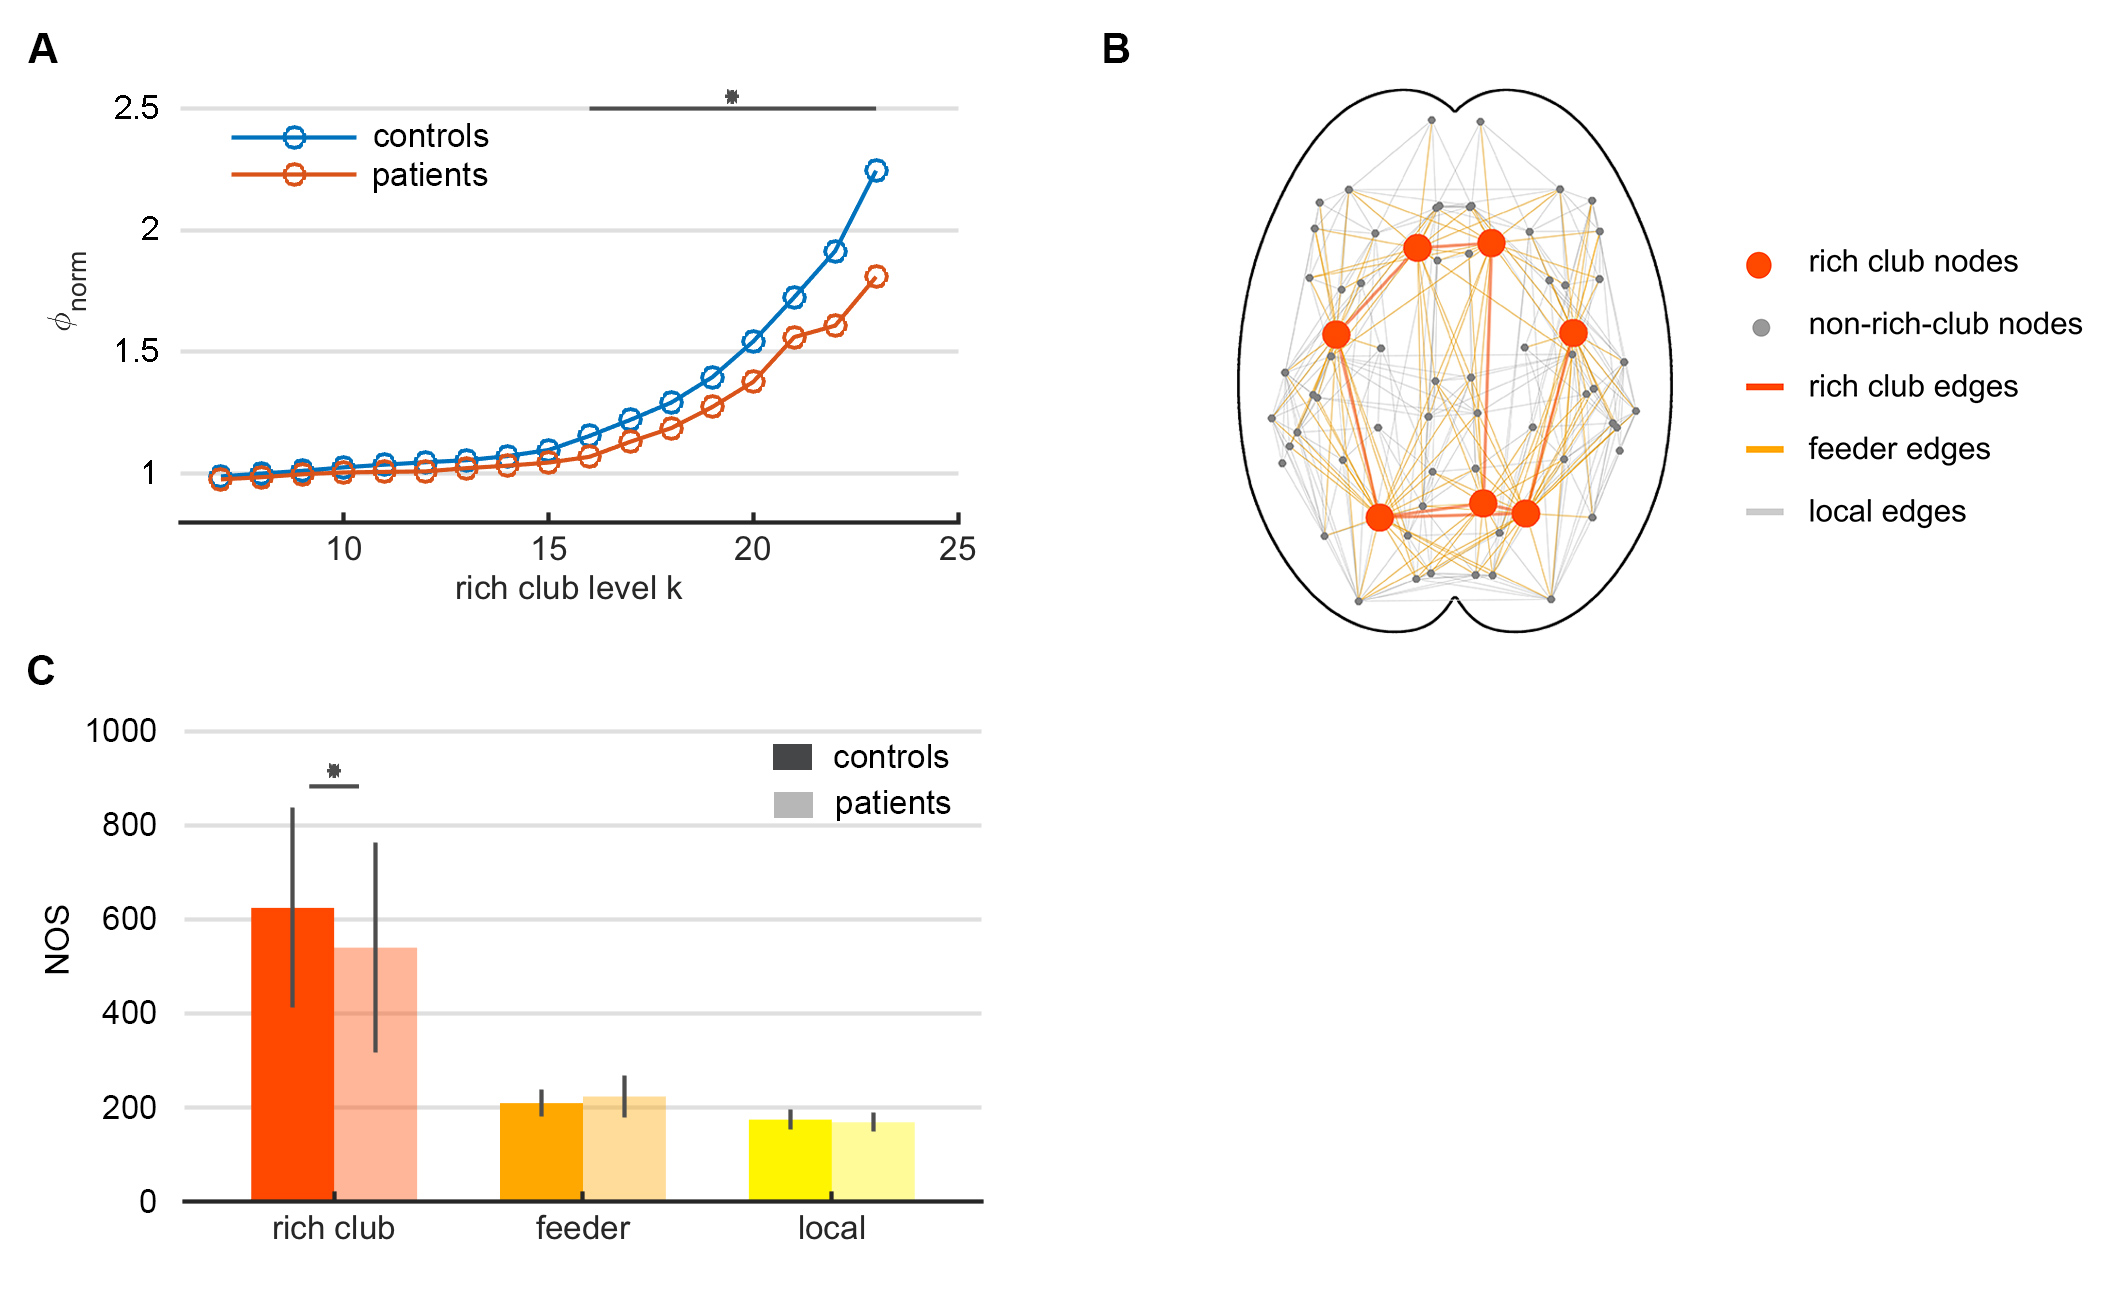
\includegraphics[width=\linewidth]{images/rcsczFig1.jpg}
  \caption{(A) Decreased rich club coefficient in patients (red) as compared with healthy controls (blue) for degree \textit{k} ranging from 16 to 23 (\pval = 0.012, 10,000 permutations, uncorrected). (B) Group-averaged structural network for healthy controls. Rich club regions (red) were identified by setting the threshold as degree > 18, including bilateral superior frontal gyri, superior parietal lobules, insula, and left precuneus. Connections were classified into 3 categories: rich club (red), feeder (orange), and local (gray) connections. (C) Group-averaged connectivity strength (number of streamlines [NOS] weighted) of the rich club (red), feeder (orange), and local (yellow) connections in healthy controls (dark) and patients (light). Error bars represent one standard deviation. Patients showed decreased rich club connection density in comparison with healthy controls (\pval = 0.032, 10,000 permutations, uncorrected).
}
  \label{rcsczFig1}
\end{figure}

\subsection*{SC-FC coupling}
Overall FC strength (average of the FC matrix) was found to be similar across patients and controls (\pval = 0.408, 10,000 permutations), as was the FC strength of rich club, feeder, and local connections (\pval > 0.526, 10,000 permutations). Both patients and healthy controls demonstrated a positive correlation between overall SC and FC values, with a mean (standard deviation) SC-FC correlation coefficient of 0.271 (0.064) for patients and 0.272 (0.060) for controls (Figure \ref{rcsczFig2}). SC-FC coupling was similar in patients compared to controls (\pval = 0.461, 10,000 permutations). Considering the distinct connection categories, a significantly reduced SC-FC coupling was detected for rich club connections in patients compared to controls (\pval < 0.001, 10,000 permutations, NOS-weighted), whereas no such difference in SC-FC coupling was found in feeder (\pval = 0.865) and local (\pval = 0.414) connections (Figure \ref{rcsczFig2}). Similar effects were found when correcting for age and gender (\pval < 0.001, 10,000 permutations) and when using SC networks weighted by SD (\pval < 0.001, 10,000 permutations).

\begin{figure}[h]
\centering
  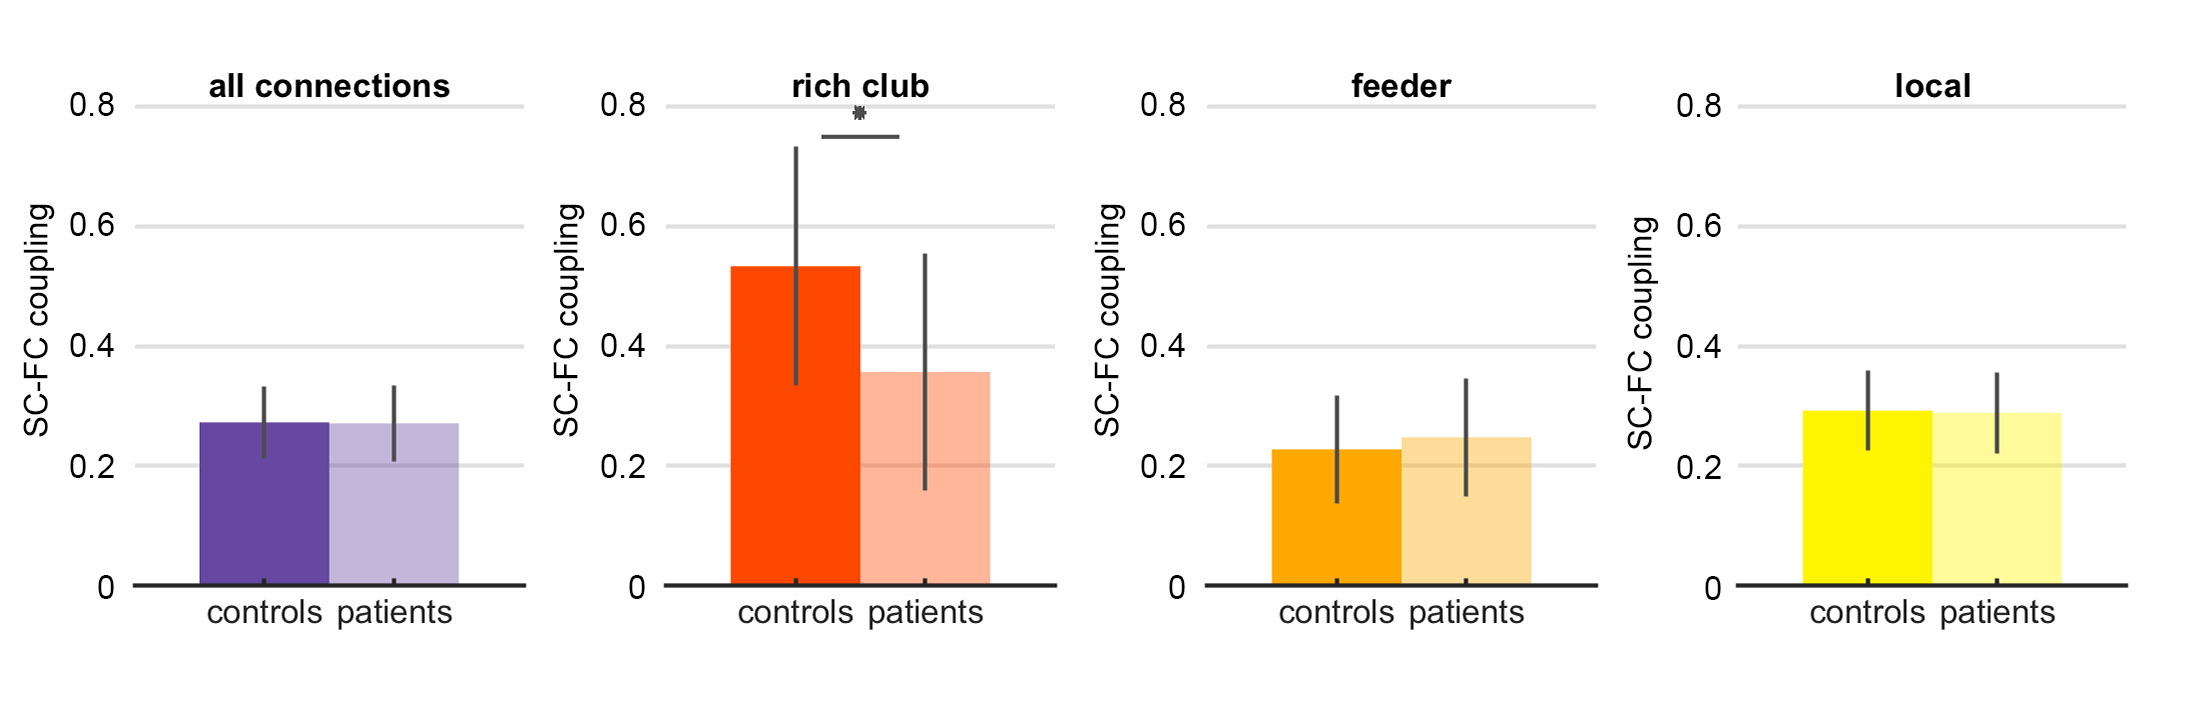
\includegraphics[width=\linewidth]{images/rcsczFig2.jpg}
  \caption{\small SC-FC coupling in healthy controls (dark) and patients (light) for all connections, rich club connections (\pval < 0.001, 10,000 permutations, false discovery ratio [FDR] corrected), feeder connections (no effect), and local connections (no effect). Error bars represent one standard deviation and asterisk indicates significance.}
  \label{rcsczFig2}
\end{figure}

\subsection*{Correlation between network organization and clinical Variables}
No specific association between rich club connections' strength and symptom scores was observed. In patients, the strength of feeder connections was found to be negatively correlated with PANSS positive score (NOS, \rval = -0.34, \pval = 0.030) and total score (\rval = -0.35, \pval = 0.022), suggesting that patients with weaker feeder connections may have more severe symptoms, especially with regard to positive symptoms. Strength of local connections was negatively correlated with PANSS positive score (NOS, \rval = -0.32, \pval = 0.043) and negative score (NOS, \rval = -0.36, \pval = 0.019) (Figure \ref{rcsczFig3}). No specific correlation was found for SD connectivity.

\begin{figure}[H]
\centering
  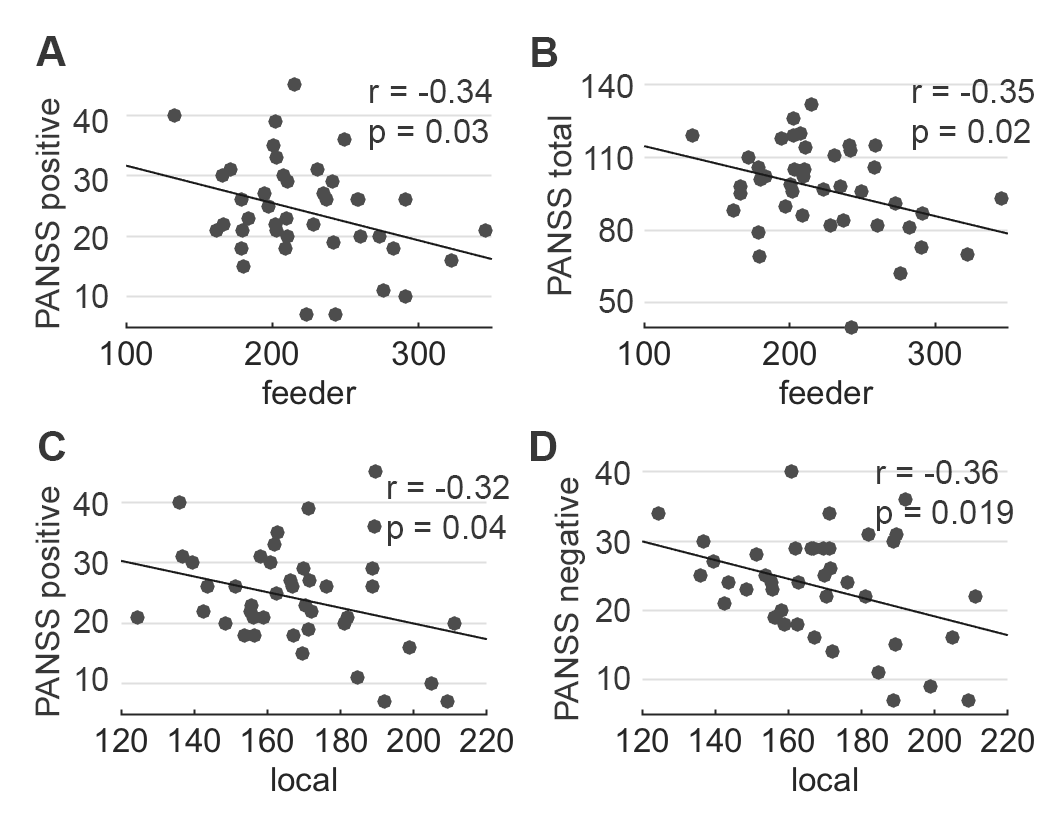
\includegraphics[width=8cm]{images/rcsczFig3.png}
  \caption{Feeder connections (NOS) were negatively correlated with (A) PANSS positive score (\rval = -0.34, \pval = 0.030, uncorrected) and (B) total score (\rval = -0.35, \pval = 0.022, uncorrected) in patients. Local connections (NOS) were negatively correlated with (C) PANSS positive score (\rval = -0.32, \pval = 0.043, uncorrected) and (D) negative score (\rval = -0.36, \pval = 0.019, uncorrected).}
  \label{rcsczFig3}
\end{figure}

\subsection*{Machine learning disease classification}
To explore the performance of classification using connectome measurements, we trained a quadratic support vector machine (SVM, see Supplementary Methods) based on structural connectivity strength and SC-FC coupling of rich club connections (see Supplementary Methods). Using five-fold cross-validation, we obtained a prediction accuracy of 73.3\% (sensitivity = 76\% and specificity = 71\%; Supplementary Figure \ref{figureS4:confusionmatrix}).

\subsection*{Replication dataset}
Patients' rich club effects were validated using the replication dataset. The cortical rich club was taken as the same set of regions as in the principal dataset (the two datasets showed high consistency in rich club organization, see supplementary results). Patients (10 medication-na\"{i}ve patients; results for the full replication dataset including 29 additional patients with a short medication history are shown in supplementary results) again showed a significant reduction in rich club connectivity strength compared with healthy controls (NOS, \pval = 0.021, 10,000 permutations), with no difference observed in feeder (\pval = 0.394) or local (\pval = 0.602) connections (Figure \ref{rcsczFig4}). Examining the SD of rich club connections showed similar results (rich club connectivity \pval = 0.015, 10,000 permutations). A marginal effect of reduced SC-FC coupling was observed for rich club connections (\pval = 0.048), with no effect for feeder (\pval = 0.713) and local (\pval = 0.921) connections.

\begin{figure}[h]
\centering
  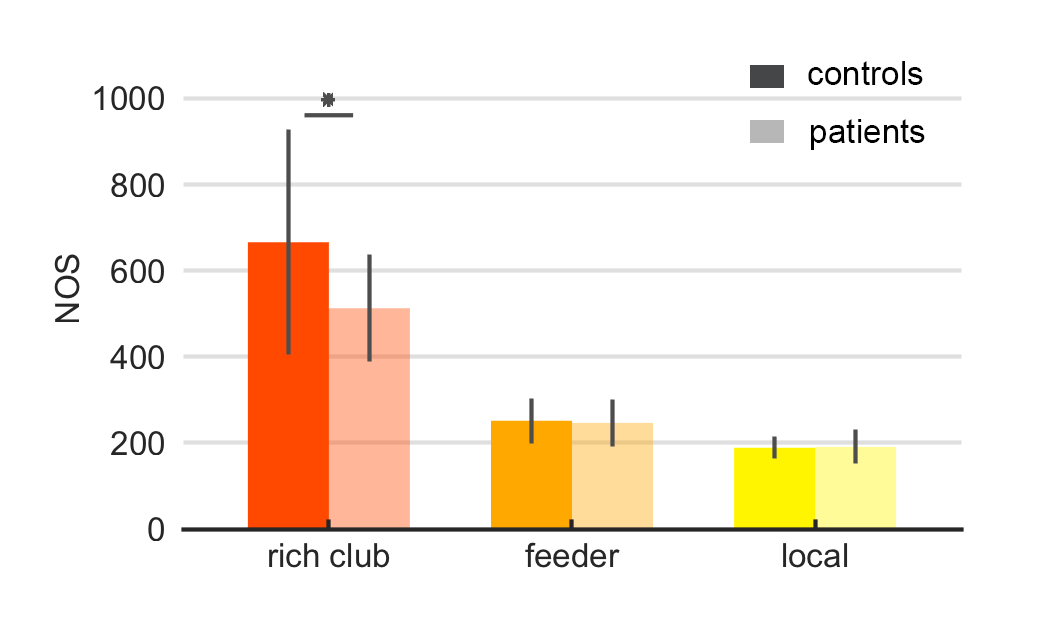
\includegraphics[width=8cm]{images/rcsczFig4.png}
  \caption{Replication dataset. Patients showed reduced rich club connection strength compared with healthy controls (NOS, \pval = 0.021, 10,000 permutations, uncorrected). No difference was observed in feeder (\pval = 0.394) and local connections (\pval = 0.602). Error bars represent one standard deviation and asterisk indicates significance.}
  \label{rcsczFig4}
\end{figure}


\section*{Discussion}
We investigated brain network organization in a sample of untreated, medication-na\"{i}ve first-episode schizophrenia patients. Rich club organization and structure-function coupling of rich club connections were found to be altered in patients compared to controls, suggesting that rich club organization may be already impaired in the early stages of schizophrenia.

Previous studies have noted the potential influence of medication on brain network findings in schizophrenia \citep{Crossley2017ConnectomicCO}. In the current study, we took extra care to rule out medical and therapeutic effects by examining first-episode, medication-na\"{i}ve patients. Our results suggest that the impairment of rich club organization directly relate to schizophrenia independently from possible confounding factors, advancing our understanding of the disease mechanisms during the early stages of the disorder.

Previous studies have reported aberrant rich club connectivity and functional brain dynamics in European chronic schizophrenia patients \citep{vanDenHeuvel2013AbnormalRC}. Similar findings have been reported in a cohort of North American chronic schizophrenia patients \citep{Yeo2016GraphMO} and, recently, in a large sample of Australian patients with schizophrenia or schizoaffective disorder \citep{Klauser2017WhiteMD}. Our study consolidates and extends these previous findings by showing an alteration of rich club organization in a cohort of Chinese patients and further underscores the cultural ubiquity of the biological underpinnings of schizophrenia.

Studies examining brain abnormalities in first-episode schizophrenia have reported fiber tract disruptions in the anterior limb of internal capsule \citep{Weiss2015ImprovedNA,Kelly2017WidespreadWM}, cingulum \citep{Xiao2018WhiteMA}, and anterior corona radiate \citep{Caprihan2015ThePR,Xi2016TheSC,Asmal2017InsightAW,Subramaniam2017WhiteMM}. The rich club regions identified in this study, i.e., the bilateral superior frontal gyri, superior parietal lobules, and insula, as well as the precuneus, are located in parts of the brain interconnected by the above-mentioned white matter tracts \citep{Greicius2008PersistentDN,vanDenHeuvel2009FunctionallyLR}. Rich club disruption is coherent with previous findings on schizophrenia patients \citep{vanDenHeuvel2013AbnormalRC,Collin2014ImpairedRC} and suggests that brain network alterations may be concentrated around the centrally connected areas of the human brain \citep{Klauser2017WhiteMD,Greicius2008PersistentDN,vanDenHeuvel2009FunctionallyLR}. In such highly connected fronto-parietal areas, myelination has been suggested to continue postnatally until the third decade of life \citep{Marn2016DevelopmentalTA,Silbereis2016TheCA}, which overlaps with the most frequent period of schizophrenia onset, occurring mostly in the early- to mid-20s for men and late-20s for women \citep{Abbas2013DIAGNOSTICAS}. Therefore, our observed structural rich club findings in first-episode patients may indirectly reflect an important neurodevelopmental feature of schizophrenia.

With converging evidence pointing to a rich club white matter impairment in both early and chronic stages of schizophrenia, a critical next step will be to determine and assess the potential value of these features in clinical applications. "Radiomics," defined as "the conversion of images to higher-dimensional data and the subsequent mining of these data for improved decision support," \citep{Gillies2016RadiomicsIA} represents the next step in promoting the translation \citep{Aerts2016ThePO} of brain connectome-based features to diagnosis and prediction for schizophrenia. A radiomics analysis involves the high-throughput extraction of meaningful measures (such as rich club connectivity) from medical images to support clinical decision processes \citep{Gillies2016RadiomicsIA}. Previous studies have suggested that gray matter abnormalities in schizophrenia are frequent, but quite heterogeneous across patients \citep{Wolfers2018MappingTH}, potentially limiting the contribution of gray matter features as a single biomarker for the disorder. Using machine learning techniques as a post-hoc analysis, we demonstrated the potential validity of individual rich club organizations (Supplementary Figure \ref{figureS3:scatter_scfc_nos}) for the classification of first-episode schizophrenia patients (see Supplementary Methods). Recent findings have shown that functional connectome organization may be an important source of information to predict the conversion to psychosis in a high-risk population \citep{Collin2018FunctionalCO}. Future studies combining multi-modal neuroimaging features may facilitate the identification of schizophrenia and further improve psychiatric care.

Several comments regarding the used methods and results need to be addressed. First, examining first-epi- sode schizophrenia patients, we obtained some distinct results compared to previous studies examining chronic schizophrenia \citep{vanDenHeuvel2013AbnormalRC,Yeo2016GraphMO,Klauser2017WhiteMD}. A decrease in SC-FC coupling was found in rich club connections in first-episode patients in our study, while an increase in SC-FC coupling in whole-brain connections has been observed in treated, chronic schizophrenia patients \citep{vanDenHeuvel2013AbnormalRC}. The heterogeneity of these findings could reflect the effects of medication and/or of the clinical history of the patients, but further investigation is warranted. Investigating the whole replication dataset (10 medication-na\"{i}ve and 29 treated patients) did not reveal alterations in rich club SC-FC coupling (\pval = 0.102 for NOS and 0.113 for SD). A second comment concerns the use of diffusion-weighted MRI and deterministic tractography to reconstruct cortico-cortical white matter pathways, as these methods are well-known to have several caveats regarding the reconstruction of complex oriented pathways \citep{Jbabdi2011TractographyWD}. We used a common clinical DWI protocol with a singleb-value of 1000 s/mm\textsuperscript{2}, which might be insufficient to resolve complex crossing fibers in the tractography \citep{Weiss2015ImprovedNA,Tournier2007RobustDO,Tournier2004DirectEO}. The use of higher magnetic field strength, higherb-value, more diffusion directions, and methods suitable for the reconstruction of complex fiber orientations (e.g., probabilistic tractography \citep{Behrens2007ProbabilisticDT} or constrained spherical deconvolution \citep{Tournier2007RobustDO,Tournier2004DirectEO}) may result in better reconstruction of white matter fiber pathways. Third, head movements during fMRI acquisition have been argued to be an important source of spurious signals in functional connectivity studies \citep{Power2012SpuriousBS,Yan2013ACA}. In this study, we performed scrubbing to reduce the effect of head motion, and including the head movement measures and number of scrubbed frames as covariates to the group-comparison statistical analyses revealed consistent findings (see supplementary results). Fourth, brain network architecture was characterized by means of graph theoretical metrics that have received large consensus in clinical connectome literature \citep{Fornito2012SchizophreniaNA,Heuvel2014BrainNI,Griffa2013StructuralCI,Fornito2015ConnectomicsAN}. Nevertheless, it has been noted that graph metrics can be highly correlated in real-world networks \citep{sporns_human_2005} and new network measures are continuously proposed \citep{Bertolero2017TheDC,Betzel2017MultiscaleBN}. Future research applying advanced network measures could bring further insights into the characteristics of brain network alterations in early schizophrenia and the clinical diagnosis.

This study shows a reduced level of structural rich club connectivity in first-episode schizophrenia patients with no or limited medication history. We suggest that connectome features including rich club impairment reflect pathophysiological processes occurring early in the course of schizophrenia, independently from the medication history of the patients. Our results are important for advancing our understanding of the neuropathological mechanisms of first-episode schizophrenia. They add important empirical support for the use of individual connectome organization as a potential marker for disease classification.
    
\section*{Funding}
This work was supported by the National Natural Science Foundation of China (grants 81801675 to L.-B.C., 81571651 to H.Y.); the State Scholarship Fund, China Scholarship Council (grants 201506040039 to Y.W., 201603170143 to L.-B.C); the Netherlands Organization for Scientific Research (grants ALWOP.179 and VIDI- 452-16-015 to M.P.vdH.); a fellowship of MQ (to M.P.vdH.); and the Swiss National Science Foundation (grant \#P2ELP3\_172087 to A.G.).

\section*{Acknowledgments}
We would like to acknowledge, with special thanks, Miss Xiao Chang at Department of Psychiatry, Brain Center Rudolf Magnus, University Medical Center Utrecht and Prof. Qingrong Tan and Prof. Huaning Wang at Department of Psychiatry, Xijing Hospital, Fourth Military Medical University for their help on this work.

\printbibliography[heading=subbibliography]

\end{refsection}

% SI
\begin{refsection}
\newpage
\section*{Supplementary Information}
\subsection*{Supplementary Methods}
\subsubsection*{Participants}
All subjects were right handed and their biological parents were of the Han Chinese ethnic group. Exclusion criteria for patients included: (1) presence of another psychiatric disorder; (2) history of receiving antipsychotics (or more than two weeks of antipsychotic medication for the replication dataset), history of repetitive transcranial magnetic or current stimulation, or a history of behavioral treatment; (3) history of clinically significant neurological, neurosurgical or medical illnesses; (4) substance abuse within the prior 30 days or substance dependence within the prior 6 months; (5) pregnancy or any other MR imaging contraindications, e.g., cardiac pacemakers and other metallic implants. Exclusion criteria for healthy controls included: (1) presence of any psychotic syndrome; (2) history of receiving antipsychotics, repetitive transcranial magnetic stimulation, transcranial current stimulation, or behavioral treatment; (3) history of clinically significant neurological, neurosurgical or medical illnesses; (4) substance abuse within the prior 30 days or substance dependence within the prior 6 months; (5) pregnancy or MR imaging contraindications, e.g., cardiac pacemakers and other metallic implants. In total, out a selected group of 113 patients and 124 controls, thirty-two patients and ten controls were excluded because of image quality and high head motion, resulting in the examined population of 81 patients and 114 controls. Dose of current antipsychotic drugs at time of MRI was converted using defined daily dose method (WHO Collaborating Centre for Drug Statistics Methodology, 2014) \citep{Leucht2016DoseEF}.

\subsubsection*{Data preprocessing}
\textit{T1-weighted images.} Cortical parcellation was obtained on the basis of T1-weighted images using the Freesurfer software (version 5.3.0). The automated recon-all pipeline was used, including segmentation of gray and white matter tissue, reconstruction of cortical mantle, and parcellation of the cortical mantle into 68 cortical areas. Cortical segmentations were checked manually for accuracy. 68 cortical regions (34 per hemisphere) were segmented according to the Desikan Killiany atlas \citep{DESIKAN2006968}. Two further subdivisions \citep{CAMMOUN2012386} (114 regions, 57 per hemisphere; and 219 regions, 108 in the right hemisphere and 111 in the left hemisphere) of the Desikan Killiany atlas were additionally used for validation purposes.

\textit{Diffusion weighted imaging (DWI).} Sixty-four DWI images (single-shell, b = 1000 s/mm$^{2}$) and a b = 0 image were realigned and corrected for small head movements and common gradient-induced distortions \citep{ANDERSSON2002177}. The diffusion profile within each voxel was reconstructed using generalized q-sampling imaging (GQI) \citep{YEH2010}. In addition, fractional anisotropy (FA) maps were computed from fitted single tensors \citep{Chang2005RESTORERE}. Deterministic tractography was performed to reconstruct white matter tracts, applying the Fiber Assignment by Continuous Tracking (FACT) algorithm \citep{Mori2002FiberTP}. For each white matter voxel, eight streamline seeds were started and tracking was stopped if the streamline reached a voxel of low fractional anisotropy (FA < 0.1), exited the gray matter/white matter mask, or made a sharp turn (> 45$^{\circ}$). All preprocessing steps were performed according to previous studies \citep{VANDENHEUVEL2016293,Romme2017ConnectomeDA}.

\textit{Resting-state functional magnetic resonance imaging (rs-fMRI).} Resting-state fMRI data of each subject were realigned and co-registered with the T1-weighted image to overlap with the resultant cortical parcellation maps. Second, the blood oxygenation level-dependent (BOLD) time series were corrected for linear trends, as well as global nuisance covariance, including 6 head motion parameters and mean signals of white matter and ventricles. Third, band-pass filtering (0.01-0.1 Hz) was performed together with motion scrubbing to minimize the influence of head-motion \citep{Power2012SpuriousBS}. Each slice with framewise displacement (FD) exceeding 0.25 (defined as the sum of the absolute derivatives of the six realignment parameters) and dynamic variability (DVARS) exceeding 1.5, as well as 1 back neighbour, were removed following the procedure by Power et al. \citep{Power2012SpuriousBS}.

\subsubsection*{Graph metrics}
\textit{Connectivity strength.} Connectivity strength (\textit{S}) was computed as the average weight of all connections within the network as follows:
\[\mathsf{S=\overline{W}}\]
where \textit{W} indicates connectivity weights of the reconstructed network edges.\\

\noindent
\textit{Network density.} Network density (\textit{D}) was computed by dividing the number of connections existed in the network by the number of connections in the fully-connected network as follows:
\[\mathsf{D=\frac{E}{n(n-1)/2}}\]
with \textit{E}, the number of connections and \textit{n}, the number of nodes.\\

\noindent
\textit{Clustering coefficient.} Clustering coefficient, \textit{Ci}, reflects the level of local connectedness of a node, and was computed by dividing the geometric mean of triangles around a node by the maximum number of possible triangle around a node. The global level of clustering coefficient was obtained by averaging the clustering coefficient of all nodes within the network as follows:
\[\mathsf{C=\frac{1}{n}\sum_{i \in N} \frac{\sum_{j,h \in N} (w_{ij}w_{ih}w_{jh})^{1/3}}{k_{i}(k_{i}-1)}}\]
where \textit{N} the set of all nodes and $\mathsf{k_{i}}$ the degree of node \textit{i} (i.e., the number of connections linked to node \textit{i}). Normalized clustering coefficient \textgamma, was obtained by comparing the clustering coefficient in brain network to those in 1000 random networks as follows:
\[\mathsf{\gamma=\frac{C}{\overline{C_{random}}}} \]   \\

\noindent
\textit{Shortest path length.} The shortest path (\textit{d}) between two nodes was taken as the minimum edges' weights needed to traverse from one node to the other \citep{RUBINOV20101059}. The mean shortest path length of a network (\textit{L}) was taken as the average shortest path length between all pairs of nodes in the network as follows:
\[\mathsf{L=\frac{1}{n} \sum_{i \in N} {\frac{\sum_{j \in N,j \neq i} {d_{ij}}}{n-1}}}\]
Normalized path length \textlambda \ was computed by dividing the mean shortest path length in brain network by those in 1000 random networks as follows:
\[\mathsf{\lambda=\frac{L}{\overline{L_{random}}} }\] \\

\noindent
\textit{Rich club.} Weighted rich club coefficient $\mathsf{\Phi_{w}(k)}$ was assessed \citep{Opsahl2008ProminenceAC}. First, all connections of the network (weighted by streamline count) were ranked according to their weight, resulting in a vector $\mathsf{W^{ranked}}$. Second, sub-networks containing nodes with a degree larger than \textit{k} (where degree is the number of binary connections linked to each node) were selected for \textit{k} ranging from 5 to 40. Third, the number of edges within the selected sub-network ($\mathsf{E_{>k}}$) was determined and the sum of their weights ($\mathsf{W_{>k}}$) was computed. Fourth, the strongest $\mathsf{E_{>k}}$ edges of the whole network were selected and summed up, as computed by summing the top $\mathsf{E_{>k}}$ edges' weights in the ranked weights $\mathsf{W^{ranked}}$. Finally, the weighted rich club parameter $\mathsf{\Phi_{w}(k)}$ was computed as the ratio between $\mathsf{W_{>k}}$ and the sum of the strongest number of links $\mathsf{E_{>k}}$ in the total network by the following:
\[\mathsf{\Phi^{w}(k)=\frac{W_(>k)}{\sum_{l=1}^{E_{>k}} w^{ranked}_{l}}}\]
The weighted rich club parameter $\mathsf{\Phi_{w}(k)}$ was normalized by comparing to 1,000 random networks, to determine to what extent the observed connection strength between rich club nodes exceeds that predicted by the random null model, driven by node degree alone. Normalized rich club coefficient $\mathsf{\Phi_{norm}(k)}$ was computed as the ratio of $\mathsf{\Phi_{w}(k)}$ in the brain network to the mean of $\mathsf{\Phi_{random}(k)}$ across random networks, 
\[\mathsf{\Phi_{norm}(k)=\frac{\Phi(k)}{\Phi_{random}(k)} }\]
with a normalized rich club coefficient $\mathsf{\Phi_{norm}(k)}$ > 1 expressing the presence of a rich club organization in the network. Random networks were generated by shuffling edges in the structural network, preserving connection weights and the (binary) degree distribution \citep{Maslov2002SpecificityAS}. The rich club coefficient was computed until less than three nodes could be included in the examined set. Graph metrics and null models were computed using the MATLAB-based Brain Connectivity Toolbox \citep{RUBINOV20101059}.

\subsubsection*{Rich club nodes}
Rich club nodes were defined by selecting the nodes with degree \textit{k} \ > 18 in the group-averaged structural network of all subjects, resulting in 7 hub nodes (top 10\% percent high degree nodes in the network). Alternatively, we selected rich club nodes on the basis of individual structural networks of all subjects by setting the rich club threshold as degree > 18 and choosing the top 10\% mostly consistent rich nodes across subjects. A similar set of nodes was identified, including bilateral superior parietal lobe, superior frontal lobe, precuneus, and right insula. Furthermore, we also used a range of degree levels (\textit{k} \ > 14 - 22) as thresholds to define rich club nodes and observed similar findings (Supplementary Results). Results were thus consistent across different types of rich club selection.

\subsubsection*{Machine learning classification analysis}
Taking the principle dataset, a machine learning quadratic support vector machine (SVM) was fitted to the data of connectivity weights (NOS) and SC-FC coupling of rich club connections, as well as other demographic features, such as age, gender, and education time. Validation analysis was performed using 5-fold cross-validation (i.e., data samples were divided into 5 sub-datasets, with 4 sub-datasets taken as the training datasets and the other as the validation dataset, iterating for 5 times). Accuracy was calculated for the fitted model as the proportion of true predictions among the total number of cases. Sensitivity and specificity were computed as the proportions of actual positives and actual negatives that were correctly identified, respectively. Training was performed using the Classification Learner App embedded in MATLAB R2018a.

\subsection*{Supplementary Results}
\subsubsection*{Validation dataset}
\textit{Graph metrics.} The replication dataset used in the main text (i.e., only 10 untreated patients included) demonstrated no group difference for the network density (\pval = 0.428), connectivity strength (\pval = 0.622), clustering coefficient (\pval = 0.992), normalized clustering \textgamma, \pval = 0.819), and shortest path length (\pval = 0.135). Patients showed a slight increase in normalized shortest path length \textlambda \ compared to controls (\pval = 0.019).\\

\noindent
\textit{Using the whole dataset.} Here we reported results obtained by including 39 first-episode schizophrenia patients (10 untreated, medication na\"{i}ve patients and 29 patients with no more than two weeks of cumulative exposure to antipsychotics). Similar as in the discovery principal dataset, no difference was observed for network density (\pval = 0.171), connectivity strength (\pval = 0.073), and clustering coefficient (\pval = 0.554; for normalized \textgamma, \pval = 0.491). A slight reduction in shortest path length (\pval = 0.018; for normalized \textlambda, \pval = 0.008) in patients as compared to controls was observed.

With respect to the rich club structure, patients showed a significant reduction in rich club connection strength compared with healthy controls (NOS, \pval = 0.025, 10,000 permutations), with no difference observed in feeder (\pval = 0.117) and local connections (\pval = 0.137). Examining the streamline density of rich club connections showed a non-significant attenuated effect (\pval = 0.083, 10,000 permutations). Considering the slight age bias in replication dataset (\pval = 0.086), we excluded the six oldest subjects from control group (\pval = 0.403 after exclusion) to examine the potential effect of age on our results. Analyses on the remaining subjects showed significant rich club connection disruptions in patients for the predefined rich club regions (\pval = 0.026, NOS weights). No difference of SC-FC coupling was observed in patients for rich club (\pval = 0.247), feeder (\pval = 0.808), local (\pval = 0.800) and overall (\pval = 0.807) connections. Significant SC-FC coupling reductions was observed for rich club connections with intermediate-to-long fiber distances (> 50 mm, \pval = 0.028). \\

\noindent
\textit{Rich club regions in the replication dataset.} Rich club regions selected in the principal dataset belonged to the top 11 highest degree regions observed in the replication dataset, indicating high consistency in rich club organization across the two datasets. To further verify our findings, we examined rich club nodes based on the replication dataset by choosing nodes with degree > 20 (10 nodes) in the group structural network. The selected rich club nodes included bilateral precuneus, insula, rostral middle frontal cortex, superior frontal cortex and superior parietal cortex. The effect of disruptions in the rich club connection in patients was significant (\pval = 0.035, NOS weights). SC-FC coupling for rich club, feeder, and local connections did not show differences in patients as compared to controls (\pval = 0.549, 0.960, and 0.537, separately)

\subsubsection{Comparison between schizophrenia patients from the two datasets}
To verify that patients from both cohorts were neurobiologically similar, we additionally compared the rich club organization between the two untreated first-episode schizophrenia groups used in the main results. We found that the mean NOS within the entire brain only showed a trend-level difference between the two groups of patients (\pval = 0.051, 10,000 permutations). Specifically, no difference was observed for the rich club (\pval = 0.752, 10,000 permutations) and feeder (\pval = 0.164, 10,000 permutations) connections, with only significant difference for the local connections (\pval = 0.016, 10,000 permutations). Moreover, no difference was found for the SC-FC coupling of the rich club (\pval = 0.098, 10,000 permutations), feeder (\pval = 0.239, 10,000 permutations), and local (\pval = 0.259, 10,000 permutations) connections. These findings indicated that rich club organization and functional dynamics of patients from the two cohorts were similar.

\subsubsection*{Validation of brain parcellations}
Considering the influence of different node definitions on graph properties \citep{Fornito2010NetworkSE}, findings were verified by using two finer subdivisions of the Desikan-Killiany atlas [114 regions (DK-114) and 219 regions (DK-219)] \citep{CAMMOUN2012386}. 14 out of 114 regions (12.8\%) and 21 out of 219 regions (9.6\%) were taken as rich club regions, separately. For both atlases (Supplementary Figure \ref{figureS1:dk114and250}), patients consistently showed reduced streamline volume density of rich club connections (DK-114: \pval = 0.035 and DK-219: \pval < 0.001, 10,000 permutations) in contrast to controls, while no difference was found for feeder and local connections (DK-114: \pval = 0.343 and 0.561, for feeder and local connections; DK-219: \pval = 0.261 and 0.886, for feeder and local connections, 10,000 permutations; Supplementary Figure \ref{figureS1:dk114and250}). The SC-FC coupling for rich club connections was decreased in patients (\pval = 0.008 and 0.003, separately for the two parcellations, 10,000 permutations) (Supplementary Figure \ref{figureS1:dk114and250}). Local connection weights showed negative correlation with the PANSS negative scores (\rval = -0.33 and -0.32, \pval = 0.030 and 0.054, separately) and PANSS total scores (\rval = -0.35 and -0.37, \pval = 0.021 and 0.016, separately). These findings suggest that the definition of nodes and the network size didn't affect the reported rich club changes in first-episode patients.

\subsubsection*{Validation of fiber reconstruction strategy}
In the main analysis, GQI \citep{YEH2010} was used to reconstruct the diffusion signal of voxels within the DWI data. Alternatively, we fitted the diffusion profile of each voxel to a simple tensor using a robust tensor fit method based on an M-estimator \citep{Chang2005RESTORERE} and examined our main results. Both patients and controls consistently showed a rich club structure, with a significantly decreased rich club coefficient in patients as compared with controls (\pval = 0.040, for rich club of k ranging from 16 to 23, 10,000 permutations). Furthermore, we observed a significant decrease in rich club connections (\pval = 0.047, NOS weights, and \pval = 0.023, SD weights, 10,000 permutations) and rich club SC-FC couplings (\pval = 0.001, NOS weights, and \pval = 0.003, SD weights, 10,000 permutations) in patients. Correlation analysis showed that rich club connection weights were positively correlated to the PANSS supplementary score (P4, P7, G6, S1, S2, and S3) (\rval = 0.31, \pval = 0.047). Feeder connection weights were negatively correlated to PANSS positive score (\rval = -0.35, \pval = 0.022) and total score (\pval = -0.34, \pval = 0.027). Local connection weights were also negatively correlated to PANSS negative score (\rval = -0.41, \pval = 0.006) and total score (\pval = -0.28, \pval = 0.031).

\subsubsection*{Validation of global signal correction in resting-state fMRI data}
We also evaluated the structural connectivity-functional connectivity (SC-FC) coupling alterations in patients after correcting the global signal during fMRI data preprocessing \citep{Murphy2017TowardsAC}. Patients reliably showed decreased SC-FC coupling level for rich club connections (\pval = 0.001, 10,000 permutations) compared with controls in the principle dataset, suggesting that global signal correction did not change the nature of the reported results.

\subsubsection*{FA weights}
Connections were also weighted by FA to reflect microstructure properties of white matter \citep{Beaulieu2002TheBO}. The FA-weighted structural networks in patients showed no difference in connection strength (\pval = 0.234), clustering coefficient (\pval = 0.852) or mean shortest path length (\pval = 0.344), and normalized shortest path length (\pval = 0.664). A decreased normalized clustering coefficient was observed in patients (\pval = 0.023, not corrected). The rich club coefficient showed no significant difference between the two groups (\pval > 0.112). Connection weights (i.e., mean FA) and SC-FC coupling for all three categories of connections also showed no difference between groups (\pval = 0.600, 0.887, and 0.836, for weights of rich club, feeder, and local connections, respectively; \pval = 0.766, 0.831, and 0.379, for SC-FC coupling of rich club, feeder, and local connections, respectively; 10,000 permutations).

\subsubsection*{Validation of rich club levels}
Rich club regions in the main analysis were selected by setting a rich club level of k > 18 (top 10\% high degree nodes) in the group-averaged structural network. We also performed our main analysis on the basis of a range of rich club level k from 14 (top 28\% high degree nodes) to 22 (top 3\% high degree nodes). For each k level, the average rich club connection weights (SD-weighted) are illustrated in (Supplementary Figure \ref{figureS2:range}). Rich club connection density was significantly reduced in patients as compared with controls in the range of k from 18 to 22 (\pval  < 0.05, 10,000 permutations), corresponding to 13\% to 3\% highest degree nodes included into the rich club. SC-FC coupling of rich club connections was significantly reduced in patients compared with controls in the range of \textit{k} from 14 to 20 (\pval < 0.05, 10,000 permutations) (Supplementary Figure \ref{figureS2:range}).

\subsubsection{Assessment of head motion in resting-state fMRI data}
We assessed the potential effect of head movements in the fMRI datasets. Comparing the mean FD between patients and controls showed no significant difference in both the principle dataset (\pval = 0.303) and the replication dataset (\pval = 0.103; 10,000 permutations). In the principle dataset, patients showed a larger number of scrubbed volumes compared to the controls (\pval = 0.042), but this effect was not observed in replication dataset (\pval = 0.409, 10,000 permutations). Furthermore, examining the SC-FC coupling differences between patients and controls with the mean FD and number of scrubbed volumes included as covariates showed similar results as reported in the main analysis (rich club connections: \pval < 0.001 in principle dataset and \pval = 0.024 in replication dataset; 10,000 permutations), suggestive of our results not to be driven by the effects of head motion.

\subsection*{Supplementary References}
\printbibliography[heading=none]

\newpage
\subsection*{Supplementary Tables}

\scriptsize
\captionof{table}{Detailed Scanning Parameters} \label{tableS1:MRI} 
\resizebox{\textwidth}{!}{\begin{tabular}{@{}llllclllclll@{}}\toprule
& \multicolumn{3}{c}{Siemens scanner} & \phantom{abc}& \multicolumn{3}{c}{GE scanner} \\
\cmidrule{2-4} \cmidrule{6-8}
& T1 & DWI & fMRI && T1 & DWI & fMRI \\
\midrule
TR (ms) & 2530 & 2000 & 7000 && 8.2 & 2000 & 10000 \\
TE (ms) & 3.5 & 30 & 91 && 3.2 & 30 & 82.4 \\
Flip angle ($^{\circ}$) & 7 & 90 & NA && 12 & 90 & NA \\
FOV (mm\textsuperscript{2}) & 256 × 256 & 220 × 220 & 256 × 256 && 256 × 256 & 240 × 240 & 240 × 240 \\
Matrix & 256 × 256 & 64 × 64 & 128 × 128 && 256 × 256 & 64 × 64 & 128 × 128 \\
Slice thickness (mm) & 1 & 4 & 3 && 1 & 3.5 & 2 \\
Section gap (mm) & 0 & 0.6 & 0 && 0 & 0 & 0 \\
Number of slices & 192 & 33 & 50 && 196 & 45 & 70 \\
\bottomrule
\end{tabular}}
\bigskip
\scriptsize Abbreviations: FOV, field of view; NA, not applicable; TE, echo time; TR, repetition time (ms).

\bigskip

\scriptsize
\centering
\captionof{table}{Correlations between the number of streamlines (NOS) and PANSS scores}
\label{tableS2:Corr} 
\begin{tabular}{llllll}\toprule
 &Positive&Negative&General&Supplementary&Total\\
 \midrule
NOSrc&-0.059&0.280&0.103&0.194&0.138\\
NOSfeeder&-0.335*&-0.243&-0.213&-0.023&-0.353*\\
NOSlocal&-0.316*&-0.362*&-0.016&-0.064&-0.297\\
\bottomrule
\scriptsize *  \textit{p} < 0.05, uncorrected
\end{tabular}

\bigskip

\newpage
\begin{flushleft}
\subsection*{Supplementary Figures}
\end{flushleft}

\begin{figure}[H]
\centering
  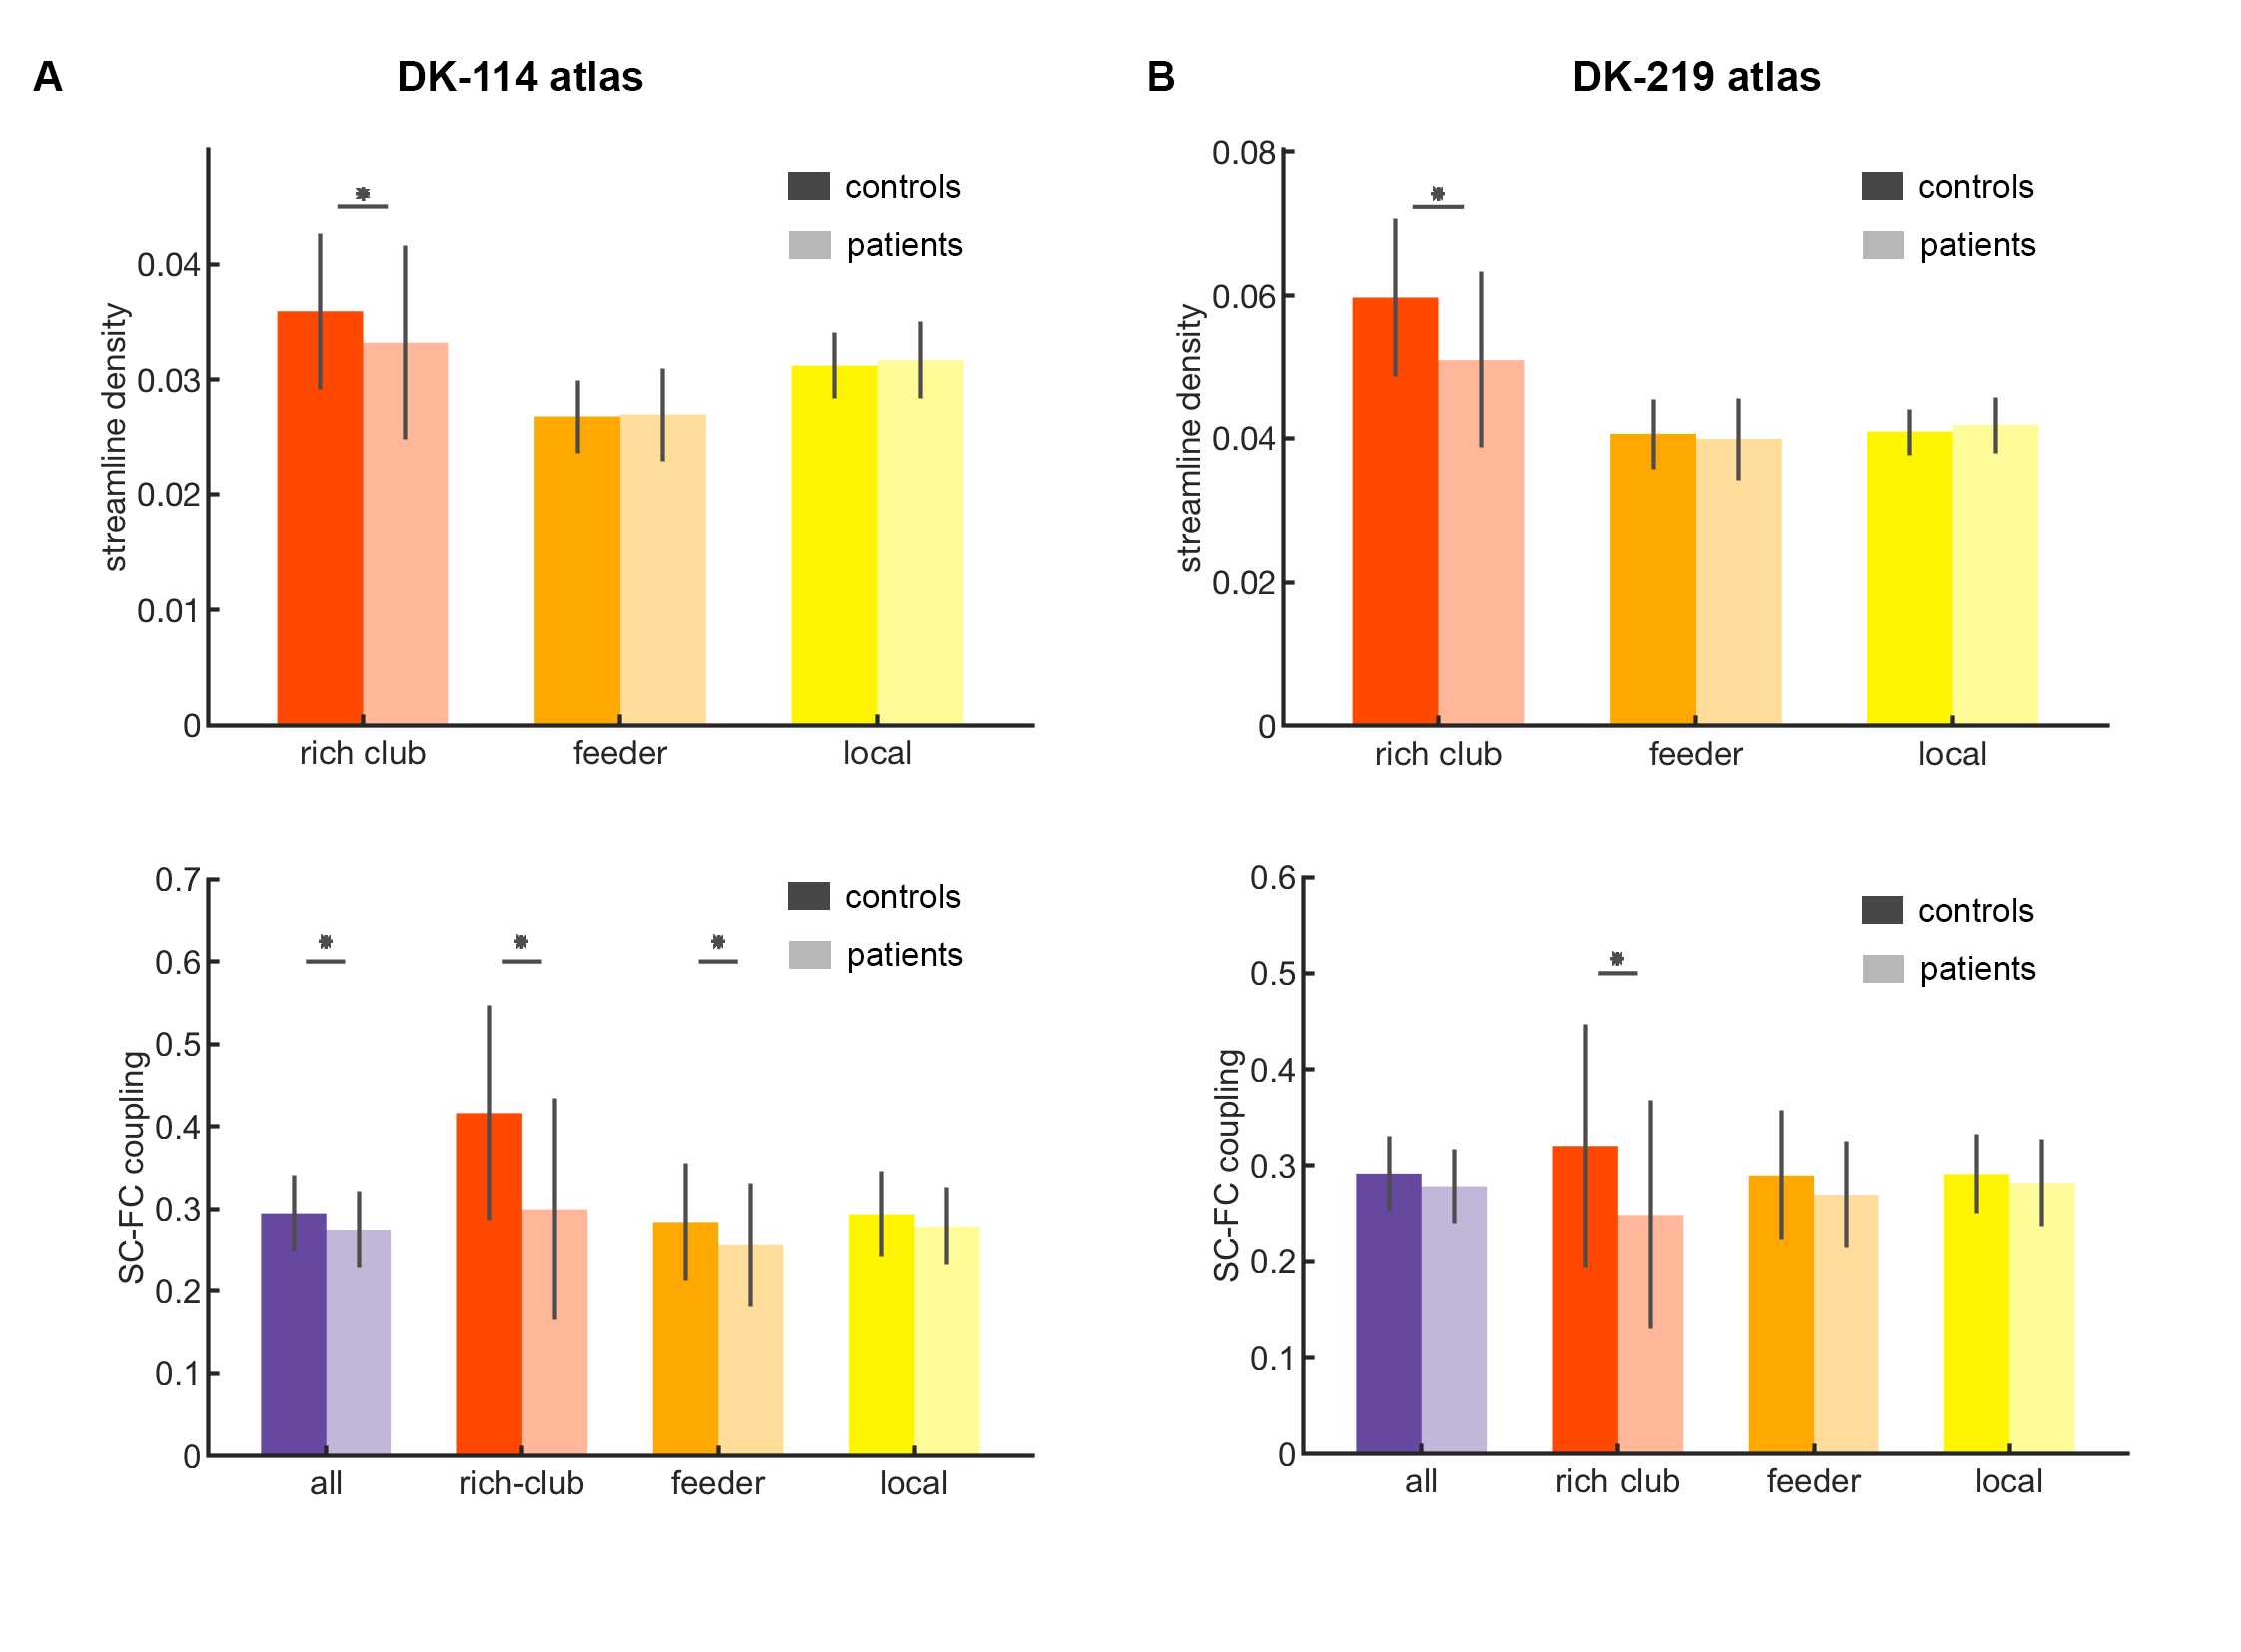
\includegraphics[width=\linewidth]{images/rcsczFigS1.png}
  \caption{\small Results using two finer subdivisions of Desikan-Killiany atlas. (A) DK-114 atlas. Top: patients showed reduced streamline volume density of rich club connections (\pval = 0.035), but not for feeder (\pval = 0.343) and local connections (\pval = 0.561). Bottom: patients showed reduced SC-FC coupling of overall (\pval = 0.023), rich club (\pval < 0.001), and feeder connections (\pval = 0.034), but not for local connections (\pval = 0.087). (B) DK-219 atlas. Top: patients showed reduced streamline volume density of rich club connections (\pval < 0.001), but not for feeder (\pval = 0.261) and local connections (\pval = 0.886). Bottom: patients showed reduced SC-FC coupling of rich club connections(\pval = 0.003), but not for overall (\pval = 0.060), feeder connections (\pval = 0.064), and local connections (\pval = 0.150).).
}
  \label{figureS1:dk114and250}
\end{figure}

\begin{figure}[H]
\centering
  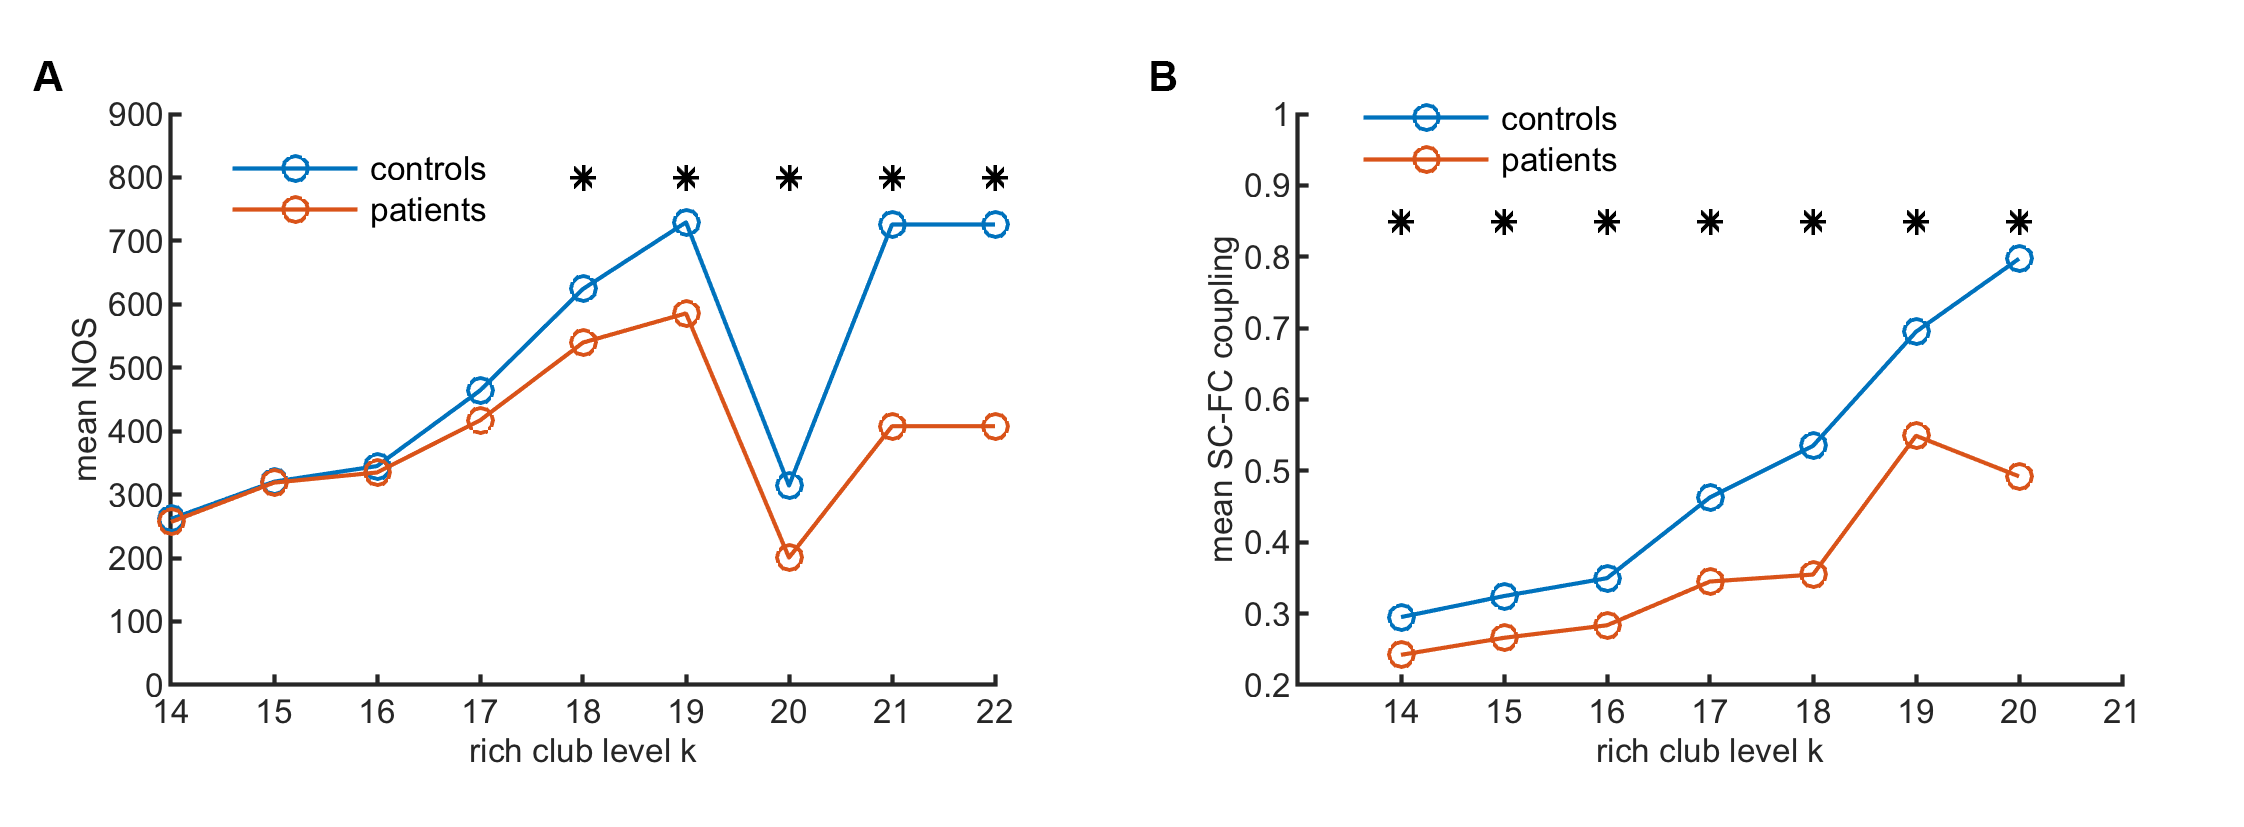
\includegraphics[width=\linewidth]{images/rcsczFigS2.png}
  \caption{\small Rich club alterations in distinct rich club levels. (A) The mean NOS of rich club connections at distinct rich club levels. Patients showed decreased rich club connection weights at k ranged from 18 to 22. (B) The mean SC-FC coupling of rich club connections at distinct rich club levels. Patients showed decreased SC-FC coupling at k ranged from 14 to 20. * indicates effects of \pval < 0.05.
}
  \label{figureS2:range}
\end{figure}

\begin{figure}[H]
\centering
  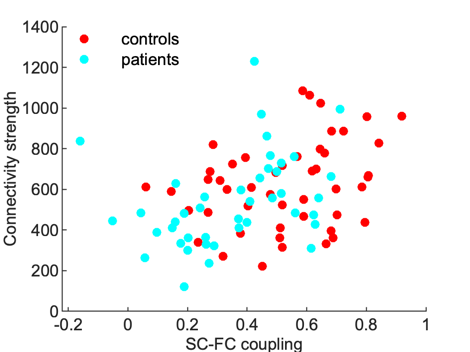
\includegraphics[width=7cm]{images/rcsczFigS3.png}
  \caption{\small Scatter plot of individuals' rich club measurements (in principle dataset). X axis describes SC-FC coupling of rich club connections and Y axis denotes connectivity strength (NOS) of rich club connections.
}
  \label{figureS3:scatter_scfc_nos}
\end{figure}

\begin{figure}[H]
\centering
  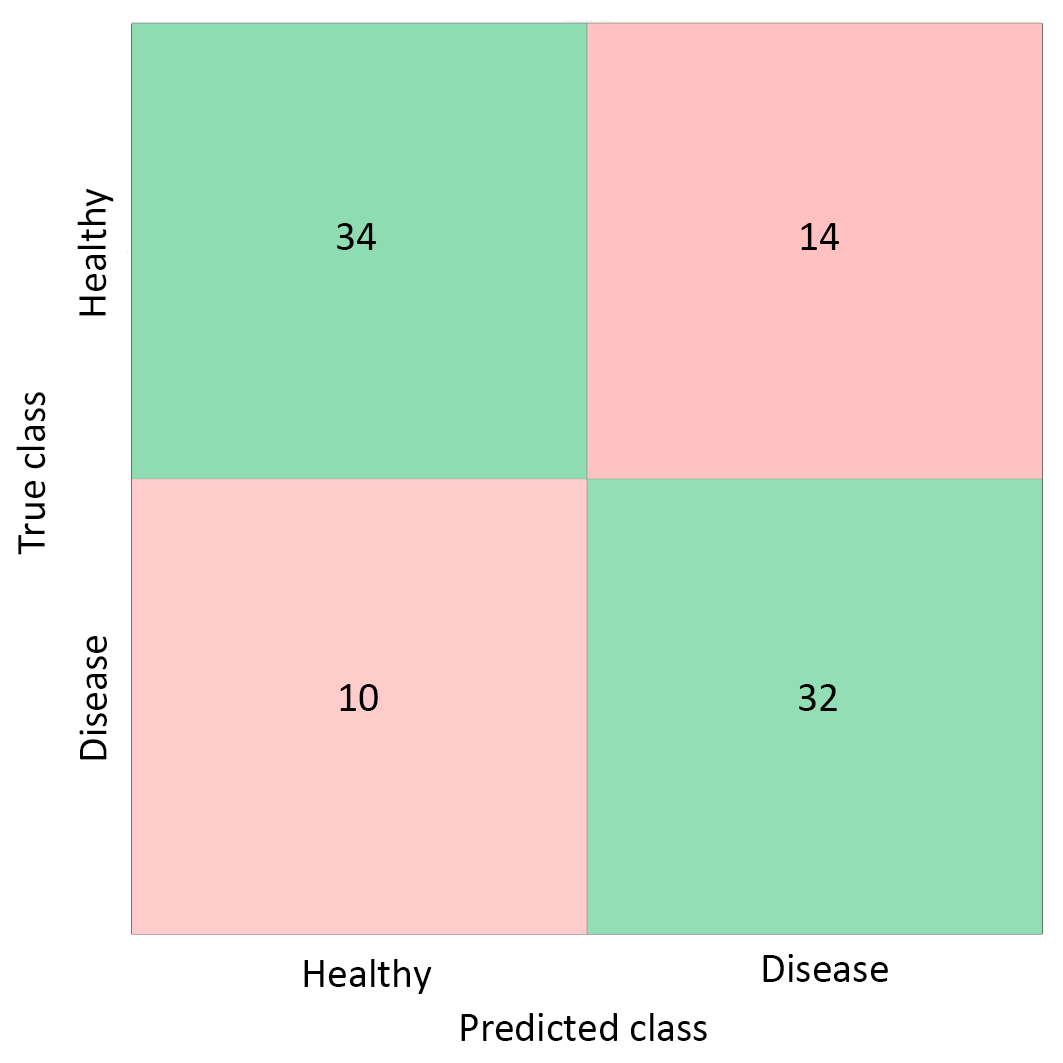
\includegraphics[width=7cm]{images/rcsczFigS4.png}
  \caption{\small Confusion matrix for the machine learning classification. Rows show the true class, and columns show the predicted class. The number of samples in each class are displayed. Green indicates that the true class and predicted class match, otherwise red.
}
\label{figureS4:confusionmatrix}
\end{figure}


\end{refsection}



% \chapter[MTR abnormalities and dysconnectivity in schizophrenia]{Cortical magnetization transfer abnormalities and connectome dysconnectivity in\\ schizophrenia}
\label{ch:mtrscz}

\begin{flushright}
\textit{Yongbin Wei, Guusje Collin, René C.W. Mandl, Wiepke Cahn, Kristin Keunen, \\Ruben Schmidt, René S. Kahn, Martijn P. van den Heuvel,
}\\
Schizophrenia Research, 2018; 192: 172-178
\vspace{7 mm}

\end{flushright}

\begin{refsection}
\newpage
\section*{Abstract}
Macroscale dysconnectivity in schizophrenia is associated with neuropathological abnormalities. The extent to which alterations in cortical myelination as revealed in vivo by magnetization transfer ratio (MTR) are related to macroscale dysconnectivity remains unknown. We acquired magnetization transfer imaging (MTI) data and diffusion weighted imaging (DWI) data from 78 schizophrenia patients and 93 healthy controls for MTR extraction and connectome reconstruction to examine the possible link between cortical myelination and macroscale dysconnectivity. Our findings showed significant cortical MTR disruptions in several prefrontal areas in schizophrenia patients, including bilateral rostral middle frontal areas, right pars orbitalis, and right frontal pole. Furthermore, cortical MTR alterations between patients and controls were significantly correlated with the level of regional disconnectivity. Together, our findings provide evidence that microstructural neuropathological abnormalities in schizophrenia are predominately present in prefrontal areas of the cortex and are associated with alterations in structural connectome architecture at the whole brain network level.

\section*{Introduction}
Schizophrenia is a severe psychiatric disorder that is characterized as a disorder of brain connectivity \citep{Fornito2012SchizophreniaNA,Stephan2009DysconnectionIS,Heuvel2014BrainNI}. In the past two decades, empirical magnetic resonance imaging (MRI) studies have provided a large body of evidence for disruptions of interregional connectivity \citep{EllisonWright2009MetaanalysisOD,Fornito2012SchizophreniaNA,Klauser2017WhiteMD,Fitzsimmons2013ReviewOF}. Connectome studies focused on brain network topology offer further support for this hypothesis by presenting converging evidence of decreased network efficiency \citep{Zalesky2011DisruptedAF}, less centralized frontal and parietal hubs \citep{vanDenHeuvel2010AberrantFA}, and reduced rich club organization in schizophrenia \citep{Collin2014ImpairedRC,vanDenHeuvel2013AbnormalRC}.

In terms of microscale neuropathology in schizophrenia, a wide range of histological alterations have been observed in the cerebral cortex (for a review, see \citep{Bakhshi2015TheNO}). Findings include increased neuronal density \citep{DorphPetersen2009PyramidalNN,Selemon1995AbnormallyHN,Selemon1998ElevatedND,Yang2011IncreasedIW}, decreased neuron size \citep{Chana2003TwodimensionalAO,Rajkowska1998NeuronalAG}, reduced dendritic spines density \citep{Garey1998ReducedDS,Glantz2000DecreasedDS,Glausier2013DendriticSP,Penzes2011DendriticSP} and reduced oligodendroglia density \citep{Uranova2004OligodendroglialDI,Uranova2001ElectronMO,Vostrikov2013ReducedOD}. Alterations in neuronal, synaptic and dendritic density have been suggested to underlie gray matter changes as revealed by neuroimaging studies \citep{Fornito2009AnatomicalAO,Fornito2009ReconcilingNA} and oligodendrocyte and myelination dysfunction have been linked to perturbations of white matter connectivity in schizophrenia \citep{Cassoli2015DisturbedMI}. In a recent study, we confirmed the pattern of abnormalities in spine density of pyramidal neurons across the cortex to be associated with the pattern of white matter connectivity changes in schizophrenia \citep{VANDENHEUVEL2016293}.

Magnetization transfer ratio (MTR) obtained by means of magnetization transfer imaging (MTI) provides an estimate of in vivo brain microstructure, in particular myelination levels \citep{Whitaker2016AdolescenceIA}, a technique that could complement post-mortem investigations of neuronal structure. MTR detects subtle changes in protons that are tightly bound to macromolecular structures, such as myelin, cell membrane proteins, and phospholipids \citep{wolff1994magnetization}. Indeed, MTR reductions in white matter have been shown to be associated with myelin loss in demyelinating diseases such as multiple sclerosis \citep{Chen2007VoxelbasedAO,Chen2008MagnetizationTR,Derakhshan2014SurfacebasedAR,Dousset1992ExperimentalAE,Schmierer2004MagnetizationTR,schmierer2007quantitative}, making MTR a suitable metric for demyelination in neurological conditions. In schizophrenia, several studies have revealed MTR changes in temporal \citep{Foong2000InVI} and occipital white matter \citep{Palaniyappan2013CombinedWM}, the occipito-frontal fasciculus \citep{Kubicki2005DTIAM}, and the right uncinate fasciculus \citep{Mandl2010TractbasedAO}.

MTR has also been used to assess the microstructure of gray matter. MTR studies have verified region-specific cortical myelination patterns in the healthy human brain \citep{Whitaker2016AdolescenceIA} with high myelin levels in primary cortices \citep{Glasser2014TrendsAP,Shafee2015GrayMM} and MTI-derived myelination estimates have been observed to be associated with oligodendroglia-related genes in the healthy human brain \citep{Whitaker2016AdolescenceIA}. Studies in schizophrenia have reported MTR changes in frontal and temporal regions \citep{Bagary2003GrayAW,Foong2001NeuropathologicalAI,Price2010BrainPI}, insula \citep{Bagary2003GrayAW}, and the cingulate gyri \citep{Price2010BrainPI}. It remains unknown whether such neuropathological alterations as revealed by intracortical MTR changes are associated with disruptions in macroscale white matter connectivity.

In the current study, we use MTR measurements to characterize neuropathological abnormalities in schizophrenia. Based on the afore-mentioned findings of cortical microscale alterations associated with macroscale connectivity changes in schizophrenia \citep{VANDENHEUVEL2016293}, we hypothesize that cortical MTR abnormalities may relate to macroscale dysconnectivity in the structural connectome. To test this hypothesis, we use a set of MTI data, diffusion weighted imaging (DWI) data and T1-weighted imaging data in 78 schizophrenia patients and 93 healthy controls for MTR extraction and structural connectome reconstruction. We demonstrate cortical MTR differences between schizophrenia patients and healthy controls and show that these cortical MTR alterations correlate with global white matter connectivity disruptions.

\section*{Methods}
\subsection*{Subjects}
A total of 171 subjects participated in this study, including 78 schizophrenia patients and 93 healthy controls. Subjects were included as part of the Genetic Risk and Outcome of Psychosis (GROUP) cohort study at the University Medical Center Utrecht, the Netherlands. The affiliated medical ethics committee approved the study and written informed consent was obtained from each subject before study participation. Two patients and four controls were excluded because no MTI or DWI data was acquired. Detailed demographics of the remaining subjects (i.e., 76 patients and 89 controls) are listed in Table \ref{mtrtable1}. A higher proportion of males were included in the patient group (42 males and 47 females in controls, 62 males and 14 females in schizophrenia patients). All subjects went through an extensive psychiatric assessment procedure to determine the presence or absence of psychopathology, by using the Comprehensive Assessment of Symptoms and History (CASH) \citep{Andreasen1992TheCA}. Patients met Diagnostic and Statistical Manuals for Mental Disorders Fourth Edition (DSM-IV) \citep{american2013diagnostic} criteria for schizophrenia or related spectrum disorders. Control subjects were eligible for inclusion if they had no current or lifetime psychiatric disorder and no first- or second-degree relatives with a psychotic disorder.

At the time of scanning, 60 out of 76 patients were taking typical or atypical antipsychotic medication. The type and daily dose of antipsychotic medication were recorded and converted to a haloperidol equivalent dose using conversion rates \citep{Kroken2009TreatmentOS}. The severity of symptoms was estimated using the Positive And Negative Syndrome Scale (PANSS) \citep{Kay1987ThePA}. The presence and severity of subclinical symptoms in controls were assessed using the Community Assessment of Psychic Experiences (CAPE) \citep{Stefanis2002EvidenceTT}. For all subjects, total IQ was assessed using four subtests of the Dutch version of Wechsler Adult Intelligence Scale (WAIS), including Vocabulary, Comprehension, Block Design and Picture Arrangement \citep{WAIS}. The Word Learning Task (WLT) was performed to assess verbal learning and memory abilities \citep{Brand1985LearningAR}. Statistical analyses on group differences in demographic and clinical characteristics were performed by using two-sample t-test for continuous variables and chi-squared tests for categorical variables (Table \ref{mtrtable1}).

\begin{sidewaystable}
\renewcommand{\arraystretch}{0.8}
\centering
\small
\fontfamily{phv}\selectfont
\captionof{table}{Demographic and clinical characteristics.}
\begin{tabular}{@{}llll@{}}
\toprule
                                                        & Controls (\textit{N} = 89)          & Patients (\textit{N} = 76)          & \textit{P}                 \\ \midrule
Age in years, mean (SD), {[}range{]}                    & 26.6 (7.7) {[}17–49{]}     & 26.3 (5.4) {[}16–43{]}     & 0.79\textsuperscript{a}             \\
Gender, M/F                                             & 42/47                      & 62/14                      & \textless 0.0001\textsuperscript{b} \\
DSM-diagnosis                                           &                            &                            &                   \\
Schizophrenia, N (\%)                                   & -                          & 51 (67.1)                  & -                 \\
Schizophreniform disorder, N (\%)                       & -                          & 3 (4.0)                    & -                 \\
Schizoaffective disorder, N (\%)                        & -                          & 10 (13.2)                  & -                 \\
Other\textsuperscript{c}, N (\%)                                          & -                          & 9 (11.8)                   & -                 \\
Bipolar disorder, N (\%)                                & -                          & 3 (4.0)                    & -                 \\
IQ, mean (SD) {[}range{]}                               & 114.6 (15.2) {[}83–144{]}  & 93.2 (13.5) {[}63–128{]}   & \textless 0.0001\textsuperscript{a} \\
PANSS symptoms                                          &                            &                            &                   \\
Total, mean (SD) {[}range{]}                            & -                          & 61.6 (18.1) {[}32–107{]}   & -                 \\
Positive, mean (SD) {[}range{]}                         & -                          & 15.2 (5.5) {[}7–29{]}      & -                 \\
Negative, mean (SD) {[}range{]}                         & -                          & 15.5 (6.1) {[}7–31{]}      & -                 \\
General, mean (SD) {[}range{]}                          & -                          & 30.9 (8.9) {[}17–59{]}     & -                 \\
CAPE subclinical symptoms                               &                            &                            &                   \\
Total, mean (SD) {[}range{]}                            & 0.34 (0.22) {[}0–1.05{]}   & -                          & -                 \\
Positive, mean (SD) {[}range{]}                         & 0.19 (0.21) {[}0–1.00{]}   & -                          & -                 \\
Negative, mean (SD) {[}range{]}                         & 0.46 (0.32) {[}0–1.50{]}   & -                          & -                 \\
General, mean (SD) {[}range{]}                          & 0.52 (0.30) {[}0–1.63{]}   & -                          & -                 \\
Antipsychotic medication                                &                            &                            &                   \\
Typical/atypical/none/unknown, N\textsuperscript{d}                       & -                          & 4/56/10/6                  & -                 \\
Haloperidol equivalent dose (mg), mean (SD) {[}range{]} & -                          & 9.4 (6.4) {[}0.75–32{]}    & -                 \\
WLT\textsuperscript{e}                                                    &                            &                            &                   \\
Delayed recall correct items, mean (SD) {[}range{]}     & 21.10 (13.80) {[}0–36{]}   & 19.83 (8.11) {[}0–36{]}    & 0.50\textsuperscript{a}             \\
Immediate recall correct items, mean (SD) {[}range{]}   & 7.01 (4.97) {[}0–15{]}     & 6.16 (3.25) {[}0–14{]}     & 0.22\textsuperscript{a}             \\
Retention rate, mean (SD) {[}range{]}                   & 0.81 (0.17) {[}0.2–1.17{]} & 0.74 (0.23) {[}0.09–1.4{]} & 0.07\textsuperscript{a}             \\ \bottomrule
\end{tabular}
\begin{flushleft}
\footnotesize
Note: DSM, Diagnostic and Statistical Manuals; PANSS, Positive And Negative Syndrome Scale; CAPE, Community Assessment of Psychic Experiences; WLT, Word Learning Task. \textsuperscript{a} Two sample t-test. \textsuperscript{b} Chi-square test, statistically different between two groups.
\textsuperscript{c} Other diagnoses include brief psychotic disorder, psychotic disorder not otherwise specified, and delusional disorder. \textsuperscript{d} “Typical”: haloperidol, perfluridol and perfenazine; “atypical”: risperidone, olanzapine, quetiapine, clozapine, aripiprazole; “none”: no current antipsychotic treatment. \textsuperscript{e} Data were missing 10 schizophrenia patients and 25 controls.
\end{flushleft}
\label{mtrtable1}
\end{sidewaystable}

\subsection*{Data acquisition}
For each subject, a T1-weighted scan, an MTI scan and a DWI scan were acquired on a 1.5 Tesla Intera Achieva Philips System at the University Medical Center Utrecht using a 6-element SENSE receiver head coil. First, the 3-dimensional T1-weighted coronal (spoiled gradient) echo scan was acquired with following scanning parameters: acquisition matrix = 256 $\times$ 256; echo time (TE) = 4.6 ms; repetition time (TR) = 30 ms; flip angle = 30$^{\circ}$; 160-180 contiguous slices; scan duration = 405-456 s; voxel size = 1 $\times$ 1 $\times$ 1.2 mm\textsuperscript{3}; field of view (FOV) = 256 mm; SENSE factor = 1.5/1.5. Second, an MTR scan was acquired using 3-dimensional magnetization transfer imaging comprising 2 volumes (transverse; acquisition matrix = 128 $\times$ 128; TE = 3.7 ms; TR = 37.5 ms; flip angle = 8$^{\circ}$; 60 slices of 2.5 mm; FOV = 240 mm; SENSE factor = 2.5, scan duration = 394 s). For the second volume, an additional off-resonance prepulse was applied (frequency offset = 1100 Hz; 620$^{\circ}$; three-lobe sync-shaped). Third, two sets of DWI scans were acquired to reconstruct the white matter pathways (8 unweighted volumes with b = 0 s/mm\textsuperscript{2} and 32 non-collinear diffusion-unweighted volumes with b-factor = 1000 s/mm\textsuperscript{2}; acquisition matrix = 96 $\times$ 96; reconstruction matrix = 128 $\times$ 128; FOV = 240 mm; TE = 88 ms; TR = 9822 ms; flip angle = 90$^{\circ}$; 60 slices of 2.5 mm; no slice gap; SENSE factor = 2.5; scan duration = 296 s).

\subsection*{Data preprocessing}
\subsubsection*{T1-weighted data}
Three-dimensional T1-weighted data was acquired for white and gray matter tissue segmentation and cortical mantle reconstruction, which were performed with the FreeSurfer software package \citep{FISCHL2012Freesurfer}. The reconstructed cortical mantle was parcellated into 114 distinct cortical regions (i.e., 57 regions per hemisphere) according to a subdivision of the Desikan-Killiany atlas \citep{Fischl2004parcellation,CAMMOUN2012386,DESIKAN2006968}.

\subsubsection*{MTI data}
MTI data of two volumes, including the first volume without the magnetization prepulse (\textit{I\textsubscript{0}}) and the second volume with the magnetization prepulse (\textit{I\textsubscript{m}}), were utilized to compute cortical MTR values. The \textit{I\textsubscript{m}} volume was rigidly aligned with the \textit{I\textsubscript{0}} volume taking the mutual information as a similarity metric. MTR maps were obtained by calculating the ratio of reduction between \textit{I\textsubscript{0}} and \textit{I\textsubscript{m}} according to the equation MTR = (\textit{I\textsubscript{0}} - \textit{I\textsubscript{m}}) / \textit{I\textsubscript{0}} × 100\%. The ratio varies between 0 and 100\% reflecting no (i.e., \textit{I\textsubscript{0}} = \textit{I\textsubscript{m}}) to complete (i.e., \textit{I\textsubscript{0}} $\gg$ \textit{I\textsubscript{m}}) signal reduction caused by magnetization transfer.

MTR and cortical parcellation maps were rigidly aligned with the un-weighted B0 image of the DWI data using mutual information as a similarity metric. The mean MTR within each cortical region was calculated for each subject, taking the partial volume effect into account:\\
\[MTR_{i} = \frac{\sum_{n\in i} P_{GM,n} \times MTR_{n}}{\sum_{n\in i} P_{GM,n}} \]\\
where \textit{n} is the voxel index within the region \textit{i} and \textit{P}\textsubscript{GM,n} is the percentage of gray matter volume for the voxel \textit{n}. \textit{P}\textsubscript{GM,n} was calculated by selecting all corresponding voxels in the T1-weighted images for the voxel \textit{n} in MTR images and computing the proportion of the voxels classified as gray matter. \textit{P}\textsubscript{GM} ranged from 0\% to 100\% indicating a non-gray-matter voxel or a voxel filled completely with gray matter, respectively. Regions of bilateral inferiortemporal\_1, inferiortemporal\_2, and medialorbitofrontal\_1, and right mediaorbitofrontal\_2 were excluded from following analyses due to signal artifacts in the raw images across subjects, leaving mean MTR values for 107 remaining cortical regions per subject. The reliability of MTR signals was examined in three ways, including analyses of tissue contrast, signal noise ratio (SNR), and individual variance (see Supplementary Information).

\subsubsection*{DWI data}
DWI scans were acquired for the reconstruction of white matter pathways. First, two sets of b = 0 volumes were averaged and the 2 $\times$ 32 diffusion directions were realigned and corrected for small head movements and common gradient-induced distortions \citep{ANDERSSON2002177}. Second, a diffusion profile was reconstructed for each voxel within the brain mask using a combination of compressed sensing techniques (CFARI) \citep{Landman2012ResolutionOC} and robust tensor fitting approaches, which allow reconstruction of complex fiber achitectures and maintain high accuracy in voxels with one dominant diffusion direction. A tensor was used to describe the diffusion profile unless compressed sensing indicated the existence of multiple pronounced diffusion directions. Third, the white matter pathways were reconstructed using deterministic streamline tractography (suited for multi-direction approaches). For each voxel within the brain mask, eight streamline seeds were started and tracking was stopped if the streamline reached a voxel of low preferred diffusion direction (fractional anisotropy $<$ 0.1), exceeded the gray matter/white matter mask, or made a sharp turn ($>$45 degrees).

\subsection*{Connectome analysis}
A brain structural network was constructed from the collection of reconstructed tractography streamlines and the individual parcellation map containing 114 cortical regions derived from subdivisions of the Desikan-Killiany atlas \citep{CAMMOUN2012386,DESIKAN2006968,Fischl2004parcellation}. Each network was illustrated by a graph G = (V, E), where V indicates a set of nodes (i.e., all cortical regions) and E indicates a set of edges between the nodes (i.e., the total collection of reconstructed white matter streamlines). Network nodes were defined as connected when a set of reconstructed streamlines interconnected them. If no streamline was found, nodes were regarded as unconnected. The absolute number of reconstructed streamlines (NOS) was taken as the connection weight. In addition, connections were also weighted by the streamline density (dividing NOS by the mean volume of two connected regions). Streamline density corrected the potential effect of regional volume on NOS \citep{Hagmann2008MappingTS,vanDenHeuvel2011RichclubOO}. The connectivity strength of each cortical region was acquired by computing the total sum of weights (i.e., NOS or streamline density) of their connections.

\subsection*{Statistical analysis}
\subsubsection*{Between-group MTR analysis}
The non-parametric Wilcoxon Rank Sum permutation analysis was used to examine MTR differences between schizophrenia patients and healthy controls. Cortical thickness, gray matter volume and age were first regressed out from MTR using a general linear model. A Wilcoxon Rank Sum test was performed using MTR residuals from the two groups, resulting in a ranksum value indicating the extent to which the medians of the two groups differed. Next, 10,000 permutations of group assignment were performed to randomly assign subjects to two groups with the same size as the original groups. For each of 10,000 repetitions, the ranksum value was recomputed using the Wilcoxon Rank Sum test to generate an empirical null-distribution. The original ranksum value was then compared to the null-distribution.  A two-tailed p-value was assigned according to the proportion of random permutations that exceeded the original ranksum value. To control for multiple comparisons, false discovery rate (FDR) correction was performed. Results were considered statistically significant if q < 0.05. Due to the uneven distribution of gender across the groups in our sample, MTR group differences were reassessed by two ways: using male and female subjects only and adopting a subgroup of gender-matched controls (see Supplementary Information).

\subsubsection*{Correlation analysis between MTR and clinical variables}
We correlated MTR measurements with clinical characteristics using Pearson’s correlation for regions showing significant between-group MTR differences. Clinical variables included PANSS, estimated total IQ, WAIS subtest (e.g., Vocabulary, Comprehension, Block Design and Picture Arrangement) scores, and WLT variables (e.g., Delayed recall correct items, Immediate recall correct items and Retention rate). Effects reaching \textit{q} < 0.05 (FDR corrected) were considered statistically significant.

\subsubsection*{Correlation analysis between alterations in MTR and connectivity}
The level of MTR change for each region was represented as the ratio of change between patients and controls (i.e., {[}Patients - Controls{]} / {[}Controls{]}). Likewise, the level of connectivity change for each region was assessed as the ratio of between-group changes in connectivity strength. Across all cortical regions, Pearson’s correlations were computed between the pattern of change in MTR and the cortical pattern of change in connectivity. Partial correlations were also calculated between the cortical pattern of changes of MTR and connectivity. Between-group differences in cortical thickness and volume (computed as the percentage of change in group-averaged thickness and volume) were included as covariates. Ranksum values resulting from between-group Wilcoxon Rank Sum test of MTR or connectivity strength were taken as an alternative measurement of between-group differences.


\section*{Results}
\subsection*{MTR differences between schizophrenia patients and controls}
A significant reduction in cortical MTR was found for the bilateral rostral middle frontal area (left: \pval = 0.0002 and right: \pval = 0.0004), the right pars orbitalis (\pval = 0.0012), and the right frontal pole (\pval = 0.0006) in schizophrenia patients as compared to healthy controls (\textit{q} < 0.05, FDR correction) (Figure \ref{mtrFig1}). Additional analyses on the gender effect showed that these prefrontal MTR reductions might be not driven by group differences in gender distribution (see Supplementary Information).

\begin{figure}[h]
    \centering
    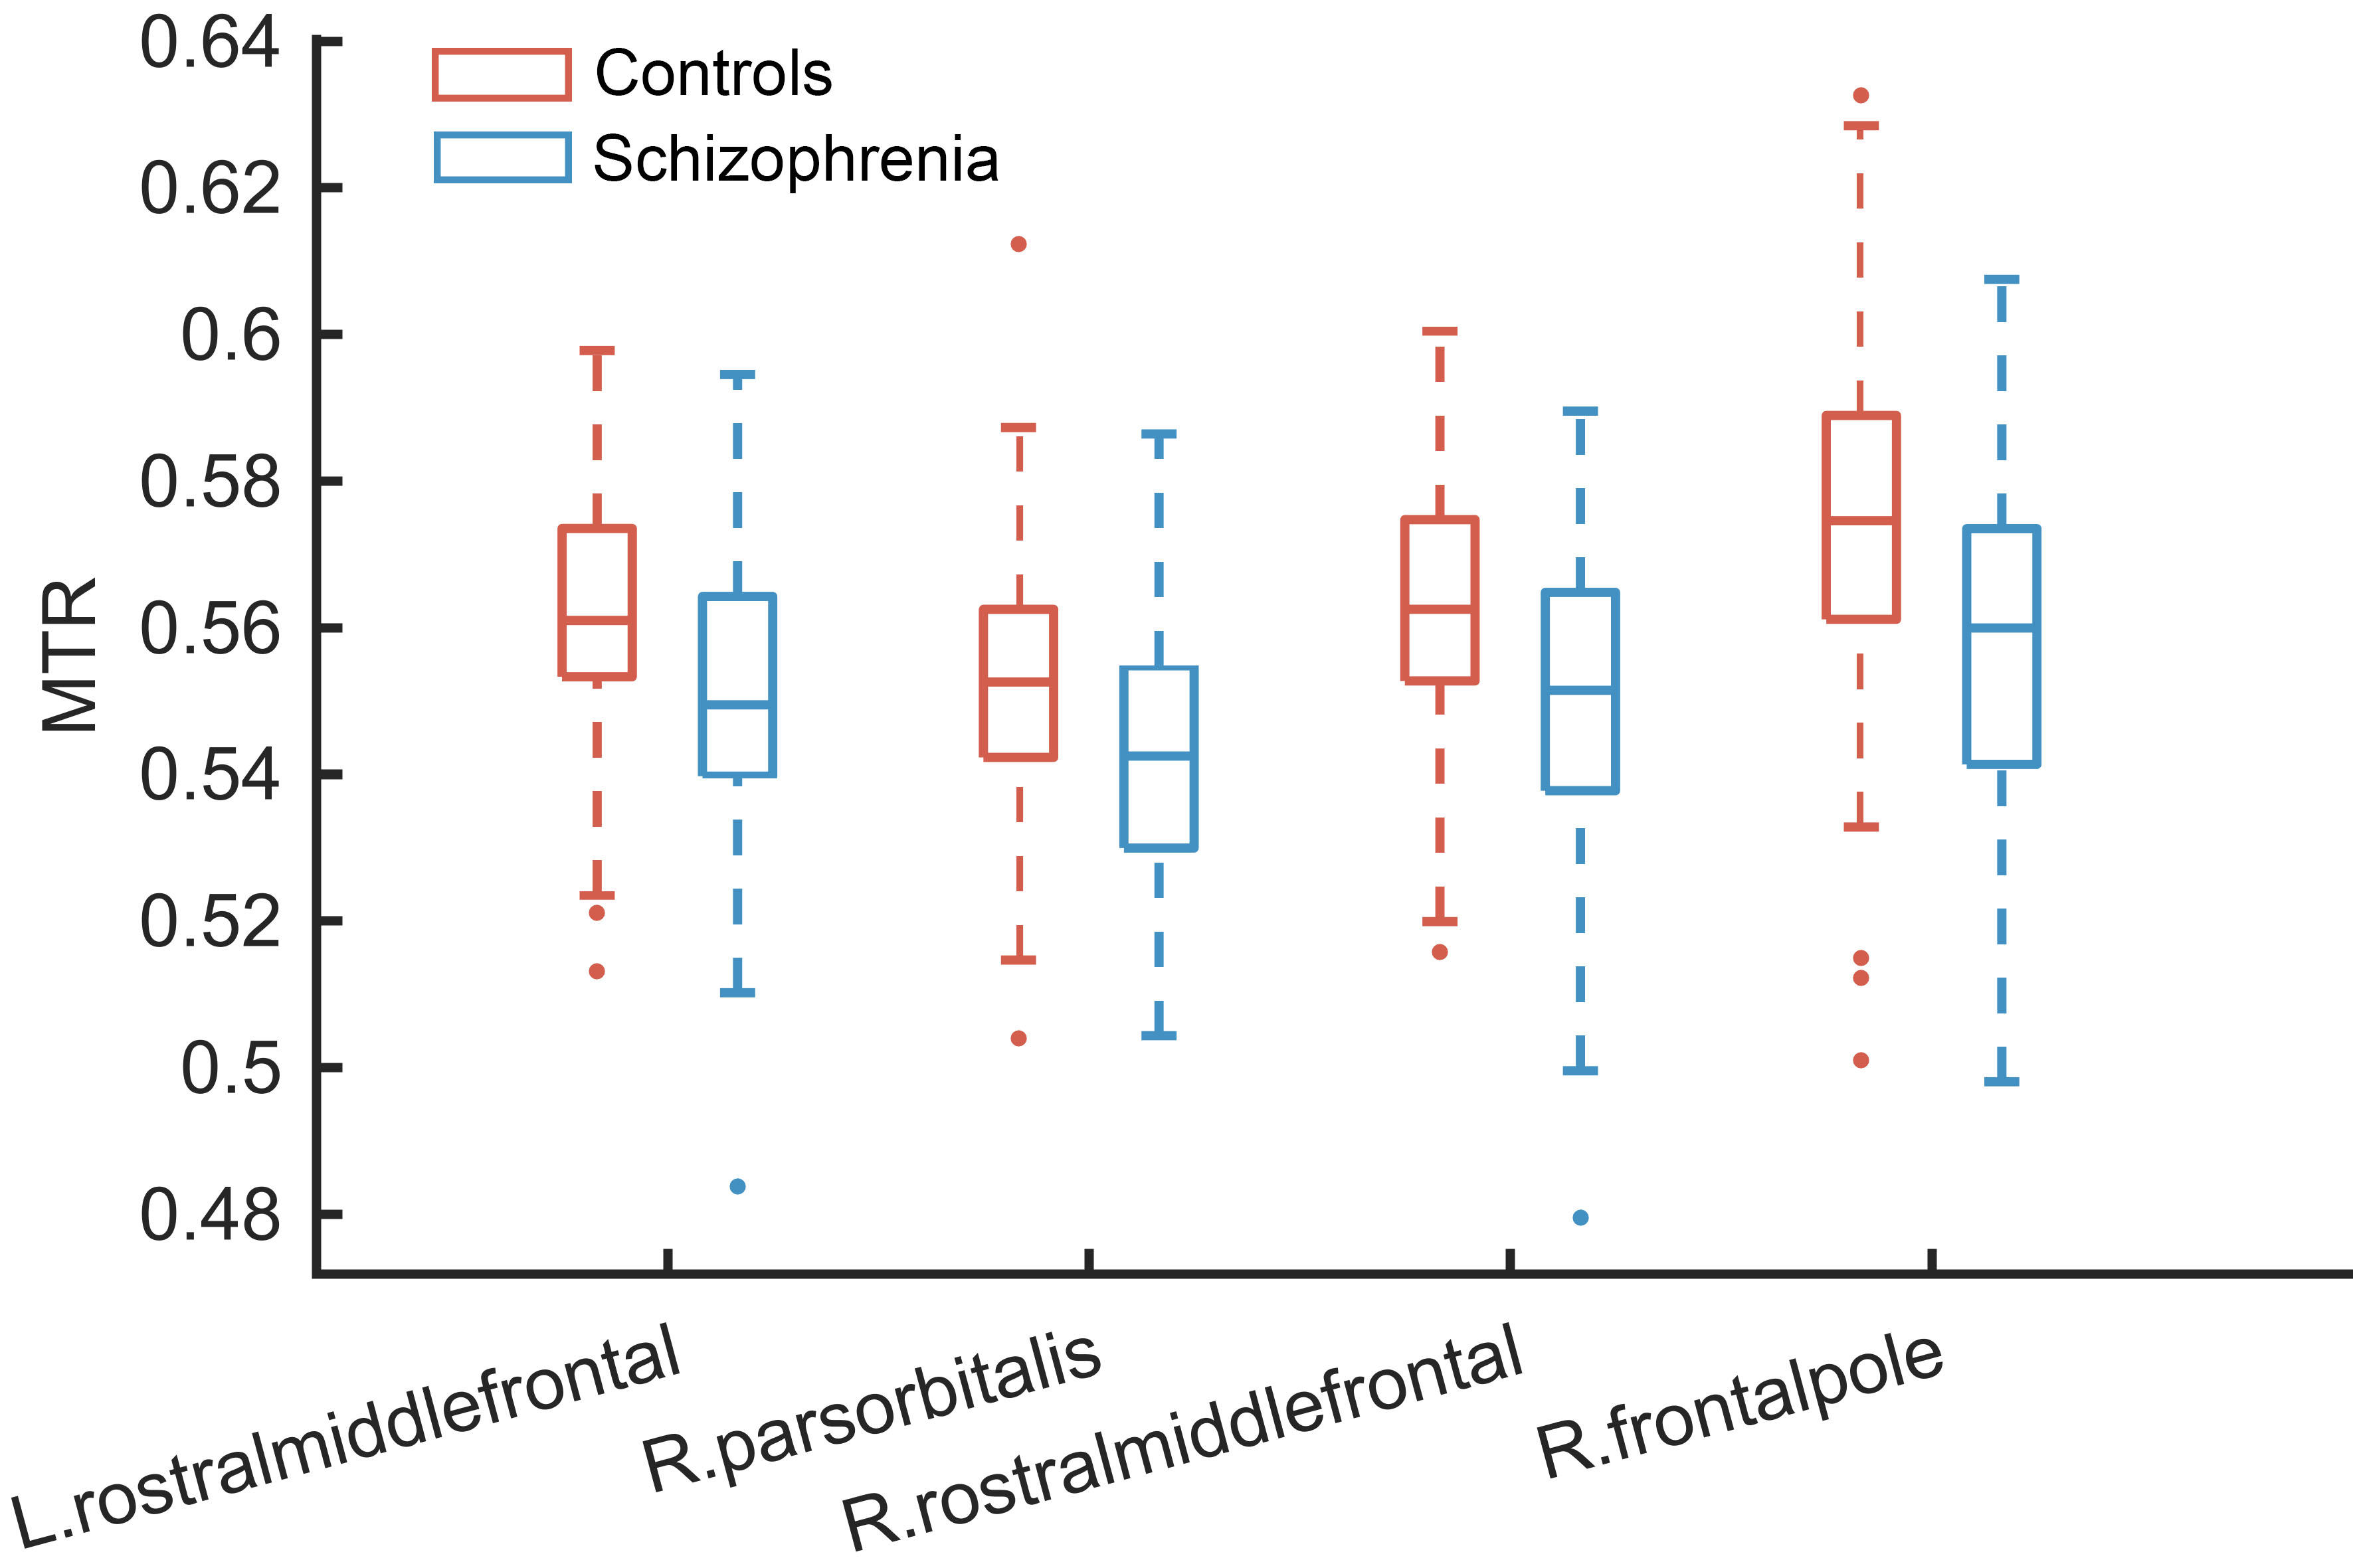
\includegraphics[width=8cm]{images/mtrFig1.jpg}
    \caption{Boxplots of MTR in the bilateral rostral middle frontal area, right pars orbitalis and right frontal pole. The central mark on each box is the median, the edges of the box are the 25th and 75th percentiles, the whiskers extend to the most extreme data points considered not to be outliers according to interquartile range (IQR) algorithm, with outliers plotted individually. Red: controls, blue: schizophrenia patients. L: left hemisphere, R: right hemisphere.}
    \label{mtrFig1}
\end{figure}

\subsection*{Associations between MTR and clinical variables}
Cortical MTR of the regions showing significant MTR differences between schizophrenia patients and controls were tested for associations with clinical symptoms and IQ in patients. There were no significant correlations with positive, negative, total and general PANSS symptoms, nor with IQ and WAIS subtest scores. Only weak correlations were found between the WLT retention rate and cortical MTR in right rostral middle frontal area (\rval = 0.26, \pval = 0.0355, not corrected) and right frontal pole (\rval = 0.28, \pval = 0.0224, not corrected) in schizophrenia patients.

\subsection*{Associations between MTR alterations and disconnectivity}
Cortical maps of MTR alterations and connectivity strength (NOS) changes between schizophrenia patients and controls are illustrated in \ref{mtrFig2}. Regional reductions in MTR were significantly associated with differences in connectivity strength (NOS, \rval = 0.40, \pval < 0.0001) (\ref{mtrFig3}), suggesting that regions with the largest regional MTR reductions also show the largest reductions in macroscale connectivity strength. Examining streamline density yielded similar results (\rval = 0.40, \pval < 0.0001) (Figure 4).

\begin{figure}[h]
    \centering
    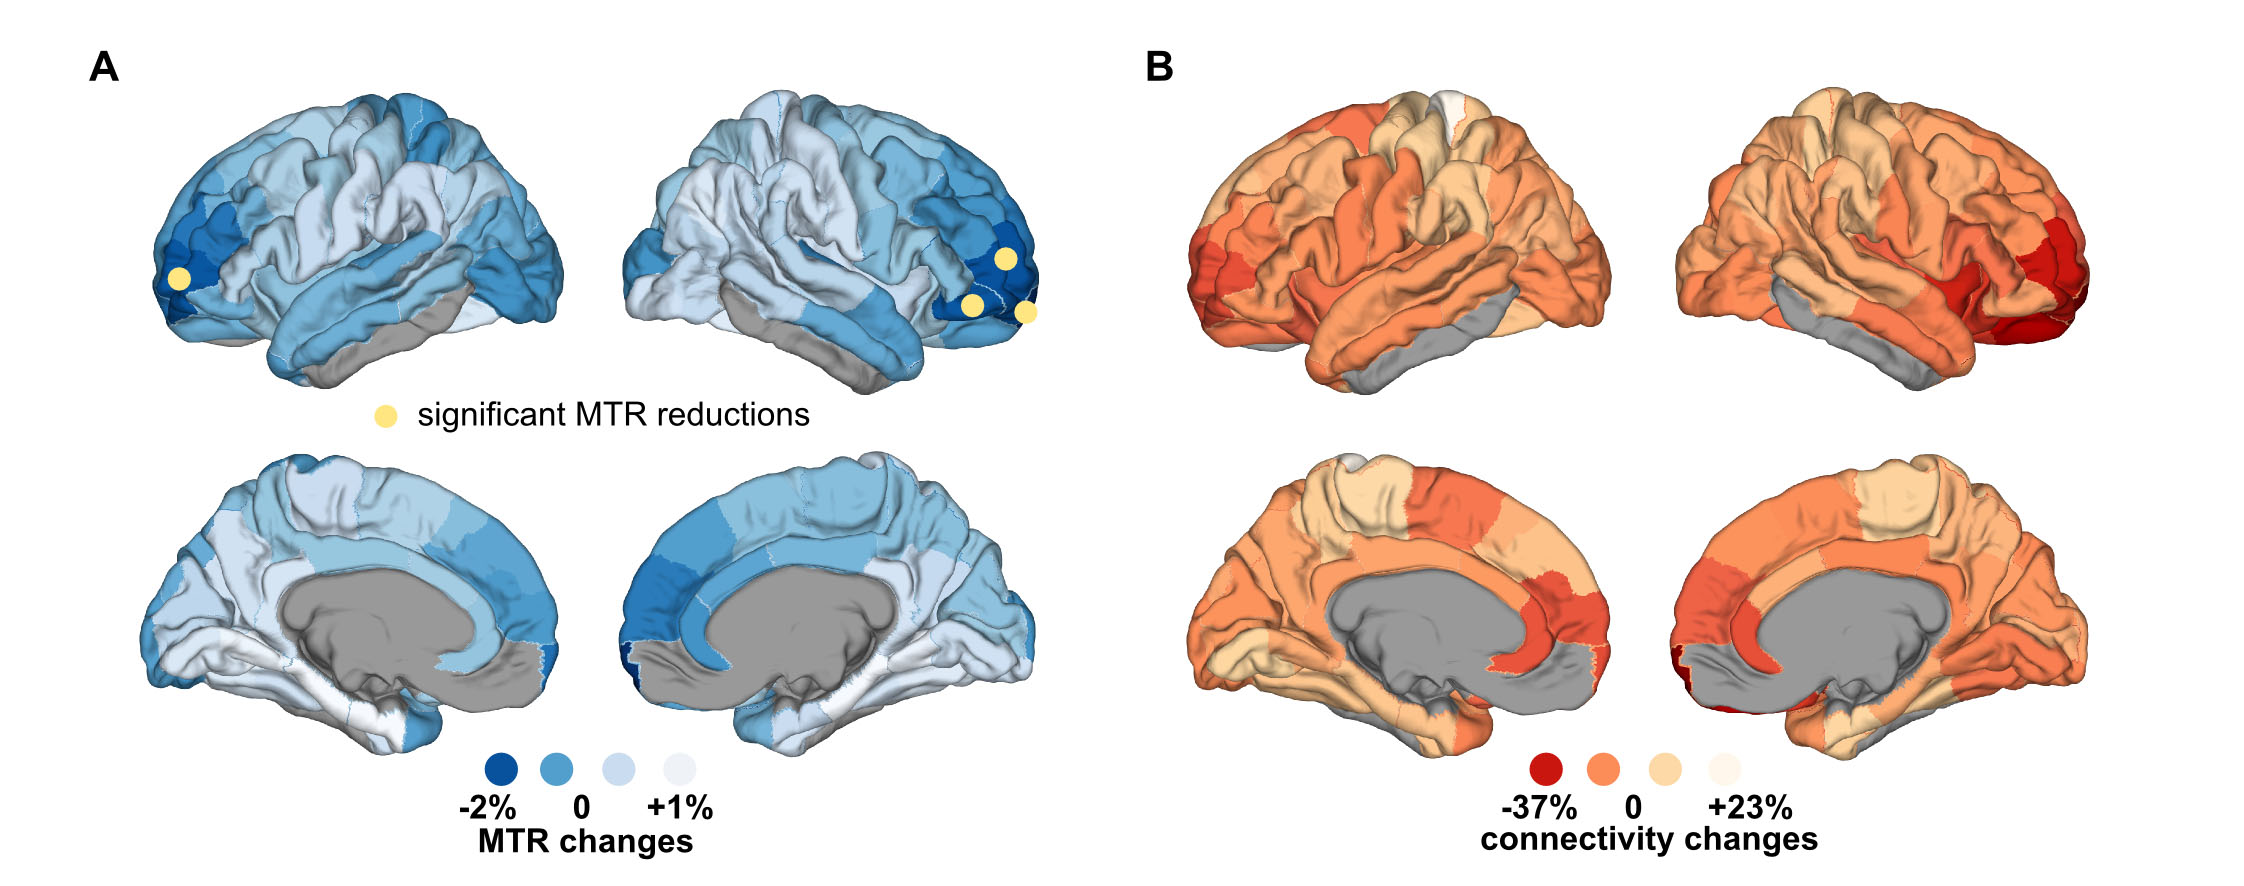
\includegraphics[width=\linewidth]{images/mtrFig2.jpg}
    \caption{Surface maps of between-group changes in MTR and connectivity strength (NOS). (A) Changes for group-averaged MTR between schizophrenia patients and controls (i.e., {[}Patient – Control{]}/Control) are illustrated. Yellow dots indicate cortical regions showing significant MTR differences between the two groups; (B) Changes for group-averaged connectivity strength (NOS) between schizophrenia patients and controls are presented.}
    \label{mtrFig2}
\end{figure}

\begin{figure}[h]
    \centering
    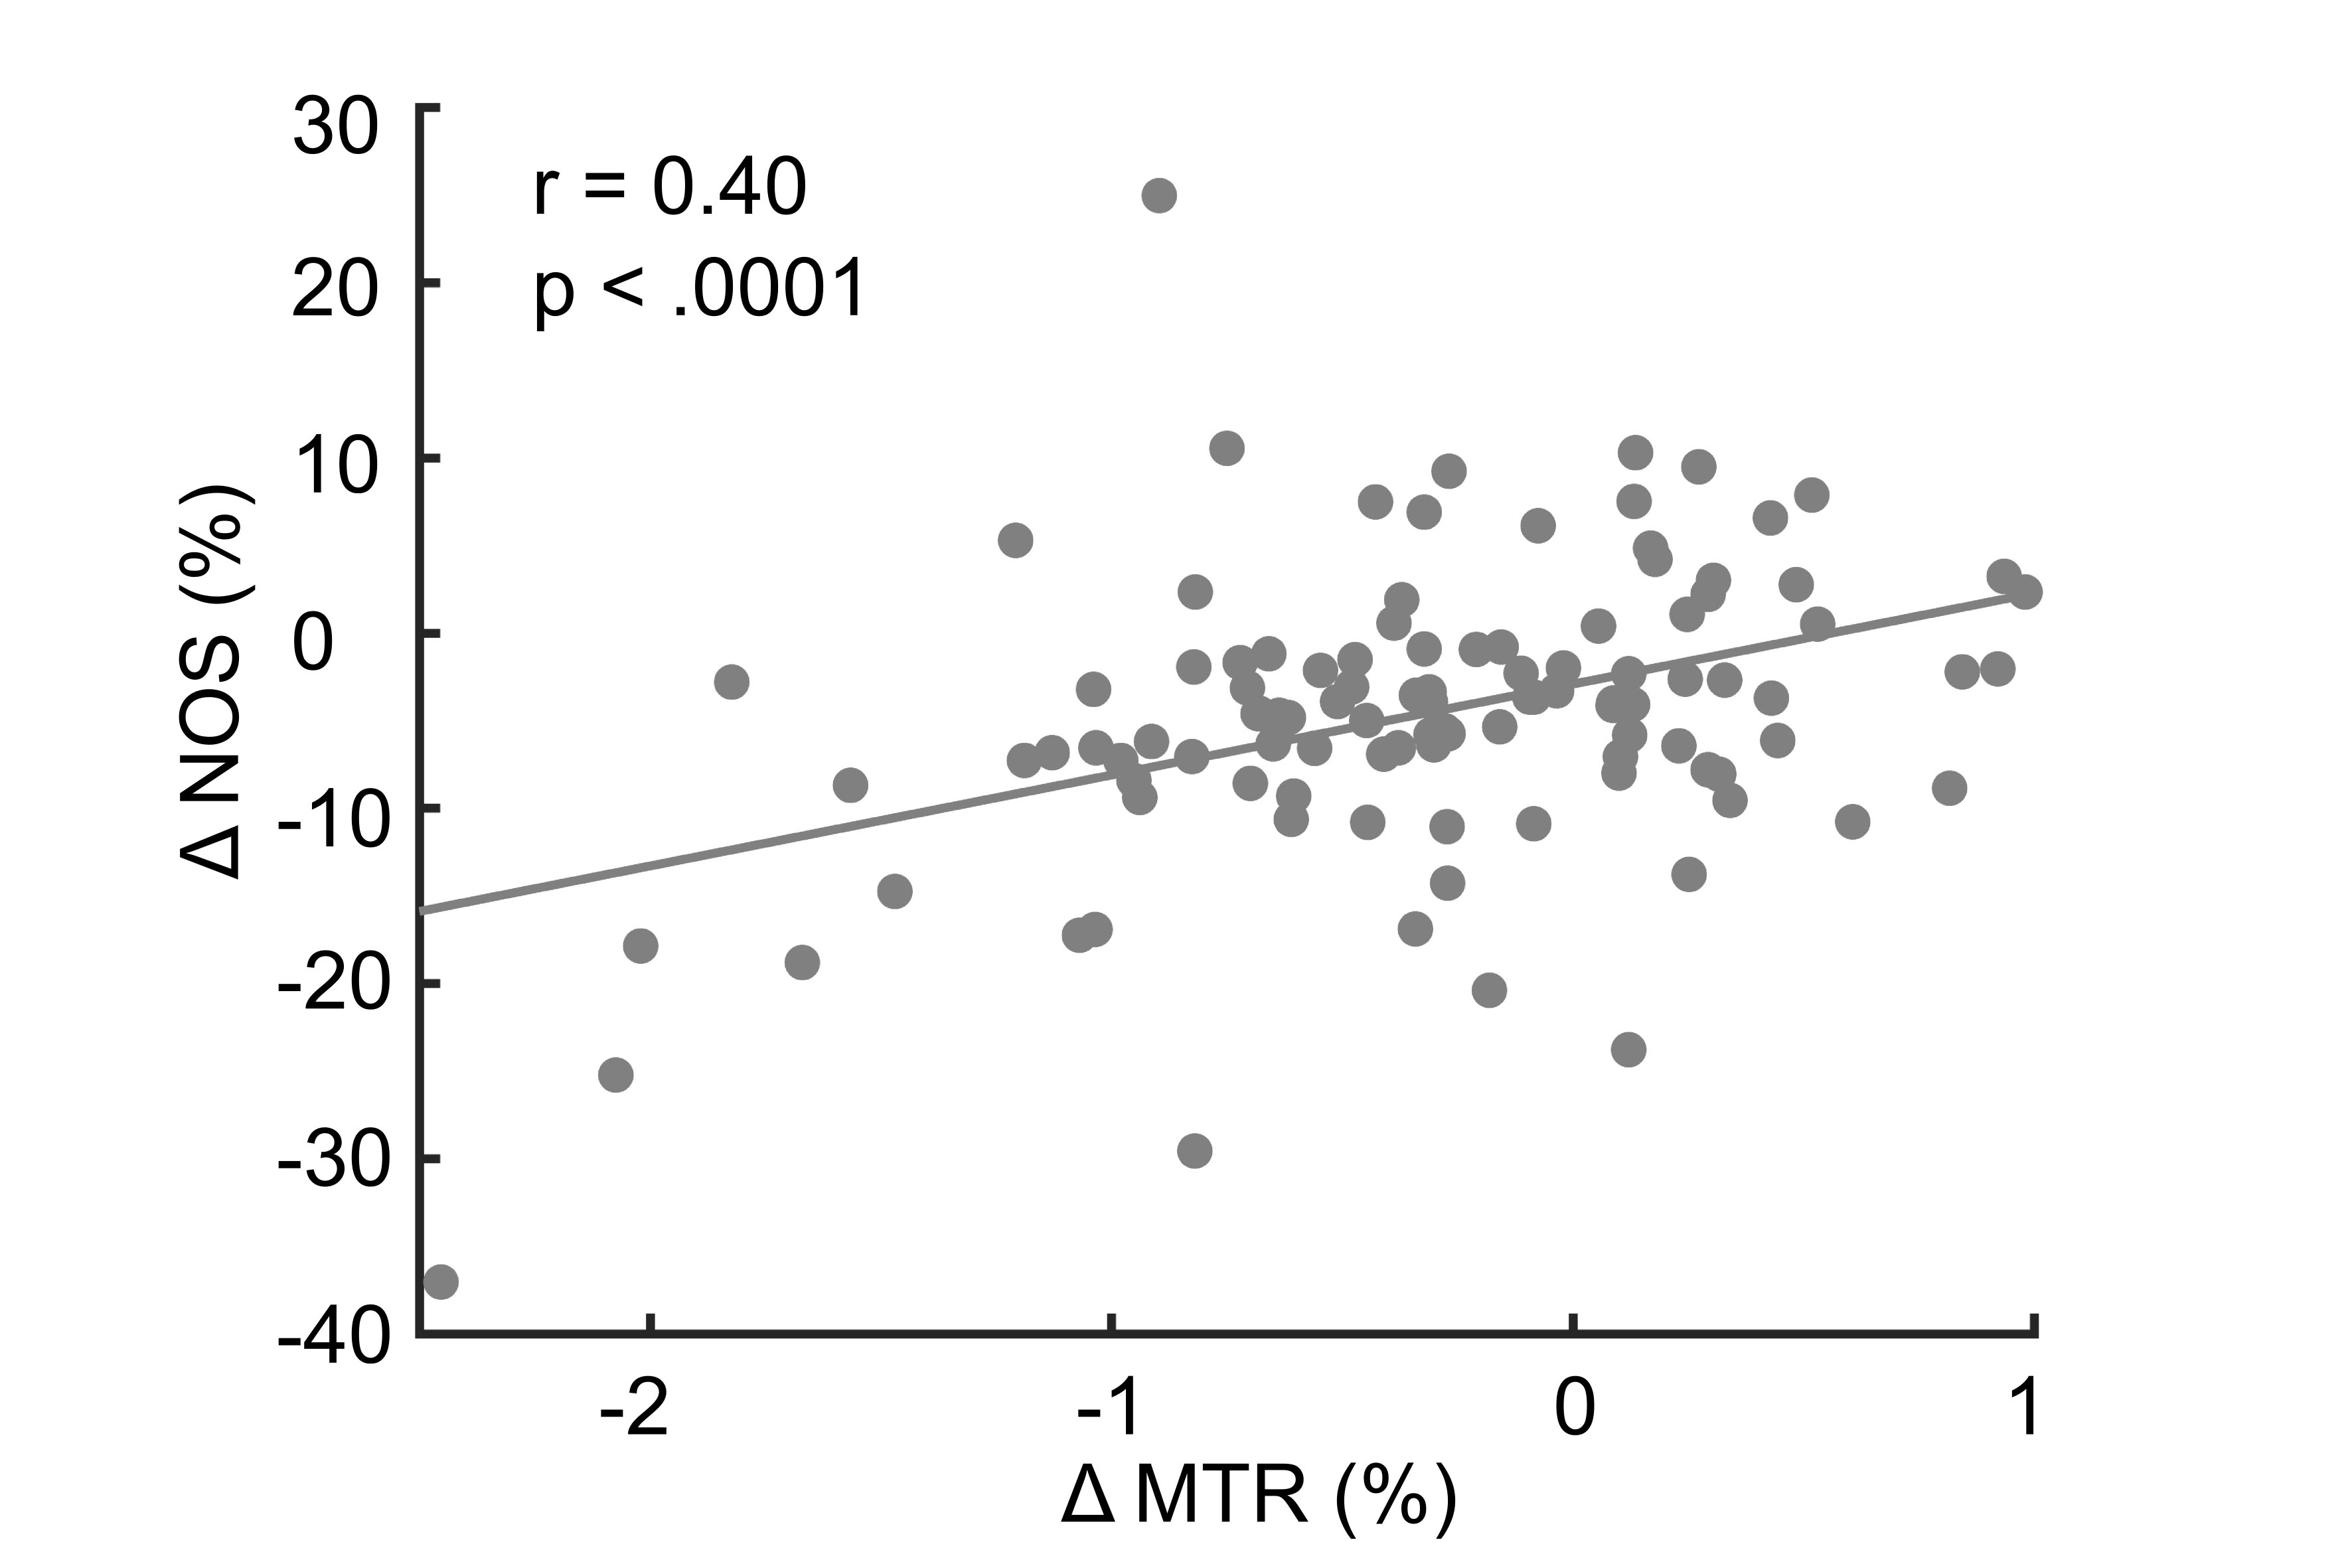
\includegraphics[width=8cm]{images/mtrFig3.jpg}
    \caption{Association between MTR alterations (i.e. $\Delta$ MTR) and connectivity strength changes. $\Delta$ MTR was calculated as the change in group-averaged MTR between schizophrenia patients and controls (i.e., {[}Patient – Control{]}/Control). Changes in cortical connectivity strength are represented by the change in total number of streamline ($\Delta$ NOS) (\rval = 0.40, \pval < 0.0001).}
    \label{mtrFig3}
\end{figure}

\begin{figure}[h]
    \centering
    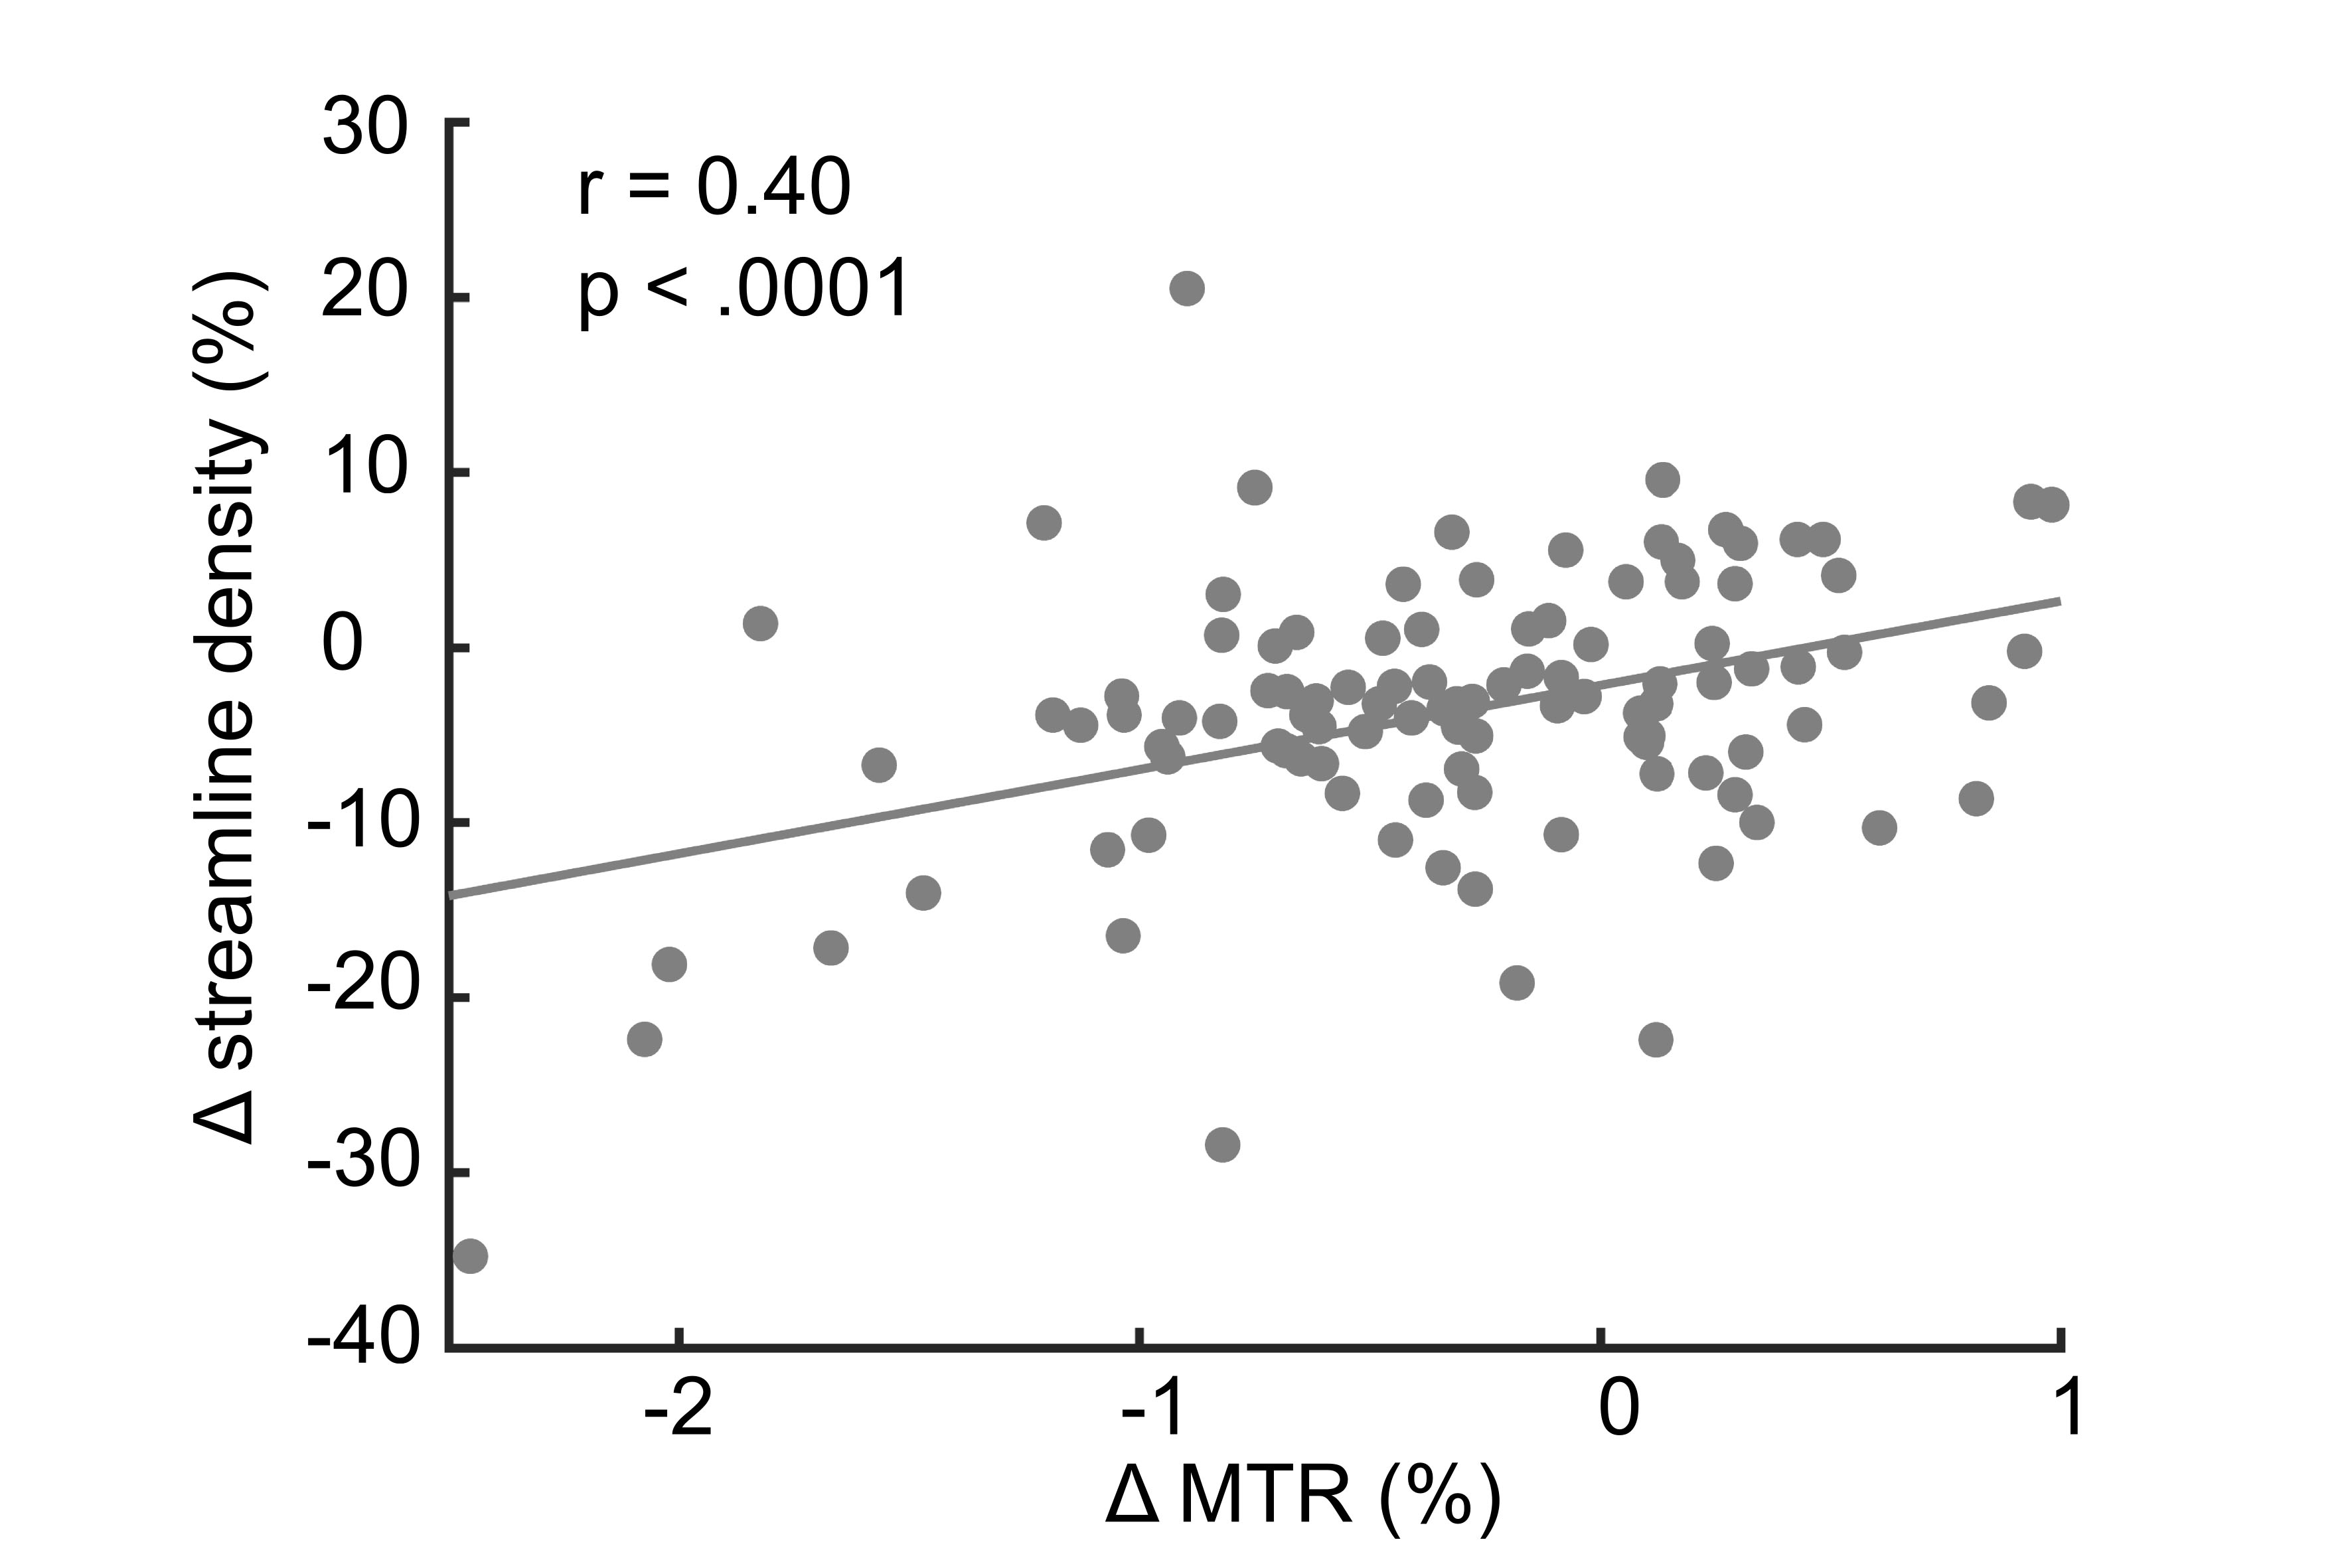
\includegraphics[width=8cm]{images/mtrFig4.jpg}
    \caption{Association between MTR alterations (i.e. $\Delta$ MTR) and connectivity strength changes. $\Delta$ MTR was calculated as the change in group-averaged MTR between schizophrenia patients and controls (i.e., {[}Patient – Control{]}/Control). Changes in cortical connectivity strength are represented by the change in total streamline density ($\Delta$ streamline density) (\rval = 0.40, \pval < 0.0001).}
    \label{mtrFig4}
\end{figure}

Findings persisted when we took changes in cortical thickness and cortical volume into account (NOS: \rval = 0.38, \pval < 0.0001; streamline density: \rval = 0.39, \pval < 0.0001). We alternatively used ranksum values resulting from Wilcoxon Rank Sum test as measurements for between-group differences of MTR and connectivity strength. Regional reductions in MTR consistently showed a significant association with differences in connectivity strength (NOS: \rval = 0.37, \pval = 0.0001; streamline density: \rval = 0.33, \pval = 0.0006). Including changes in cortical thickness and cortical volume as covariates showed similar results (NOS: \rval = 0.34, \pval = 0.0003; streamline density: \rval = 0.31, \pval = 0.0011).


\section*{Discussion}
The present study reveals significant cortical MTR abnormalities in prefrontal cortical areas in schizophrenia, including bilateral rostral middle frontal areas, the right pars orbitalis, and the right frontal pole, suggestive of a prefrontal disruption of macromolecules such as myelin. Second, the cortical pattern of MTR reduction was found to be associated with regional decreases in the level of white matter connectivity in schizophrenia patients relative to controls. These findings provide empirical evidence for microstructural cortical abnormalities of the prefrontal cortex in schizophrenia and suggest that deficits on the microscale are associated with alterations in macroscale structural connectome architecture.\\

The observed prefrontal MTR abnormalities are compatible with prior cytoarchitectural and myeloarchitectural findings in schizophrenia. Decreased neuronal size of layer III pyramidal neurons has been reported in the prefrontal area (e.g., Brodmann area [BA] 9) in schizophrenia \citep{Pierri2001DecreasedSS,Rajkowska1998NeuronalAG}. Moreover, the density of oligodendroglial cells, which are responsible for forming myelin sheath around axons, has been shown to be reduced in BA 9 and BA 10 in schizophrenia \citep{Hof2003LossAA,Uranova2001ElectronMO,Uranova2004OligodendroglialDI}. The frequency of pathologically myelinated fibers has been reported to be significantly increased in prefrontal area BA 10 in schizophrenia patients \citep{Uranova2011UltrastructuralAO} and gene studies further reported reduced expression of myelin-related and oligodendrocyte-related genes in the prefrontal cortex of patients with schizophrenia \citep{Pierri2001DecreasedSS,Mimmack2002GeneEA,Pongrac2002GeneEP}. As MTR is thought to be reflective of macromolecular structures in the cortex such as myelin and cell membrane \citep{wolff1994magnetization}, MTR reductions observed in the current study may be related to these microstructural disruptions in schizophrenia. Hence, our findings provide additional in vivo evidence for neuropathological abnormalities in the prefrontal cortex in schizophrenia. \\

MTR abnormalities in schizophrenia are observed to be correlated with alterations in white matter connectivity in our study. This provides indirect support for a relationship between histological features of cortical microsctructure and macroscale connectivity. Macroscale topological properties of white matter connectivity have been reported to be associated with spine count and density of cortical layer III pyramidal neurons \citep{VANDENHEUVEL2016293} and layer III neuronal size \citep{Heuvel2015BridgingCA} in the healthy human brain. Furthermore, alterations in macroscale white matter connectivity in schizophrenia patients were correlated with changes in spine density of cortical layer III pyramidal neurons \citep{VANDENHEUVEL2016293}. These findings indicate that disruptions in macroscale white matter connectivity may reflect long-range axon abnormalities that accompany cortical microscale connectivity changes. Brain disconnectivity in schizophrenia has been hypothesized previously to be related to myelination disruptions caused by reduced oligodendrocytes \citep{Cassoli2015DisturbedMI}, due to myelin regulate the velocity and synchrony of inter-cortical impulse conduction \citep{Fields2008WhiteMI}. Our findings may provide empirical evidence for this micro-macro association, showing cortical regions with myelination disruptions as revealed by in vivo MTR to be related to the pattern of macroscale disconnectivity in schizophrenia. \\

The underlying processes that drive the observed association between MTR abnormalities and white matter connectivity disruptions in schizophrenia remains to be determined. It is known that the streamline number or density measured by diffusion MRI can reflect multiple microscale characteristics, such as axonal number, density, caliber, or myelination \citep{Jones2013WhiteMI}. One hypothesis to explain the MTR-connectivity association could be that reduced white matter connectivity reflects a reduced number or density of axons, which may lead to a decreased intra-cortical myelin content revealed by MTR. Alternatively, pathologically altered intracortical myelination may disrupt neural impulse conduction, and thereby lead to pruning of axons revealed by macroscale connectivity strength. Furthermore, a rich body of literature has reported longitudinal disease effects on both the microscale and macroscale of brain organization \citep{Bullmore1997TheDN,Catani2005TheRA}. The observed association may thus also reflect a more complex bidirectional process of interactions between microstructural abnormality in gray matter and macroscale disconnectivity during the course of disease. \\

The putative impact of cortical thinning \citep{Goldman2009WidespreadRO,Haren2011ChangesIC} on our findings was thoroughly examined. We adopted a weighted average measurement for MTR that minimizes the contribution of voxels located in the boundaries of the cortical ribbon. Cortical thickness and volume were regressed out from MTR during statistical analysis. In addition, the validation analysis of the potential cortical thinning effect on MTR between subgroups divided by cortical thickness did not change the results (see Supplementary Information), further indicating that our MTR findings are likely to be independent of cortical thinning effects. \\

Several other comments have also to be made when interpreting the findings of our study. First, most patients (>85\%, see 2.1. Subjects) received antipsychotic treatment that might affect the intracortical MTR metric. Examining the relationship between antipsychotic medication dosage and MTR, we found no significant correlations, suggesting that our findings are unlikely driven by antipsychotic medication use. Second, there was a male predominance in the patient group. Post-hoc comparisons revealed MTR reductions between schizophrenia patients and controls in males only, but not in females (see Supplementary Information). This may be due to the small sample size of female patients (N = 14) included in our study, or may reflect stronger effects in male as compared to female patients. After randomly excluding female controls to make the gender distribution matched, we consistently found significant MTR reductions in the four reported prefrontal regions (see Supplementary Information), indicating that our findings were likely not driven by a gender effect. Third, the cortical MTR of the four prefrontal areas that showed reductions in schizophrenia only weakly correlated with the WLT retention rate, but did not correlate with other clinical symptoms and cognitive variables. It is probably because of the fluctuating nature of clinical symptoms that change with psychotic episodes and remissions, while MTR findings represent structural deficits that may reflect an underlying neurobiological vulnerability. Finally, given that the included data is part of a long running clinical cohort, the MTR and DWI data included relatively low resolution data acquired on a 1.5 T clinical scanner. Nevertheless, we noticed that MTR data showed acceptable reliability because of high tissue contrasts, high signal to noise ratios, and relatively low within-subject signal variances (see Supplementary Information). Future studies deploying high-field imaging will enhance image quality with higher resolution and higher signal to noise ratios, which may result in less partial volume effects for MTR extraction and better detection of white matter tracts in DWI. \\

This study shows significant MTR reductions in prefrontal cortex areas in schizophrenia patients and a significant association of MTR abnormalities with alterations in white matter connectivity in schizophrenia. Our findings provide in vivo support for cytoarchitectural and myeloarchitectural disruptions of the prefrontal cortex in schizophrenia and emphasize a link between microscale neuropathology and disease-related connectome alterations, suggestive of a complex etiology that crosses multiple scales of connectome organization.

\printbibliography[heading=subbibliography]

\end{refsection}

% SI
\newpage
\begin{refsection}
\section*{Supplementary Information}
\subsection*{MTR reliability analysis}
We examined the reliability of MTR signals in three ways, by analyzing tissue contrast, signal to noise ratio (SNR), and individual variance in MTR signals. First, we extracted the mean MTR signal within distinct brain tissues (i.e., gray matter, white matter and CSF) for each subject. As shown in Figure S1, the mean MTR signals in gray matter (0.5522 $\pm$ 0.0095) were lower than signals in white matter (0.6020 $\pm$ 0.0086), but substantially larger than signals in CSF (0.2384 $\pm$ 0.0451), indicating reliable signal contrast in MTR images.

Second, we calculated the SNR based on MTR signals extracted in the gray matter for each subject. SNR was defined as the ratio of the mean ($\mu$) to the standard deviation ($\sigma$) of the MTR signal:

\[SNR = \frac{\mu}{\sigma} \]

We found that the SNR ranged from 6.60 to 15.05, with a mean value of 10.26, consistent with an acceptable SNR level according to the Rose criteria, which define scans with SNR $\geq$ 5 as acceptable \citep{Bushberg2011TheEP}.

Third, we computed within-subject MTR variance for each dataset as follows:

\[VAR_{within-subject} = \frac{1}{N-1}\sum_{i=1}^{n}(MTR_{i}-\mu)^{2}\]

where N is the number of cortical regions, MTR\textsubscript{i} the mean MTR within region \textit{i}, and $\overline{\mu}$ the mean MTR among all cortical regions. Likewise, between-group MTR variance was calculated for each cortical region:

\[VAR_{between-group} = \frac{1}{N_{groups}-1} \sum_{i=1}^{N_{groups}} n_{i}(\overline{\mu}_{i} - \overline{\mu})^2\]

where N\textsubscript{groups} is the number of groups (here, N\textsubscript{groups} = 2), n\textsubscript{i} the number of subjects in the group i, $\overline{\mu}_{i}$ the mean MTR in subjects of the group i, and $\overline{\mu}$ the mean MTR in all subjects. We found that the VAR\textsubscript{within-subject} ranged from 0.0001 to 0.0010 in schizophrenia patients and from 0.0001 to 0.0011 in controls (Figure S2). VAR\textsubscript{between-group} of the four regions showing significant MTR reductions in patients (i.e., the bilateral rostral middle frontal area, the right pars orbitalis, and the right frontal pole) ranged from 0.0040 to 0.0094, which is 13 to 31 times larger than the average VAR\textsubscript{within-subject}. These findings show that MTR differences between schizophrenia patients and controls are much larger than within-subject MTR measurement variance.

\subsection*{Validation analysis: potential effect of cortical thinning}
We performed a reliability analysis to examine whether cortical thinning effects were not driving the MTR group-effect shown in the main text. To this end, for each region showing a significant between-group MTR difference, we ordered subjects according to cortical thickness and split each group into two subgroups, i.e. schizophrenia patients with above-average thickness (n = 38) and with below-average thickness (n = 37), as well as controls with above-average thickness (n = 45) and with below-average thickness (n = 44). Wilcoxon Rank Sum permutation analyses were performed to compare regional MTR measurements between each set of subgroups. We found no MTR differences between patients (or controls) with above-average thickness versus patients (or controls) with below-average thickness (\textit{p}s > 0.1292). Moreover, comparing controls with below-average thickness to patients with above-average thickness again showed MTR reductions in the four prefrontal regions (i.e., bilateral rostral middle frontal area (\pval = 0.0001 and 0.0197), right pars orbitalis (\pval = 0.0264), and right frontal pole (\pval = 0.0022)), indicating that cortical thinning effects are not driving group-effects in MTR.

\subsection*{Gender effects on MTR findings}
We examined the effects of group-gender differences on our MTR findings in two ways, as there was a higher proportion of males in the patient group (e.g., 42 males and 47 females in controls, 62 males and 14 females in patients, $\chi^{2}$ = 20.80, \pval < 0.0001). First, Wilcoxon Rank Sum permutation analyses, which estimate the difference between medians of the two groups, were performed between cortical MTR of schizophrenia patients and controls in male and female subjects only. This analysis confirmed MTR reductions in the bilateral rostral middle frontal area, the right pars orbitalis, and the right frontal pole between 62 male patients and 42 male controls (\pval = 0.0090, 0.0010, 0.0007, and 0.0078, separately) (Figure S3). The effects were remained in left rostral middle frontal area (p = .0222) when comparing the 14 female patients to 48 female controls, but not in other three regions (\pval = 0.1892, 0.1858, and 0.1491, separately), which may be due to either weaker group-effects in female subjects or reduced sample size and power (i.e., testing only 14 female patients). To investigate whether there is a general gender-related MTR difference, the same analysis was also conducted in 42 male controls and 48 female controls. We found no MTR differences in bilateral rostral middle frontal area (\pval = 0.1296 and 0.1196) or right pars orbitalis (\pval = 0.7230), but a trend towards higher MTR values in female controls for the right frontal pole (\pval = 0.0244). These findings suggest that there may be subtle gender-related differences in MTR for some brain regions, but show that our main group-effects in MTR is not driven by group-differences in gender distribution.

Second, we reassessed MTR group-differences using a subgroup of gender-matched controls. We randomly excluded 37 female controls to obtain a gender-matched subgroup (patients: 62 males/14 females; controls: 42 males/10 females, $\chi^{2}$ = 0.01, \pval = .9082) and redid the between-group MTR comparison. The randomization process was repeated for 1000 times and p values for the four significantly different prefrontal regions in our primary analysis (i.e., bilateral rostral middle frontal area, right pars orbitalis, and right frontal pole) were recorded for each randomization. MTR reductions were found in 964 of the 1000 randomizing trials for all those four regions, further supporting that the main group-effects in MTR is not driven by gender effect.

\subsection*{Supplementary References}
\printbibliography[heading=none]

\newpage
\subsection*{Supplementary Figures}
\begin{figure}[H]
\centering
  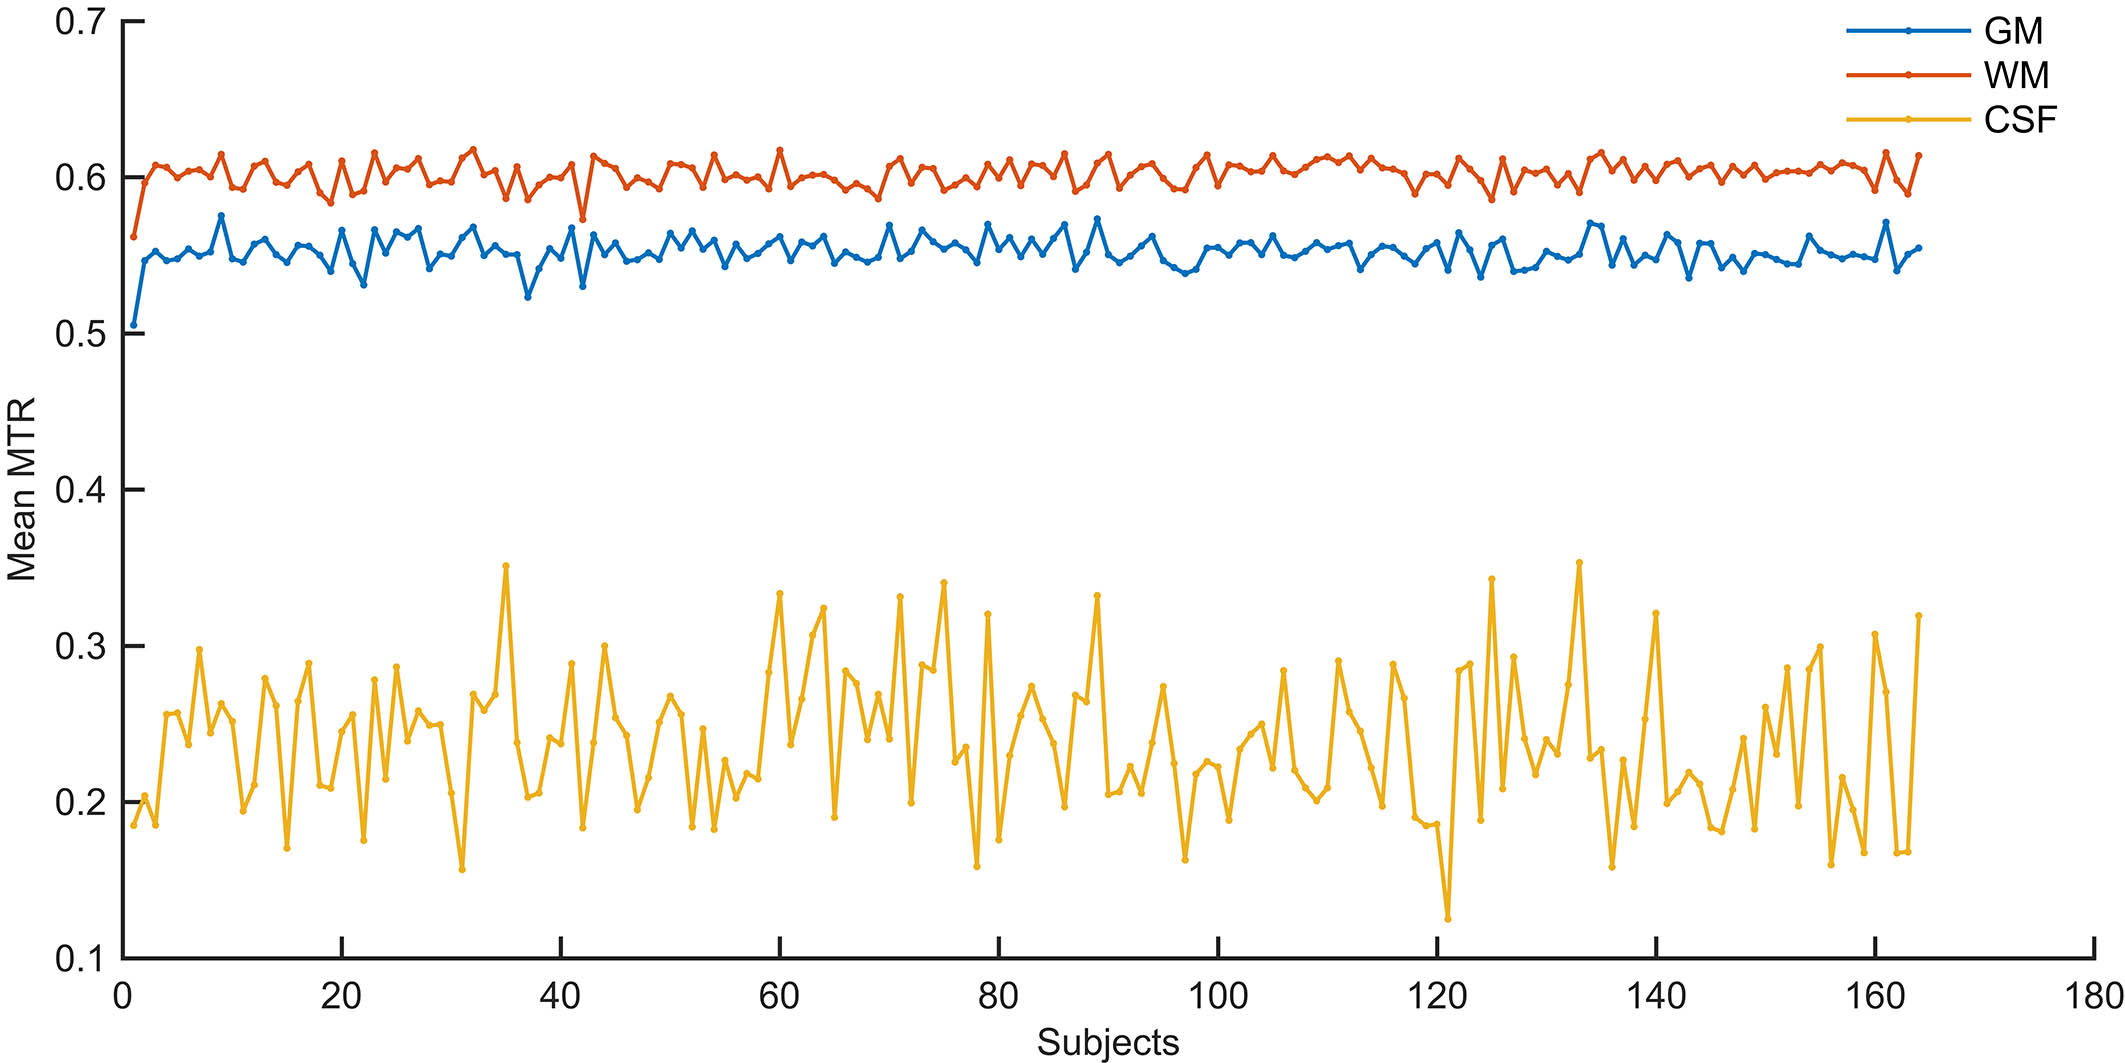
\includegraphics[width=\linewidth]{images/mtrFigS1.jpg}
  \caption{\small Mean MTR signals within gray matter, white matter and CSF for each subject. Blue: gray matter; red: white matter; yellow: CSF.}
  \label{mtrFigS1}
\end{figure}

\begin{figure}[H]
\centering
  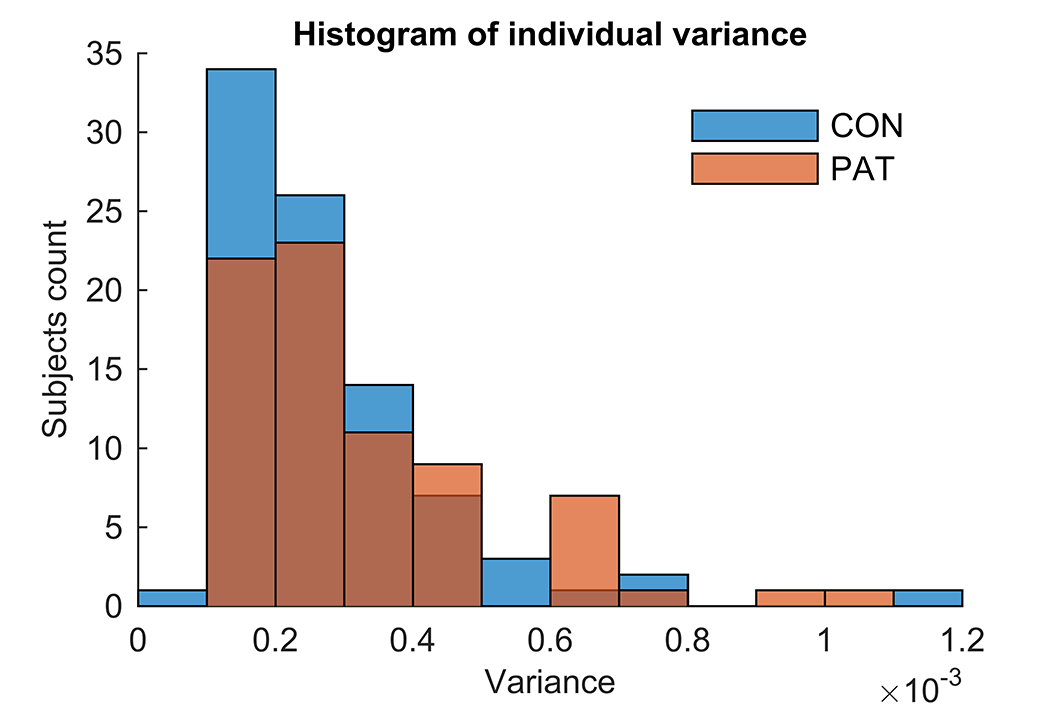
\includegraphics[width=8cm]{images/mtrFigS2.png}
  \caption{\small Histogram of within-subject variances for MTR in each subject. Blue: controls; orange: schizophrenia patients.}
  \label{mtrFigS2}
\end{figure}

\begin{figure}[H]
\centering
  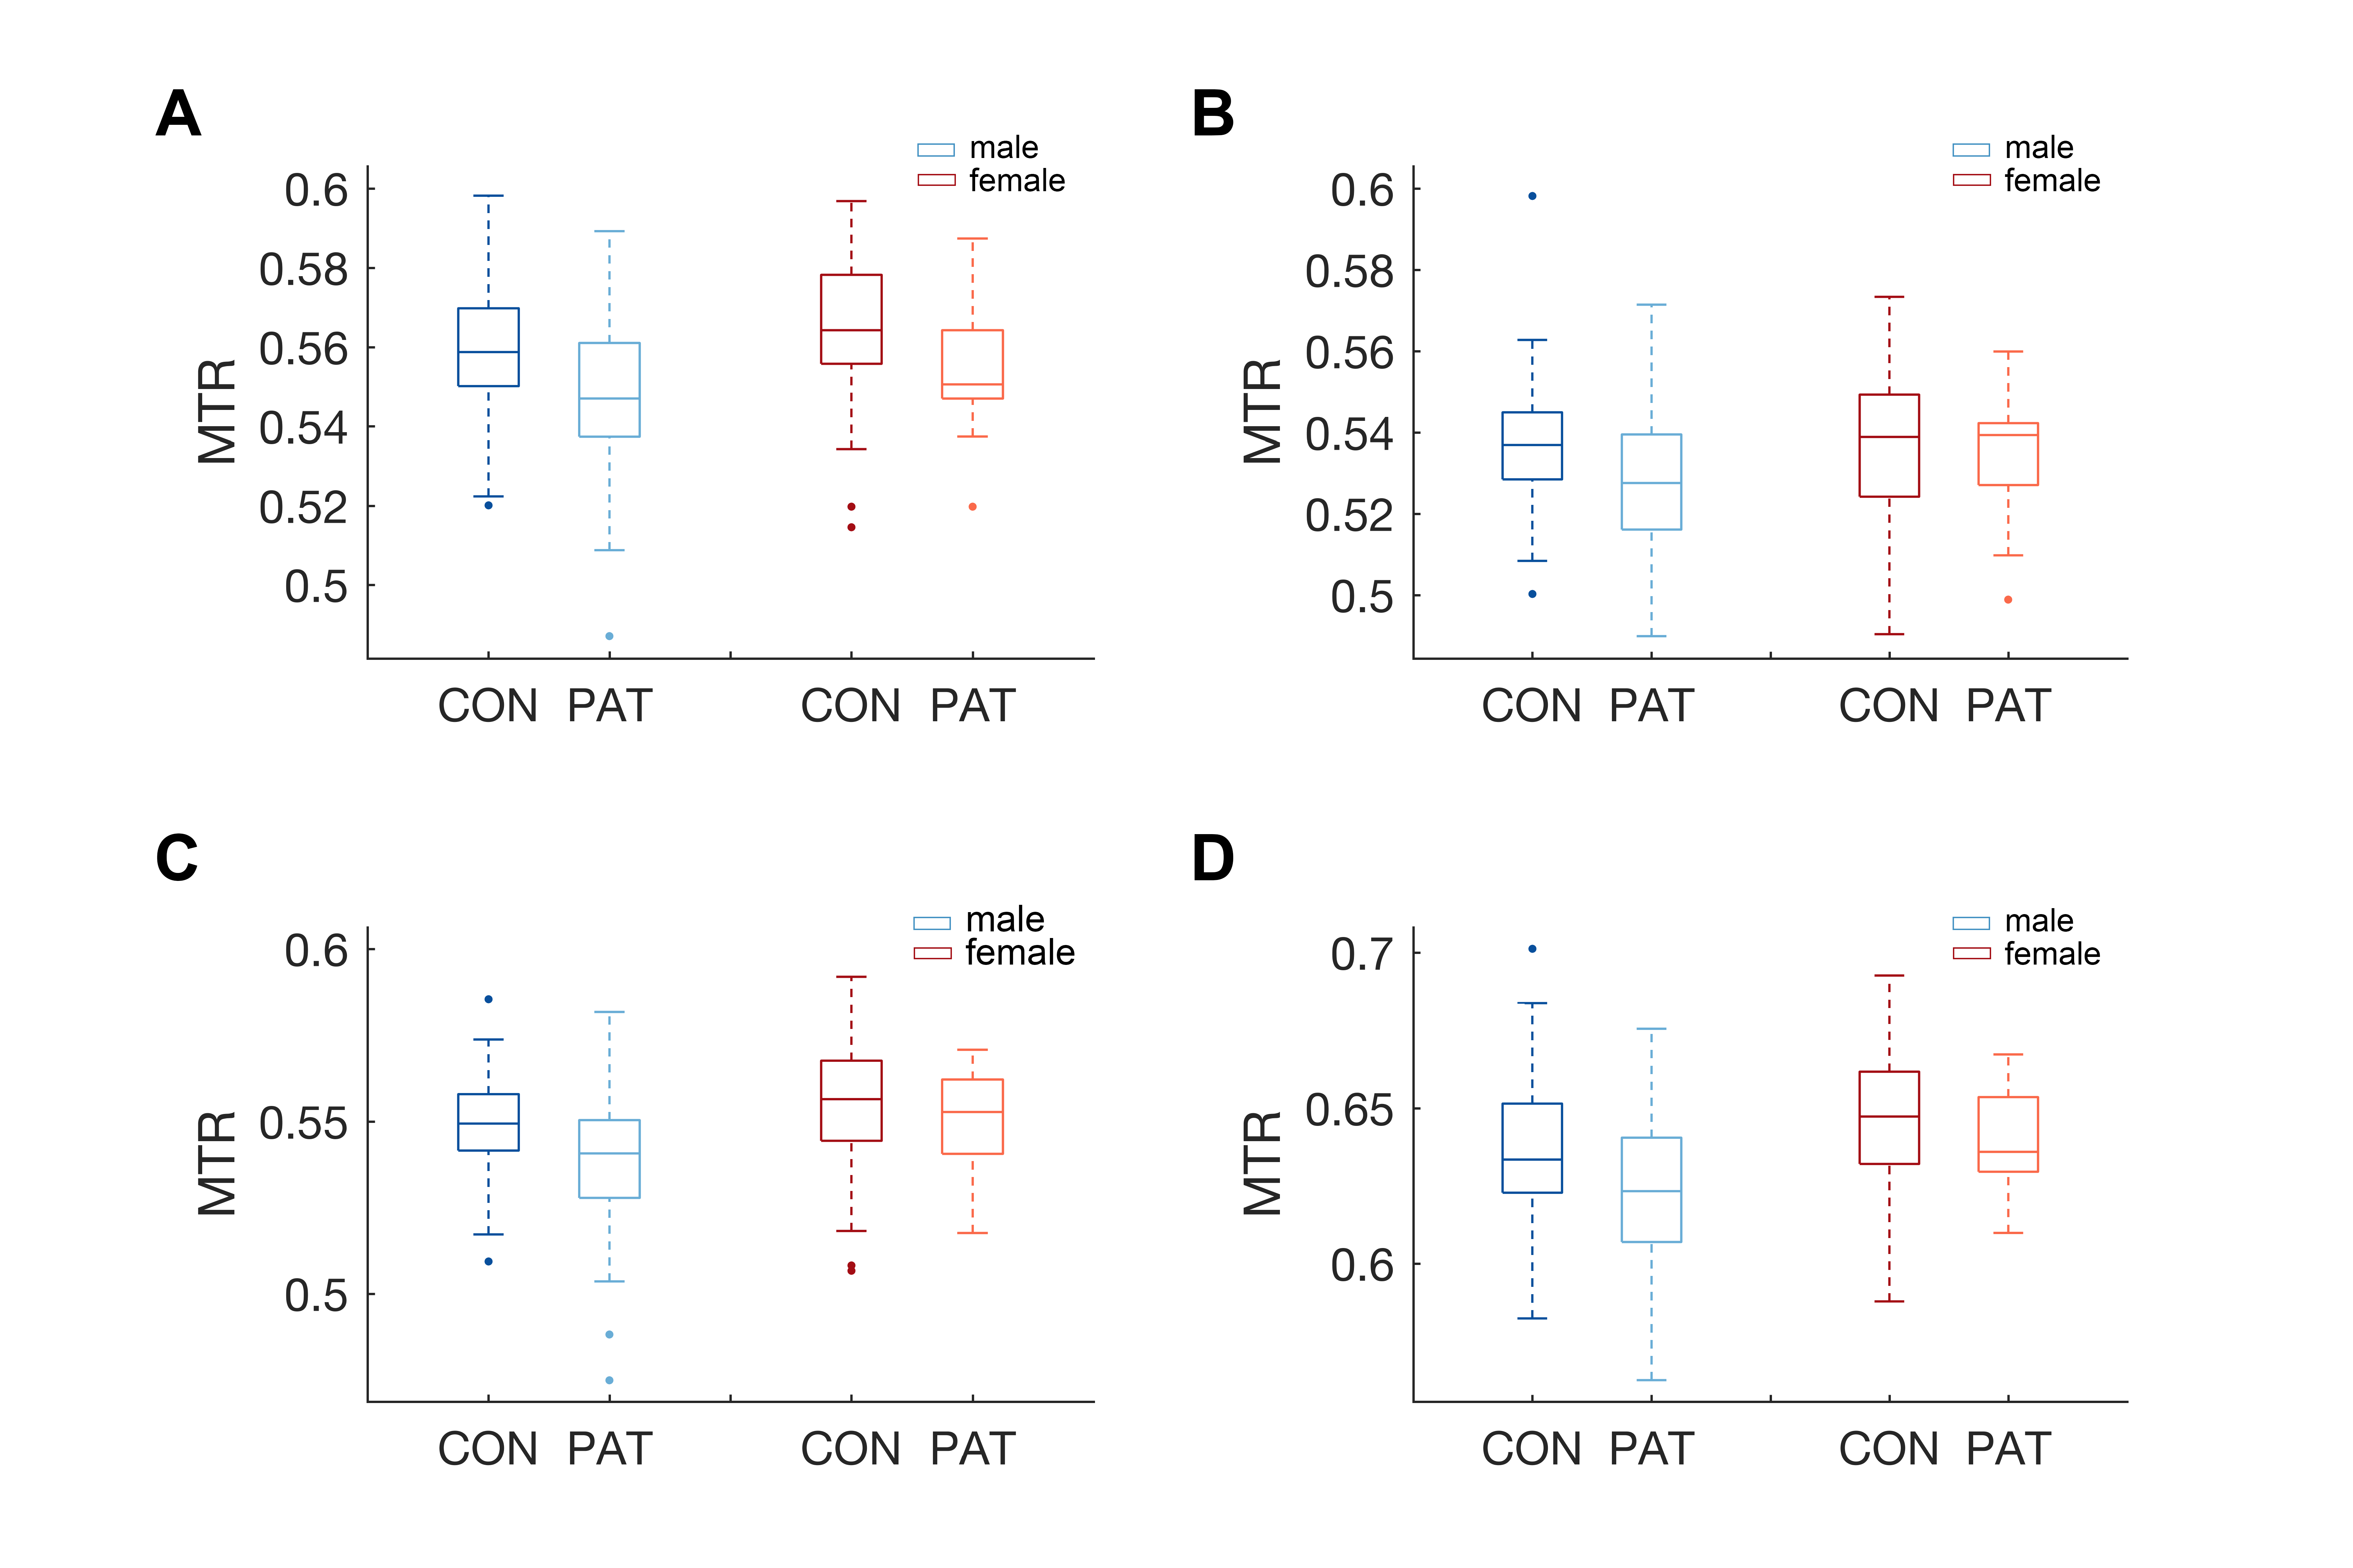
\includegraphics[width=\linewidth]{images/mtrFigS3.png}
  \caption{\small Boxplots of the MTR in the bilateral rostral middle frontal area (left hemisphere: A and right hemisphere: C), right pars orbitalis (B) and the right frontal pole (D). On each boxplot. the central mark on each box is the median, the edges of the box are the 25th and 75th percentiles, the whiskers extend to the most extreme data points considered not to be outliers according to interquartile range (IQR) algorithm, and the outliers are plotted individually. Blue: female, red: male, darker: controls, lighter: patients.}
  \label{mtrFigS3}
\end{figure}



\end{refsection}


% \pagestyle{MyStyle}

\begin{refsection}

\chapter{Summary and general discussion}
\label{ch:summary}

\newpage

In this chapter, I will first summarize the main findings presented in this thesis, followed by a general discussion with a comprehensive literature review. The discussion is categorized into two parts: 1) evidence for multiscale wiring principles of the human brain connectome is incorporated, and 2) observations in the context of multiscale neuropathology of schizophrenia are revisited. Furthermore, limitations and future directions in the field of multiscale connectomics will be deliberated.

\section*{Summary}
Integrating the genetic, histological, and brain imaging data have provided a rich body of evidence for the relationship across multiscale brain connectome organization (Scholtens and van den Heuvel, 2018; van den Heuvel et al., 2019a). Studies on non-human mammalian species have shown that the similarity of the microscale cortical cytoarchitecture is associated with the formation of macroscale cortico-cortical connectivity (Barbas, 2015; Beul et al., 2015; Beul et al., 2017). Chapter 2 provides further evidence for such a micro-macro association by combining the state-of-the-art ultrahigh-resolution BigBrain dataset and the macroscale connectome of the human brain. The laminar cytoarchitectonic profile of human cortical regions was delineated using the BigBrain dataset, and the connectome was reconstructed using diffusion weighted imaging (DWI) data based on homologous cortical regions. Bridging the two ends of scales showed that the cytoarchitectonic profiles were more similar between interconnected cortical regions as compared to non-connected regions. The level of the cytoarchitectonic profile similarity was positively correlated with the connectivity strength, suggesting that cortical regions with more similar cytoarchitecture tend to be connected by stronger white matter connections. These results thus confirm one of the important wiring principles of the connectome – the microscale cortical cytoarchitectonic similarity shapes the macroscale brain connectome organization – to be evolutionarily conserved across multiple species with no exception in the human. 

In Chapter 3, I further demonstrate the wiring principles of brain functional networks from the perspective of evolutionary genetics. In the human brain, there are several functional networks, such as the frontoparietal network (FPN), salience network (SN), and default-mode network (DMN), supporting higher-order brain functions that differentiate human from other intelligent evolutionary relatives (Buckner and Krienen, 2013). We thus hypothesized that brain regions of these higher-order cognitive networks were largely expanded in human evolution and this expansion was influenced by the underlying genetic differences between human and other non-human primates. To test this hypothesis, the cortical ribbon of humans and chimpanzees was first reconstructed using magnetic resonance imaging (MRI) data, and surface area of homologous cortical regions was compared between humans and chimpanzees. This comparison showed the highest cortical expansion in regions of higher-order cognitive networks, such as the FPN and DMN, in the human brain. Next, the pattern of brain expansion was linked to the gene expression pattern of the human-accelerated genes (HAR genes) in the human brain. Brain regions with more expansion in human evolution were found to demonstrate higher expression levels of HAR genes, with regions of the DMN showing the highest level of HAR gene expression. Comparative gene expression analysis further showed that HAR genes were differentially more expressed in higher-order cognitive networks in humans compared to chimpanzees and macaques. These findings together suggest that the upregulated expression of HAR genes may have played a role in the large expansion of cognitive functional networks during human brain evolution. Furthermore, chapter 3 identified a set of genes with specifically over-expression in the DMN and noted this gene set to be significantly overrepresented in HAR genes, and to be involved in synapse and dendrite formation. HAR genes and DMN genes show significant associations with individual variations in intelligence, sociability, and mental conditions such as schizophrenia and autism in today’s population. These findings highlight the potential role of HAR genes in shaping the higher-order cognitive functional networks in the human brain, and ultimately influencing cognitions and behaviors, and mental disorders of humans.

Schizophrenia is a mental disorder that is characterized by brain disconnectivity, in particular for connections linking highly connected rich-club regions. However, due to confounding factors such as prior therapeutic exposure and the potential influence of chronicity, it remained unclear to what extent the rich-club disconnectivity reflects the pathophysiology inherent to the nature of schizophrenia. Chapter 4 thus studied connectome abnormalities in first-episode, medication-naïve schizophrenia patients whose medical history is short and therapy is absent. DWI data and resting-state fMRI data from two independent samples were collected, including the principal dataset of 42 medication-naïve, previously untreated patients and 48 healthy controls, and the replication dataset of 39 first-episode patients (10 untreated patients) and 66 healthy controls. The connectome was reconstructed and the rich club organization was compared between patients and controls. We showed that the rich club organization was significantly disrupted in medication-naïve schizophrenia patients as compared to healthy controls, with rich club connection strength decreased in patients. The coupling between structural connectivity and functional connectivity among rich club regions was also decreased in medication-naïve schizophrenia patients. Using the replication dataset revealed similar results. These findings suggest that the disruption of rich club organization and functional dynamics may reflect an early feature of schizophrenia pathophysiology.

Macroscale brain disconnectivity in schizophrenia has been noted to be associated with microscale neuropathology (van den Heuvel et al., 2019a). Chapter 5 provides novel evidence for this cross-scale association by using in vivo magnetization transfer imaging (MTI), which provides an indirect measurement of brain microstructure, such as myelination (Whitaker et al., 2016). MTI data and DWI data from 78 schizophrenia patients and 93 healthy controls were collected to compute the magnetization transfer ratio (MTR) and to reconstruct the brain connectome, respectively. Significant MTR reductions were observed in prefrontal cortical regions in schizophrenia patients as compared to controls,  including bilateral rostral middle frontal areas, and right pars orbitalis and frontal pole. This finding confirms the prefrontal disruption of brain microstructure. Moreover, the cortical pattern of MTR reduction was observed to be associated with the pattern of macroscale dysconnectivity in schizophrenia, implicating regions with more myelination reduction to have more connectivity disruptions at the macroscale. This study thus provide empirical evidence for the prefrontal neuropathology in schizophrenia and suggest this microscale deficits to be associated with macroscale connectome abnormalities.

\section*{General discussion}
\subsection*{Multiscale wiring principles of the human brain connectome}
The major goal of this thesis is to provide new insights into the wiring principles of the human brain connectome, namely, the rules governing the formation of macroscale structural and functional brain connectivity. Emerging evidence across a wide range of species has indicated two evolutionarily conserved topological principles of the connectome: the community structure and the hub/rich-club organization (van den Heuvel et al., 2016a). The community structure at the macroscale describes that spatially or functionally close brain regions are preferentially connected to each other to form distinct communities or functional networks in relation to different cognitive domains (Smith et al., 2009; Sporns and Betzel, 2016; Wei et al., 2017). Hubs/rich-club brain regions are suggested to connect the distributed communities via long-range, more costly connections to enable efficient neural information integration within the whole brain (van den Heuvel et al., 2012; Senden et al., 2014). Taken together, network communities and hubs/rich-club display a trade-off between minimizing the cost of neural resources and maximizing the efficiency of information communication (Bullmore and Sporns, 2012; van den Heuvel and Sporns, 2019). This thesis discusses and extends these two topological motifs in the context of the microscale brain structure to gain a deeper understanding of wiring principles of the human brain connectome.

Our results in Chapter 2 support the notion that the microscale cytoarchitecture of cortical regions plays a role in shaping the macroscale brain connectivity. Neuroanatomical studies have demonstrated varied cytoarchitectonic features across the cortex, such as the number and thickness of cortical layers, degree of visibility of layer IV, cell packing density, et cetera. (Brodmann, 1909; von Economo and Koskinas, 1925; Zilles and Amunts, 2015). These cytoarchitectonic features are claimed to follow a system-level gradient from the primary sensory/motor to the association and eventually to the limbic system (Zilles and Amunts, 2015; Paquola et al., 2019). Studies combining information of microscale cytoarchitecture and macroscale anatomical connectivity have indicated that the cytoarchitectonic similarity between brain regions could predict the existence of their interconnections at the macroscale (Barbas, 2015). This hypothesis, known as “structural model” (Barbas, 2015), is supported by evidence showing that brain regions with more similar cytoarchitecture are more likely to be connected by white matter fibers in a wide range of species, such as mouse (Goulas et al., 2017), cat (Beul et al., 2015), and macaque (Hilgetag and Grant, 2010; Beul et al., 2017). Our observation of the associated cytoarchitectonic profile similarity and cortico-cortical connectivity in Chapter 2 further suggests the “structural model” to be evolutionarily conserved in the human brain (Wei et al., 2019a). This is also in line with results showing the similarity of cytoarchitecture and myeloarchitecture between brain regions to be associated with the macroscale functional network architecture in the human brain (Hunt et al., 2016; Huntenburg et al., 2017; Paquola et al., 2019), indicating the similarity of cellular-level brain structure as a underlying neural basis for the formation of brain functional networks.

Such a “similar-prefer-similar” principle of the connectome organization may be explained from several aspects. First, the developmental trajectory of the brain cytoarchitecture and brain connectivity may determine the association between microscale cytoarchitectonic similarity and macroscale brain connectivity. Briefly, brain regions with similar cytoarchitecture are likely to develop within a similar time window that overlaps in the time of brain connectivity formation (Barbas, 2015; Hilgetag et al., 2016; Beul et al., 2017). Moreover, the associated cytoarchitectonic similarity and macroscale connectivity may be driven by the underlying transcriptional signatures. Genetic findings have shown that brain regions with more similar gene expression profiles are preferentially connected by macroscale white matter connections (French and Pavlidis, 2011). The highest similarity of gene expression profiles corresponds to connections between rich-club brain regions, with the second highest similarity for connections between rich-club and non-rich-club regions, and the lowest similarity for connections between non-rich-club regions (Fulcher and Fornito, 2016). The coupled transcriptional profiles of genes also recapitulate patterns of resting-state brain functional networks (Richiardi et al., 2015). Specifically examining a subset of genes enriched in the supragranular layer of the human cortex have shown that brain regions with similar transcription profiles of these genes are tightly connected at the macroscale both structurally (Romero-Garcia et al., 2018) and functionally (Krienen et al., 2016). These findings together suggest that brain regions with similar microscale molecular and cellular architecture are likely to be both structurally and functionally connected at the macroscale.

The association between the microscale brain structure and the macroscale connectome is further supported by Chapter 3, which suggests an over-expression of human-accelerated  genes (HAR genes) in brain regions of higher-order cognitive networks. HAR genes are known to function as neuronal enhancers and play a pivotal role in neurogenesis (Ryu et al., 2018). Up-regulated expression of HAR genes in regions of cognitive functional networks thus may bring these brain regions more complex neuronal structure (Elston, 2003). More complex neuronal structure, such as higher dendritic spine density of layer III pyramidal neurons, has been linked to more white matter connections at the macroscale (Scholtens et al., 2014; van den Heuvel et al., 2016b). Therefore, there might be a linkage across multiscale brain structures: the microscale molecular and cellular structure, and the macroscale brain connectivity. This linkage is also supported by findings showing that genes related to the functional activity of the DMN are those more expressed in neurons (Wang et al., 2015) and are involved in the formation of neuronal projections (Wei et al., 2019b). Genes over-expressed in superior and lateral association cortex that are largely involved in long-range inter-module functional connectivity are also significantly enriched in supragranular layers of human cortex that is important for the wiring of cortico-cortical connectivity (Vertes et al., 2016). Furthermore, as HAR genes correspond to genome regions conserved in other primates but strikingly differentiated in human, results in Chapter 3 point to an evolutionary adaption for the observed multiscale association.

Chapter 3 shows that the organization of human brain functional networks undergoes selection pressure during human evolution. Despite humans and non-human primates share similar patterns of functional networks, such as the DMN (Mantini et al., 2011; Barks et al., 2015), association brain regions involved in higher-order cognitive networks have been largely expanded in the human brain compared to the brain of non-human primates (Hill et al., 2010; Donahue et al., 2018). White matter connections linking these association areas in the human brain also overrepresent with connections that are uniquely observed in humans but not in chimpanzees (Ardesch et al., 2019). Such differentiations in macroscale brain structure are associated with the over-expression of HAR genes of the human genome [Chapter 3]. These evolutionary changes may be related to the observations that humans have a longer period of neuronal progenitor expansion compared to chimpanzees and macaques (Otani et al., 2016). The differentiated neuronal progenitor expansion may further relate to more complex neuronal structure in association regions of higher-order cognitive networks (Elston et al., 2001) and ultimately higher computational capacity to support complicated cognitive abilities of humans (Bianchi et al., 2013; Goriounova et al., 2018; Reardon et al., 2018). However, these evolutionary changes may also make higher-order cognitive networks more vulnerable to psychiatric conditions (Wei et al., 2019b), in particular schizophrenia (van den Heuvel et al., 2019b).

\subsection*{Multiscale neuropathology in schizophrenia}
Schizophrenia has long been suggested as a disorder of brain dysconnectivity (Friston, 1998; Stephan et al., 2009; Fitzsimmons et al., 2013). While disruptions of structural connectivity in schizophrenia are widespread within the entire brain, the dysconnectivity pattern topologically converges to brain hub/rich-club regions (Klauser et al., 2017). Connections between hub/rich-club regions consistently show reductions in the connectivity strength in schizophrenia (van den Heuvel et al., 2013; Griffa et al., 2015; Klauser et al., 2017). Similar results have been revealed in first-episode, medication-naïve schizophrenia patients [Chapter 4] (Cui et al., 2019), suggesting rich club abnormality in schizophrenia as a white matter pathology that is independent to the drug usage. Intriguingly, rich club disruptions have been found in unaffected siblings (Collin et al., 2014) and young offspring of schizophrenia patients (Collin et al., 2017), further suggesting the potential genetic substrates of the disconnectivity pattern in schizophrenia.

The genome-wide association studies (GWAS) in schizophrenia have revealed a complex genetic component of schizophrenia, showing that multiple genomic loci, for example loci in DRD2 and several genes involved in glutamatergic neurotransmission,  together contribute to the etiology of schizophrenia (Schizophrenia Working Group of the Psychiatric Genomics, 2014; Li et al., 2017). Cross-scale examinations have shown that genetic risks of schizophrenia are associated with macroscale brain structure and function. Polygenic risks of schizophrenia have been observed to be associated with individual variability in gray matter and white matter volume (Terwisscha van Scheltinga et al., 2013), cortical thickness (Alnaes et al., 2019), structural connectivity (Alloza et al., 2018), functional connectivity (Wang et al., 2017), and brain activity when processing working memory tasks (Kauppi et al., 2015). Moreover, examining cortical transcription profiles in healthy brains shows that cortical regions with higher expression levels of schizophrenia risk genes have more severe disruptions in macroscale white matter connectivity in schizophrenia (Romme et al., 2017). This further suggests that brain processes at multiple scales are not independent and schizophrenia-related brain connectivity alterations at the macroscale may parallel molecular changes at the microscale.

Extended evidence for the cross-scale pathological association in schizophrenia come from studies examining disease-related cellular abnormalities. Investigating cytoarchitecture alone have indicated the reduced dendritic spine density (Garey et al., 1998; Glantz and Lewis, 2000; Kolluri et al., 2005) and soma size (Pierri et al., 2001) of layer III pyramidal neurons in prefrontal cortex in schizophrenia patients. Studies relevant to myeloarchitecture have shown reduced density of oligodendrocytes, which are responsible for forming myelin sheath around axons, in prefrontal regions in schizophrenia (Uranova et al., 2004; Uranova et al., 2011). Above microscale changes are very likely to be related to the macroscale brain alterations in schizophrenia, with evidence showing a strong correlation between the alteration of dendritic spine density of layer III pyramidal neurons and the macroscale white matter connectivity changes in schizophrenia (van den Heuvel et al., 2016b). Moreover, the disruptions in cortical myelination, as discussed in Chapter 5 (Wei et al., 2018), has also been suggested to be related to white matter connectivity changes in schizophrenia (Cassoli et al., 2015). Taken together, linking multiscale brain information in schizophrenia provide a more comprehensive understanding for the pathway of schizophrenia, which are important for understanding the etiology of the disease.

\subsection*{Methodology considerations and future directions}
Several methodological considerations need to be remarked when interpreting results in this thesis. Many of these considerations also point to opportunities for future studies. 

Studies in Chapter 2 and 3 bridge microscale brain cytoarchitecture and transcriptomics to macroscale brain connectome based on data resources acquired across different individuals, such as the BigBrain data (Amunts et al., 2013), Allen Human Brain Atlas (Hawrylycz et al., 2012), psychENCODE dataset (Sousa et al., 2017), and MRI data from the Human Connectome Project (Van Essen et al., 2013). The cross-scale association is mainly built upon the relationship of group-level spatial profiles across brain regions rather than across individuals, such that the individual variation of multiscale features of the human brain is inherently overlooked. Studying individual variation is quite challenging at the moment as it requires different scales of data from the same subjects. Therefore, new datasets delineating multiscale brain structure and function from the same subjects would be of great value. Psychiatric brain banks (Deep-Soboslay et al., 2011) that collect multiscale data from brain tissues of psychiatric patients may give the opportunity for connecting individual variations across different scales. Moreover, the advance of image technology and analytic methods provides promising approaches to assess microscale brain structure. For example, the contrast of T1- and T2-weighted MRI (Glasser and Van Essen, 2011) and MTR imaging [Chapter 5] has been widely used to measure the extent of cortical myelination (Heath et al., 2018). Ultra-high-field quantitative MRI has the potential to assess the in vivo laminar structure (Trampel et al., 2019) and molecular composition (Filo et al., 2019) of the human cortex. These developments in imaging techniques may make it feasible to collect in vivo multiscale data from larger samples of human subjects and to bridge individual variations of microscale cytoarchitecture and myeloarchitecture and macroscale connectome.

An additional consideration is that the sample size of some of the examined datasets in this thesis is relatively small due to the highly complex and expensive processes in data acquisition. The small sample size make it challenging for validation and generalization of the results. In this thesis, we put much efforts on validation. For example, we use the Von Economo - Koskinas atlas to show the validity of BigBrain profiles examined in Chapter 2 and replicate the major findings in Chapter 3 by using both the AHBA dataset and psychENCODE dataset. However, increasing data samples to validate results based on separate sets of samples with similar configurations, as similar as what Chapter 4 does, would still be of great importance to generalize the discussed multiscale associations.  

It is noteworthy that the correlation analysis used in Chapter 2, 3, 5 to cross-reference multiscale brain features do not provide information about the causal interactions across scales. One possibility is that the macroscale connectome organization is a result of the wiring of microscale neural circuits, which are determined by gene transcription (van den Heuvel et al., 2019a). This step-by-step influence may also reflect the mechanism in schizophrenia, proposing the disconnectivity at the macroscale is a result of abnormalities in microscale neuronal structure and genotypic changes of schizophrenia risk genes. Alternatively, the macroscale connectome organization may also play a role in changing the microscale features. For example, the organization of macroscale brain functional networks has been proposed to be able to guide the spread of cellular pathology in neurological disorders (Buckner et al., 2009; Seeley et al., 2009; Zhou et al., 2012). Furthermore, the observed association may reflect a more complex bidirectional interactions between different scales. Brain features across different scales influence each other and dynamically change during the development and conversely the course of disease (Bullmore et al., 1997, Catani and ffytche, 2005). Future studies making modifications at the microscale brain structure and then examining connectome alterations at the macroscale would be of great help to figure out the certain mechanism. Longitudinal studies examining the multiscale changes during the development or the course of the disease may also provide meaning information about the causality of cross-scale interaction.

\subsection*{Conclusions}
This thesis examines the association between the macroscale brain connectome organization and the microscale cortical cytoarchitecture and gene transcription. It also provide evidence for the macroscale disconnectivity in schizophrenia and its relationship to the microscale cellular pathology of the disease. Binding genes, neurons, and the macroscale connectome, our results provide novel insights into the wiring principles of the human brain connectome and the disconnecitvity pattern in schizophrenia. Integrating information of the brain structure and function from multiple scales pave a new avenue to disentangle the complex neurobiological mechanisms of human’s cognitive abilities and psychiatric disorders.



\end{refsection}
\newpage
\newpage

\backmatter
% \appendix
\pagestyle{backmatter}
\pagestyle{backmatter}

\chapter{Publications}
\label{publications}

\section*{Peer-reviewed articles}

Sabrin K.M., \textbf{Wei Y.}, van den Heuvel M.P., Dovrolis C. (2020): The hourglass organization of the C. elegans connectome, \textit{PLoS Computational Biology}\\

\noindent
\textbf{Wei Y.}, de Lange S.C., Scholtens L.H., Ardesch D., Jansen P.R., Savage J.E., Watanabe K., Li L., Preuss T.M., Rilling J.K., Posthuma D., van den Heuvel M.P. (2019): Genetic mapping and evolutionary analysis of human-expanded cognitive networks, \textit{Nature Communications} [\textbf{Chapter 2}]\\

\noindent
Cui L. \textsuperscript{1}, \textbf{Wei Y.} \textsuperscript{1}, Xi Y., Griffa A., de Lange S.C., Kahn R.S., Yin H., van den Heuvel M.P. (2019): Brain connectome-based patterns of first-episode medication naïve schizophrenia, \textit{Schizophrenia Bulletin} [\textbf{Chapter 5}]\\ 

\noindent
Zhang J., Scholtens L.H., \textbf{Wei Y.}, van den Heuvel M.P., Chanes L., Barrett L.F. (2019): Topography impacts topology: anatomically central areas exhibit a “high-level connector” profile in the human cortex, \textit{Cerebral Cortex}\\

\noindent
\textbf{Wei Y.}, Scholtens L.H., Turk E., van den Heuvel M.P. (2018): Multiscale examination of cytoarchitectonic similarity and human brain connectivity, \textit{Network Neuroscience} [\textbf{Chapter 4}]\\ 

\noindent
\textbf{Wei Y.}, Collin G., Mandl R.C.W., Cahn W., Keunen K., Schmidt R., Kahn R.S., van den Heuvel M.P. (2017): Cortical magnetization transfer abnormalities and connectome dysconnectivity in schizophrenia, \textit{Schizophrenia Research} [\textbf{Chapter 6}]\\ 

\noindent
\textbf{Wei Y.}, Liao X., Yan C., He Y., Xia M. (2017): Identifying topological motif patterns of human brain functional networks, \textit{Human Brain Mapping}\\ 

\noindent
Yuan X., Han Y., \textbf{Wei Y.}, Xia M., Sheng C., Jia J., He Y. (2016): Regional homogeneity changes in amnestic mild cognitive impairment patients, \textit{Neuroscience Letters}\\

\section*{Papers in preparation}
\textbf{Wei Y.}, de Lange S.C., Pijnenburg R., Ardesh D.J., Scholtens L.H., Posthuma D., van den Heuvel M.P.: GAMBA: an integrative platform for gene functional annotation, \textit{in preparation} [\textbf{Chapter 3}]\\

\noindent
Jansen P.R., Nagel M., Watanabe K., \textbf{Wei Y.}, Savage J.E., de Leeuw C.A., van den Heuvel M.P., van der Sluis S., Posthuma D. (2019): GWAS of brain volume on 54,407 individuals and cross-trait analysis with intelligence identifies shared genomic loci and genes, \textit{bixRxiv}\\

\noindent
Cui L., Liu L., \textbf{Wei Y.}, Wang H., Qin W., Yin H.: Baseline Radiomics Features Predicts Early Treatment Response in Schizophrenia: a Structural and Functional Magnetic Resonance Imaging Study, \textit{in preparation}\\

\noindent
\textsuperscript{1} contributed equally 


\pagestyle{backmatter}

\chapter{Acknowledgements}

First of all, I would like to express my sincere gratitude to my promoter, Martijn. Thank you for giving me the opportunity to study in the Netherlands and to work with you in the connectome lab. I had a wonderful time in the last four years. I appreciate everything you taught me and all the supports and encouragement you gave me, as well as the countless markups you made in all of my manuscripts, posters, and slides. I'm super thankful for everything you did!\\

\noindent
I would like to thank my co-promoter, Danielle. It's my great honor to move to Amsterdam and join the CTG lab under your supervision. It's the best lab with amazing research outputs and nice people to work with. From you I realized the importance to do "high-impact" research. And thank you for giving me all of the great advice on my works.\\

\noindent
I would like to thank my promoter when I stayed at UMC Utrecht, Prof. Kahn. Thank you for supervising me in the first two years of my doctoral study and giving me all of the great and important supports.\\

\noindent
Many thanks to all coauthors in my papers, Dr. James Rilling, Dr. Todd Preuss, and Dr. Longchuan Li from the Emory University, Dr. René Mandl and Dr. Wiepke Cahn from the UMC Utrecht, Dr. Yi-Bin Xi and Dr. Hong Ying from the Fourth Military Medical University. I appreciate the great help and contributions from all of you. \\

\noindent
I would give my gratitude to Prof. Yong He, who brought me into the field of the connectomics and provided me great support during my master.\\

\noindent
Now it's time to thank all my colleagues in the connectome lab. For me, you're not only my colleagues and friends, but also my family in the Netherlands. Lianne, thank you for your help in my projects. Your plants and brain arts "saved" my life and gave me inspirations. Thank you so much! Siemon, many thanks for all of your helps during last 4 years. Also, thank you for all of the funny stories you told and all of the "Dutch culture" you taught me. Elise, thank you for teaching me all of the knowledge about baby and fetal brain. It's so nice to work with you and to have you as a good friend. Dirk Jan, thank you for your help in my works. More importantly, thank you for teaching me ice-skating and "zwembroek"! Rory, I'm very glad to have you as my office mate. Thanks for taking the great responsibility to be my paranymph. Thank you for making tricks on me, telling me cycling with crossed hands, teaching me those "useful" Dutch words... Elleke, thank you for bringing so much energy and fun to the lab! Xiao, thank you for helping me so much to adapt my daily life in the Netherlands. Let's keep in touch and wish you success! Alessandra, it's my great pleasure to meet you in the Netherlands. You're always so nice to talk to and to give me a hand. Thank you so much! Hannelore, thank you for being so kind and bringing us the best apple cake! Jil, thanks you for sharing your great knowledge on network science! Marcel, Guusje, Ruben, Fraukje, Ingrid, Kristin, Longbiao, Jiahe, Jet, Lotte, and others who joined the connectome lab before, many thanks to all of you for bringing me the wonderful memory in the last 4 years. And special thanks to Marcel, Ruben, Guusje and Longbiao for your great help in my projects!\\

\noindent
Furthermore, I would like to thank all my amazing colleagues in the CTG lab. Tinca, Vivi, Sophie, Iris, Philip, Christiaan, Jeanne, Masa, Jorim, Stephanie, Mats, Cesar, Kyoko, Josefin, Eva, Douglas, Emil, Eline, thank you for the fantastic memory of lab outings, boat drinks, the trip to Texel, ice skating, Friday drinks, fossball, and of course, SPEC meetings. And special thanks to Kyoko, Jeanne, and Philip for your help in my papers.\\

\noindent
I would like to thank all my friends. Chengke Han, Xinyu He, and people in xx, thank you for the happiness and the best memory of our youth. Yin Cui, thank you for guiding me to the correct track and xxx. Cheng Ma, Fangyao Lv, thank you for the time at Beihang University. Fei Duan, Zhen Li, Jiaotian Yang, Xueyi Shen, Yi Jin, thank you for the great time at the Beijing Normal Univesity. Yujie He, Xiaoxu Lei, Shuo Chen, thank you in NL.For those whom I do not mention here by name, I have tried to express my gratitude at other times and in other ways, and I thank you once again.\\

I would take this chance to thank my family. 
\begin{CJK*}{UTF8}{gbsn}
感谢我所有的家人,我的爷爷奶奶,外公外婆,岳父岳母,姐姐弟弟,各位姨,姨夫,感谢你们对我的帮助。特别地,感谢我的弟弟姜子筠,谢谢你这些年几乎每周都来陪我聊天。感谢我的外婆,是您给我做饭把我抚养成人。感谢我的爸爸(魏静升),妈妈(邓海萍),谢谢你们无时无刻的支持,谢谢你们为我付出的一切,我爱你们。最后的最后,我要感谢我的妻子,祁婷。在一起的七年时间,我们走了很多地方,看了很多风景。没有你,我不可能把博士坚持下来。非常感谢能够遇到你,拥有你,作为我生命的伴侣,灵魂的伴侣。
\end{CJK*} 


\pagestyle{backmatter}


\chapter{Curriculum vitae}
\label{ch: cv}

Yongbin Wei was born on April 16th, 1990, in Zunyi, Guizhou, China. He graduated from high school in 2008 at the Zunyi Hang-Tian Middle School (ranked top 0.5\% in the National College Entrance Examination in Guizhou province). After that he started his bachelor's study in Electronic and Information Engineering at the Beihang University, Beijing. He received his bachelor's degree in 2012 and then started his master's study in Computer Science and Application at the Beijing Normal University, Beijing. During his studies, he joined the Laboratory of Imaging Connectomics at the National Key Laboratory of Cognitive Neuroscience and Learning led by Prof. Dr. Yong He. Yongbin did researches on the functional connectomics and Alzheimer's Disease, and he became interested in applying network neuroscience approaches to understand brain diseases. \\

In 2015, Yongbin moved to Utrecht, the Netherlands and started his PhD study in the Dutch Connectome Lab (DCL) at the Department of Psychiatry, University Medical Center Utrecht, under the supervision of Prof. Dr. René Kahn and Dr. Martijn P. van den Heuvel. In 2018, he moved to the Department of Complex Trait Genetics, Center for Neurogenomics and Cognitive Research, VU Amsterdam and continued his PhD under the supervision of Prof. Dr. Martijn P. van den Heuvel and Prof. Dr. Danielle Posthuma. During his PhD, he focused on exploring the neurobiological mechanism underlying the human brain connectome and improving our understanding of the connectome-based neuropathology in psychiatric diseases. Yongbin aims to continue his research journey as a network neuroscientist, implementing multi-modal, multi-scale, multi-species neuroscience data and advanced analytical methodology to achieve a better understanding of the brain.

% % Print the index
% \printindex

\end{document}